
%%%@@@-- intro.tex
\section{Introduction}
\label{rm_in}

The package version described by this manual is identified in the title.
If the version number of your copy of the simulator is higher, some of its features may not be covered in this document.

A more friendly and considerably extended (compared to this manual) introduction
to the package is going to be available from Springer as a book: ``Pawel Gburzynski, Modeling Communication Networks and Protocols: Implementation via the SMURPH System.''
As of today (\today), the book (which refers to version 4.0) is in the final stages of preparation.

\subsection{A historical note}
\label{rm_in_hi}

The present package is the outcome of an old and long project which started in
1986 as an academic study of collision-based (CSMA/CD) medium access control
(MAC) protocols for wired (local-area) networks.
About that time, many publicized performance aspects of CSMA/CD-based networks
(like Ethernet) had been subjected to heavy criticism from the more
practically inclined members of the community, for their apparent lack of practical relevance
and overly pessimistic, confusing conclusions.
The culprit, or rather culprits, were identified among the popular
collection of analytical models, whose nonchalant application to describing
poorly understood and crudely approximated phenomena had resulted in
worthless numbers and exaggerated blanket claims.

Our own studies of low-level protocols for local-area networks, on
which we embarked at that time, were aimed at
devising novel solutions, as well as dispelling myths surrounding
the old ones.
Owing to the fact that exact analytical models of the interesting systems
were nowhere in sight, the performance evaluation component of our work
relied heavily on simulation.
To that end, we developed a detailed network simulator, called
{\sc LANSF},\footnote{Local Area Network Simulation Facility.}
which, in addition
to facilitating performance studies, was equipped with tools for asserting
the conformance of protocols to their specifications.
All the relevant low-level phenomena, like
finite propagation speed of
signals, race conditions, imperfect synchronization
of independent clocks, and so on,
were carefully reflected in the system models.
In fact, those models had the appearance of programs actually
{\em implementing\/} the protocols on some abstract hardware.
Thus, our system was often referred to as an emulator rather than a
simulator.

Around 1989 we became involved in a project with Lockheed Missile and Space
(now Lockheed-Martin) aimed at the design of a high-performance reliable
LAN for space applications.
Between 1989 and 2003, {\sc LANSF} was reorganized, generalized, documented, and
re-implemented in C++ receiving the look of a specialized programming
language.
Under the new name {\sc SMURPH},\footnote{A System
for Modeling Unslotted Real-time
PHenomena.}
in addition to verifying novel (and old) networking concepts,
the package was used for education (in a graduate course on
protocol design).
{\sc SMURPH}, with many examples of LAN protocols, was extensively described in
a 700+ page book.\footnote{Pawel Gburzynski,
{\em Protocol Design for Local and Metropolitan Area Networks},
Prentice~Hall, 1996.}

In mid-nineties, we noticed that the close-to-implementation look of
{\sc SMURPH}
models offered a bit more than a powerful simulation environment
for low-level network protocols.
Namely, it appeared to us that the programming paradigm of {\sc SMURPH} models 
might be useful for implementing certain types of real-life applications.
The first outcome of this observation was an extension of {\sc SMURPH} into a
programming platform for building distributed controllers of physical
equipment represented by collections of sensors and actuators.
Under its new name, {\sc SIDE},\footnote{Sensors In a Distributed Environment.}
the package encompassed the old simulator equipped with a means of interfacing
its programs to real-life equipment.
Then, in 2002, we created PicOS---a low-footprint operating system for
microcontrollers, whose stack-less threads were directly based on the idea of
{\sc SMURPH/SIDE} {\em processes}.

The next step
step in the evolution of {\sc LANSF}, {\sc SMURPH}, {\sc SIDE} was the addition
of a generic model of a wireless channel (in 2006) which made it possible to use
the package for modeling wireless networks, including ad-hoc networks
consisting of a potentially large number of possibly mobile nodes.
The generic nature of the channel model allowed the user to plug into it
functions describing the propagation characteristics of the actual wireless
medium,
e.g., the impact of distance on signal attenuation and interference,
as well as the relationship between the signal-to-interference ratio
and the probability of a successful packet reception.

Another (somewhat related) feature was the inclusion of the so-called {\em visualization
mode\/} for simulation.
When run in this mode, the simulator attempts to synchronize the virtual time
of the model to the prescribed intervals of real time.
This should not be confused with the {\em real mode}, in which the program
controls real equipment.
The purpose of the visualization mode is to demonstrate (visualize)
the behavior of the modeled system by making intervals of virtual time
perceptible by the user as real time intervals of proportional
duration.
This is only possible if the simulator can ``catch up'' with real time.
If this is not the case, the program can still render a slow-motion visualization of the
model.

To avoid unnecessary complication, the package will be called \smurph\ in
the sequel.
Also, to avoid too many changes in the last version of the manual, we will
introduce the package from its not necessarily most popular ``{\sc SIDE},''
namely
as a platform for implementing control programs driving real physical
equipment.
This introduction will not be confusing, if the reader keeps in mind that
network simulation is by far the most important mission of our system.
If simulation is the reader's only concern, then we recommend skipping all
paragraphs that refer to the ``real mode of operation.''

\subsection{Reactive systems}
\label{rm_in_rs}

By a reactive system we understand any physical system that
responds to external {\em stimuli\/} and triggers
{\em events\/} that may be perceived by its observer.
This definition is wide enough to encompass
all physical devices that exhibit some organized behavior, as well as
interconnections of such devices into possibly large
networks of dynamic and interacting components.
One example of such a network is a modern factory in which manufacturing
equipment is interconnected and organized around a common goal---the
production of some goods.

For the purpose of computer control and algorithmic description,
a reactive system is viewed as a
communication network equipped with some processing power,
whose terminal devices are of two basic types:
{\em sensors\/} and {\em actuators}---see
figure~1.
The sensors perceive the world and transform this perception into events.
Those events propagate to the processing agents of the network
(i.e., programs run on computers), where they are
interpreted and transformed into messages sent to the actuators.
In response to those messages, the actuators perform specific physical
actions that make the system behave in a prescribed way.

%%%reacts.gif
\begin{figure}[htbp]%
\begin{center}
%\ \psfig{figure=FIGURES/reacts.ps}
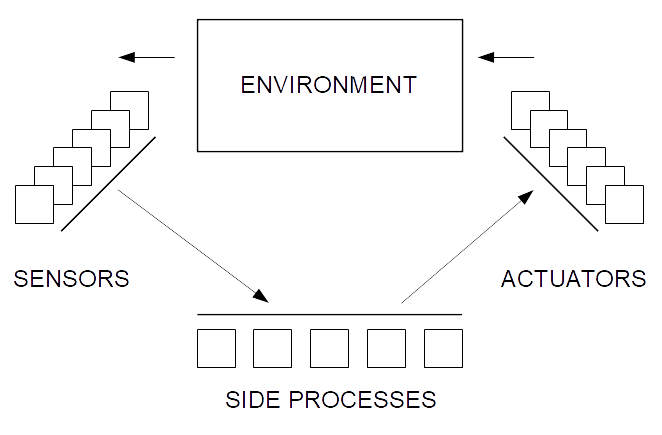
\includegraphics[scale=0.5]{{FIGURES/reacts.png}}\\
\caption{A reactive system.}%
\end{center}
\end{figure}%

One immediate application area for \smurph\ is
any industrial system that can be represented by a network of sensors and
actuators.
The primary goal of {\smurph}
is to provide a platform for developing, testing, and executing
control programs for ``intelligent'' networks of sensors and actuators that
may be interconnected or accessed via the Internet.

\subsection{Control}
\label{rm_in_rv}

\smurph\ offers an
object-oriented programming language for implementing control programs for
reactive systems.
Programs expressed in this language are executed by the \smurph\ kernel that
interfaces them to networks of sensors and actuators and coordinates their
multiple threads.

Besides conventional tools for program debugging, such as local
assertions and tracing functions, \smurph\ offers means for
verifying compound dynamic conditions that can be viewed as an alternative
specification of the control program.
These tools, the so-called {\em observers},
are thread-like objects that can be used for expressing global
assertions involving the combined behavior of more than one regular thread.
As regular assertions verify some Boolean properties of a program, observers
verify state transitions in a distributed system and make sure that these
transitions conform to a set of specifications.
In this sense, observers are conformance testing tools.

A control program in \smurph\ can be implemented as a single multithreaded,
event-driven module, or as a set of modules run on independent (possibly
diverse) machines connected via the Internet.
These modules can communicate with operators (human supervisors)
on other machines via standard Internet browsers capable of running Java
applets.
One can enhance the reliability of a
control program by providing several copies/versions of a single module.
Those multiple copies can be programmed differently, e.g., by different people,
and they can be run on different machines at different geographical locations,
yet they may end up controlling the same physical fragment of the system.

\subsection{Simulation}
\label{rm_in_si}

One distinct feature of \smurph\ is the possibility of replacing fragments of
the interface to a real reactive system with their simulated counterparts.
This way, it is possible to develop, test, and debug a control program
together with the development, testing, and debugging of the underlying
physical system to be controlled.
No part of the control program need be aware of whether the program is run in
a real or artificial environment.

If we ignore the interface of the {\smurph}
kernel to the physical world (and assume that the environment is fully virtual),
we get a simulation package oriented
towards modeling communication networks at the implementation level.
\smurph\ has many standard features of simulators, e.g.,
random number generators and tools for collecting performance data.
As we explained in \sect{rm_in_hi}, before it became an execution platform,
\smurph\ (or rather its predecessor dubbed {\sc SMURPH})
had been a pure simulation package.
None of its simulation-oriented features have been removed in the present
version; consequently, \smurph\ is 100\% compatible
with {\sc SMURPH} and it can be used directly to run simulation
experiments expressed in {\sc SMURPH} (which come included with this
package).

\subsection{Overview}
\label{rm_in_ov}

\smurph\ is a programming language for describing reactive systems
(e.g., communication networks) and specifying event-driven programs
(e.g., network protocols) in a natural and straightforward way.
Programs in \smurph\ are run on a virtual ``hardware'' configured by the user.

\smurph\ can be viewed both as
an implementation of a certain protocol specification language and an
``executor'' (kernel) for running programs expressed in that language.
This kernel can operate in three modes:

In the {\em real mode}, at least some elements of the program's
environment are real and the program is expected to respond to actual
events indicated by physical sensors, and/or trigger actions of some
real actuators.
In such a case, the time flow is real.
Even if there exist simulated components in the environment, they
must behave as real components with respect to the timing of
events triggered and perceived by them.

In the {\em simulation mode}, there is no single real element in the
environment, and the kernel operates as an event-driven
discrete-time simulator.
Events triggered and perceived by the control program occur in virtual time
that usually has no relation to the execution time as perceived by the user.

In the {\em visualization mode}, the system is entirely virtual
(pure simulation); however, the program tries to match virtual
time intervals to their real time counterparts, as specified by the user.
This way, the on-line behavior of the model {\em visualizes\/} the
behavior of the ``real thing,'' possibly up to a certain factor.
It is possible to interact with a model run in the {\em visualization mode.}
For example, such a model can accept external input (and produce output)
in a way essentially the same as a control program interacting with external
devices.
One fundamental difference between the visualization mode and
the real mode is that there are no restrictions in the former on what kind of
events make sense.
In particular, channel models are illegal (impossible) in the real mode because
a channel model cannot correspond to a sensible
real object directly perceptible by the control program.
On the other hand, modeling channels in the visualization mode is OK because
we do not have to worry about the straightforward
correspondence of all aspects of the model to the world located outside
the simulator.

\smurph\ has been programmed in C++ and its protocol specification language
is an extension of C++.
In this manual, we assume that the reader is familiar with C++
and the general concepts of object-oriented programming.

%%%struct.gif
\begin{figure}[htbp]%
\begin{center}
%\ \psfig{figure=FIGURES/struct.ps}
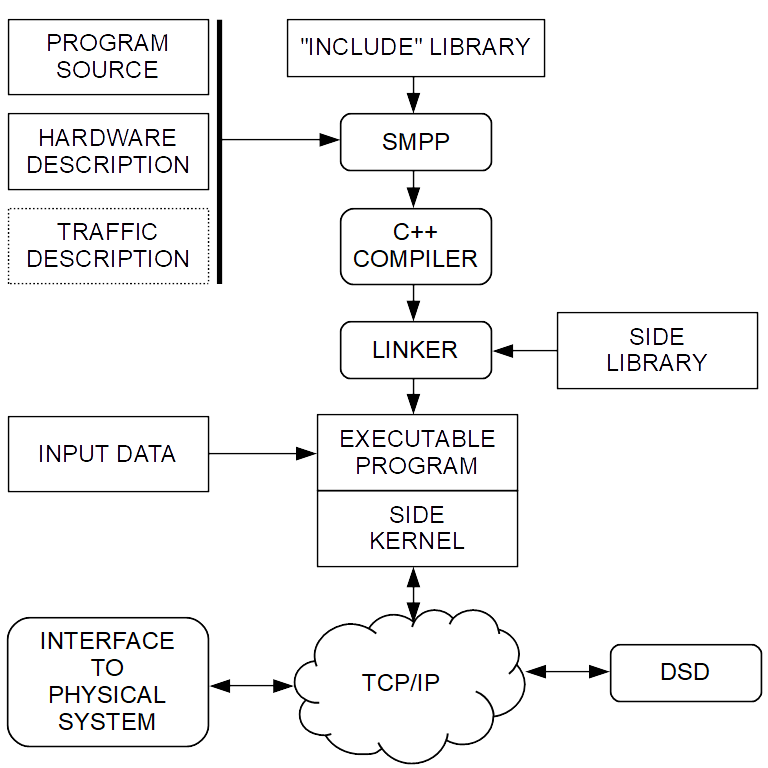
\includegraphics[scale=0.5]{FIGURES/struct.png}
\caption{The structure of \smurph.}%
\end{center}
\end{figure}%

The structure of \smurph\ is presented in
figure 2.
A program in \smurph\ is first preprocessed by {\tt smpp}
to become a C++ program.
The code in C++ is then compiled and linked with the \smurph\ run-time
library.
This operations are organized by
{\tt mks}---a generator script
that accepts as arguments a collection of program files and options, and
creates a stand-alone module,
which is an executable control program or simulator
for the system described by the source file and input data.
If we are interested exclusively in simulation, the resultant program can
be fed with some input data and run ``as is'' to produce performance results.
\smurph\ is equipped with the standard features of simulators, like
random number generators and tools for collecting performance data.

The program in \smurph\ runs under the supervision of the {\smurph}
kernel, which coordinates the multiple
threads ({\em processes\/}) of the program, schedules events, and
communicates the program with the outside world.
The program can be monitored on-line via \dsd\footnote{\dsd\ stands for
{\em Dynamic Status Display.}}---a Java applet that
can be invoked, e.g., from a web browser.
This communication is carried out through a monitor server that typically
runs on a dedicated host visible by both parties (i.e., the program
and \dsd).
\dsd\ is useful for debugging and peeking at the partial
results of a potentially long simulation experiment.

%%%CHKP Simulation experiments in \smurph\ can be checkpointed, swapped out, and
%%%CHKP later restarted, possibly on another machine of the same type.
%%%CHKP There exists a simple tool, dubbed \serdel,\footnote{Supervisor for
%%%CHKP Executing Remote Distributed Experiments on a LAN.
%%%CHKP \serdel\ is described in a separate document that comes with the
%%%CHKP package.}
%%%CHKP which is useful for organizing multiple simulation experiments and distributing
%%%CHKP them among workstations connected into a local network.
%%%CHKP \serdel\ monitors the load of those workstations, starts new experiments
%%%CHKP when workstations become available, swaps out experiments in progress when
%%%CHKP it detects interactive jobs on the workstations, etc.
%%%CHKP Of course, checkpointing makes little sense for control programs driving
%%%CHKP real systems.

Although \smurph\ does not purport to be a protocol verification system,
it offers some tools for protocol testing.
These tools, the so-called {\em observers}, look like programmable
assertions describing sequences of protocol actions.
In fact, they provide an alternative (static) way of specifying the protocol;
it is checked in run-time whether the two specifications agree.

For the purpose of simulation, the source program in \smurph\ is logically
divided into three parts (see~
figure~3).
The protocol part represents the dynamics of the modeled system.
The network part is a logical description of the hardware on which the
protocol program is expected to run.
Finally, the traffic part describes the load of the modeled
system, i.e., the events arriving from the ``virtual outside'' and their
timing.

%%% struct2.gif
\begin{figure}[htbp]%
\begin{center}
%\ \psfig{figure=FIGURES/struct2.ps}
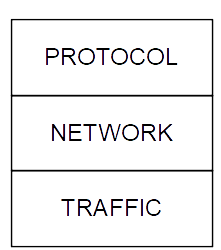
\includegraphics[scale=0.5]{FIGURES/struct2.png}
\caption{Components of a \smurph\ program.}%
\end{center}
\end{figure}%


The terms ``protocol'' and ``traffic'' reflect the fact that the primary
application of {\smurph}'s predecessor was simulating communication
networks.
However, it still makes sense to call a control program driving a network
of sensors and actuators a {\em protocol}, because, owing to its reactive
nature, such a program looks like a set of rules prescribing actions to be
taken upon some specific events that may be coming from several different
(and distant) sources.
Similarly, it makes sense to talk about the input {\em traffic\/} in a
(simulated) fragment of a reactive system, because such a system typically
handles some objects arriving from the outside, and it is natural to
represent such objects as structured {\em packets}.

%%% struct3.gif
\begin{figure}[htbp]%
\begin{center}
%\ \psfig{figure=FIGURES/struct3.ps}
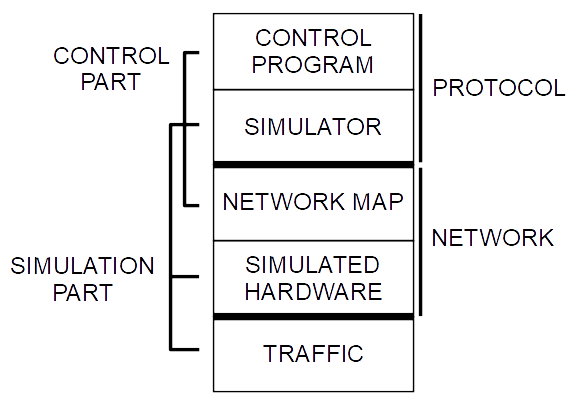
\includegraphics[scale=0.5]{FIGURES/struct3.png}
\caption{A control program in {\smurph}.}%
\end{center}
\end{figure}%

For the purpose of developing control programs in \smurph, we
may adopt a slightly
more elaborate view of the source program (see
figure~4).
The protocol (i.e., the collection of processes) consists now of two parts:
the control program proper and the simulator for the virtual components of
the driven system.
Similarly, the network part is split into the so-called {\em network map},
i.e., the mapping of logical sensors and actuators perceived by the
control program onto their real (or simulated) counterparts,
and the description of the modeled fragments of the underlying hardware, i.e.,
the hardware used by the simulator part of the protocol.
The traffic specification only applies to the simulated part of the environment
(real fragments handle real traffic that need not be specified).

With the above view, one can separate the software components that
belong to the control system from those belonging to the simulator.
Thus, the ``control program'' + ``network map'' comprise the actual
control system (this part represents the target of the development
process, with the network map interpreted as a parameterization of the
control program), while the remaining components will tend to vanish,
until they ultimately disappear altogether in the complete version of
the system.

The system controlled by a \smurph\ program is perceived by that program
as a collection of sensors and actuators represented by
{\em mailboxes\/} (\sect{rm_mb}).
The actual mapping of a sensor/actuator mailbox into its real physical
counterpart consists of two steps.
The lower-level portion of this mapping is carried out by a {\em daemon\/} that
interfaces a physical network of sensors/actuators to the Internet.
The daemon acts as a server
intercepting all status change events in the sensor network and transforming
them into TCP/IP packets sent to the clients.
Similarly, it receives status change requests from its Internet
clients and transforms them into new values of actuators.

On the \smurph\ end, the sensor/actuator resulting from this mapping is
visible as a mailbox bound to a TCP/IP
port.\footnote{A mailbox can also be bound to a device, i.e., a serial
port.
Such a mailbox directly represents the device and makes it visible
to \smurph\ as a reactive object.}
Technically, this perception is sufficient to implement a control program
operating directly on such a mailbox.
However, it usually makes better sense to impose one more level of mapping,
i.e., to transform the raw sensor/actuator mailbox presented by the
daemon into a generic and more uniform object.
The second level of mapping is performed by the network map portion of the
protocol program in {\smurph}, and its advantages are listed below.

\begin{itemize}
\item
The control program can be built in a way independent of the technical
idiosyncrasies of different sensors/actuators manufactured by
different vendors.
\item
It is possible to have a single logical sensor/actuator mapped into several
real sensors/actuators and vice versa.
\item
It is easy to change the mapping of a logical sensor/actuator without affecting
the control program.
For example,
the same logical sensor/actuator may be mapped differently
in different versions of the control program (e.g., it may be simulated
in some versions or mapped to a physical sensor/actuator in others).
\end{itemize}

%%%@@@-- lexic.tex
\section {Lexical notes: naming conventions}
\label{rm_ln}

\smurph\ constitutes a layer of types, objects,
operations and library functions imposed on C++.
Thus, the protocol specification language accepted by the package consists
of C++ augmented by some additional rules and constructs.
We assume that the reader is familiar with C++ and the features of this
language will not be
discussed in this manual, unless they are essential for understanding
some \smurph-specific notions.

The following rules were followed when
introducing \smurph-specific names into the protocol specification language.

The names of global variables and user-visible object attributes
not being methods
start with a capital letter and may contain both lower and upper case
letters.
If the name of a variable has been obtained by putting together a number of
words, then each word starts with a capital letter and all other letters are
in lower case.
Examples of such names are: {\tt Time}, {\tt Itu}, {\tt s->MQHead}.

The names of functions and object methods start with a lower case letter
and may contain both upper and lower case letters.
If the name of a function has been obtained by putting together a number of
words, each word, except the first one, starts with a capital letter and all
other letters are in lower case.
Examples: {\tt setLimit(100)}, {\tt pkt->frameSize()}.

The names of operations
that are intentionally new keywords added to the
language start with lower case letters and contain lower case letters only.
Examples: {\tt station~A~:~B~\{}, {\tt proceed~NewState;}.
The names of macros that are supposed to look as functions or methods
obey the same rules as the names of functions or methods.
Similarly, the names of macros providing aliases for global variables obey
the same rules as the names of variables.
Examples: {\tt idToStation(i)}, {\tt TheStation}, {\tt Timer}.

The name of a symbolic constant (defined as a macro) starts with a sequence of
capital letters optionally followed by a ``{\tt \_}'' (underscore) and a
sequence of lower case letters (and possibly digits).
Examples: {\tt YES}, {\tt MIT\_exp}, {\tt BIG\_precision}, {\tt PF\_usr3}.

There exist some global variables, types, and functions
that are not intended to be visible to the user.
The names of such variables and types begin with ``{\tt zz\_}'' or ``{\tt ZZ\_}''.
Most of the user-invisible methods are made private or protected
within their objects.

%%%@@@-- exten.tex
\section {Extensions of standard arithmetic}
\label {rm_mp}

Having been built on top of C++, \smurph\ naturally inherits all the
arithmetic machinery of that language.
Most of the extensions to this machinery result from the need for a
high precision representation of the modeled discrete time.
This issue is usually less serious in control programs (where the time
resolution of the order of microseconds is typically sufficient) than in
simulators (where the fine granularity of time helps identify race conditions
and other timing problems).

\subsection {Simple integer types}
\label {rm_mp_si}

Different machines may represent types {\tt int}
and {\tt long} using different numbers of bits. 
Moreover, some machines/compilers may offer multiple non-standard
representations for integer numbers.\footnote{E.g., type {\tt long~long}.}
To alleviate the portability problems that may result from different representation
of the integer types on different computers,
\smurph\ defines its private aliases for the most critical of those types.
It is recommended that \smurph\ programs use these aliases instead of the
standard types, at least in the cases when a non-trivial minimum precision must be
guaranteed for a particular object.
Specifically, the package defines the following types:
\medskip

\begin{quote}
\noindent\hspace{-0.35in}{\bf {\tt Long}}\\ \hspace{0in}
This type is intended to represent numbers with a sufficient precision to
cover the range of object {\tt Id}s (see \sect{rm_st_on}).
Generally, type {\tt Long} should be used for integer numbers (possibly signed)
which require more than 16 but no more than 32 bits of precision.
(\smurph\ assumes that numbers belonging to the standard type {\tt int} are
represented on at least 16 bits.)
The guaranteed precision of type {\tt Long} is 24
bits.\footnote{Typically, type
{\tt Long} is defined as {\tt long} and its actual precision is 32 bits.}
\end{quote}

\begin{quote}
\noindent\hspace{-0.35in}{\bf {\tt LONG}}\\ \hspace{0in}
This type represents the maximum-precision signed
integer numbers available on a given machine.
Type {\tt LONG} is used as the base type for creating numbers of type {\tt BIG}
(see \sect{rm_mp_vr}).
\end{quote}

\begin{quote}
\noindent\hspace{-0.35in}{\bf {\tt IPointer}}\\ \hspace{0in}
This is the smallest signed integer type capable of holding a pointer, i.e., an
address.
\end{quote}

\begin{quote}
\noindent\hspace{-0.35in}{\bf {\tt LPointer}}\\ \hspace{0in}
This is the smallest type capable of holding both a pointer and a {\tt LONG} integer
number.
\end{quote}\medskip

The distinction between the above integer types becomes meaningful for 
architectures that offer 64-bit integer arithmetic.
For example, on a 64-bit system, type {\tt int} may be
represented on 32 bits, whereas
both {\tt long} integers and pointers are 64-bit long.
On such a machine, {\tt Long} is equivalenced to {\tt int} and the remaining
three types (i.e., {\tt LONG}, {\tt IPointer}, and {\tt LPointer}) are all
defined as {\tt LONG}.

On a 32-bit system (considered obsolete),
where types {\tt int} and {\tt long}, as well as the pointer
type, are all 32-bit long, types {\tt Long}, {\tt LONG}, and {\tt LPointer}
are set to {\tt long}, and type {\tt IPointer} is declared as {\tt int}.
With the machines/compilers that offer the type {\tt long~long}, the user may select
this type as the base type for creating type {\tt BIG} (see \sect{rm_un_in}).
In such a case, types {\tt LONG} and {\tt LPointer} will be declared as
{\tt long~long}, type {\tt Long} will be equivalenced to {\tt long}, and type
{\tt IPointer} will be defined as {\tt int} (unless the pointer size is wider
than the size of {\tt int}).
Other combinations are conceivable, depending on the subtleties of the machine
architecture and the assortment of integer types offered by the compiler.

\subsection {Time in \smurph}
\label {rm_mp_ti}

As all simulators, \smurph\ provides tools for
modeling the flow of time in a class of physical systems.
Time in \smurph\ is discrete, which means that integer numbers are used
to represent time instants and intervals.

In \smurph, the user is responsible for choosing the granularity of the
modeled time (which can be practically arbitrarily fine).
This granularity is determined by the physical interpretation
of the time unit---the interval between two consecutive time instants.
This interval is called the {\em indivisible time unit\/} and is denoted
by {\em ITU}.
In the virtual (simulation) mode,
the correspondence between the {\em ITU\/} and an interval of real time
is not defined explicitly.
All time-dependent quantities are assumed to be relative to the {\em ITU},
and it is up to the interpreter of the input data and output results
to assign a meaning to it.
In the real mode, by default, one {\em ITU\/} is equal to one microsecond
of real time.
This binding can be redefined by the user.
In the visualization mode, the user must set up the correspondence between
the internal time unit and an interval of real time.
This correspondence must be explicitly established when the visualization
mode is entered (\sect{rm_pr_vi}).

If two events modeled by \smurph\ occur within the same {\em ITU}, there
is generally
no way to order them with respect to their ``actual'' succession in time.
In many cases (especially in any of the two simulation modes)
the order in which such events are presented (trigger some
operations in the user program) is nondeterministic.
It is possible, however, to assign priorities to awaited events.
This way, when multiple events occur at the same time, they will be
presented in the order of their priorities.
It is also possible (see~\sect{rm_un_cr}) to switch off the nondeterminism
in \smurph\ (which is generally much less desirable in control than in
simulation).
Of course, events triggered by actual physical components of a controlled
system always occur at some specific real-time moments.

Besides the {\em ITU}, there exist two other time-related units, whose role
is to hide the internal time unit and simplify the interpretation of input
and output data.
One of them is {\em ETU}, i.e., the
{\em experimenter time unit}, which determines the primary unit of time being of
relevance to the user.
The user declares the correspondence between the {\em ITU\/} and the {\em ETU\/}
by calling one of the following two functions:
\begin{verbatim}
        void setEtu (double e);
        void setItu (double i);
\end{verbatim}
The argument of {\tt setEtu}
specifies how many {\em ITU\/}s are in one {\em ETU};
the argument of {\tt setItu}
indicates the number of {\em ETU\/}s in one {\em ITU};
The call
\begin{verbatim}
        setEtu (a);
\end{verbatim}
is equivalent to the call:
\begin{verbatim}
        setItu (1/a);
\end{verbatim}
One of the two functions
should be called only once, at the beginning of the network
creation phase, before the first object of the network is created
(\sect{rm_to}).
Two global, read-only variables {\tt Itu} and {\tt Etu} of type {\tt double}
tell the relationship between the {\em ITU\/} and {\em ETU}.
{\tt Itu} contains the number of {\em ETU\/}s in one {\em ITU\/} and
{\tt Etu}, the reciprocal of {\tt Itu}, contains the number of {\em ITU\/}s
in one {\em ETU}.

The current simulated time in {\em ITU\/}s is available via two global (intentionally read-only) variables declared as:
\begin{verbatim}
        TIME Time;
        double ETime;
\end{verbatim}
\noindent
The type {\tt TIME} is introduced in \sect{rm_mp_vr}.
The first variable tells the simulated time in {\em ITU\/}s while the seconds one does it in {\em ETU\/}s.\footnote{This variable is in fact a macro.}

The third unit is called {\em DU}, which stands for {\em distance unit}.
Its purpose is to establish a convenient measure of distance (typically
propagation distance between network nodes), which internally translates into
a specific number of {\em ITU\/}s required by the signal to travel the given
distance.
The function:
\begin{verbatim}
        void setDu (double i);
\end{verbatim}
sets the {\em DU\/} to the specified number of {\em ITU\/}s.
The corresponding global variable (of type {\tt double} is called {\tt Du},
and it contains the number of {\em ITU\/}s in one unit of propagation
distance.

For illustration,
suppose that you want to model a mobile wireless network operating
at 100Mb/s, with the mobility grain of $10$cm.
Assuming the signal propagation speed of $3 \times 10^8$m/s, the amount of
time corresponding to $10$cm is $1/(3 \times 10^9 ) = 0.33 \times 10^{-9}$s.
You want the {\em ITU\/} to be at least as small as this number.
Also, you have to keep in mind that the transmission rate of
a transceiver (or port) should be expressible as an entire number of
{\em ITU\/}s per
bit (see sections \ref{rm_to_tr_cr}, \ref{rm_to_po_cr}).
At 100Mb/s, one bit translates into $10^{-8}$s; thus, it may make sense to
assume that 1~{\em ITU\/} corresponds to $0.33 \times 10^{-9}$s.
By issuing the following two calls:
\begin{verbatim}
        setEtu (3000000000.0);
        setDu (10.0);
\end{verbatim}
you set the {\em ETU\/} to $1$s and the {\em DU\/} to $1$m.
Also, the transmission rate of transceivers (\sect{rm_to_tr_cr})
should then be set to $30$, which is the number of {\em ITU\/}s needed to insert
a single bit into the wireless channel.
Note that the {\em ITU\/} is never defined explicitly: its meaning is
determined by the values of the remaining two units, as well as by the
transmission rate assigned to ports and/or transceivers.

In the real mode, the {\em DU\/} is not used
(the concept of propagation distance only applies
to the models of communication channels), and
the {\em ETU\/} stands for one real second.
There exists an alias for {\tt Etu}, namely {\tt Second};
instead of {\tt setEtu}, you can use {\tt setSecond} with the same
result.
These functions give you a means to define the internal granularity of time.
By default, {\tt Second} ({\tt Etu}) is set to 1,000,000 (and {\tt Itu}
contains 0.000001), which means that one {\em ITU\/} is equal to one
microsecond.

The visualization mode brings no restrictions compared to the
virtual mode; however, it makes sense to agree to interpret the
{\em ETU\/} as one second.
This is because the operation of entering the visualization mode
(\sect{rm_pr_vi}) specifies the number of real 
milliseconds to be used as the synchronization grain (at those intervals
the simulator will be synchronizing its virtual time to real time)
and associates with it a given fraction of {\em ETU}.
For clarity, {\em ETU\/} should correspond to some well-known interval, and
one second seems to be a safe bet.

To continue the above example, suppose that you would like to visualize
the behavior of your network with the granularity of $1/4$s, assuming that
one virtual second spreads over ten seconds of real time.
This is the operation to enter the visualization mode:
\begin{verbatim}
        setResync (250, 0.025);
\end{verbatim}
\noindent
The first argument gives 250 millisecond as the ``resync granularity,''
and the second one maps these 250 milliseconds (of real time) to
0.025~{\em ETU\/}s.
Thus, assuming that 1 {\em ETU\/} stands for
1 second of virtual time, one second of
real time will correspond to 1/10 of a second in the model.
This means that the
visualization will be carried out in slow motion with the
factor of 10.

\medskip

\noindent
{\bf Note:} The functions introduced above are not available when
the simulator (or rather the control program) has been compiled with
{\tt -F} (\sect{rm_un_cr}).
In such a case, the {\em ETU\/} is ``hardwired'' at 1,000,000
{\em ITU\/}s ({\tt Etu}, {\tt Itu}, and {\tt Second} are not available
to the program).

\medskip

In both simulation modes,
{\tt Itu}, {\tt Etu}, and {\tt Du} all start equal to 1.0,
and there is no implicit interpretation of the internal time unit with
respect to real time.
It is illegal to redefine the {\em ETU\/} after the visualization mode
has been entered.
Note, however, that the visualization mode can be exited and entered
dynamically (\sect{rm_pr_vi}).

If the same program is supposed to run in a simulation mode as well as in
the control mode, it usually makes sense to put the statement:
\begin{verbatim}
        setEtu (1000000.0);
\end{verbatim}
\noindent
somewhere in the initialization sequence (\sect{rm_pr_or}).

While operating in the real or visualization mode,
a \smurph\ program maps intervals of
virtual time to the corresponding intervals of real time.
The actual knowledge of real time (the precise date and time of the day) is
usually less relevant.
One place where actual time stamps are used is journaling
(\sect{rm_mb_ju}), which is available in the real as well as the
visualization mode.
Such time stamps are represented as the so-called UNIX time, i.e.,
the number of seconds and microseconds that have elapsed
since 00:00:00 on January 1, 1970.
The following function:
\begin{verbatim}
        Long getEffectiveTimeOfDay (Long *usec = NULL);
\end{verbatim}
returns the number of seconds in UNIX time.
The optional argument is a pointer to a {\tt Long} number which,
if specified, will contain the number of microseconds after the
last second.
Function {\tt tDate} (\sect{rm_au_td})
converts the value returned by {\tt getEffectiveTimeOfDay} into a textual
representation of the current date and time.

It is possible to call a \smurph\ program operating in the real or
visualization mode in such a
way that its real time is shifted to the past or to the future.
This may be useful together with journaling (\sect{rm_mb_ju}), e.g.,
to synchronize the program to a past journal file.
The {\tt -D} call argument (\sect{rm_un_ru}) can be used for this purpose.
If the real time has been shifted, both {\tt getEffectiveTimeOfDay} and
{\tt tDate} return the shifted time.

\subsection {Type {\tt BIG} and its range}
\label {rm_mp_vr}

In many cases the standard range of integer numbers available on the given
machine is insufficient to represent long intervals of simulated time with a
satisfying granularity.
Therefore, \smurph\ comes with its own type for representing potentially
huge {\bf nonnegative} integer numbers and performing standard arithmetic
operations on them.

Time instants and other potentially huge nonnegative integers should be
declared as objects of type {\tt BIG} or {\tt TIME}.
These two types are absolutely equivalent.
Intentionally, {\tt TIME} should be used in declarations of variables
representing time instants or
intervals and {\tt BIG} can be used to declare other big integers, not
necessarily related to time.

When a \smurph\ program is created by {\tt mks} (see \sect{rm_un_cr}),
the user may specify the precision of type {\tt BIG} with the {\tt -b}
option.
The value of this option (a single decimal digit) is passed
to \smurph\ (and also to the user program) in
symbolic constant {\tt BIG\_precision}.
This value selects the implementation of type {\tt BIG} by specifying the
minimum guaranteed precision of {\tt BIG} numbers as
{\tt BIG\_precision}$\times 31$ bits.
If {\tt BIG\_precision} is 1 or 0,
type {\tt BIG} is equivalent to the maximum-length integer type available on
the given machine (type {\tt LONG}---see \sect{rm_mp_si})
and all operations on objects of
this type are performed directly as operations on integers of type {\tt LONG}.
Otherwise,
depending on the size of type {\tt LONG}, several objects of this type
may be put together to form a single {\tt BIG} number.
For example, if the size of {\tt LONG} is 32 bits,
a single {\tt BIG} number is represented as {\tt BIG\_precision}
{\tt LONG} numbers.
If the {\tt LONG} size is 64 bits,
the number of {\tt LONG}
objects needed to form a single {\tt BIG} number is equal to\footnote{Thus,
for {\tt BIG\_precision} equal 1 and 2, {\tt BIG} numbers
will be represented in the same way, using the standard integer type {\tt long}.}
\[
\lfloor \frac{{\tt BIG\_precision}+1}{2} \rfloor~~.
\]

The tacit limit on the precision of type {\tt BIG} imposed by {\tt mks}
(\sect{rm_un_cr}) is 9 which corresponds to 279 significant bits.
Using this precision one could simulate the life of the universe with the
granularity of time corresponding to the Planck interval.

The default precision of type {\tt BIG} is 2 (in both modes).
For the real mode, assuming that one {\em ITU\/}
is equal to one microsecond, the amount of real time covered
by the range of type {\tt BIG} (and {\tt TIME}) is almost 150,000 years
(but it is only slightly more that 30 minutes for precision 1).

\subsection {Arithmetic operations and conversions}
\label {rm_mp_ao}

The actual implementation of type {\tt BIG} is completely transparent to
the user.
When the precision of {\tt BIG} numbers is different from 1, the standard
arithmetic operators {\tt +}, {\tt -}, {\tt *}, {\tt /}, {\tt \%}, {\tt ++},
{\tt --}, {\tt ==}, {\tt !=}, {\tt <}, {\tt >}, {\tt <=}, {\tt >=}, {\tt +=},
{\tt -=}, {\tt *=}, {\tt /=}, {\tt \%=} are automatically overloaded to operate
on objects of type {\tt BIG}.
Combinations of {\tt BIG} operands with types {\tt int}, {\tt long},
and {\tt double} are legal.
If {\tt BIG} is equivalent to {\tt long}, the conversion rules for operations
involving mixed operand types are defined by C++.
Otherwise, if an operation involves a {\tt BIG} operand mixed with
a numerical operand of another type, the following rules are used:
\begin{itemize}
\item
If the type of the other operand is {\tt char}, {\tt int}, or {\tt long},
the operand is converted to {\tt BIG} and the result type is {\tt BIG}.
One exception is the modulo ({\tt \%}) operator with the second operand
being of one of the above types.
In such a case, the second operand is converted to {\tt long} and the result
type is {\tt long}.
\item
If the type of the other operand is {\tt float} or {\tt double}, the {\tt BIG}
operand is converted to {\tt double} and the result type is {\tt double}.
\item
An assignment to/from {\tt BIG} from/to other numerical type is legal and
involves the proper conversion.
A {\tt float} or {\tt double} number assigned to {\tt BIG} is truncated to
its integer part.
\end{itemize}

Overflow and error conditions for operations involving
{\tt BIG} operands are only checked for precisions 2--9.\footnote{If the size
of type {\tt LONG} is 64 bits, the overflow and error conditions are only
checked for precisions higher than 2.}
You can switch off those checks (e.g., for efficiency) with
the {\tt -m} option of {\tt mks} (see \sect{rm_un_cr}).
Note that in principle it is illegal to assign a negative value to a
{\tt BIG} variable.
However, for precisions 0 and 1 such operation passes unnoticed and
the problem will surface later.

It is possible to check whether a {\tt BIG} number is convertible to
{\tt double}.
The following function:
\begin{verbatim}
        int convertible (BIG a);
\end{verbatim}
returns 1, if the {\tt BIG} number {\tt a} can be safely
converted to {\tt double}, and 0 otherwise.

Explicit operations exist for converting a character string (an unsigned
sequence of decimal digits) into a {\tt BIG} number and vice versa.
The following function turns a {\tt BIG} number into a
sequence of characters:
\begin{verbatim}
        char *btoa (BIG a, char *s = NULL, int nc = 15);
\end{verbatim}
where {\tt a} is the number to be converted to characters, {\tt s} points
to an optional character buffer to contain the result, and {\tt nc}
specifies the length of the resulting string.
If {\tt s} is not specified (or {\tt NULL}) an internal (static)
buffer is used.
In any case, the pointer to the encoded string is returned as the function
value.

If the number size exceeds the specified string capacity (15 is the default),
the number is encoded in the format: {\tt dd...ddEdd}, where {\tt d} stands
for a decimal digit and the part starting with {\tt E} is a decimal exponent.

The following function can be used to convert a string of characters into
a {\tt BIG} number:
\begin{verbatim}
        BIG atob (const char *s);
\end{verbatim}

The character string pointed to by {\tt s} is processed until the first
character that is not a decimal digit is encountered.
Initial spaces and an optional plus sign are ignored.

\subsection {Constants}
\label {rm_mp_co}

One way to create a constant of type {\tt BIG} is to convert a
character string into a {\tt BIG} object.
If the constant is not too big,
one can use a conversion from {\tt long~int}, e.g.,
{\tt b~=~22987} (we assume that {\tt b} is of type {\tt BIG})
or {\tt double}.
This works also in declarations; thus, the following examples are legal:
\begin{verbatim}
        BIG  b = 12;
        TIME tc = 10e9;
        const TIME cnst = 20000000000.5;
\end{verbatim}
are legal.
In the last case, the fractional part is ignored.

Three {\tt BIG} constants:
{\tt BIG\_0}, {\tt BIG\_1}, and {\tt BIG\_inf} are available directly.
The first two of them represent 0 and 1 of type {\tt BIG}, the last
constant stands for an {\em infinite\/} or {\em undefined\/} value and is
equal to the maximum {\tt BIG} number representable with the given
precision.
This maximum value is reserved to denote {\em infinity\/} (or an
{\em undefined\/} value) and it should not
be used as a regular {\tt BIG} number.
For completeness, there exist constants {\tt TIME\_0}, {\tt TIME\_1}, and
{\tt TIME\_inf} which are exactly equivalent to the three {\tt BIG}
constants.

These two predicates tell whether a {\tt BIG} number is {\em defined\/}
(or {\em finite\/}):
\begin{verbatim}
        int def (BIG a);
\end{verbatim}
returning 1 when {\tt a} is defined (or finite) and 0 otherwise, and
\begin{verbatim}
        int undef (BIG a);
\end{verbatim}
which is a simple negation of {\tt def}.

The following arithmetic-related symbolic constants are available to the
protocol program:

\medskip

\begin{quote}
\noindent\hspace{-0.35in}{\bf {\tt TYPE\_long}}\\ \hspace{0in}
equal to 0.
This is a type indicator (see \sect{rm_mp_ot}).
\end{quote}

\begin{quote}
\noindent\hspace{-0.35in}{\bf {\tt TYPE\_short}}\\ \hspace{0in}
equal to 1.
An unused type indicator existing for completeness.
\end{quote}

\begin{quote}
\noindent\hspace{-0.35in}{\bf {\tt TYPE\_BIG}}\\ \hspace{0in}
equal to 2.
This is the {\tt BIG} type indicator (see \sect{rm_mp_ot}).
\end{quote}

\begin{quote}
\noindent\hspace{-0.35in}{\bf {\tt BIG\_precision}}\\ \hspace{0in}
telling the the precision of {\tt BIG} numbers (\sect{rm_mp_vr}).
\end{quote}

\begin{quote}
\noindent\hspace{-0.35in}{\bf {\tt MAX\_long}}\\ \hspace{0in}
equal to the maximum positive number representable with type {\tt long~int}.
For 32-bit 2's complement arithmetic this number is $2147483647$.
\end{quote}

\begin{quote}
\noindent\hspace{-0.35in}{\bf {\tt MIN\_long}}\\ \hspace{0in}
equal to the minimum negative number representable with type {\tt long~int}.
For 32-bit 2's complement arithmetic this number is $-2147483648$.
\end{quote}

\begin{quote}
\noindent\hspace{-0.35in}{\bf {\tt MAX\_short}}\\ \hspace{0in}
equal to the maximum positive number representable with type {\tt short~int}.
For 16-bit 2's complement arithmetic this number is 32767.
\end{quote}

\begin{quote}
\noindent\hspace{-0.35in}{\bf {\tt MIN\_short}}\\ \hspace{0in}
equal to the minimum negative number representable with type {\tt short~int}.
For 16-bit 2's complement arithmetic this number is $-32768$.
\end{quote}

\begin{quote}
\noindent\hspace{-0.35in}{\bf {\tt MAX\_int}}\\ \hspace{0in}
equal to the maximum positive number representable with type {\tt int}.
In most cases this number is equal to {\tt MAX\_long} or {\tt MAX\_short}.
\end{quote}

\begin{quote}
\noindent\hspace{-0.35in}{\bf {\tt MIN\_int}}\\ \hspace{0in}
equal to the minimum negative number representable with type {\tt int}.
In most cases this number is equal to {\tt MIN\_long} or {\tt MIN\_short}.
\end{quote}\medskip

There also exist the following constants: {\tt MAX\_Long}, {\tt MIN\_Long},
{\tt MAX\_LONG}, and {\tt MIN\_LONG} which represent the boundary values of
types {\tt Long} and {\tt LONG}, according to the way these types have been
aliased to the corresponding basic integer types (see \sect{rm_mp_si}).

\subsection {Other non-standard numerical types}
\label {rm_mp_ot}

Some numbers, not necessarily representing time instants or intervals,
may also be potentially big.
On the other hand, using type {\tt BIG} to represent all numbers that
could potentially exceed the capacity of standard types {\tt int} or
{\tt long} would be too costly in typical situations.
Therefore, there exist three flexible
non-standard numerical types that can be used
to represent nonnegative integer variables.
By default, all three types are equivalenced ({\tt typedef}) to type {\tt LONG},
but those defaults can be changed with compilation options
to {\tt BIG} or {\tt Long} (see \sect{rm_un_cr}), depending on whether they are
too tight or still too wasteful.
The three types are:

\medskip

\begin{quote}
\noindent\hspace{-0.35in}{\bf {\tt DISTANCE}}\\ \hspace{0in}
This type is used to represent (internally)
propagation distances between {\em ports\/} or {\em transceivers\/}
(see sections \ref{rm_to_li_pr}, \ref{rm_to_po_co}, \ref{rm_to_tr_if}).
A propagation distance is in fact a time interval; however, in most cases
this interval is reasonably small.
\end{quote}

\begin{quote}
\noindent\hspace{-0.35in}{\bf {\tt BITCOUNT}}\\ \hspace{0in}
This type is used to declare variables counting individual information
bits, e.g., transmitted or received globally or at a specific station.
Numerous such counters are used internally by \smurph\ for calculating
various performance measures.
\end{quote}

\begin{quote}
\noindent\hspace{-0.35in}{\bf {\tt RATE}}\\ \hspace{0in}
This type is used to represent port {\em transmission rates\/}
(see \sect{rm_to_po_cr}).
The transmission rate of a port is a time interval which in most cases
is rather small.
\end{quote}\medskip

Five macros are associated with each of the above three types.
For example, the following macros are related to type {\tt DISTANCE}:

\medskip

\begin{quote}
\noindent\hspace{-0.35in}{\bf {\tt TYPE\_DISTANCE}}\\ \hspace{0in}
This is a symbolic constant which
can have one of two values: {\tt TYPE\_long}~(0) meaning that type
{\tt DISTANCE} is equivalent to {\tt LONG} or {\tt Long},
or {\tt TYPE\_BIG}~(2) which
means that {\tt DISTANCE} is equivalent to {\tt BIG}.
\end{quote}

\begin{quote}
\noindent\hspace{-0.35in}{\bf {\tt MAX\_DISTANCE}}\\ \hspace{0in}
This macro is defined as {\tt BIG\_inf}, {\tt MAX\_LONG}, or
{\tt MAX\_Long}, depending on whether 
type {\tt DISTANCE} is equivalent to {\tt BIG}, {\tt LONG}, or {\tt Long}.
\end{quote}

\begin{quote}
\noindent\hspace{-0.35in}{\bf {\tt DISTANCE\_inf}}\\ \hspace{0in}
The same as {\tt MAX\_DISTANCE}.
\end{quote}

\begin{quote}
\noindent\hspace{-0.35in}{\bf {\tt DISTANCE\_0}}\\ \hspace{0in}
This macro is defined as {\tt 0} if type {\tt DISTANCE} is equivalent to
{\tt LONG} or {\tt Long}, or as {\tt BIG\_0}, otherwise.
\end{quote}

\begin{quote}
\noindent\hspace{-0.35in}{\bf {\tt DISTANCE\_1}}\\ \hspace{0in}
This macro is defined as {\tt 1} if type {\tt DISTANCE} is equivalent to
{\tt LONG} or {\tt Long}, or as {\tt BIG\_1}, otherwise.
\end{quote}\medskip

To obtain the corresponding macros for the other two types, replace
the word {\tt DISTANCE} with {\tt BITCOUNT} or {\tt RATE}.

You should use your judgment, based on the interpretation of {\em ITU\/} and the
expected range of values accumulated in bit counters (like the total length
of all messages received by a node in the course of a simulation run) to 
decide whether the default definitions are fine.
For example, if the {\em ITU\/} corresponds to $1$fs (femto-second, i.e.,
$10^{-15}$s), the
maximum propagation distance covered by a 32-bit {\tt LONG} integer is
slightly over $600$m (assuming $c = 3 \times 10^8$m/s).
Thus, if longer distances are not unlikely to show up in your model (and
{\tt LONG} happens to be 32-bit long), {\tt DISTANCE} should be declared
as {\tt BIG}.
Type {\tt RATE} is generally less prone to this type of problems.
As a rate determines the number of {\em ITU\/}s needed to transmit a single
bit, the lower the actual transmission rate, the higher the value that must
be stored in a {\tt RATE} object.
For illustration,
with 1~{\em ITU\/} corresponding to $1$fs, the maximum interval stored
in a 32-bit number is ca.\ $2^{-6}$s, which translates into the minimum
rate of $500$kb/s.

\medskip

\noindent
{\bf Note:} Rates, bit counts, and distances are only useful when {\smurph}
is used as a network simulator (possibly in the visualization mode).
They are irrelevant in the real mode.

\medskip

The way distances are specified (and usually interpreted)
by the user (e.g., when configuring a network,
see~\sect{rm_to_po_se}) involves {\tt double} numbers, which are internally
transformed into type {\tt DISTANCE} according to the setting of the
{\em distance unit\/} {\em DU\/} (\sect{rm_mp_ti}).
\smurph\ defines the following {\tt double} constants:
{\tt Distance\_0},
{\tt Distance\_1},
{\tt Distance\_inf},
which translate into/from the respective {\tt DISTANCE} values in the
conversion from/to {\tt double} involving the assumed distance unit.
Similarly, as the internal time in {\em ITU\/}s is often converted to 
double precision time in {\em ETU\/}s, the following {\tt double} constants:
{\tt Time\_0},
{\tt Time\_1},
{\tt Time\_inf}
represent {\em ETU\/} equivalents of the respective {\tt TIME} constants.
Even though the conversion between {\em ITU}, {\em ETU\/} and {\em DU\/} is
straightforward (and involves multiplication/division by {\tt Itu}, {\tt Etu}
or {\tt Du}), \smurph\ provides the following functions whose consistent
usage may help to avoid confusion or ambiguity:
\begin{verbatim}
        double ituToEtu (TIME);
        TIME etuToItu (double);
        double itoToDu (TIME);
        TIME duToItu (double);
\end{verbatim}
\noindent
In addition to performing the required scaling, these functions also correctly
convert the special value {\em inf}, e.g.,
{\tt ituToEtu (TIME\_inf) == Time\_inf}.

%%%@@@-- auxil.tex
\section{Auxiliary operations and functions}
\label{rm_au}

In this section we list those functions provided by \smurph\ that are
only superficially related
to its operation as a network simulator or a system controller.
They cover random number generation, non-standard i/o, and a few other
items that are not extremely important, as the user cold easily substitute
for them some standard tools from the C++ library.

In those early days
when the first (C++) version of \smurph\ ({\sc SMURPH}) was being developed,
there was little consensus regarding the exact shape of the C++ i/o library
and other common functions, which tended to differ
quite drastically across platforms.
Consequently, we wanted to cover them as much as possible by our own tools,
such that the same \smurph\ program could compile and run
without modifications on all popular platforms.
These tools are still present in the most recent version of our package,
even though these days the standard libraries are much more consistent than they were when our project started.

\subsection{Random number generators}
\label{rm_au_rn}

All random number generators offered by \smurph\ are based on the following
function:
\begin{verbatim}
        double rnd (int seed);
\end{verbatim}
which returns a pseudo-random number of type {\tt double} uniformly
distributed in [0,1).
By default, this function uses its private
congruential algorithm for generating random numbers.
The user can select the standard random number generator (the {\tt drand48}
family) by creating the program with the
``{\tt -8}'' option (see \sect{rm_un_cr}).

The argument of {\tt rnd} which must be {\tt SEED\_traffic} (0), 
{\tt SEED\_delay} (1), or {\tt SEED\_toss} (2), identifies one of
three {\em seeds}.
Each seed represents a separate pattern of pseudo-random numbers.
The initial values of the seeds (which are of type {\tt long}) can be specified
when the \smurph\ program is called (see \sect{rm_un_ru}); otherwise,
some default (always the same) values are assumed.
This way simulation runs are replicable, which is important from the
viewpoint of debugging.

Intentionally, each of the three seeds represents one category of objects
to be randomized, in the following way:

\medskip

\begin{quote}
\noindent\hspace{-0.35in}{\bf {\tt SEED\_traffic}}\\ \hspace{0in}
Traffic related randomized values (see \sect{rm_cl}), e.g.,
message interarrival intervals, message lengths,
selection of the transmitter and the receiver.
\end{quote}

\begin{quote}
\noindent\hspace{-0.35in}{\bf {\tt SEED\_delay}}\\ \hspace{0in}
Values representing lengths of various (possibly randomized)
delays not related to traffic generation.
For example, randomization of {\tt Timer} delays for modeling
inaccurate clocks (\sect{rm_ti_to}) is based on this seed.
\end{quote}

\begin{quote}
\noindent\hspace{-0.35in}{\bf {\tt SEED\_toss}}\\ \hspace{0in}
Tossing (multi-sided) coins in situations when \smurph\ must
decide which of a number of equally probable possibilities to
follow, e.g., selecting one of two or more waking events scheduled at the
same {\em ITU\/} (see \sect{rm_pr_po}).
\end{quote}\medskip

All random numbers needed by \smurph\ internally are generated according
to the above rules, but the user is not obliged to obey them.
In most cases, the user need not use {\tt rnd} directly.

When the program is restarted with the same value of a given seed, all
randomized objects belonging to the category represented by this seed will be
generated in exactly the same way as previously.
In particular, two
simulation runs with identical values of all three seeds will produce
exactly the same results, unless the declared CPU time limit is exceeded
(\sect{rm_ts_cp}).

The following functions can be used to generate exponentially distributed
pseudo-random numbers:
\begin{verbatim}
        TIME tRndPoisson (double mean);
        LONG lRndPoisson (double mean);
        double dRndPoisson (double mean);
\end{verbatim}

When the precision of {\tt TIME} is 1, the first two functions are identical.
The first function should be used for generating objects
of type {\tt TIME},
while the second one generates ({\tt LONG}) integer values.
The parameter specifies the mean value of the distribution whose type is
{\tt double} in all cases.
The result is generated from a uniformly distributed pseudo-random
value obtained by a call to {\tt rnd} with seed 0 ({\tt SEED\_traffic}).
In the first two cases,
the double precision floating point intermediate result is rounded
to an object of type {\tt TIME} or {\tt LONG}.

Below we present five functions that generate uniformly distributed random
numbers of type {\tt TIME} and {\tt LONG}.
\begin{verbatim}
        TIME tRndUniform (TIME min, TIME max);
        TIME tRndUniform (double min, double max);
        LONG lRndUniform (LONG min, LONG max);
        LONG lRndUniform (double min, double max);
        double dRndUniform (double min, double max);
\end{verbatim}

In all cases the result is
between {\tt min} and and {\tt max}, inclusively.
The functions call {\tt rnd} with seed 0 ({\tt SEED\_traffic}).

Sometimes one would like to randomize a certain, apparently constant,
parameter, so that its actual value is taken with some {\em tolerance}.
The following functions serve this end:
\begin{verbatim}
        TIME tRndTolerance (TIME min, TIME max, int q)
        TIME tRndTolerance (double min, double max, int q)
        LONG lRndTolerance (LONG min, LONG max, int q)
        LONG lRndTolerance (double min, double max, int q)
        double dRndTolerance (double min, double max, int q)
\end{verbatim}

The above functions generate random numbers according to the {\em Beta\/}
distribution which is believed to describe technical parameters that may
vary within some tolerance.
The functions call {\tt rnd} with seed 1
({\tt SEED\_delay}) and transform the uniform distribution into distribution
\[
\beta (q, q)
\]
\noindent
which is scaled appropriately, such that the resultant random
number is between {\tt min} and {\tt max} inclusively.
The parameter {\tt q}, which must be greater than 0,
can be viewed as the ``quality'' of the distribution.
For higher values of
{\tt q} the generated numbers have better chances to be closer to
({\tt min}+{\tt max})/2.
Reasonable values of {\tt q} are between 1 and 10.
Slightly more time is taken for generating a random number for a higher
value of {\tt q}.

The following function generates a normally distributed (Gaussian) random
number:
\begin{verbatim}
        double dRndGauss (double mean, double sigma);
\end{verbatim}
with the specified mean and standard deviation.
It calls {\tt rnd} with seed 2 ({\tt SEED\_toss}).

Here is a function to generate a randomized number of successes in a
Bernoulli experiment involving tossing a possibly biased coin:
\begin{verbatim}
        Long lRndBinomial (double p, Long n);
\end{verbatim}
\noindent
where {\tt p} is the probability of success in a single experiment, and {\tt n}
is the total number of trials.

Various instances of practical Zipf-style distributions can be produced with
this function:
\begin{verbatim}
        Long lRndZipf (double q, Long max = MAX_Long, Long v = 1);
\end{verbatim}
which generates integer random values between 0 and {\tt max}--1, inclusively,
in such a way that the probability of value $k$ being selected is proportional
to:
\[
P_k = \frac{1}{(v + k)^q}\;\;\;\;(k = 0, \ldots, \texttt{max}-1)
\]
Note that {\tt v} must be greater than zero, and {\tt q} must be greater
than 1.

The following function simulates tossing a multi-sided coin:
\begin{verbatim}
        Long toss (Long n);
\end{verbatim}
It generates an integer number between 0 and {\tt n}--1
inclusively. Each number from this range occurs
with probability 1/{\tt n}. The function calls {\tt rnd} with seed 2
({\tt SEED\_toss}).

There is an abbreviation for the most frequently used variant of {\tt toss},
namely, the following function:
\begin{verbatim}
        int flip ();
\end{verbatim}
returns 0 or 1, each value with probability 0.5.
This function is slightly more efficient than {\tt toss~(1)}.

\subsection{Input/Output}
\label{rm_au_io}

Two standard files, dubbed the {\em data\/} file and the {\em results\/}
file, are automatically opened by a \smurph\ program at the beginning of
its execution.
For a simulation experiment, the results file is supposed to contain the
final performance results at the end of run.
In a control session, the results file may not be needed, although it
may still make sense to produce some ``permanent'' output, e.g., a log or
some measurement data.

The {\em data\/} file, represented by the global variable {\tt Inf}
of type {\tt istream}, is opened for reading and it may contain some
numerical data parameterizing the system architecture and the protocols, e.g.,
the number of stations, TCP/IP ports of the daemons, the mapping of virtual
sensors/actuators to their physical counterparts, etc.

\medskip

\noindent
{\bf Note:}
The data file is only accessible during the initialization phase,
i.e., while the {\tt Root} process is in its first state (\sect{rm_pr_or}).
The file is closed before the protocol execution is started.
If the program requires a continuous stream of data during its execution,
it should open a non-standard input file with that data, or, perhaps, read
the data from a bound mailbox (if it executes in the
real or visualization mode---\sect{rm_mb_gc}).
The same applies to non-standard output files, which, needless to say, a
program may open as many as it needs.

\subsubsection{Reading and writing simple numerical data}
\label{rm_au_io_nd}

All standard functions and methods of C++ related to input/output are
available from \smurph.
There are, however, some additional functions introduced specifically 
by \smurph, which handle input from the data file and output to the
results file.
The most natural way to write some information to the {\em results\/} file
is to {\em expose\/} some objects (\sect{rm_ex}).
In this section we discuss more elementary i/o
operations offered by \smurph.

The standard C++ operators {\tt <<} and {\tt >>} with a stream object as the
first argument have been overloaded to handle {\tt BIG} numbers.
Thus, it is legal to write
\begin{verbatim}
        sp >> b;
\end{verbatim}
or
\begin{verbatim}
        sp << b;
\end{verbatim}
where {\tt sp} is a stream object (it should be an {\tt istream} in the
first case and an {\tt ostream} in the second) and {\tt b} is a number of type
{\tt BIG} (or {\tt TIME}).
In the first case, a {\tt BIG} number is read from the stream and stored in
{\tt b}.
The expected syntax of that number is the same as for {\tt atob}
(\sect{rm_mp_ao}), i.e., a sequence of decimal digits optionally
preceded by white spaces.
It is also legal to put a ``+'' sign  immediately before the first digit.
Note the there are no negative {\tt BIG} numbers.
The {\tt <<} operation encodes and writes a {\tt BIG} number to the stream.
The number is encoded by a call to {\tt btoa} (\sect{rm_mp_ao}) with the third
argument (digit count) equal to 15.
If the number has less than 15 digits, the initial spaces are stripped off.

The following functions can be used to read numbers from the (standard)
data file:
\begin{verbatim}
        void readIn (int&);
        void readIn (Long&);
        void readIn (LONG&);
        void readIn (BIG&);
        void readIn (float&);
        void readIn (double&);
\end{verbatim}

Each of the above functions ignores in the data file everything that
cannot be interpreted as the beginning of a number.
A number expected by any of the above input functions can be either integer
(the first three functions) or real (the last two functions).
An {\bf integer number} begins with a digit or a sign
(note that the minus sign is illegal for a {\tt BIG} number)
and continues as long as the subsequent characters are digits.
A sign not followed by a digit is not interpreted as the beginning of a number.
A real number may additionally contain a decimal
point followed by a sequence of digits (the fraction)
and/or an exponent.
The syntax is essentially as that accepted by the standard UNIX parsing
tools, e.g., {\tt strtod}.
A decimal point encountered in an expected integer number
stops the interpretation
of that number, i.e., the next number will be looked for starting from the first
character following the decimal point.

The size of an integer number depends on the size of the
object being read.
In particular, the range of variables of type
{\tt BIG} ({\tt TIME}) may be very big,
depending on the declared precision of this type.
All values corresponding to time intervals must not be negative.

There are three simple features that help organize complex
data files in a more legible way.
If a number read by one of the above functions is immediately
followed by a sign (`{\tt +}', `{\tt -}')
and another number, then the two numbers are
combined into one. For example, 120+90 will be read as 210; similarly
1--0.5 will be read as 0.5, if a real number is expected, or as 1 (1--0)
otherwise. The rule applies iteratively to the result and thus 1+2+3+4--5
represents a single number (5). Another feature is the symbolic access to
the last-read number. Namely, the character `{\tt \%}'
appearing as the first (or as the
only) item of a sequence of numbers separated by signs stands for
the ``last-read value.''
For example, 15,~\%--4 will be read as 15,~11.
If the type of the expected number
is different from the type of the last-read number, the value of `{\tt \%}' is
undefined.
The last feature provides an
abbreviation for multiple consecutive occurrences of the same number.
Namely, if a number {\em m\/}
is immediately followed by a slash (`/'), followed in
turn by an unsigned integer number {\em n}, the entire sequence is interpreted as
{\em n\/} occurrences of number {\em m}.
Again all the expected numbers should be of the
same type, otherwise the results are unpredictable.

The fact that only numerical data (together with a few other characters)
are relevant,
and everything else is skipped, makes it easy to include comments in the
input data file.
It is also possible to put a number in a comment.
Namely, whenever an asterisk (`{\tt *}') or a hash mark ('{\tt \#}') is encountered in the {\em data\/} file, the rest of the current line is ignored, even if it contains some numbers.

Here is one more function useful for scanning character strings that may
contain numbers:
\begin{verbatim}
     int parseNumbers (const char *str, int n, nparse_t *res);
\end{verbatim}
\noindent
where {\tt nparse\_t} is a structure declared as follows:
\begin{verbatim}
     typedef struct {
        int type;
        union {
          double  DVal;
          LONG    LVal;
          int     IVal;
        };
     } nparse_t;
\end{verbatim}
The second argument, {\tt n}, gives the expected number count, which
determines the size of the {\tt res} array (whose entries are records of
type {\tt nparse\_t}).
The function will try to fill up to {\tt n} entries in {\tt res} with
subsequent numbers located in the input string {\tt str}.
It will skip all useless characters in front of a number, and will stop
interpreting the number as soon as it cannot be correctly continued.
The exact format of an expected number depends on {\tt type}, which should
be preset to one of the following values:

\begin{quote}
\noindent\hspace{-0.35in}{\bf {\tt TYPE\_double}}\\ \hspace{0in}
The expected number is {\tt double}.
When found, it will be stored in {\tt DVal}.
\end{quote}

\begin{quote}
\noindent\hspace{-0.35in}{\bf {\tt TYPE\_LONG}}\\ \hspace{0in}
The expected number is {\tt LONG}.
When found, it will be stored in {\tt LVal}.
If the number begins with {\tt 0x} or {\tt 0X}, possibly preceded by a
sign, it will be decoded as hexadecimal.
\end{quote}

\begin{quote}
\noindent\hspace{-0.35in}{\bf {\tt TYPE\_int}}\\ \hspace{0in}
The expected number is {\tt int}.
When found, it will be stored in {\tt IVal}.
If the number begins with {\tt 0x} or {\tt 0X}, possibly preceded by a
sign, it will be decoded as hexadecimal.
\end{quote}

\begin{quote}
\noindent\hspace{-0.35in}{\bf {\tt TYPE\_hex}}\\ \hspace{0in}
The expected number is an integer-sized value
coded in hex, regardless of whether it begins with {\tt 0x} or {\tt 0X}.
When found, it will be stored in {\tt IVal}.
\end{quote}

\begin{quote}
\noindent\hspace{-0.35in}{\bf {\tt ANY}}\\ \hspace{0in}
If the actual number is {\tt double}, but not {\tt LONG}, i.e., it has a decimal
point or/and an exponent, it will be stored in {\tt DVal}, and {\tt type}
will be set to {\tt TYPE\_double}.
Otherwise, the number will be decoded as {\tt LONG} and stored in {\tt LVal},
while {\tt type} will be set to {\tt TYPE\_LONG}.
In the latter case, the number can also have the hex prefix ({\tt 0x} or
{\tt 0X}) possibly preceded by a sign.
\end{quote}

The function value tells how many numbers have been located in the string.
This can be more than {\tt n}, which means that some numbers were ignored
because the {\tt res} array was too short.
If any of the numbers encountered by the function overflows the limitations
of its format, the function returns {\tt ERROR} (-127).

\medskip

The following functions can be used to write simple data items
to the {\em results\/} file:
%%%%%%%%%%%%%%%%%%%%%%%%%%%%%%%%%%%%%%%%%%%%%%%%%%%%%%%%%%%%%%%%
\begin{verbatim}
     void print (LONG n, const char *h = NULL, int ns = 15, int hs = 0);
     void print (double n, const char *h = NULL, int ns = 15, int hs = 0);
     void print (BIG n, const char *h = NULL, int ns = 15, int hs = 0);
     void print (const char *n, int ns = 0);
     void print (LONG n, int ns);
     void print (double n, int ns);
     void print (BIG n, int ns);
\end{verbatim}

The first argument identifies the data item to be written: it can be a
number or a character string.
In the most general case (the first three functions), there are three more
arguments denoting:

\medskip

\begin{quote}
\noindent\hspace{-0.35in}{\bf {\tt h}}\\ \hspace{0in}
A textual header to precede the data item.
If this argument is {\tt NULL}, no header is printed.
\end{quote}

\begin{quote}
\noindent\hspace{-0.35in}{\bf {\tt ns}}\\ \hspace{0in}
The number of character positions taken by the encoded data item.
If the value of this argument is greater than the actual number of positions
required, the encoded item is right-justified and spaces are inserted on the
left.
\end{quote}

\begin{quote}
\noindent\hspace{-0.35in}{\bf {\tt hs}}\\ \hspace{0in}
The number of character positions taken by the header.
The header is left-justified and the appropriate number of spaces are added
on the right.
The total length of the encoded item (together with the header) is
{\tt ns}+{\tt hs}.
\end{quote}\medskip

The last three functions are abbreviations of the first three ones with
the second argument equal {\tt NULL} and {\tt hs} equal 0.

\subsubsection{The XML parser}
\label{rm_au_io_xm}

To facilitate interfacing the simulator to external programs that may act as
the suppliers of simulation data and, possibly, absorbers of the output, 
\smurph\ has been equipped with a simple XML
parser.\footnote{Adapted from the publicly available (MIT license)
code by Aaron Voisine.}
Being a rather independent add-on,
the parser is a self-contained feature, which can be used
independently of its intended role as an input/output helper.

The document structure is represented as a tree of nodes, with every node
pointing to a complete XML element (tag)
of the document, which may include subtrees,
i.e., subordinate tags.
The simple idea is to store the entire document in memory for processing.
Type {\tt sxml\_t} describes a node (tag) pointer.
Here is the complete list of functions available from the parser:

\begin{quote}
\noindent\hspace{-0.35in}{\tt sxml\_t sxml\_parse\_str (char *s, size\_t len); }\\ \hspace{0in}
Given a string {\tt s} of length {\tt len}
representing an XML document,
the function transforms it into a tree of nodes and returns
a pointer to the root node.
For economy, the input string is modified and recycled; this is why
it isn't passed as {\tt const}.
The tree is stored in dynamically allocated memory, which can be freed later
by {\tt sxml\_free} (see below).
\end{quote}

\begin{quote}
\noindent\hspace{-0.35in}{\tt int sxml\_ok (sxml\_t node); }\\ \hspace{0in}
The function should be called after a conversion by 
{\tt sxml\_parse\_str}
to tell whether the operation has succeeded (the function returns {\tt YES})
or failed (the function returns {\tt NO}).
The argument should point to the root node of the XML tree as returned by
{\tt sxml\_parse\_str}.
\end{quote}

\begin{quote}
\noindent\hspace{-0.35in}{\tt const char *sxml\_error
(sxml\_t node); }\\ \hspace{0in}
If {\tt sxml\_ok} returns {\tt NO} on the root node produced by
{\tt sxml\_parse\_str}, this function (invoked on the same node) will
return a NULL-terminated error description string.
The function returns an empty string (not the NULL pointer)
if there was no error.
\end{quote}

\begin{quote}
\noindent\hspace{-0.35in}{\tt char *sxml\_txt (sxml\_t node); }\\ \hspace{0in}
This function returns the character string representing the textual content
of the node.
For example, if {\tt node} describes a tag that looks like this:
\begin{verbatim}
        <tolerance quality="3" dist="u">0.000001</tolerance>
\end{verbatim}
\noindent
the function will return the NULL-terminated string ``{\tt 0.000001}''.
\end{quote}

\begin{quote}
\noindent\hspace{-0.35in}{\tt char *sxml\_attr (sxml\_t node,
const char *attr); }\\ \hspace{0in}
This function returns the value of the attribute identified with {\tt attr}
and associated with the tag pointed to by {\tt node}.
For example, if {\tt node} points to the ``tolerance'' tag from
the previous illustration, {\tt sxml\_attr (node, "quality")} will return
the string ``{\tt 3}''.
Note that there is a difference between a non-existent attribute and an
empty one.
In the former case, the function returns {\tt NULL}, while in the latter
case it returns an empty string.
\end{quote}

\begin{quote}
\noindent\hspace{-0.35in}{\tt sxml\_t sxml\_child (sxml\_t node, const char *name); }\\ \hspace{0in}
This function returns the first child tag of {\tt node}
(one level deeper) with the given name, or {\tt NULL} if no such tag is
found.
For example, if {\tt node} points to the following tag:
\begin{verbatim}
        <goodies>This is a list of goodies:
            <goodie>First</goodie>
            <other>Not a goodie</other>
            <goodie>Second</goodie>
            <goodie>Third</goodie>
        </goodies>
\end{verbatim}
\noindent
{\tt sxml\_child (node, "goodie")} returns a pointer to the tree node
representing
{\tt <goodie>First</goodie>}.
\end{quote}

\begin{quote}
\noindent\hspace{-0.35in}{\tt sxml\_t sxml\_next (sxml\_t node); }\\ \hspace{0in}
This function returns a pointer to the next tag (at the same level)
with the same name as the one pointed to by {\tt node}, or {\tt NULL} if there
are no more tags.
For example, if {\tt node} points to the first ``goodie'' tag in the above
document, {\tt sxml\_next (node)} will return a pointer to the second
``goodie'' (not to the ``other'' tag).
Note that to get hold of ``other,''
you have to call {\tt sxml\_child~(node,~"other")} on the ``goodies'' node.
\end{quote}

\begin{quote}
\noindent\hspace{-0.35in}{\tt sxml\_t sxml\_idx (sxml\_t node, int idx); }\\ \hspace{0in}
This function returns the {\tt idx}'th tag (counting from zero) with the same
name as the tag pointed to by {\tt node} and at the same level.
In particular, for {\tt idx} $= 0$, the function returns {\tt node}.
If {\tt idx} is larger than the number of tags with the same name
following the one pointed to by {\tt node}, the function returns {\tt NULL}.
For example, {\tt sxml\_idx (node, 2)} with {\tt node} pointing to
the first ``goodie'' in the above example, returns a pointer to the third
``goodie.''
\end{quote}

\begin{quote}
\noindent\hspace{-0.35in}{\tt char *sxml\_name (sxml\_t node); }\\ \hspace{0in}
This function returns the name of the tag pointed to by {\tt node}.
For example, with {\tt node} pointing to the ``other'' tag in the above
example, {\tt sxml\_name (node)} returns the string ``{\tt other}''.
\end{quote}

\begin{quote}
\noindent\hspace{-0.35in}{\tt sxml\_t sxml\_get (sxml\_t node, ...); }\\ \hspace{0in}
This function traverses the tree of nodes rooted at {\tt node}
to retrieve a specific subitem.
It takes a variable-length list of tag names and indexes, which
must be terminated by either an index of $-1$ or an empty tag name.
For example,
\begin{verbatim}
title = sxml_get (library, "shelf", 0, "book", 2, "title", -1);
\end{verbatim}
retrieves the title of the 3-rd {\tt book} on the 1-st {\tt shelf} of
{\tt library}.
The function returns {\tt NULL} if the indicated tag is not present in the
tree.
\end{quote}

\begin{quote}
\noindent\hspace{-0.35in}{\tt const char **sxml\_pi (sxml\_t node, const char *target); }\\ \hspace{0in}
This function returns an array of strings (terminated by NULL) consisting of
the XML {\em processing instructions\/} for the indicated target (entries
starting with ``{\tt <?}'').
Processing instructions are not part of the document character data, but they
are available to the application.
\end{quote}

The above functions extract components from an existing XML structure, e.g., 
built from a parsed input string.
It is also possible to create (or modify) an XML structure and then transform
it into a string, e.g., to be printed to the output file.
This can be accomplished by calling functions from the following list.
Some of these functions exist in two variants distinguished by the presence
or absence of the trailing ``{\tt \_d}'' in the function name.
The variant with ``{\tt \_d}'' copies the string argument into new memory, while
the other variant uses a pointer to the original string, thus assuming that
the string will not be deallocated while the XML tree is being used.

\begin{quote}
\noindent\hspace{-0.35in}{\tt sxml\_t sxml\_new[\_d] (const char *name); }\\ \hspace{0in}
This function initializes a new XML tree and assigns the specified name to
its root tag.
The tag has no attributes and its text is empty.
\end{quote}

\begin{quote}
\noindent\hspace{-0.35in}{\tt sxml\_t sxml\_add\_child[\_d] (sxml\_t node, const char *name, size\_t off); }\\ \hspace{0in}
The function adds a child tag to {\tt node} and assigns {\tt name} to it.
The {\tt off} argument specifies the offset into the parent tag's 
character content.
The returned value points to the child node.
The offset argument can be used to order the children, which will appear in the
resulting XML string in the increasing order of offsets.
This will also happen if the character content of the parent is shorter than
the specified offset(s).
\end{quote}

\begin{quote}
\noindent\hspace{-0.35in}{\tt sxml\_t sxml\_set\_txt[\_d] (sxml\_t node, const char *txt); }\\ \hspace{0in}
This function sets the character content of the tag pointed to by {\tt node}
and returns {\tt node}.
If the tag already has a character content, the old string is overwritten by the
new one.
\end{quote}

\begin{quote}
\noindent\hspace{-0.35in}{\tt sxml\_t sxml\_set\_attr[\_d] (sxml\_t node, const char *name, const char *value); }\\ \hspace{0in}
The function resets the tag attribute identified by {\tt name} to
{\tt value} (if already set)
or adds the attribute with the specified value.
A value of {\tt NULL} will remove the specified attribute.
Note the difference between attribute removal and setting it to an empty
string.
The function returns {\tt node}.
\end{quote}

\begin{quote}
\noindent\hspace{-0.35in}{\tt sxml\_t sxml\_insert (sxml\_t node, sxml\_t dest, size\_t off); }\\ \hspace{0in}
This function inserts an existing tag {\tt node} as a child in {\tt dest} with
{\tt off} used as the offset into the destination tag's character content
(see {\tt sxml\_add\_child}).
\end{quote}

\begin{quote}
\noindent\hspace{-0.35in}{\tt sxml\_t sxml\_cut (sxml\_t node); }\\ \hspace{0in}
This function removes the specified tag along with its subtags from the
XML tree, but does not free its memory, such that the tag (whose pointer is
returned by the function) is available for subsequent operations.
\end{quote}

\begin{quote}
\noindent\hspace{-0.35in}{\tt sxml\_t sxml\_move (sxml\_t node, sxml\_t dest, size\_t off); }\\ \hspace{0in}
This is a combination of {\tt sxml\_cut} and {\tt sxml\_insert}.
First the tag ({\tt node})
is removed from its present location and then inserted as
for {\tt sxml\_insert}.
\end{quote}

\begin{quote}
\noindent\hspace{-0.35in}{\tt void sxml\_remove (sxml\_t node); }\\ \hspace{0in}
As {\tt sxml\_cut}, but the memory occupied by the tag is freed.
\end{quote}

\begin{quote}
\noindent\hspace{-0.35in}{\tt char *sxml\_toxml (sxml\_t node); }\\ \hspace{0in}
The function transforms the XML tree pointed to by {\tt node} into a
character string ready to be printed.
\end{quote}

These two operations complete the set:

\begin{quote}
\noindent\hspace{-0.35in}{\tt void sxml\_free (sxml\_t node); }\\ \hspace{0in}
The function deallocates all memory occupied by the XML tree rooted at
{\tt node}.
It only makes sense when applied to the root of a complete (stand-alone)
XML tree.
\end{quote}

\begin{quote}
\noindent\hspace{-0.35in}{\tt sxml\_t sxml\_parse\_input (char del =
'{\char092}0', char **data = NULL, int *len); }\\ \hspace{0in}
The function reads the standard data file (stream {\tt Inf}---\sect{rm_au_io})
and treats it as an XML string to be parsed and transformed into a tree.
It returns the root node of the tree, which should be checked for 
successful conversion with {\tt sxml\_ok} and/or {\tt sxml\_error} (see above).
If the first argument is not {\tt '{\char092}0'}, its occurrence as the first
character of a line will terminate the interpretation of the input file.
If the second argument is not {\tt NULL}, then the (null-terminated)
string representing the complete
data file (before XML parsing) will be stored at the pointer passed in the
argument.
The string will be complete in the sense that the contents of any
{\em included\/} files (see below) will have been inserted in their respective
places, i.e., there will be no ``include'' tags in the string.
If the third argument is not {\tt NULL} (and the second argument is not
{\tt NULL} as well), then the length of the string stored in the second
argument will be stored at the pointer passed in the third argument.
\end{quote}

The last function is the only one that interprets {\em includes\/} in the parsed
file, i.e., tags of these forms:
{\tt\begin{tabbing}
12345678\=1234\=1234\=1234\=1234\=1234\=1234\=1234\=1234\kill
\> {\tt <xi:include href="}{\em filename\/}{\tt ">...</xi:include>}\\
\> {\tt <xi:include href="}{\em filename\/}{\tt "/>}
\end{tabbing}}
\noindent
where {\em filename\/} gives the name of the file whose contents are to be
inserted into the current place of the processed XML data, replacing the entire
{\tt <xi:include>} tag.
The tag may have a text content, which will be ignored, but is not allowed to
have sub-tags.
This feature implements a trivial subset of the full capabilities of the
official XML {\tt <xi:include>} tag, in particular,
{\tt href} is the only expected and parsed attribute.
The included file is interpreted as XML data (being a straightforward
continuation of the source file), which is allowed to contain other
{\tt <xi:include>} tags.
In the \smurph\ variant, the tag's keyword can be abbreviated as {\tt include},
e.g., these two constructs:
\begin{verbatim}
        <xi:include href="somefile.xml"/>
        <include href="somefile.xml"></include>
\end{verbatim}
\noindent
are equivalent.

Unless the name of the included file begins with `{\tt /}', it is first looked
for
in the current directory, i.e., in the directory in which the simulator has
been called.
If that fails, and if data include libraries are defined (see \sect{rm_un_in}),
the library directories are then searched in the order of their defintions.

\subsection{Operations on flags}
\label{rm_au_fl}

In a number of situations, it is desirable to set,
clear, or examine the contents of a single bit (flag) in a bit pattern.
\smurph\ defines the type {\tt FLAGS}, which is equal to {\tt Long} or
{\tt LONG},\footnote{The guaranteed precision of type {\tt FLAGS} is 32 bits.}
and is to be used for representing 32-element flag patterns.
In particular, a collection of flags is associated with
a packet (\sect{rm_cl_mp}).
The following simple functions\footnote{These functions are in fact
macros.} provide elementary operations on binary flags:
\begin{verbatim}
        FLAGS setFlag (FLAGS flags, int n);
        FLAGS clearFlag (FLAGS flags, int n);
        int flagSet (FLAGS flags, int n);
        int flagCleared (FLAGS flags, int n);
\end{verbatim}

The first two functions respectively set and clear
the contents of the {\em n\/}-th bit in {\tt flags}.
The updated value of {\tt flags} is returned as the function value.
Bits are numbered from 0 to
31, 0 is the number of the rightmost (least significant) bit.

The last two
functions examine the contents of the {\em n\/}-th bit in {\tt flags} and return
either 0 or 1 depending on whether these contents are 0 or 1,
respectively, for {\tt flagSet}; and 1 and 0, for {\tt flagCleared}.

\subsection{Type {\tt Boolean}}
\label{rm_au_tb}

\smurph\ defines type {\tt Boolean} (also named {\tt boolean}) as {\tt char}.
This type is intended to represent simple binary flags that can have one
of two values: 0 represented by the symbolic constant {\tt NO} (standing for
``false'') and 1 represented by the symbolic constant {\tt YES} (which stands
for ``true'').

Note that a variable of type {\tt Boolean} can hold values other than 0 and 1,
with anything nonzero interpreted as ``true,'' unless the variable is directly
compared against {\tt YES}.
Value 2 (constant {\tt YESNO}) is intended to mark a special (e.g.,
uninitialized)
content of a {\tt Boolean} variable.
Note that it will formally evaluate to ``true.''

\subsection{Pools}
\label{rm_au_po}

In several places, \smurph\ uses internally the so-called {\em pools}, which
are (possibly ordered) sets of items stored in doubly-linked lists.
Sometimes it may be convenient to use those tools (which are made available
to the protocol program) to implement a pool of non-standard objects.
In order to be managed that way, an object should define two attributes
{\tt prev} and {\tt next} to be used as list links, for example:
{\tt\begin{tabbing}
12345678\=1234\=1234\=1234\=1234\=1234\=1234\=1234\=1234\kill
\> {\tt struct my\_pool\_item\_s \{ }\\
\>\> {\tt struct my\_pool\_item\_s *prev, *next; }\\
\>\> {\em ... other stuff ...}\\
\> {\tt \};}\\
\> {\tt typedef struct my\_pool\_item\_s my\_pool\_item; }
\end{tabbing}}
\noindent
A pool of such objects is represented by a single pointer, e.g.,
\begin{verbatim}
        my_pool_item *Head;
\end{verbatim}
which should be initialized to {\tt NULL} (for an empty pool).
Then, the following operations (macros) are available:
\begin{verbatim}
        pool_in (item, head);
\end{verbatim}
\noindent
to add the new item pointed to by the first argument (an item pointer)
to the pool represented by the second argument (the head pointer);

\begin{verbatim}
        pool_out (item);
\end{verbatim}
\noindent
to remove the indicated item from the pool ({\tt item} is a pointer);

\begin{verbatim}
        for_pool (item, head)
\end{verbatim}
to traverse the pool as in this example:
\begin{verbatim}
        my_pool_item *find (int ident, my_pool_item *Head) {
            my_pool_item *el;
            for_pool (el, Head) {
                if (el->Ident == ident)
                    return el;
            }
            return NULL;
        }
\end{verbatim}
\noindent
and finally,
\begin{verbatim}
        trim_pool (item, head, cond);
\end{verbatim}
\noindent
to remove from the pool all items satisfying the provided condition, e.g.,
\begin{verbatim}
        trim_pool (el, Head, el->Expiry > Time);
\end{verbatim}

It may be useful to know that the pool is organized in such a way that new
items (added with {\tt pool\_in}) are stored at the head.
The list is not looped: the {\tt prev} pointer of the first element points to
the head (or rather to a dummy item whose {\tt next} pointer coincides
with the head pointer.
The {\tt next} pointer of the last (oldest) element in the pool is {\tt NULL}.

\subsection{Error handling}
\label{rm_au_eh}

\smurph\ is equipped with a standard error handling mechanism, which can also
be used by the user protocol program.
This simple mechanism offers the following three functions:
\begin{verbatim}
        void excptn (const char *string)
        void assert (int cond, const char *string);
        void Assert (int cond, const char *string);
\end{verbatim}

The first function is used to terminate the session due to a fatal error
condition. The text passed as {\tt string} is written to the standard
output, standard error, and the results file.
When the run is aborted by {\tt excptn}, \smurph\ prints out the
description of the context in which the error has occurred.

A call to {\tt assert} or {\tt Assert} is semantically equivalent to
\begin{verbatim}
        if (!cond) excptn (string);
\end{verbatim}
The difference between {\tt assert} and {\tt Assert} is that
when the program is created with the ``{\tt -a}'' option (see
\sect{rm_un_cr}), all references to {\tt assert} are disabled (removed
from the program), whereas references to {\tt Assert} are always
active.

\subsection{Identifying the session}
\label{rm_au_id}

The following declarative operation can be used to assign a name to
a \smurph\ session:
{\tt\begin{tabbing}
12345678\=1234\=1234\=1234\=1234\=1234\=1234\=1234\=1234\kill
\>{\tt identify }{\em name}{\tt;}
\end{tabbing}}
\noindent
where {\em name\/} can be any piece of text that does not contain blanks.
This text will be printed out in the first line of the results
file, together with the current date and time (\sect{rm_au_td}).

If the protocol identifier contains blanks, it should be encapsulated in
parentheses, e.g.,
\begin{verbatim}
        identify (Expressnet version B);
\end{verbatim}
or in quotes, e.g.,
\begin{verbatim}
        identify "Conveyor belt driver";
\end{verbatim}

A parenthesis within an identifier encapsulated in parentheses
or a quote within a
quoted string can be escaped with a backslash.

\subsection{Telling time and date}
\label{rm_au_td}

The following function returns the number of seconds of the CPU time used
by the program from the beginning of run:
\begin{verbatim}
        double cpuTime ();
\end{verbatim}

\medskip

\noindent
{\bf Note:}
If the program has been compiled with {\tt -F} (\sect{rm_un_cr}),
the type of {\tt cpuTime} is {\tt Long}, and the function returns
an entire number of seconds.

\medskip

%%%CHKP If the program has been restarted after a checkpoint (\sect{rm_un_ch}),
%%%CHKP {\tt cpuTime} returns the accumulated execution time since the program was
%%%CHKP originally called rather than the amount of time elapsed from the last
%%%CHKP restart.

To get the current date, you can call this function:
\begin{verbatim}
        char *tDate ();
\end{verbatim}
which returns a pointer to the character string containing the date in the
standard format {\tt www\ mmm\ dd\ hh:mm:ss\ yyyy}, e.g.,
\begin{verbatim}
        Fri Jan 27 13:07:31 2006
\end{verbatim}

Date/time in this format is included in the header of the results
file, together with the experiment identifier (\sect{rm_au_id}).

%%%@@@-- stype.tex
\section{\smurph\ types}
\label{rm_st}

By a \smurph\ type we mean a compound, predefined, user-visible
type declared as a class with some standard properties.
We conveniently assume that {\tt BIG} (and {\tt TIME}), although sometimes
declared as a class, is a simple type.
In this section we will be concerned with \smurph\ types only---in the sense of
the above definition.
The words ``class'' and ``type'' will be used interchangeably---to
denote the same concept.

\subsection{Type hierarchy}
\label{rm_st_th}

Figure~\ref{ty_hi}
presents the hierarchy of built-in basic \smurph\ types.
We assume that all of them are derived from a common ancestor called
{\em class} which reflects the fact that they are all compound types.

%%%%hot.gif
\begin{figure}
\begin{center}
%\ \resizebox{90mm}{!}{\psfig{figure=FIGURES/hier.eps}}
\ \resizebox{90mm}{!}{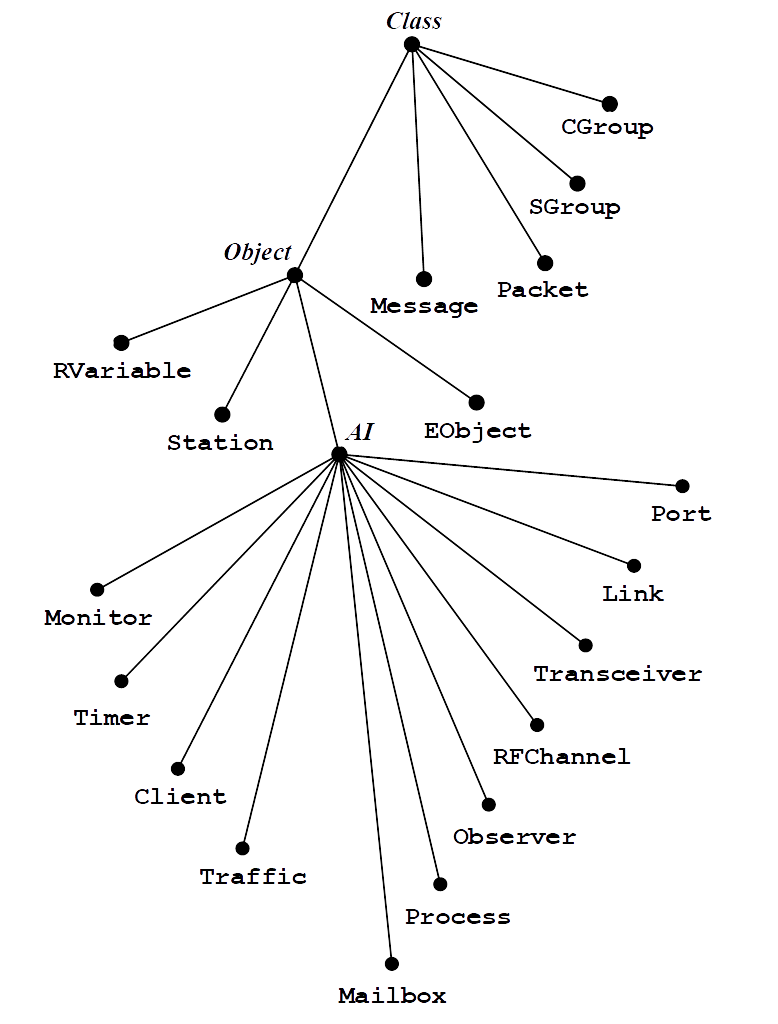
\includegraphics{FIGURES/hier.png}}
\caption{Hierarchy of user-visible compound types.}%
\label{ty_hi}
\end{center}
\end{figure}

All objects exhibiting dynamic behavior belong to type {\em Object}, which
is an internal type, not visible directly to the user.
Its role is to bind together its descendant types by furnishing them with a
small collection of common attributes and methods that each
{\em Object\/} must have.
Type {\tt EObject} can be used to prefix user-defined subtypes of {\em Object}.

The most relevant property of
an {\em Object\/} (or {\tt EObject}) is that it can be
{\em exposed}.
By {\em exposing\/} an object (see~\sect{rm_ex}) we mean presenting some
information related to the object in a standard way.
This information can be {\em printed}, i.e.,
included in the output file produced by the \smurph\ program,
or {\em displayed},
i.e., shown in a window on the terminal screen.

{\tt Timer} and {\tt Client} stand for specific objects rather than types.
These objects represent some important elements of the protocol environment
(see \sect{rm_pr_ai})
and are static, in the sense that they exist throughout the entire execution
of the protocol program.
Each of them occurs in exactly one copy.
Therefore,
the actual types of the above objects are uninteresting and are hidden from
the user.
Other {\em Objects\/} may exist in multiple copies; some of them may be
dynamically created and destroyed during a simulation run.

Generally, all objects rooted at {\tt AI\/} (which is another internal type
binding the so-called {\em activity interpreters\/})
are models of some entities belonging to the protocol environment.
They are responsible for modeling or perceiving
the flow of time, which is discussed in (\sect{rm_pr_ai}).

\subsection{{\em Object\/} naming}
\label{rm_st_on}

Each {\em Object\/} has a number of attributes that identify it from the outside
and a number of methods for accessing these attributes.
The reason for so many identifiers mostly results from the fact that the
dynamic display applet (\dsd)
responsible for exposing {\em Objects\/} on the screen (see
\sect{rm_ds}) must be
able to identify individual {\em Objects\/} and recognize some of their
general properties (see \sect{rm_ex}).

The following seven identification attributes are associated with each
{\em Object\/}:

\begin{itemize}
\item
the class identifier;
\item
the serial number;
\item
the type name;
\item
the standard name;
\item
the nickname;
\item
the base standard name;
\item
the output (print) name.
\end{itemize}

The {\em class identifier\/} of an {\em Object\/} is a number
identifying the base {\smurph}
type to which the {\em Object\/} belongs.
This attribute can be accessed by the parameter-less method
{\tt getClass}, e.g.,
{\tt\begin{tabbing}
12345678\=1234\=1234\=1234\=1234\=1234\=1234\=1234\=1234\kill
\> {\tt int  cl;}\\
\> {\tt ...}\\
\> {\tt cl = obj->getClass ();}
\end{tabbing}}
\noindent
which returns the following values:

\bigskip

\noindent
{\tt AIC\_timer~~~~~~~} if the object is the {\tt Timer} {\em AI}

\noindent
{\tt AIC\_client~~~~~~} if the object is the {\tt Client} {\em AI}

\noindent
{\tt AIC\_link~~~~~~~~} if the object is a {\tt Link}

\noindent
{\tt AIC\_port~~~~~~~~} if the object is a {\tt Port}

\noindent
{\tt AIC\_rfchannel~~~} if the object is an {\tt RFChannel}

\noindent
{\tt AIC\_transceiver~} if the object is a {\tt Transceiver}

\noindent
{\tt AIC\_traffic~~~~~} if the object is a {\tt Traffic}

\noindent
{\tt AIC\_mailbox~~~~~} if the object is a {\tt Mailbox}

\noindent
{\tt AIC\_process~~~~~} if the object is a {\tt Process}

\noindent
{\tt AIC\_observer~~~~} if the object is an {\tt Observer}

\noindent
{\tt AIC\_rvariable~~~} if the object is a {\tt RVariable}

\noindent
{\tt AIC\_station~~~~~} if the object is a {\tt Station}

\noindent
{\tt AIC\_eobject~~~~~} if the object is an {\tt EObject}

\bigskip

The {\em serial number\/}
of an {\em Object}, also called its {\tt Id}, tells apart
different {\em Objects\/} belonging to the same {\em class}.
This attribute is accessed by the method {\tt getId}, e.g.,
{\tt\begin{tabbing}
12345678\=1234\=1234\=1234\=1234\=1234\=1234\=1234\=1234\kill
 \> {\tt int  id;}\\
 \> {\tt ...}\\
 \> {\tt id = obj->getId ();}
\end{tabbing}}

With exception of {\tt Ports}, {\tt Transceivers} and {\tt Mailboxes},
all dynamically created
{\em Objects\/} are assigned their {\tt Id}s in the order of creation, such
that the first created {\em Object\/} in its {\em class} is numbered 0,
the second object is numbered 1, etc.
The numbering of {\tt Ports}, {\tt Transceivers} and {\tt Mailboxes}
is described in sections \ref{rm_to_po_cr}, \ref{rm_to_tr_cr} and
\ref{rm_mb_fi_dc}, respectively.
The {\tt Id} attribute of
the {\tt Timer} and the {\tt Client} (which never occur in multiple copies)
is equal to {\tt NONE} (--1).

The {\em type name\/} of an {\em Object\/} is a pointer to a character string
storing the textual name of the most restricted
type (C++ {\tt class}) to which the object belongs.
This pointer is returned by the method
{\tt getTName}, e.g.,
{\tt\begin{tabbing}
12345678\=1234\=1234\=1234\=1234\=1234\=1234\=1234\=1234\kill
 \> {\tt char *tn;}\\
 \> {\tt ...}\\
 \> {\tt tn = obj->getTName ();}
\end{tabbing}}

The purpose of the {\em standard name\/} is to identify exactly one
{\em Object}.
The standard name is a character string consisting of the object's
{\em type name\/} concatenated with the encoded {\em serial number}, e.g.\ 
{\tt MyProcess~245}.
The two parts are separated by exactly one space.
For a {\tt Port}, a {\tt Transceiver} and a station {\tt Mailbox}
(\sect{rm_mb_fi_dc}),
the standard name is built in a slightly more tricky way.
Namely, it contains as its part the standard name of the {\tt Station}
owning the object (see sections \ref{rm_to_po_cr}, \ref{rm_to_tr_cr},
\ref{rm_mb_fi_dc}).
For an object that always occurs in a single instance, the numerical part of
the standard name is absent, i.e., the standard names of the {\tt Timer}
and the {\tt Client} are just ``{\tt Timer}'' and ``{\tt Client},''
respectively.
The pointer to the object's standard name is returned by the method
{\tt getSName}, e.g.,
{\tt\begin{tabbing}
12345678\=1234\=1234\=1234\=1234\=1234\=1234\=1234\=1234\kill
 \> {\tt char *sn;}\\
 \> {\tt ...}\\
 \> {\tt sn = obj->getSName ();}
\end{tabbing}}

The {\em nickname\/} is an optional character string which can be assigned to
the object by the user.
This assignment is usually made when the object is created
(see \sect{rm_st_oc}).
The nickname pointer is returned by the method {\tt getNName}, e.g.,
{\tt\begin{tabbing}
12345678\=1234\=1234\=1234\=1234\=1234\=1234\=1234\=1234\kill
 \> {\tt char *nn;}\\
 \> {\tt ...}\\
 \> {\tt nn = obj->getNName ();}
\end{tabbing}}
\noindent
If no nickname has been assigned to the object, {\tt getNName} returns
{\tt NULL}.

The nickname is the only name that can be changed after it has been
assigned (all the other names are assigned by the system and they cannot
be changed).
The following method of {\em Object\/} can be used for this purpose:
\begin{verbatim}
        void setNName (const char *nn);
\end{verbatim}
where {\tt nn} is the assigned nickname.
If the {\em Object\/} didn't have a nickname, one is assigned by the method.
Otherwise, the previous nickname is discarded and the new one becomes
effective.

The {\em base standard name\/} is a character string
built similarly to the {\em standard name},
with the exception that the name of the base \smurph\ type from which the
type of the object has been derived is used instead of the object's
type name.
For example, assume that {\tt ms} points to an {\em Object\/} of
type {\tt MyStation} which has
been derived directly or indirectly from {\tt Station}.
The (regular) {\em standard name\/} of this object is
``{\tt MyStation~}{\em n}'',
whereas its base standard name is ``{\tt Station~}{\em n}''.
The pointer to the base standard name is returned by the method
{\tt getBName}, e.g.,
{\tt\begin{tabbing}
12345678\=1234\=1234\=1234\=1234\=1234\=1234\=1234\=1234\kill
 \> {\tt char *bn;}\\
 \> {\tt ...}\\
 \> {\tt bn = obj->getBName ();}
\end{tabbing}}
\noindent
The base standard names of objects that are direct instances of base types
are the same as their (regular) standard names.

The {\em output name\/} of an {\em Object\/} is a character string which is
the same as the {\em nickname}, if the nickname is defined; otherwise,
it is the same as the {\em standard name}.
When an {\em Object\/} is exposed {\em on paper\/} (see \sect{rm_ex}),
its output name is used as the default header of the exposure.
The method {\tt getOName} returns a pointer to the object's output name,
e.g.,
{\tt\begin{tabbing}
12345678\=1234\=1234\=1234\=1234\=1234\=1234\=1234\=1234\kill
 \> {\tt char *on;}\\
 \> {\tt ...}\\
 \> {\tt on = obj->getOName ();}
\end{tabbing}}

\noindent
{\bf Note:} The character strings returned by {\tt getSName},
{\tt getBName}, and {\tt getOName} are not constants.
Thus, if a string returned by one of these functions is to be stored, it
must be copied to a safe area.
On the other hand,
the strings pointed to by {\tt getTName} and {\tt getNName} are
constants and
they do not change for as long as the object in question is alive (or,
in the case of nickname, the name is not changed explicitly).

\subsection {Type derivation}
\label{rm_st_td}

Some of the types introduced in \sect{rm_st_th}
are templates that
can be used for creating problem-specific types defined by the user.
For example, type {\tt Process} can be viewed as a frame for defining
types representing processes to be run at stations.
One element of the process that must be provided by the user is a method
describing the process {\em code}, i.e., its behavior.
This element is specified in the user's part of the process type
definition.

\smurph\ provides a special way of deriving new types from the built-in
ones.
Here is the
simplest format of the operation that should be used for this purpose:
{\tt\begin{tabbing}
12345678\=1234\=1234\=1234\=1234\=1234\=1234\=1234\=1234\kill
\>{\em declarator\/} {\em typename\/} {\tt \{} \\
\> \>\ldots \\
\> \>{\em attributes and methods} \\
\> \>\ldots \\
\> {\tt \};}
\end{tabbing}}
\noindent
where {\em declarator\/} is a keyword corresponding to a base {\smurph}
type (\sect{rm_st_th}) and {\em typename\/} is the name of the
newly defined type.

\subsubsection*{Example}

\noindent
The following declaration:
\begin{verbatim}
        packet Token {
            int status;
        };
\end{verbatim}
defines a new packet type called {\tt Token}.
This type is built as an extension of the standard type {\tt Packet} and
contains one user-defined attribute---the integer variable {\tt status}.

The declarator keyword is obtained from the base \smurph\ type by changing
the first letter to the lower case.
The base types that can be extended this way are: {\tt Message},
{\tt Packet}, {\tt Traffic}, {\tt Station}, {\tt Link}, {\tt RFChannel},
{\tt Mailbox},
{\tt Process}, {\tt Observer}, and {\tt EObject}.

In most cases, it is possible to define the new type as a descendant of an
already defined type derived from the corresponding base type.
In such a case the name of the inherited type should appear after the new
type name preceded by a colon, i.e.,
{\tt\begin{tabbing}
12345678\=1234\=1234\=1234\=1234\=1234\=1234\=1234\=1234\kill
\>{\em declarator\/} {\em typename\/} {\tt :} {\em itypename\/} {\tt \{}\\
\> \>\ldots \\
\> \>{\em attributes and methods} \\
\> \>\ldots \\
\> {\tt \};}
\end{tabbing}}
\noindent
where {\tt itypename} identifies the inherited type, which must have been
declared previously with the same {\em declarator}.
In fact a declaration without {\em itypename\/} can be viewed as an
abbreviation for an equivalent declaration in which {\em itypename\/}
identifies the base type.
In particular, the previous declaration of type {\tt Token} is equivalent to
\begin{verbatim}
        packet Token : Packet {
            int status;
        };
\end{verbatim}

For the base types {\tt Traffic}, {\tt Process}, and {\tt Mailbox},
a subtype declaration (sections \ref{rm_cl_dt_tt}, \ref{rm_pr_dp},
\ref{rm_mb_fi_dc})
may optionally specify one or two {\em argument types}.
If present, these argument types are given in parentheses preceding the
opening brace.
Thus, the format of a subtype definition for these three base types is
{\tt\begin{tabbing}
12345678\=1234\=1234\=1234\=1234\=1234\=1234\=1234\=1234\kill
\>{\em declarator\/} {\em typename\/} {\tt :} {\em itypename\/} {\tt (}{\em argument types\/}{\tt )} {\tt \{} \\
\> \>\ldots \\
\> \>{\em attributes and methods} \\
\> \>\ldots \\
\> {\tt \};}
\end{tabbing}}
\noindent
where the parts ``{\tt :} {\em itypename\/}'' and ``{\tt (}{\em argument
types\/})'' are independently optional.

\subsubsection*{Examples}

\noindent
The following process type declaration:
{\tt\begin{tabbing}
12345678\=1234\=1234\=1234\=1234\=1234\=1234\=1234\=1234\kill
\>{\tt process Guardian (Node) \{}\\
\> \>\ldots \\
\> {\tt \};}
\end{tabbing}}
\noindent
defines a process type {\tt Guardian} descending directly from the base type
{\tt Process}.
The argument type should be a defined (or announced---see \sect{rm_st_an})
station type;
it tells the type of stations that will be running processes of type
{\tt Guardian}.

With the following declaration:
{\tt\begin{tabbing}
12345678\=1234\=1234\=1234\=1234\=1234\=1234\=1234\=1234\kill
\>{\tt process SpecializedGuardian : Guardian (MyNode) \{}\\
\> \>\ldots \\
\> {\tt \};}
\end{tabbing}}
\noindent
you can build a subtype of {\tt Guardian}.
Processes of this type will be owned by stations of type {\tt MyNode}.

\medskip

\noindent
The exact semantics of the \smurph\ type extension operations
will be described individually for each extensible base type.
Every such operation is expanded into the definition of a class
derived either from the corresponding base type or from
the specified supertype.
Some standard attributes (mostly invisible to the user) are automatically
associated with this class.
These attributes will be used by \smurph\ to keep track of what happens
to the objects created from the defined type.

The inherited supertype class is made {\tt public} in the subclass.
Following the opening brace of the type definition, the user can define
attributes and methods of the new type.
By default, all these attributes are {\tt public}.
The C++ keywords
{\tt private}, {\tt protected}, and {\tt public} can be used to associate
specific access rights with user-defined attributes.

\subsection {Multiple inheritance}
\label{rm_st_mi}

Sometimes it may be convenient to define a \smurph\ subtype as a direct
descendant of more than one supertype.
This may be especially useful when creating libraries of types.
The standard concept of {\em multiple inheritance\/} (present in C++)
is more or less naturally applicable in such situations; however,
\smurph\ adds to the issue a specific flavor resulting from the
following two problems:
\begin{itemize}
\item
It is meaningless to define types derived simultaneously
from different base types.
Thus there should be a way of controlling whether a \smurph\ type extension
makes sense.
\item
An object of a type derived from multiple supertypes must have exactly one
frame of its base type.
\end{itemize}

The first fact is rather obvious: what would it mean to have an object that is
both a {\tt Station} and a {\tt Message} at the same time?
The second fact is a consequence of the way in which objects derived from the
base \smurph\ types are handled by the kernel.
Internally, each such object is represented by various pointers and tags
kept in its base type part.
Having two or more copies of this part, besides wasting a substantial amount of
space, would have the disastrous effect of
perceiving a single object as multiple objects.

In C++ it is possible to indicate that the frame corresponding to a given
class occurs exactly once in the object frame, even if the class occurs
several times in the object's type derivation.
This is achieved by declaring the class as {\tt virtual} in the derivation
sequence.
Thus, one possible solution to be adopted in \smurph\ would be to force
each base type to occur as {\tt virtual} in the derivation list of a
user-defined type.
This solution, however, would be quite costly.
To make it work, one should always have to make the base types virtual, even
if no multiple inheritance were used.\footnote {Note that the \smurph\ program
may be contained in several files and the fact that no multiple inheritance is
used in one file does not preclude it from being used in another one.}
This would be expensive because the frame of a virtual subclass is referenced
via a pointer, which substantially increases the cost of such a reference.
Therefore, another solution has been adopted.

If the name of a newly defined \smurph\ supertype is followed by
{\tt virtual}, e.g.,
{\tt\begin{tabbing}
12345678\=1234\=1234\=1234\=1234\=1234\=1234\=1234\=1234\kill
\>{\tt station VirPart virtual \{}\\
\> \>\ldots \\
\> {\tt \};}
\end{tabbing}}
\noindent
it means that formally the type belongs to the corresponding base type,
but the frame of the base type will not be attached to the type's frame.

The {\em itypename\/} part of a \smurph\ subtype definition
(\sect{rm_st_td}) may contain a sequence of type names separated by commas,
e.g.,
{\tt\begin{tabbing}
12345678\=1234\=1234\=1234\=1234\=1234\=1234\=1234\=1234\kill
\>{\tt packet DToken : AToken, BToken, CToken \{}\\
\> \>\ldots \\
\> {\tt \};}
\end{tabbing}}
This sequence represents the inheritance list of the defined subtype.
The following rules must be obeyed:
\begin{itemize}
\item
The inheritance list may contain at most one non-virtual type name (in the
sense described above).
If a non-virtual type name is present, it must appear first on the list.
\item
If the name of the defined type is followed by {\tt virtual} (this keyword
must precede the colon), the inheritance list must not include a
non-virtual type.
\item
If the inheritance list contains virtual types only, but the keyword
{\tt virtual} does not follow the name of the defined type, the defined
type {\bf is not virtual}, i.e., the base type is implicitly added to
the inheritance sequence (as the first element).
Thus only the types explicitly declared as {\tt virtual} are made {\tt virtual}.
\end{itemize}

One disadvantage of this solution is that a virtual (in the \smurph\ sense)
type cannot reference attributes of the base type.
This is not a big problem, as very few of these attributes may be of
interest to the user.
Virtual functions can be used to overcome this difficulty, if it ever
causes a problem.

\subsection{Abstract types}
\label{rm_st_ab}

A \smurph\ type can be explicitly declared as incomplete (and thus unusable
for creating objects) by putting the keyword {\tt abstract} into its
declaration, e.g.,
{\tt\begin{tabbing}
12345678\=1234\=1234\=1234\=1234\=1234\=1234\=1234\=1234\kill
\>{\tt traffic MyTrafficInterface abstract \{}\\
\> \>\ldots \\
\> {\tt \};}
\end{tabbing}}
\noindent
An abstract type can be derived from other (possibly non-abstract) types, but
it cannot be virtual (\sect{rm_st_mi}).
Thus, the keywords {\tt abstract} and {\tt virtual} cannot occur in the same
type declaration.

If an abstract type is derived from other types, then those types must be
listed after a colon following the {\tt abstract} keyword, e.g.,
{\tt\begin{tabbing}
12345678\=1234\=1234\=1234\=1234\=1234\=1234\=1234\=1234\kill
\>{\tt traffic MyTrafficInterface abstract : XTraffic (Msg, Pkt) \{}\\
\> \>\ldots \\
\> {\tt \};}
\end{tabbing}}

Essentially, an abstract type has all the features of a regular
type, except that {\tt create} for such a type (\sect{rm_st_oc}) is illegal.
Moreover, a type {\em must\/} be declared {\tt abstract} if it declares
abstract virtual methods.
For example, this declaration:
{\tt\begin{tabbing}
12345678\=1234\=1234\=1234\=1234\=1234\=1234\=1234\=1234\kill
\>{\tt traffic MyTrafficInterface abstract (Msg, Pkt) \{}\\
\> \>{\tt virtual Boolean check\_it (Pkt *p) = 0;} \\
\> \>\ldots \\
\> {\tt \};}
\end{tabbing}}
\noindent
would trigger errors if the {\tt abstract} keyword following the traffic type
name were absent.

\subsection {Announcing types}
\label{rm_st_an}

A \smurph\ subtype can be announced before it is actually defined.
This may be needed occasionally, if the name of the type is required
(e.g.,
as an {\em argument type\/}---\sect{rm_st_td}) before the full definition
can take place.
The following type declaration format is used for this purpose:
{\tt\begin{tabbing}
12345678\=1234\=1234\=1234\=1234\=1234\=1234\=1234\=1234\kill
\>{\em declarator\/} {\em typename\/}{\tt ;}
\end{tabbing}}
\noindent
where {\em declarator\/} has the same meaning as in \sect{rm_st_td}.
The type name can be optionally followed by {\tt virtual} in which case
the type is announced as virtual in the sense of \sect{rm_st_mi}.
Note that a full type definition must precede the usage of this type in the
inheritance sequence of another type.

\subsection {Subtypes with empty local attribute lists}
\label{rm_st_ea}

There are many cases when the local attribute list of a \smurph\ subtype
is empty, e.g.,
\begin{verbatim}
        traffic MyTPattern (MyMType, MyPType) { };
\end{verbatim}
This situation occurs most often for traffic patterns (subtypes of
{\tt Traffic}) and mailboxes (subtypes of {\tt Mailbox}).
In such a case, it is legal to skip the empty pair of braces, provided that
the new type declaration cannot be confused with a type
announcement (\sect{rm_st_an}).
In particular, the above definition of {\tt MyTPattern} can be shortened to
\begin{verbatim}
        traffic MyTPattern (MyMType, MyPType);
\end{verbatim}
as, due to the presence of the argument types, it does not look like a type
announcement.
On the other hand, in the declaration
\begin{verbatim}
        packet MyPType { };
\end{verbatim}
the empty pair of braces cannot be omitted, as otherwise the declaration would
just announce the new packet type without actually defining it.
Generally, an abbreviated type declaration (without braces) is treated as
an actual type definition rather than an announcement, if at least one of
the following conditions is true:
\begin{itemize}
\item
the declaration contains argument types
\item
the declaration specifies explicitly the supertype
\end{itemize}
Thus, the above declaration of {\tt MyPType} can be written equivalently as
\begin{verbatim}
        packet MyPType : Packet;
\end{verbatim}
which, however, is hardly an abbreviation.
On the other hand, the most common cases when the attribute list of a newly
defined type is empty deal with subtypes of {\tt Traffic} and {\tt Mailbox}
and then argument types are usually present.

\subsection{Object creation and destruction}
\label{rm_st_oc}

If an object belonging to a base \smurph\ type or its derived type
is to be created explicitly,
the following operation must be used:
{\tt\begin{tabbing}
12345678\=1234\=1234\=1234\=1234\=1234\=1234\=1234\=1234\kill
\>{\tt obj = create {\em typename\/} (} {\em setup args\/} {\tt );} \\
\end{tabbing}}
\noindent
where {\em typename\/} is the name of the object's type.
The arguments in parentheses are passed to the object's
{\tt setup} method.
If the object has no setup method, or the list of arguments of this method is
empty, the part in parentheses does not occur (the empty parentheses can be
skipped as well).
The operation returns a pointer to the newly created object.

The purpose of the {\tt setup} method is to perform object
initialization.
If it is needed, it should be declared as
{\tt\begin{tabbing}
12345678\=1234\=1234\=1234\=1234\=1234\=1234\=1234\=1234\kill
\>{\tt void setup (}\ldots {\tt );}
\end{tabbing}}
\noindent
within the object type definition.
Argument-less C++ constructors can also be used in user-defined derived
{\smurph}
types; however, there is no way to define and invoke upon object
creation a constructor with arguments.
The role of such a constructor is played by {\tt setup}.
Non-extensible types (\sect{rm_st_td}) and types that need not be
extended define appropriate standard/default {\tt setup} methods.
Their arguments and semantics will be discussed separately for each 
basic type.

It is possible to assign a nickname (see \sect{rm_st_on})
to the created object.
The following version of create can be used for this purpose:
{\tt\begin{tabbing}
12345678\=1234\=1234\=1234\=1234\=1234\=1234\=1234\=1234\kill
\>{\tt obj = create {\em typename}, {\em nickname}, (} {\em setup args\/} {\tt );}
\end{tabbing}}
\noindent
where {\em nickname\/} is an expression that should evaluate to a
character pointer.
The string pointed to by this expression will be duplicated and used
as the object's nickname.
If the {\em setup args\/} part does not occur, the second comma together
with the parentheses may be omitted.

\medskip
\noindent
{\bf Note:} The comma following {\em nickname\/} is needed (it
is not a mistake).

\medskip
\noindent

The {\em typename\/} keyword (in both versions of {\tt create}) can be
optionally preceded by an expression enclosed in parentheses, i.e.,
{\tt\begin{tabbing}
12345678\=1234\=1234\=1234\=1234\=1234\=1234\=1234\=1234\kill
\>{\tt obj = create ({\em expr\/}) {\em typename\/} (} {\em setup args\/} {\tt );} \\
\end{tabbing}}
or
{\tt\begin{tabbing}
12345678\=1234\=1234\=1234\=1234\=1234\=1234\=1234\=1234\kill
\>{\tt obj = create ({\em expr\/}) {\em typename}, {\em nickname}, (} {\em setup args\/} {\tt );}
\end{tabbing}}
\noindent
where {\em expr\/} must be either of type {\tt int} (in which case it will be
interpreted as a station {\tt Id})
or a pointer to an object belonging to a {\tt Station} subtype.
It identifies the
station in the context of which the new object is to be created and is
relevant for some object types only (e.g., see \sect{rm_pr_ct}).
The switchover to the context of the indicated station
only affects the {\tt create} operation, as well as any operations triggered
by it (e.g., the execution of the created object's setup method).

Objects belonging to types {\tt SGroup}, {\tt CGroup}, {\tt Station},
{\tt Traffic}, {\tt Link}, {\tt RFChannel}, {\tt Mailbox},\footnote{This only
concerns those mailboxes that are owned by stations.
Mailboxes owned by processes can be destroyed (see \sect{rm_mb_fi_dc}).}
{\tt Port}, and
{\tt Transceiver} can only be created and never explicitly destroyed.
Other dynamically created
objects can be destroyed with the standard C++ operator {\tt delete}.

User-defined subtypes of {\em Object\/} must belong to type {\tt EObject}, i.e.,
be actually declared as derivatives of {\tt EObject} or its descendants.
A declaration of such a subtype should start with the keyword {\tt eobject}
and obey the rules listed in sections \ref{rm_st_td} and \ref{rm_st_mi}.
An {\tt EObject} subtype
may declare a {\tt setup} method (or a number of such methods).
Object instances of {\tt EObject} subtypes should be generated
by {\tt create} and deallocated by {\tt delete}.

{\tt Id} attributes of {\tt EObjects} reflect their order of
creation starting from 0.
This numbering is common for all subtypes of {\tt EObject}.

\medskip

\noindent
{\bf Note:} it is illegal to {\tt create} an object of a virtual type
(\sect{rm_st_mi}).

%%%@@@-- defin.tex
\section{Defining system geometry}
\label{rm_to}

The logical structure of the modeled/controlled
system (we shall call it a network), although static from the viewpoint
of the protocol program, is defined dynamically by explicit object creation
and calls to some functions and methods.
As perceived by \smurph, a network consists of {\em stations\/} which are
conceptually the processing units of the network.
A station can be viewed as a hardware
(a parallel computer) that runs a collection of {\em processes}.
These processes implement a part of the protocol program which is run by
the entire network.

Sometimes (especially in network simulators) stations
are interconnected via {\em links\/} or/and {\em radio channels}.
Links, represented by type {\tt Link} (and its few built-in variants),
are models of
simple communication channels that can be implemented in real life
on the basis of some broadcast-type communication media, e.g.,
a piece of wire, a coaxial cable, an optical fiber, or even a wireless link
(although {\tt RFChannel}s are generally more useful for that purpose).

Stations are interfaced to links via {\em ports},
which can be viewed as some specific points (taps) on the links
that the stations may use to send and receive information.
Links introduce propagation delays; therefore, one application of a link
in a control program is to implement a delayed communication between a pair
of stations.

Radio channels, represented by objects of type {\tt RFChannel}, are similar
to links, excepts that they allow for more dynamic (in particular mobile)
configurations of stations interconnected by them.
Also, radio channels are more open-ended: they come with hooks whereby users
can describe (program)
their favorite characteristics related to
transmission power, receiver gain (sensitivity), transmission
range, signal attenuation, interference, i.e., all the interesting attributes
of real-life radio channels relevant from the viewpoint of modeling signal
propagation and packet reception.
Owing to the large and unforeseeable set of possible channel models that
people may want to plug into \smurph\ simulators, the package does not
presume any built-in characteristics, except for the timing of signals
according to the (Euclidean) distance between the concerned points.

The radio channel equivalent of a port is called a {\em transceiver}.
Similar to a port, it represents an interface of a station to a
radio channel.
Multiple (independent) radio channels can coexists within a single network
model.
Also, links can coexist with radio channels.
Thus, hybrid networks can be modeled in \smurph.

\subsection{Stations}
\label{rm_to_st}

A station is an object belonging to a type derived from {\tt Station}
(see \sect{rm_st_th}).
It is possible to create a station belonging directly to type
{\tt Station}, but such a station is not very useful.

The standard type {\tt Station} defines only two attributes visible to the
user, which are practically never accessed directly.
These attributes describe the queues of {\em messages\/} awaiting transmission
at the station and are discussed in \sect{rm_cl_mq}.

\subsubsection{Defining station types}
\label{rm_to_st_ds}

The definition of a new station type starts with the keyword {\tt station}
and obeys the rules listed in sections
\ref{rm_st_td} and \ref{rm_st_mi}.
The {\tt setup} method for a station type needs only be defined if the type
declares attributes that must be initialized when a station
object of this type is created.

\subsubsection*{Examples}

\noindent
The following declaration:
\begin{verbatim}
        station Hub {
            Port **Connections;
            int  Status;
            void setup () { Status = IDLE; };
        };
\end{verbatim}
defines a new station type called {\tt Hub} derived directly from
{\tt Station}, with two attributes: an array of pointers to
ports and an integer
variable.
When a {\tt Hub} object is created, the {\tt Status} attribute will
be set to {\tt IDLE}.
The array of port pointers is not initialized in the {\tt setup} method, so,
presumably, it will be created outside the object.

The {\tt Hub} type defined above can be used to derive another
station type, e.g.,
\begin{verbatim}
        station SuperHub : Hub {
            TIME *TransferTimes;
            void setup (int hsize) {
                Hub::setup ();
                TransferTimes = new TIME [hsize];
            };
        };
\end{verbatim}

The {\tt SuperHub} type inherits all attributes from {\tt Hub} and declares
one private attribute---an array of {\tt TIME} values.
The {\tt setup} method has now one argument.
Note the call to the {\tt setup} method of the supertype---to initialize
the {\tt Status} attribute.

Stations are the most natural candidates to be defined from virtual supertypes,
according to the rules described in \sect{rm_st_mi}.
For example, consider the following declaration:
\begin{verbatim}
        station TwoBusInterface virtual {
            Port *Bus0Port, *Bus1Port;
            void setup (RATE tr) {
                Bus0Port = create Port (tr);
                Bus1Port = create Port (tr);
            };
        };
\end{verbatim}
which defines a station component.
This component consists of two ports which are created by the {\tt setup}
method (the details are explained in \sect{rm_to_po_cr}).
The two ports may provide a station interface to a two-bus network without
specifying any other details of the station architecture.
The next declaration
\begin{verbatim}
        station ThreeBuffers virtual {
            Packet Buf1, Buf2, Buf3;
        };
\end{verbatim}
can be viewed as a description of a {\tt Client} interface (\sect{rm_cl_pb})
consisting of three packet buffers.
The two interfaces can be used together in a single derived
definition, e.g.,
\begin{verbatim}
        station MyStationType : TwoBusInterface, ThreeBuffers {
            RVariable *PacketDelay;
            void setup () {
                RATE MyXRate;
                PacketDelay = create RVariable;
                readIn (MyXRate);
                TwoBusInterface::setup (MyXRate);
            };
        };
\end{verbatim}
as independent building blocks for a complete (non-virtual) station type.

\subsubsection{Creating station objects}
\label{rm_to_st_cs}

Given a station type, a station object is built by executing {\tt create}
(see~\sect{rm_st_oc}).
The serial number (the {\tt Id} attribute---see \sect{rm_st_on}) of a
station object reflects its creation order.
The first-created station is assigned number 0, the second one is numbered 1,
etc.
The global read-only variable {\tt NStations} of type {\tt int} contains
the number of all stations that have been created so far.

As the system geometry must be completely determined before the protocol
execution is started, it is illegal to create new stations after starting
the protocol.
Also, once created, a station can never be destroyed.
At first sight, this may look like a limitation reducing the expressing power
for the model's dynamics, e.g., in ad-hoc wireless networks, where one may
want to study mobility and varying populations of stations that come and go.
Note, however, that a station's behavior can be arbitrarily dynamic and
independent of the behavior of other stations.
Station can remain dormant, then wake up, then become dormant again.
In a wireless network, they can also change their locations, move out of range,
and so on.
The operation of pre-building the model's virtual hardware should be viewed as
creating a virtual universe.
Once created and set in motion, the ``substance'' of this universe is not
allowed to change, but it can behave in a highly dynamic way.

There exists one special (and typically inconspicuous) station,
which is created automatically before anything else.
Its purpose is to run a few internal processes
of \smurph\ and also the user's {\tt Root} process (see \sect{rm_pr_or}).
This station is pointed to by the global variable {\tt System} whose
type (a subtype of {\tt Station}) is hidden from the user.
The {\tt Id} attribute of the {\tt System} station is {\tt NONE} and its
{\em type name\/} is {\tt SYSTEM}.

Sometimes it is convenient and natural to reference a station by its
serial number, i.e., the {\tt Id} attribute, rather than the object pointer.
For example, station numbers are used to identify senders and receivers
of messages and packets (see \sect{rm_cl_mp}).
Quite often, especially at the initialization stage, one would like to perform
some operation(s) for all stations, or perhaps for their large subset.
In such a case, it may be natural to use a loop of the following form:
{\tt\begin{tabbing}
12345678\=1234\=1234\=1234\=1234\=1234\=1234\=1234\=1234\kill
 \> {\tt for (int i = 0; i < NStations; i++) } \ldots
\end{tabbing}}
To make such operations possible,
the following function\footnote{Implemented as a macro.} converts a
station {\tt Id} into the pointer to the station object:
\begin{verbatim}
        Station  *idToStation (int id);
\end{verbatim}
The function checks whether the argument is a legal station number and, if it
is not the case, the execution is aborted with a pertinent error message.

\medskip

\noindent
{\bf Note:} For symmetry, the following macro looks like a function
that returns the {\tt Id} attribute
of a station (or any {\em Object\/}) whose pointer is specified as the
argument:
\begin{verbatim}
        int  ident (Object *a);
\end{verbatim}
This macro expands into a call to {\tt getId} (see \sect{rm_st_on}).

\subsubsection{Current station}
\label{rm_to_st_cu}

At any moment when a protocol thread (process) is run,
as well as during the network initialization phase,
it is known which station is the one that is currently {\em active}.
One can say that anything that ever happens in a \smurph\ program
always happens within the context of some station.
This (current) station is pointed to by the global variable {\tt TheStation}
of type {\tt Station}, which belongs to the so-called
{\em process environment\/} (see \sect{rm_pr_en}).
When \smurph\ starts, and the user program is given control for the first time,
{\tt TheStation} points to the {\tt System} station.
Then, whenever a new user-defined station is created,
{\tt TheStation} points to that last created station.
Many other objects that get created along the way (e.g.,
ports, transceivers, processes) are supposed to belong (be owned) by
specific stations; thus, they are assigned by default to the station pointed
to by {\tt TheStation} at the moment of their creation.
This means that sometimes it may
make sense to set {\tt TheStation} explicitly---to
assume the context of a specific station and make sure that the object
(or objects) subsequently created will be assigned to the right owner.
There exists a version of {\tt create} with an extra argument specifying the
station that should be made current (assigned to {\tt TheStation})
before the actual object creation (see \sect{rm_st_oc}).

\subsection{Links}
\label{rm_to_li}

Links are objects belonging to type {\tt Link}, which exists in four standard
subtypes: {\tt BLink}, {\tt ULink}, {\tt PLink}, and {\tt CLink}.
The primary purpose of a link is to model a simple wired
communication channel.
Two types of wired channel models, broadcast and unidirectional links,
are built into \smurph, each of the two types occurring in two marginally
different flavors.

\subsubsection{Propagation of information in links}
\label{rm_to_li_pr}

A broadcast link is a uniform information passing medium with the
property that a signal entered into any port connected to the link
reaches all other ports of the link in due time.
A typical real-life example of the broadcast link model is a piece of
wire (e.g., a coaxial cable).
In a unidirectional link, information travels in one direction only: for any two
ports {\em A\/} and {\rm B\/} on such a link, there is either a path from {\em A\/} to {\rm B\/} or
from {\rm B\/} to {\em A\/}, but never both.
A typical physical implementation of a unidirectional link is a single,
segmented fiber-optic channel.

Irrespective of the link type, the actual geometry of the link is described
by the {\em link distance matrix\/} which specifies the propagation distance
between each pair of ports connected to the link.
The propagation distance from port {\em A\/} to port {\rm B\/} is equal to the (integer)
number of {\em ITU\/}s required to propagate information from {\em A\/} to {\em B}.
If an activity, typically a packet transmission (see~\sect{rm_po_ac_st}),
is started on port {\em A\/} at time {\em t},
that activity will arrive on port {\rm B\/} at time
{\em t~+~D[A,B]}, where
{\em D\/} is the link distance matrix.
For a broadcast bidirectional link (types {\tt BLink} and {\tt CLink}),
the propagation distance is independent of the direction, i.e.,
the propagation distance
from {\em A\/} to {\rm B\/} is the same as the propagation distance from {\rm B\/} to {\em A}.
In other words, the distance matrix of a broadcast link is symmetric.

For a unidirectional link (types {\tt ULink} and {\tt PLink}),
the order in which particular ports have been connected to the link (see
\sect{rm_to_po_co})
determines the propagation direction, i.e.,
if port {\em A\/} was connected earlier than {\rm B\/} (we assume that the two ports belong
to the same link), then signals can propagate
from {\em A\/} to {\em B}, but not from {\rm B\/} to {\em A}.
It means that an activity inserted at time {\em t\/} into {\em A\/} will reach {\rm B\/} at
time {\em t~+~D[A,B]\/}---as for a broadcast link, but no activity
inserted into {\rm B\/} will ever arrive at {\em A}.
Thus, the distance matrix of a unidirectional link is
triangular.\footnote{In fact, distance matrices do not occur explicitly:
they are
distributed into {\em distance vectors\/} associated with ports rather
than links.}

If a unidirectional link has a strictly linear topology, i.e.,
for every three ports {\em A}, {\em B}, {\em C\/} created in the listed order
{\em D[A,C]~=~D[A,B]~+~D[B,C]},
the link should be declared as a {\tt PLink}, which type
can only be used to represent strictly linear, unidirectional links.
Semantically, there is no difference between types {\tt PLink} and {\tt ULink}
used to represent such a link; however, the {\tt PLink} representation is
usually much more efficient, especially when the link is very long
compared to the duration of a typical activity inserted into it.

More information about links is contained in \sect{rm_po_wr} where
the concept of a collision is discussed.
For the purpose of this section, it is enough to say that there are two
different methods of recognizing collisions in a bidirectional
link.
The existence of two types for representing a bidirectional link is a
direct consequence of this fact.
The two types {\tt BLink} and {\tt CLink} are semantically identical,
except for the difference in interpreting collisions.
Type {\tt BLink} is equivalent to the simplest generic link type {\tt Link}.

\subsubsection{Creating links}
\label{rm_to_li_cr}

Link objects are seldom, if ever, referenced directly by the protocol
program, with exception of the network creation phase when the links must
be built and configured.
It is technically possible (but seldom useful)
to define a new link type with the following operation:
{\tt\begin{tabbing}
12345678\=1234\=1234\=1234\=1234\=1234\=1234\=1234\=1234\kill
\>{\tt link }{\em newtypename\/} {\tt : }{\em oldtypename\/} {\tt \{} \\
\> \>\ldots \\
\> {\tt \};}
\end{tabbing}}
One use for this possibility is to augment the standard
performance measuring link methods
by user-defined functions (see \sect{rm_pm_lk}), or to declare a
non-standard link method for generating erroneous packets
(\sect{rm_po_fl}).
If the {\em oldtypename\/} part is absent,
the new link type is derived directly from {\tt Link}.

A link object is created by {\tt create}---in a way similar to
any other {\em Object\/} (see \sect{rm_st_oc}).
The standard link {\tt setup} method is declared with the following header
(the same for all link types):
\begin{verbatim}
        void setup (Long np, RATE r, TIME lin, int spf);
\end{verbatim}
The first argument, {\tt np}, specifies the number
of ports that will be connected to the link.
The second argument, {\tt r}, provides the default transmission rate for a
port connected to the link.
That rate will be assigned to every port connected to the link that doesn't
directly specify a transmission rate at its creation (\sect{rm_to_po_cr}).
The third argument, {\tt lin}, gives the link {\em linger\/}
(or {\em archival\/})
interval in {\em ITU\/}s.
The linger time determines for how long descriptions of activities that
have formally disappeared from the link are to be kept in the link
data base (see \sect{rm_po_ac_pr}).
Note that the default value of the linger attribute is zero.
With this setting,
any activity inserted into the link will be removed
at the time when its last bit passes the most distant port,
as seen from the port of its insertion.

The linger attribute can also be set dynamically,
after the link has been created, by invoking this {\tt Link} method:
\begin{verbatim}
        void setPurgeDelay (TIME lin);
\end{verbatim}

The last argument of the {\tt Link} {\tt setup} method
indicates whether standard performance measures
are to be calculated for the link.
{\tt ON} (1) means that the standard performance measures will be
computed; {\tt OFF} (0) turns them off.

There is an alternative (shortcut) setup method for {\tt Link} declared as:
\begin{verbatim}
        void setup (Long np, TIME lin = TIME_0, int spf = ON);
\end{verbatim}
\noindent
which translates into this call:
\begin{verbatim}
        setup (np, RATE_0, lin, spf);
\end{verbatim}
\noindent
and basically ignores the default port rate argument setting it to zero (note that such a rate is not usable for transmission---\sect{rm_to_po_cr}).
Thus, ports are expected to take care of their transmission
rates all by themselves. 

With the two setup variants for {\tt Link}, the {\tt create} operation for a link expects at least one and at most four setup arguments.

\medskip

\noindent
{\bf Note:} If you have provided non-standard performance measuring
methods for a link (see \sect{rm_pm_lk}), they will be called even if
the link has been created with {\tt spf = OFF}.

\medskip

A link created according to the above rules is a raw link, in the sense that
it is not configured into the network.
The value of {\tt np} specifies only the number of slots for ports that
will be eventually connected to the link,
but these ports are neither created nor anything is said
about their geometric distribution.
In fact, nothing is known at this moment
about the geometry of the link: as we said
in \sect{rm_to_li_pr}, this geometry is determined by distances
between pairs of ports, and these distances must be assigned
explicitly (\sect{rm_to_po_se}).

The {\tt Id} attributes of links (and also their standard names---see
\sect{rm_st_on}) reflect the order in which the links have been created.
The first created link gets number 0, the second link---number 1, etc., until
{\em n\/}--1, where {\em n\/} is the total number of links in the network.
In many cases when a link is to be referenced, it is possible to use either
a pointer to the link object or the link number (its {\tt Id} attribute).
The following function:
\begin{verbatim}
        Link *idToLink (Long id);
\end{verbatim}
converts a numerical link {\tt Id} to the Link pointer.
The global variable {\tt NLinks} of type {\tt int} stores the number of
all links created so far.

\subsection{Ports}
\label{rm_to_po}

Ports are objects of the
standard type {\tt Port}, which is not extensible by the user.
Therefore, there is no {\tt port} operation that would declare a {\tt Port}
subtype.

\subsubsection{Creating ports}
\label{rm_to_po_cr}

There are two ways to create a port.
One is to use the standard {\tt create} operation
(see \sect{rm_st_oc}).
The port {\tt setup} method for this occasion is declared as follows:
\begin{verbatim}
        void setup (RATE rate = RATE_inf);
\end{verbatim}
where the optional argument defines the port transmission rate (attribute
{\tt XRate}) as the
number of {\em ITU\/}s required to insert a single bit into the port.
This attribute is relevant if the port will ever
be used for {\em transmission\/}
(see \sect{rm_po_ac}) and determines the amount of time
required to transmit a packet through the port.

The default value, {\tt RATE\_inf}, assumed if you don't explicity specify a
transmission rate at the port's creation, is interpreted as ``none'' and
means that the default transmission rate associated with the link
(\sect{rm_to_li_cr}) should be used for the port.
That rate will be copied by the port from the link at the moment when
the port gets
{\em connected\/} to the link (\sect{rm_to_po_co}).
If nothing is ever transmitted via the port, i.e., the port
is used for reception only, its transmission rate is irrelevant.

Ports are naturally associated with stations and links.
From the viewpoint of the protocol program, the association of a port
with a station is more important than its association with a link, as
links are not perceived directly by the protocol processes.
Therefore, a port can be declared statically within a
station type and then created automatically when the station is created, i.e.,
{\tt\begin{tabbing}
12345678\=1234\=1234\=1234\=1234\=1234\=1234\=1234\=1234\kill
\>{\tt Port }{\em portname\/}{\tt ;}
\end{tabbing}}
\noindent
Note that such a port is not explicitly assigned a transmission rate (it
will inherit the rate from the link at the moment of
connection---\sect{rm_to_po_co}).
Note that the rate can also be specified later (and redefined at any time)
by the {\tt setRate} method of {\tt Port}.
For illustration, in the following code:
\begin{verbatim}
        station BusStation {
         ...
          Port P;
         ...
          void setup () {
           ...
            P.setXRate (myXRate);
            P.setNName (myNickname);
           ...
          };
         ...
        };
\end{verbatim}
\noindent
the statically declared port {\tt P} is assigned a transmission rate as well
as a nickname in the setup method of its station.
Note that it doesn't matter whether the port is connected to a link
at the moment
or not, as long as the specified rate is not {\tt RATE\_inf}.
Any non-void (different from {\tt RATE\_inf}) rate explicitly
assigned to a port always takes precedence over any default rate
defined by the link.

In addition to setting the transmission rate of its port, {\tt setXRate}
returns the previous setting of the rate.
The method is declared with the following header:
\begin{verbatim}
        RATE setXRate (RATE r = RATE_inf);
\end{verbatim}
\noindent
When called with the void rate {\tt RATE\_inf}
(or with no argument at all), the method will
cause the port to be assigned the default transmission rate of its
link, but that will only work if the port is already connected---\sect{rm_to_po_co}).
Any other value is interpreted as the port's new, private, and specific
transmission rate.

This method:
\begin{verbatim}
        RATE getXRate ();
\end{verbatim}
\noindent
just returns the current setting of the transmission rate.
As a general rule, most ``set'' methods have their ``get'' counterparts.

\medskip

No matter which way a port has been created,
from the beginning of its existence it is associated with a specific station.
If the port has been declared statically
as a station attribute, the situation is clear:
as soon as the station has been created, the port comes into existence and
is automatically assigned to the station.
When a port is created by {\tt create}, it is assigned to
the {\em current\/} station pointed to by the environment
variable {\tt TheStation} (see \sect{rm_to_st_cu}).

All ports belonging to one station are assigned numerical identifiers starting
from 0 up to {\em n\/}--1, where {\em n\/} is the total number of ports owned by the
station.
This numbering of ports reflects the order of their
creation and is used to construct the
{\tt Id} attributes of ports (\sect{rm_st_on}).
Namely, the {\tt Id} attribute of a port consists of two numbers: the {\tt Id}
attribute of the station owning the port and the station-relative port
number determined by its creation order.
These numbers are shown separately in the port's standard name
(see \sect{rm_st_on}) which has the following format:
{\tt\begin{tabbing}
12345678\=1234\=1234\=1234\=1234\=1234\=1234\=1234\=1234\kill
\>{\tt Port }{\em pid\/}~{\tt at}~{\em stname}
\end{tabbing}}
\noindent
where {\em pid\/} is the relative number of the port at its station, and
{\em stname\/} is the standard name of the station owning the port (note that
it includes the station's {\tt Id}).

The following {\tt Station} method:
\begin{verbatim}
        Port *idToPort (int id);
\end{verbatim}
can be used to convert the numerical station-relative port identifier into
a pointer to the port object.
An alternative way to do the same is to call a global function declared
exactly as the above method, which assumes that the station in question is
pointed to by {\tt TheStation}.

The following two {\tt Port} methods:
\begin{verbatim}
        int getSID ();
        int getYID ();
\end{verbatim}
return the numerical {\tt Id} of the port's owning station and the
station-relative port {\tt Id}, respectively.

\subsubsection{Connecting ports to links}
\label{rm_to_po_co}

A port that just has been created, although it automatically belongs to
some station, is not yet configured into the network.
Two more steps are required to specify the port's place in the network
structure.
The first of these steps is connecting the port to one of the links.
The link to which the port is to be connected must have been
created previously.
One of the following two port methods can be used to connect the port to a link:
\begin{verbatim}
        void connect (Link *l, int lrid = NONE);
        void connect (int lk, int lrid = NONE);
\end{verbatim}

In the first variant of {\tt connect}, the first argument points to
a link object.
The second variant allows the user to specify the link number (its {\tt Id}
attribute---see \sect{rm_to_li_cr}) instead of the link pointer.

A port connected to a link is assigned a link-relative numerical identifier
which, in most cases, is of no interest to the user.
This identifier is a number between 0 and
{\em n\/}--1, where {\em n\/} is the total
number of ports connected to the link, and normally reflects the order
in which the ports were {\tt connect}ed.
For a unidirectional link (types {\tt ULink} and {\tt PLink}), the 
link-relative numbering of ports (which normally coincides with the
connection order) determines the link direction.
Namely, if {\em A\/} and {\rm B\/} are two ports connected to the same unidirectional
link, and the link-relative number of {\em A\/} is smaller than that of {\em B},
there is a path from {\em A\/} to {\em B}, but not in the opposite direction.

It is possible to assign to a port being connected to a link an explicit
link-relative number by specifying this number as the second
argument of {\tt connect}.
By default, this argument is {\tt NONE} (--1) which means that the next
unoccupied link-relative number is to be assigned to the port.
The user can force this number to be any number unused so far, but the
resulting numbering of all ports that eventually get connected to the link
must be continuous and start from 0.

When a port is being connected to a link, and its transmission rate is
undefined at the moment (equal to {\tt RATE\_inf}), the port's
transmission rate will be copied from the link's default
(\sect{rm_to_li_cr}).

\subsubsection{Setting the distance between ports}
\label{rm_to_po_se}

The last operation required to configure the network is assigning
distances to all pairs of ports that have been connected to the same
link.
One way to set a distance between a pair of ports is to call one of the
following two global functions:
\begin{verbatim}
        void setD (Port *p1, Port *p2, double d);
        void setD (Port p1, Port p2, double d);
\end{verbatim}
which set the distance between ports {\tt p1} and {\tt p2}.
The distance {\tt d} is expressed in {\em distance units\/}
(\sect{rm_mp_ti}) and is converted internally into {\em ITU\/}s.
Typically, the {\em ITU\/} is (much) finer than the distance unit ({\em DU\/});
however, one should remember that the internal representation of the
specified distance is always an integer number.
In particular, with the default setting of 1~{\em 1DU\/}~=~1~{\em ITU},
any fractional
components of {\tt d} are rounded (not truncated) to the nearest integer
value.

The order in which the two ports occur in the argument list of {\tt setD}
is immaterial.
For a bidirectional link (types {\tt Link}, {\tt BLink}, {\tt CLink}), 
the distance from {\tt p1} to {\tt p2} must be the same as the distance
from {\tt p2} to {\tt p1}.
For a unidirectional link (types {\tt ULink} and {\tt PLink}), only one of
these distances is defined, as
determined by the connection order (see~\sect{rm_to_po_co}).

The following distance setting functions specify only one port each; the other
port is implicit:
\begin{verbatim}
        void setDFrom (Port *p, double d);
        void setDFrom (Port p, double d);
        void setDTo (Port *p, double d);
        void setDTo (Port p, double d);
\end{verbatim}

Each of the two variants of {\tt setDFrom}, sets the distance {\bf from} port
{\tt p} to the port that was last used as the second argument of {\tt setD}.
For a bidirectional link, the direction is immaterial: the two-way distance
{\bf between} the two ports is set to {\tt d}.
For a unidirectional link, \smurph\ checks whether the direction coincides
with the link-relative ordering of the two ports (see \sect{rm_to_po_co})
and if not, the program is aborted with a pertinent error message.
Similarly, the two variants of {\tt setDTo} set the distance {\bf to} port
{\tt p} from the port that last occurred as the first argument of {\tt setD}.
The rules are the same as for {\tt setDFrom}.

The four functions listed above also exist as methods of type {\tt Port}.
For such a method, the implicit port is the one determined by {\tt this},
e.g.,
\begin{verbatim}
        myPort->setDTo (otherPort, 12.45);
\end{verbatim}
sets the distance from {\tt myPort} to {\tt otherPort} according to the same
rules as for the corresponding (global) function {\tt setDTo}.

It is not illegal to define the same distance twice or more times, provided
that all definitions specify the same value.
For a strictly linear unidirectional link
(type {\tt PLink}---see~\sect{rm_to_li_pr}), there is no
need to define distances between all pairs of ports.
As soon as enough distances have been provided to describe the entire
link, \smurph\ is able to find the other distances on its own.

It is possible to look up the distance between two ports (connected to the
same link) from the protocol program.
The following port method:
\begin{verbatim}
        double distTo (Port *p);
\end{verbatim}
returns the distance (in {\em DU\/}s) from the current ({\tt this}) port
to {\tt p}.
This distance is undefined (value {\tt Distance\_inf} is returned by
{\tt distTo}) if the two ports belong to different links or if the
link is unidirectional and {\tt p} is situated upstream from the current
port.

\subsection{Radio channels}
\label{rm_to_rf}

In principle, links and ports (\sect{rm_to_li}), in their purely broadcast
flavor (type {\tt BLink}) can be used to model radio channels. 
However, they miss certain rather basic aspects of functionality of such
channels, which would require the user to construct too much of
their models by hand.
Two problems with links are particularly difficult to overcome in this context:

\begin{itemize}
\item
There is no built-in notion of neighborhood (determined by the propagation
range), which means that all stations (ports) connected to the link always
see all traffic.
While the protocol program can ignore its parts based on a programmed notion
of range, sensitivity, and so on, the model of a large network with relatively
small neighborhoods would incur a lot of overhead.
\item
It is extremely difficult to implement any kind of node mobility.
The problem is that once the topology/geometry of a link is determined
(at the initialization stage), it is meant to remain fixed for the
entire simulation run.
\end{itemize}

These problems get in the way of any attempts to tweak the link models to
offer the kind of flexibility one would like to have with interesting models
of RF channels.
Even ignoring the fact that links lack any explicit tools for modeling
signal attenuation and interference (and the programmer would have to be
responsible for creating them all), the rigid and global structure of links
makes them practically useless as models of wireless links (even though they
have proved extremely useful for modeling wired networks).

Consequently, \smurph\ provides a separate collection of tools for expressing
the behavior of wireless channels.
Those tools are comprised of {\em radio channels\/} (type {\tt RFChannel}) and
{\em transceivers\/} (type {\tt Transceiver}),
which can be viewed as the wireless equivalents of links and ports.
Many general concepts applicable to links and ports directly extend over
their wireless counterparts.

\subsubsection{The concept}
\label{rm_to_rf_co}

Similar to links and ports, the role of a radio channel in \smurph\ is
to interconnect transceivers, which (like ports) provide the interface between
stations and radio channels.
In contrast to a link, a radio channel need not guarantee that
a signal originating at one transceiver will reach all other transceivers
Another important difference is that the built-in channel type {\tt RFChannel}
is more open-ended than {\tt Link} (or any of its built-in subtypes).
Although it does provide a complete functionality of sorts, that functionality
is practically useless.
This is because the issue or modeling real-life wireless channels (with a
meaningful accuracy) is considerably more complex than modeling a piece of
wire.
Owing to the proliferation of wireless channel models in the literature,
it would be unwise to restrict our model to one (or some) of them.
Consequently, {\tt RFChannel} should be viewed as a generic parent type for
building actual channel types, whose exact behavior is fully specified by
a collection of virtual methods provided by the user.

The primary role of those methods is to describe how a signal attenuates
over distance, and how the levels of multiple signals perceived by the same
recipient determine whether any of those signals can be recognized as a
valid packet.
Also, they determine the propagation distance (the so-called {\em cut-off
distance\/}) beyond which the signal becomes irrelevant.
This is the distance that determines which receivers stand a chance of ever
perceiving a signal originating from a given point.

The network map, i.e., the notion of distance used as a parameter of some of
the virtual methods mentioned above, is derived from the assumption of the
two- or three-dimensional Euclidean
geometry of the space in which the network nodes are deployed.
Specifically, we are talking about Cartesian distance in two or three
dimensions.
The dimensionality of the network's deployment area is selected at
compilation time (see \sect{rm_un_cr}).
As most practically interesting cases are expressible in two dimensions,
the default is 2-D, i.e., node locations are described by pairs of
Cartesian coordinates,
which simplifies network parameterization and reduces the execution time
of the model.
With the 3-D option, certain methods receive different headers---to
accommodate one more coordinate needed to specify node locations.

This Euclidean component of the generic signal propagation model
does not preclude specific
models in which attenuation/interference is determined
by rules that take other factors into consideration.
It is up to the user to implement the virtual methods that ultimately decide 
the fate of packets, and their decisions can be based on arbitrary criteria.
The distance-driven built-in behavior of radio channels provides a
vehicle for describing and timing events caused by signals (representing
packets) propagated among transceivers.
Some of those events (e.g., a packet reception) are affected by a
user-provided set of methods that determine when a packet is deemed
receivable, e.g., based on the distance traveled by it, and/or the presence
of other signals perceived by the transceiver at the same time.

In contrast to the distance matrix of a link (\sect{rm_to_li_pr}), the distance
matrix of a radio channel is flexible (and it is not really a matrix).
Transceivers can change their position in a practically unrestricted way.
A natural way to model node mobility is to have a special process
(\sect{rm_pr}) that modifies the locations of nodes according to some
(e.g., stochastic) pattern.
Even though the coordinates of nodes (or rather transceivers) are discrete
(expressed in {\em ITU\/}s interpreted as distance units---\sect{rm_mp_ti}),
the {\em ITU\/} can be chosen to represent an arbitrarily fine unit of
distance.
This is important because the coordinate change is always instantaneous:
a node is simply teleported from one location to another.
There is no problem with this approach as long as the mobility pattern
is realistic, i.e., the nodes move in reasonably small steps at a
reasonably low (non-relativistic) speed.
It is up to the user to maintain the sanity of the mobility model.

\subsubsection{Creating radio channels}
\label{rm_to_rf_cr}

A single network model can have several radio channels,
which can also coexist with (wired) links.
This way, it is possible to build models of hybrid networks.
Different radio channels are independent: if the user wants to model their
cross-interference, the virtual methods describing the conditions for packet
reception must account for that.
Those methods are provided in user-defined classes extending the built-in
{\tt RFChannel} type, in the following way:

{\tt\begin{tabbing}
12345678\=1234\=1234\=1234\=1234\=1234\=1234\=1234\=1234\kill
\>{\tt rfchannel }{\em newtypename\/} {\tt : }{\em oldtypename\/} {\tt \{} \\
\> \>\ldots \\
\> \>{\em attributes and methods}\\
\> \>\ldots \\
\> {\tt \};}
\end{tabbing}}
\noindent
If the {\em oldtypename\/} part is absent,
the new radio channel type is derived directly from {\tt RFChannel}.
It is possible to use a user-defined subtype of {\tt RFChannel} as the
ascendant of
another subtype; in such a case, the ascendant type should appear as
{\em oldtypename\/} in the declaration.

The {\tt setup} method of {\tt RFChannel} has the following header:
\begin{verbatim}
        void setup (Long nt, RATE r, int pre, double xp, double rs,
                                         TIME lin = TIME_1, int spf = ON);
\end{verbatim}
where {\tt nt} is the total number of transceivers to be interfaced to the
channel.
Arguments {\tt r} through {\tt rs} provide the default values for the
respective attributes of the transceivers that will be
interfaced (``connected'') to the channel.
Those attributes can be specified individually, on a per-transceiver
basis, when the transceiver is created, in which case they will take
precedence over the channel's defaults (\sect{rm_to_tr_cr}).

The second-to-last argument, {\tt lin}, defines the so-called {\em linger\/} or
{\em purge\/} delay (expressed in {\em ITU\/}s) and referring to the delay in
removing the activity from the channel's database following its formal
disappearance from the channel's ``ether.''
By that we mean the moment when the activity has passed the most distant
potential destination of its neighborhood (see \sect{rm_tr_ra_ne}).
This is similar to the linger attribute of a link (\sect{rm_to_li_cr}).
Like for a link, the linger delay can also be set (or reset) at any time,
after the {\tt RFChannel} has been created, by invoking this method of
{\tt RFChannel}:
\begin{verbatim}
        void setPurgeDelay (TIME lin);
\end{verbatim}

The last argument of the {\tt RFChannel} {\tt setup} method, {\tt spf},
plays the same role as the corresponding link setup
parameter (\sect{rm_to_li_cr})
and is used to switch on or off the automatic collection of
standard performance measures.

There exists an abbreviated version of the setup method for
{\tt RFChannel} which skips the default attributes of transceivers,
setting them to generic and mostly unusable values.
That way it is assumed that the transceivers will take care of those
attributes all by themselves, e.g., providing them at the moment of their
creation (\sect{rm_to_tr_cr}).
The header of the abbreviated variant looks like this:
\begin{verbatim}
        void setup (Long nt, int spf = ON);
\end{verbatim}
\noindent
and its effect is equivalent to:
\begin{verbatim}
        setup (nt, RATE_0, 0, 0.0, 0.0, spf);
\end{verbatim}
\noindent

Similar to links,
the {\tt Id} attributes of radio channels (and also their standard names---see
\sect{rm_st_on}) reflect the order in which the channels have been created
(the first channel is assigned number 0, and so on).
In those few cases when a radio channel has to be specified as an argument of
a function/method, it is possible to use either
a pointer to the {\tt RFChannel} object or the channel's {\tt Id} attribute.
The following function:
\begin{verbatim}
        RFChannel *idToRFChannel (Long id);
\end{verbatim}
converts a numerical channel {\tt Id} to the {\tt RFChannel} pointer.
The global variable {\tt NRFChannels} of type {\tt int} stores the number of
all radio channels created so far.

\medskip

Similar to a link, the actual geometry of a radio channel is determined by
the configuration of its transceivers.
In particular, those transceivers are assigned positions represented by
pairs (or triplets) of coordinates (\sect{rm_to_tr}).
The distance between a pair of transceivers
is determined as the Euclidean distance
in two or three dimensions and expressed in {\em DU\/}s (\sect{rm_mp_ti}).

The primary reason for extending the base type {\tt RFChannel} is to define
the so-called {\em assessment methods}, i.e.,
virtual functions describing the channel's properties, viz.\ the
conditions for packet reception.
Some of the assessment
methods accept signal levels, which are typically accompanied by
so-called {\em tags}.
The latter can be used to associate generic user-defined
properties with the signals, e.g., codes for CDMA-type channels, which will
provide additional input driving the decisions taken by the assessment
methods.

Thus, the representation of a single signal (typically corresponding to a
transmitted packet) arriving at a transceiver is captured by the
following structure:
\begin{verbatim}
        typedef struct {
            double Level;
            IPointer Tag;
        } SLEntry;
\end{verbatim}
\noindent
where {\tt IPointer} is the smallest integer type capable of accommodating
a pointer (see \sect{rm_mp_si}).
This way, {\tt Tag\/} can be a simple (integer) value, but it may also
point to an arbitrary structure, if the complexity
of the channel model calls for that.
The tag attribute of the signal associated with a transmitted packet is
automatically inherited from the current value of the transmit tag ({\tt XTag})
attribute
associated with the originating transceiver (see \sect{rm_to_tr_cr}).

The same {\tt SLEntry} structure can also be used to describe the parameters
of a perceiving transceiver, i.e., one carrying out an assessment.
In such a case, the {\tt Tag} attribute of that structure refers to the
current setting of the transceiver's receive tag ({\tt RTag}) attribute
(see \sect{rm_to_tr_cr}).
The {\tt Level} attribute may then refer to the signal level of the
transceiver's own transmission (as in {\tt RFC\_add} below), or to its
reception
{\em gain\/} (as in {\tt RFC\_act}, {\tt RFC\_bot}, {\tt RFC\_eot},
{\tt RFC\_erb}, and {\tt RFC\_erd}).
The latter is yet another settable parameter of a transceiver that may
affect signal perception.

Below we list the assesment methods and briefly describe their roles.
The exact explanation of the way those methods are used to determine the
fate of packets is given in \sect{rm_tr_ra_ea}.

\medskip

\begin{quote}
\noindent\hspace{-0.35in}{\small {\bf {\tt double RFC\_att (const SLEntry *sl, double d, Transceiver *src);}}} \hspace{0in}\vspace{0.05in}\\
\noindent
This method calculates signal attenuation depending on the distance and
possibly other attributes that can be extracted from the signal tag as well as
the source and destination transceivers.
The first argument is the original (transmitted) signal level (along with its
tag), the second
argument is the distance in {\em DU\/}s separating the source and destination
transceivers.
The source transceiver is pointed to by
{\tt src}; the destination transceiver can be referenced via the environment
variable {\tt TheTransceiver} ({\tt Info02}).
The function is expected to return
the attenuated level of the original signal {\tt sl->Level},
i.e., its level being actually perceived by the destination transceiver.
\end{quote}

\begin{quote}
\noindent\hspace{-0.35in}{\small {\bf {\tt double RFC\_add (int n, int ex, const SLEntry **sl, const SLEntry *xm);}}} \hspace{0in}\vspace{0.05in}\\
\noindent
This method provides the prescription for calculating the aggregation of
multiple signals arriving at the receiver at the same time.
The first argument ({\tt n})
specifies the number of entries in {\tt sl}, which is
an array of signal levels representing all the individual
activities perceivable by the transceiver.
The last argument ({\tt xm}) pertains to the present transceiver.
If the transceiver is currently transmitting, then the {\tt Level} attribute
of {\tt xm} is nonzero and represents the transmitted signal level.
In all circumstances, the {\tt Tag} attribute of {\tt xm} indicates the current
value of the transceiver's transmit tag (attribute {\tt XTag}).
If {\tt ex} is not {\tt NONE} ($-1$), it gives the index of one entry
in {\tt sl} that should be ignored.
Note that this operation is also used in calculating the total level of interference
affecting one selected signal; in such a case, the signal in question should be
excluded from the calculation.
\end{quote}

\begin{quote}
\noindent\hspace{-0.35in}{\small {\bf {\tt Boolean RFC\_act (double sl, const SLEntry *s);}}} \hspace{0in}\vspace{0.05in}\\
\noindent
This method is used to tell whether the transceiver senses any signal at
all (carrier sense)
based on the total combined signal level {\tt sl} arriving at it at the moment.
The second parameters contains the receiver's current setting of the receive
tag (attribute {\tt RTag}) as well as its
gain (sensitivity) presented in the {\tt Level} component of {\tt s}.

The purpose of this method is to determine when the channel is perceived
{\em busy\/} or {\em idle\/} (and when to trigger the events {\tt ACTIVITY} and
{\tt SILENCE}---\sect{rm_tr_pp_wr}).
\end{quote}

\begin{quote}
\noindent\hspace{-0.35in}{\small {\bf {\tt Boolean RFC\_bot (RATE r, const SLEntry *sl, const SLEntry *rs, const IHist *ih);}}} \hspace{0in}\vspace{0.05in}\\
\noindent
The responsibility of
this method is to assess whether the beginning of a packet arriving at a
transceiver is recognizable as such, i.e., the packet stands a chance of
being received.
The first argument is the transmission rate (at which the packet was
transmitted---in {\em ITU\/}s), {\tt sl} gives the received signal
level\footnote{In technical terminology, this is called RSSI, which
stands for Received Signal Strength Indication.}
of the packet along with its tag,
{\tt rs} describes the receiver's tag ({\tt RTag})
along with its gain (sensitivity),
and {\tt ih} points to a special data structure called the {\em interference
histogram}, which stores the history of interference
suffered by the packet's preamble.
The layout and interpretation of interference histograms are described in
\sect{rm_tr_ra_ih}.
\end{quote}

\begin{quote}
\noindent\hspace{-0.35in}{\small {\bf {\tt Boolean RFC\_eot (RATE r, const SLEntry *sl, const SLEntry *rs, const IHist *ih);}}} \hspace{0in}\vspace{0.05in}\\
\noindent
This method determines whether the end of a packet arriving at a transceiver
may trigger a successful reception of the packet.
The arguments are exactly as for {\tt RFC\_bot}, except that the
interference histogram applies to the packet rather than the preamble.
\end{quote}

\begin{quote}
\noindent\hspace{-0.35in}{\small {\bf {\tt double RFC\_cut (double sn, double rc);}}} \hspace{0in}\vspace{0.05in}\\
\noindent
This method returns the {\em cut off\/} distance (in {\em DU\/}s), i.e., the
distance after which a signal ceases to be noticeable (causes no perceptible
interference).
The two arguments specify the transmitted signal level
and the receiver's gain.
The method is used to keep track of node neighborhoods, i.e., groups of nodes
being affected by other nodes.
Note that it does not take tags into consideration and bases its estimate
solely on numerical signal levels.
Conservative values returned by {\tt RFC\_cut} are formally
safe, but they may increase
the simulation time owing to unnecessarily large neighborhoods.

\end{quote}

\begin{quote}
\noindent\hspace{-0.35in}{\small {\bf {\tt TIME RFC\_xmt (RATE r, Packet *p);}}} \hspace{0in}\vspace{0.05in}\\
\noindent
This method determines the amount of time needed to transmit the packet pointed
to by the second argument at rate {\tt r} by the current transceiver
(also available as {\tt TheTransceiver}).
The reason why an assessment method is provided for this operation
(instead of assuming that the result should be a simple product of the number
of bits and the transmission rate) is that the encoding scheme of the model
may render the issue more complex.
For example, the logical (payload) bits may have to be transformed into
physical bits (e.g., encoding bit nibbles into symbols).
In even more complex cases, different types and/or portions of packets may be
encoded using different schemes. Also, if there are any extra framing bits
(like start/end symbols) added to physical packets, the method may want to
account for them.
Note, however, that the preamble is a separate issue.
It is considered a {\tt Transceiver} attribute (see \sect{rm_to_tr_cr}),
which means that different transceivers may use
different preamble length, is always expressed directly in physical bits,
and is included implicitly and
separately in the transmission time of every packet.
This is explained in detail in \sect{rm_tr_ac_st}.
\end{quote}

\begin{quote}
\noindent\hspace{-0.35in}{\small {\bf {\tt Long RFC\_erb (RATE r, const SLEntry *sl, const SLEntry *rs, double il, Long nb);}}} \hspace{0in}\vspace{0.05in}\\
\noindent
The method returns the randomized number of error bits within the sequence of
{\tt nb} bits received at rate {\tt r}, for the received signal described by
{\tt sl}, with receiver parameters {\tt rs}, and at the interference
level {\tt il}.
Its role is to describe the distribution of bit errors as a function of the
signal to interference (SIR) ratio.
The method is only needed if the protocol program calls
{\tt errors} or {\tt error}, which occur in several variants as methods of
{\tt RFChannel} and {\tt Transceiver} (see \sect{rm_tr_ac_be}).
Note that the {\em bits\/} counted by {\tt RFC\_erb} (and also {\tt RFC\_erd}),
are ``physical'' (see \sect{rm_tr_ra_ps}).
\end{quote}

\begin{quote}
\noindent\hspace{-0.35in}{\small {\bf {\tt Long RFC\_erd (RATE r, const SLEntry *sl, const SLEntry *rs, double il, Long nb);}}} \hspace{0in}\vspace{0.05in}\\
\noindent
The first four arguments are as for {\tt RFC\_erb}.
The method returns the randomized number of received
bits (under the conditions described by the first four arguments)
preceding the occurrence of a user-definable ``special''
configuration of bits described by the last argument.
Typically, that configuration
(the timing of its occurrence described as a bit interval)
is strongly related to the distribution of
bit errors (thus, {\tt RFC\_erd} is closely correlated with {\tt RFC\_erb}).
For example, the method may
return the number of bits preceding the nearest occurrence of a run consisting
of {\tt nb} consecutive bit errors.
The method is used solely
for triggering {\tt BERROR} events, whose interpretation
is up to the protocol program (\sect{rm_tr_ac_be}).
In particular, if the program is not interested in perceiving those events,
the method need not be provided.
\end{quote}

Type {\tt RFChannel} declares the above methods as virtual, so they are
expected to be defined in its subtypes.
The default definitions do provide a complete functionality (such that
{\tt RFChannel} is a complete model), but that functionality is naive.
For illustration, here are the built-in versions of {\tt RFChannel}'s
virtual methods:

{\small\begin{verbatim}
  virtual double RFC_att (const SLEntry *sl, double d, Transceiver *src) {
      // No attenuation, tag, distance, source, destination ignored
      return sl->Level;
  };

  virtual double RFC_add (int n, int ex, const SLEntry **sl, const SLEntry *xm) {
      // Straightforward additive combination of signals,
      // including the interference of own transmitter
      double total;
      total = xm->Level;
      while (n--)
          if (n != ex)
              total += sl [n] -> Level;
      return total;
  };

  virtual Boolean RFC_act (double sl, const SLEntry *rs) {
      // Any nonzero signal means "activity"
      return (sl > 0);
  };

  virtual Boolean RFC_bot (RATE r, const SLEntry *sl, const SLEntry *rs,
                                                               const IHist *ih) {
      // At least 8 trailing bits of the preamble with zero
      // interference (rs ignored)
      Long nbits;
      return ((nbits = ih->bits (r)) >= 8 && ih->max (r, nbits - 8, 8) == 0.0);
  };

  virtual Boolean RFC_eot (RATE r, const SLEntry *sl, const SLEntry *rs,
                                                               const IHist *ih) {
      // Zero interference throughout the entire packet
      return ih->max () == 0.0;
  };

  virtual double RFC_cut (double xp, double rp) {
      // Global village: cutoff distance is infinite, all nodes
      // are neighbors
      return Distance_inf;
  };

  virtual TIME RFC_xmt (RATE r, Packet *p) {
      // Assumes that logical bits are same as physical
      return (TIME) r * (p->TLength);
  };
\end{verbatim}}

The default (functionally void) stubs for {\tt RFC\_erb} and {\tt RFC\_erd}
raise errors when called.
It is possible to have a fully functional and non-trivial channel model that
makes no reference to those methods.

The configuration of the redefinable methods of {\tt RFChannel} has been
chosen in such a way as to offer the user high flexibility in specifying
the exact behavior of the channel, while being relatively simple to 
understand and program.
Note that the decisions (i.e., the values returned by the {\tt Boolean}
methods) can (and often should) be randomized,
e.g., to fit specific distributions of bit
error rates parameterized by detailed interference profiles.

The interpretation of the signal levels and their role in determining the fate
of bits and packets is up to the assessment functions. 
For example, the default variant of {\tt RFC\_add} assumes the linear
interpretation of the signals, which is internally preferred,
as it simplifies signal combination at the receivers.
It is possible to express signal levels in dBm (and their ratios in dB);
however, their interpretation must be consistent across all the
assessment methods.
In particular, {\tt RFC\_add} must be rewritten in such a case to use a
different formula for signal addition.

The following conversion functions have been provided to help transform
signals and their ratios between the linear and logarithmic scales:

\begin{verbatim}
        double dBToLin (double db);
        double linTodB (double ln);
\end{verbatim}

\noindent
The first one converts decibels to linear, the other works in the opposite
direction.
For example, {\tt dBToLin(30.0)} returns 1000.0.
Also, {\tt linTodB(dBToLin(a))} returns {\tt a} (or something extremely close).

\subsection{Transceivers}
\label{rm_to_tr}

Transceivers are represented by type {\tt Transceiver}, which, similar to
type {\tt Port}, is not extensible by the user.
There are more similarities between transceivers and ports: the two types
of objects play conceptually the same role of interfacing communication
channels to stations.

\subsubsection{Creating transceivers}
\label{rm_to_tr_cr}

One natural way to create a transceiver is to resort to the standard
{\tt create} operation (\sect{rm_st_oc}).
The {\tt setup} method, of {\tt Transceiver},
which determines the configuration of arguments for
{\tt create}, has the following header:
\begin{verbatim}
        void setup (RATE r = RATE_inf, int pre = -1,
                    double xp = -1.0, double rs = -1.0,
                    double x = Distance_0, double y = Distance_0);
\end{verbatim}
\noindent
All arguments are optional and have the following meaning:

\begin{quote}
\noindent\hspace{-0.35in}{\bf {\tt r}}\\ \hspace{0in}
This is the transmission rate in {\em ITU\/}s per bit,
analogous to the corresponding {\tt Port} attribute.
The default setting of {\tt RATE\_inf} is formally void (the value
stands for ``none'')
and means that the rate should be copied from the radio channel
({\tt RFChannel}) to which the transceiver will be
interfaced (\sect{rm_to_rf_cr}).
\end{quote}

\begin{quote}
\noindent\hspace{-0.35in}{\bf {\tt pre}}\\ \hspace{0in}
The preamble length in ``physical'' bits to be inserted by the transmitter
before an actual packet.
The default (negative) value formally stands for ``none'' and means that the
attribute should be copied from the channel.
If the transceiver is to be used for transmission, the preample length must
be strictly greater than zero.
\end{quote}

\begin{quote}
\noindent\hspace{-0.35in}{\bf {\tt xp}}\\ \hspace{0in}
Transmission power, i.e., the signal level of the transmitter.
This number is used as the original signal level of all packets transmitted
by the transceiver, e.g., as the argument to {\tt RFC\_att}, as well as the
transmitter's interference level (argument {\tt xmt} of {\tt RFC\_add}).
The default (negative) value is treated as ``none'' meaning that the
attribute should be copied from the channel.
\end{quote}

\begin{quote}
\noindent\hspace{-0.35in}{\bf {\tt rs}}\\ \hspace{0in}
Receiver gain (sensitivity).
This number is used as the argument
in {\tt RFC\_act}, {\tt RFC\_bot} and {\tt RFC\_eot}.
The default (negative) value is treated as ``none'' meaning that the
attribute should be copied from the channel.
\end{quote}

\begin{quote}
\noindent\hspace{-0.35in}{\bf {\tt x} and {\tt y}}\\ \hspace{0in}
These are the (initial) planar coordinates of the transceiver expressed
in {\em DU\/}s.
By default, all transceivers initially pile up at the same location with
coordinates $<0,0>$.
Note that locations apply to transceivers rather than to stations.
Thus, it is possible to have multiple transceivers of the same station appear
at different geographical locations.
Also note that there is no default transceiver location attribute
associated with the {\tt RFChannel} object and retrievable by the transceiver
from the channel (e.g., like the default rate).
\end{quote}

\medskip

\noindent
{\bf Note:}
If the simulator has been created with the {\tt -3} option (selecting the
3-dimensional spatial model---\sect{rm_un_cr}), the {\tt setup} method of
{\tt Transceiver} receives one extra argument, i.e., its header is:
\begin{verbatim}
        void setup (RATE r = RATE_inf, int pre = -1,
                    double xp = -1.0, double rs = -1.0,
                    double x = Distance_0,
                    double y = Distance_0,
                    double z = Distance_0);
\end{verbatim}
\noindent
where {\tt z} stands for the third coordinate.

\medskip
Note that a transceiver can only be used for transmission/reception after it
has been interfaced (``connected'') to a channel (\sect{rm_to_tr_if}).
Thus the default {\em void\/}
values of the ``unassigned'' transceiver attributes
will always be overriden by the respective channel defaults
(\sect{rm_to_rf_cr}) before the transceiver is used for transmission or
reception.
In order to be able to transmit anything, a transceiver must specify a
rate different from 0 and {\tt RATE\_inf}, as well as a preamble strictly
greater than zero.
Moreover, transmitting at power zero or/and receiving at sensitivity zero
is probably not going to succeed;
that is up to the assessment methods, however.

The set of attributes of a transceiver (defined directly or
inherited from the channel) can be redefined at any time
by invoking some methods described in \sect{rm_to_tr_if}.
Note that some attributes can be set {\em exclusively\/} with those methods
as they are not setup arguments for {\tt Transceiver} or {\tt RFChannel}.
Such attributes receive blanket default values, which are typically
predefined within {\tt RFChannel}, when the transceiver is interfaced to its
channel.
The details are described in \sect{rm_to_tr_if} when discussing the respective
methods.

Similar to a port, a transceiver can be declared statically within
a station type, e.g.,
\begin{verbatim}
        station SensorNode {
         ...
          Transceiver RFI;
         ...
          void setup () {
           ...
            RFI.setXRate (myXRate);
            RFI.setPreamble (32);
            RFI.setNName ("SensorInterface");
            RFI.setLocation (24.1, 99.9);
            RFI.setMinDistance (0.1);
           ...
          };
         ...
        };
\end{verbatim}
\noindent
(compare \sect{rm_to_po_cr}).
Such a transceiver may obtain some attributes from the channel (at the
moment of connection); however,
its location must be assigned explicitly by {\tt setLocation}.

Similar to a port, a transceiver must always be
associated with a specific station.
If the transceiver has been declared statically
as a station attribute,
it comes into existence together with the station and
is automatically assigned to it.
When a transceiver is created by {\tt create}, it is assigned to
the {\em current\/} station pointed to by the environment
variable {\tt TheStation} (see \sect{rm_to_st_cu}).

All transceivers belonging to one station are assigned numerical identifiers
starting from 0 up to {\em n\/}--1, where {\em n\/} is the total number of
transceivers owned by the station.
This numbering reflects the order of transceiver creation
and is used to construct the
{\tt Id} attributes of transceivers (\sect{rm_st_on}), which resemble
the attributes of ports (\sect{rm_to_po}).
In particular, the standard name of a transceiver has the following format:
{\tt\begin{tabbing}
12345678\=1234\=1234\=1234\=1234\=1234\=1234\=1234\=1234\kill
\>{\tt Tcv }{\em tid\/}~{\tt at}~{\em stname}
\end{tabbing}}
\noindent
where {\em tid\/} is the relative number of the transceiver at its station, and
{\em stname\/} is the standard name of the station owning the transceiver.

The following {\tt Station} method:
\begin{verbatim}
        Transceiver *idToTransceiver (int id);
\end{verbatim}
converts the numerical station-relative transceiver identifier into
a pointer to the transceiver object.
An alternative way to accomplish the same effect
is to call a global function declared
exactly as the above method, which assumes that the station in question is
pointed to by {\tt TheStation}.

The following two {\tt Transceiver} methods:
\begin{verbatim}
        int getSID ();
        int getYID ();
\end{verbatim}
return the numerical {\tt Id} of the transceiver's owning station and the
station-relative transceiver {\tt Id}, respectively.

\subsubsection{Interfacing and configuring transceivers}
\label{rm_to_tr_if}

One important step to be accomplished before a transceiver can become
functional is to interface it to a radio channel.
This can be done by invoking the following method of {\tt RFChannel}:
\begin{verbatim}
        void connect (Transceiver *tcv);
\end{verbatim}
\noindent
or one of these methods of {\tt Transceiver}:
\begin{verbatim}
        void connect (RFChannel *rfc);
        void connect (int rfcId);
\end{verbatim}
\noindent
In the last case, the argument is the numerical {\tt Id} of the radio channel
(\sect{rm_to_rf_cr}).

When a transceiver is connected to a link, and some of its setup attributes
have values amounting to ``none''
(\sect{rm_to_tr_cr}) 
those attributes will be copied from the default attributes of the
channel (\sect{rm_to_rf_cr}).

In contrast to ports and links, there is no need to set up a distance matrix
for the radio channel.
The coordinates of transceivers determine their Euclidean distances on the
virtual plane or in the virtual 3-space.
From this perspective, the role of the radio channel is to collect
all transceivers that share the same wireless link, and, based
on the indications of {\tt RFC\_cut} (\sect{rm_to_rf_cr}), may become
neighbors and perceive each other's signals.
The neighborhoods maintained by the radio channel are dynamic: they are updated
whenever a node moves or changes its transmission power or receiver
gain.

Note that the the relation of neighborhood need not be symmetric.
First of all, different transceivers may use different transmission power
and receiver gain.
Then, the cut-off method ({\tt RFC\_cut}---\sect{rm_to_rf_cr}) can do whatever
it pleases to decide when a receiving node qualifies as a transmitter's
neighbor.
This direction, i.e., transmitter to receiver, defines the concept
of a neighborhood.
In other words, by a neighborhood, we mean the population of all receivers
that are in principle reachable from a given transmitter.

The following methods od {\tt Transceiver} may be useful for configuring
transceivers.
We list them here,
as they can be sensibly called before the protocol is started,
but the detailed explanation of some of them will be given later, in
\sect{rm_tr}, where we shall augment this list with a few more methods.

\begin{quote}
\noindent\hspace{-0.35in}{\bf {\tt RATE setXRate (RATE r = RATE\_inf);}} \hspace{0in}\vspace{0.05in}\\
\noindent
This method sets (or re-sets) the transmission rate of the transceiver.
The transmission rate can be changed at any time, and it immediately
becomes effective for all packets transmitted after the change.
The method returns the previous setting of the transmission rate.

\noindent
If the argument is {\tt RATE\_inf} (or absent), the method will reset
the transceiver's rate to the default rate associated with the channel
(\sect{rm_to_rf_cr}).
This is only possible if the transceiver has been already interfaced (connected)
to a channel.
\end{quote}

\begin{quote}
\noindent\hspace{-0.35in}{\bf {\tt Long setPreamble (Long p = -1);}} \hspace{0in}\vspace{0.05in}\\
\noindent
This method sets (or re-sets) the preamble length
(expressed in physical bits---\sect{rm_tr_ra_ps})
to be applied to all
packets subsequently transmitted from the transceiver.
The method returns the previous setting of the preamble length.

\noindent
If the argument is negative (or absent), the method will reset
the preamble length to the default length associated with the channel
(\sect{rm_to_rf_cr}).
This is only possible if the transceiver has been already interfaced (connected)
to a channel.
\end{quote}

\begin{quote}
\noindent\hspace{-0.35in}{\bf {\tt double setXPower (double xp = -1.0);}} \hspace{0in}\vspace{0.05in}\\
\noindent
This method sets (or re-sets) the transmission power of the transceiver
returning the previous value.

\noindent
If the argument is negative (or absent), the method will reset
the transmission power to the default transmission power
associated with the channel (\sect{rm_to_rf_cr}).
This is only possible if the transceiver has been already interfaced (connected)
to a channel.
\end{quote}

\begin{quote}
\noindent\hspace{-0.35in}{\bf {\tt double setRPower (double rp = -1.0);}} \hspace{0in}\vspace{0.05in}\\
\noindent
This method sets (or re-sets) the receiver gain
returning the previous value.

\noindent
If the argument is negative (or absent), the method will reset
the gain to the default gain
associated with the channel (\sect{rm_to_rf_cr}).
This is only possible if the transceiver has been already interfaced (connected)
to a channel.
\end{quote}

\begin{quote}
\noindent\hspace{-0.35in}{\bf {\tt IPointer setXTag (IPointer tag = ANY);}}
\end{quote}
\begin{quote}
\vspace{-0.24in}\noindent\hspace{-0.35in}{\bf {\tt IPointer setRTag (IPointer tag = ANY);}}
\end{quote}
\begin{quote}
\vspace{-0.24in}\noindent\hspace{-0.35in}{\bf {\tt IPointer setTag~~(IPointer tag = ANY);}} \hspace{0in}\vspace{0.05in}\\
\noindent
These methods set (or re-set) the tags of the transceiver and return the
previous setting.
Signal tags are attributes of signal level descriptors (structure
{\tt SLEntry}---\sect{rm_to_rf_cr})
and can be interpreted by {\tt RFC\_add}, as special user-defined
attributes affecting the calculation of the combined signal level
(or interference) at a receiver.
The first method sets the transmission tag ({\tt XTag}),
the second one sets the reception tag {\tt RTag}),
and the third one sets both tags to the same value.
In the last case, the returned previous setting refers to the
reception tag. 
If the argument is equal to {\tt ANY} (all ones, or $-1$),
the corresponding attribute will be copied from the channel.
The default channel setting of both tags is zero.
In the case of {\tt setTag}, both tags will be set to the channel defaults.

\noindent
Note that the tag attributes of a transceiver can only be set with the
above methods (or be inheritted from the underlying {\tt RFChannel}),
as they do not appear on the list of setup arguments of
{\tt Transceiver}.
While the channel defaults cannot be reset when the channel is created
(there are no channel setup argument to this end),
they can be redefined by invoking the
{\tt RFChannel} variants of the three methods
(as explained further in the present section).
\end{quote}

\begin{quote}
\noindent\hspace{-0.35in}{\bf {\tt void setLocation (double x, double y);}} \hspace{0in}\vspace{0.05in}\\
\noindent
This method moves the transceiver to a new location, with the specified
Cartesian coordinates expressed in {\em DU\/}s.
The move is instantaneous (a teleportation).
While teleporting nodes over long distances to their initial locations
is perfectly OK during the initialization stage, the operation should be used
with care during the protocol execution.
From the viewpoint of realism of the mobility model, individual movements
should be short and combined (over pertinent delays) into a reasonably smooth
trajectory covered within a reasonable time.

\noindent
Note that locations apply to transceivers, not stations; thus, it is
possible for multiple transceivers of the same station to be positioned at
different locations.
This seldom makes sense.
If you have stations with multiple transceivers, you can make sure that they
are being moved consistently by using the {\tt Station} variant of
{\tt setLocation} (whose header is identical to the {\tt Transceiver} variant).

\noindent
If the simulator has been created with the {\tt -3} option (selecting the
3-D geometry of node deployment---\sect{rm_un_cr}), the method is
declared as
\begin{verbatim}
        void setLocation (double x, double y, double z);
\end{verbatim}
\noindent
with the last argument needed to pass the value of the third coordinate.
This applies to both variants of the method, i.e.,
{\tt Transceiver} as well as {\tt Station}.
\end{quote}

\begin{quote}
\noindent\hspace{-0.35in}{\bf {\tt void setMinDistance (double d = -1.0);}} \hspace{0in}\vspace{0.05in}\\
\noindent
This method sets the minimum distance between a pair of transceivers.
It is generally reasonable to assume that no two transceivers ever
occupy exactly the same location, i.e., the distance between them can
never be exactly zero.
Thus, even if they actually fall into the same spot on the (discrete)
plane, \smurph\ will make sure that their distance is not less than the
specified minimum (in {\em DU\/}s).

\noindent
If the argument is negative (or absent), the method will reset
the minimum distance to the default minimum distance setting
associated with the channel.
This is only possible if the transceiver has been already interfaced (connected)
to a channel.
The default setting of minimum distance in {\tt RFChannel}
is the {\em DU\/} equivalent of
1~{\em ITU}, i.e., the minimum non-zero distance.
That default can be reset by invoking the {\tt RFChannel} variant of
{\tt setMinDistance} (see below).
\end{quote}

Each of the above ``set'' methods has a corresponding ``get'' method that
just returns the value of the respective attribute without changing it.
Except for {\tt getLocation}, such a method takes no arguments and
returns a value of the pertinent type.
For {\tt getLocation}, the header is:
\begin{verbatim}
        void getLocation (double &x, double &y);
\end{verbatim}
\noindent
or
\begin{verbatim}
        void getLocation (double &x, double &y, double &z);
\end{verbatim}
\noindent
depending on the selected dimensionality of the node deployment space.
The method returns the two or three coordinates of the transceiver
(in {\em DU\/}s) via the arguments.
There exists a {\tt Station} variant of the method (with the same header)
which returns the location of the first transceiver of the station.
Note that normally all transceivers of the same station are at the same
location, although this is not formally required.

In addition to {\tt getPreamble}, this {\tt Transceiver} method:
\begin{verbatim}
        TIME getPreambleTime ();
\end{verbatim}
provides a fast shortcut producing the amount of time (in {\em ITU\/}s) taken
by the transmitted preamble.
This is equivalent to multiplying the value returned by
{\tt getPreamble} by the transceiver's transmission rate.

To determine the total amount of time it would take to transmit a given number
of (logical) bits, use this {\tt Transceiver} method:
\begin{verbatim}
        TIME getXTime (Long bits);
\end{verbatim}
\noindent
The value returned by it tells the number of {\em ITU\/}s needed to transmit
a packet whose {\tt TLength} attribute is equal to {\tt bits}.
Note that this transformation is more complex than in the case of {\tt Port}
(where it boils down to a simple multiplication by
{\tt XRate}---\sect{rm_po_ac_st}) and involves {\tt RFC\_xmt}
(\sect{rm_tr_ac_st}).

Many attributes of transceivers can be set globally, i.e., to the same value
for all transceivers interfaced to the same radio channel, by calling the
corresponding method of {\tt RFChannel} rather than the one of
{\tt Transceiver}.
Except for {\tt setLocation}, all the ``set'' methods listed above
have their {\tt RFChannel} variants.
Such a variant can be used for one of these purposes:

\begin{enumerate}
\item
To set the attribute in all transceivers connected to the channel to the same
value and make that value a new channel default.
\item
To set the attribute in all transceivers to the current channel default
(without changing that default).
\end{enumerate}

\noindent
For example, with this invocation:
\begin{verbatim}
        CH->setPreamble (18);
\end{verbatim}
\noindent
(assuming that {\tt CH} points to an {\tt RFChannel}) the program will set the
preamble length for all transceivers interfaced to the channel to 18 bits
{\em and\/} redefine the channel's default for preamble length to 18.
By using --1 for the argument, or skipping the argument altogether, as in:
\begin{verbatim}
        CH->setPreamble ();
\end{verbatim}
the program will reset the preamble length of all transceivers to the channel's
current default, whatever it is.
The same idea applies to {\tt setXRate},
{\tt setXTag},
{\tt setRTag},
{\tt setTag},\footnote{This is a shortcut for {\tt setXTag} and {\tt setRTag}
executed in sequence with the same argument.}
{\tt setErrorRun},
{\tt setXPower},
{\tt setRPower},
{\tt setMinDistance}, and
{\tt setAevMode}.

The {\tt RFChannel} methods return no values (they are declared as {\tt void}).
A few more ``set/get'' methods of transceivers (and their global 
{\tt RFChannel} versions) will be introduced in \sect{rm_tr_ac_be}.

One useful method of {\tt RFChannel}, which has no
{\tt Transceiver} counterpart, is
\begin{verbatim}
        double getRange (double &lx, double &ly, double &hx, double &hy);
\end{verbatim}
\noindent
and its 3-D version
\begin{verbatim}
        double getRange (double &lx, double &ly, double &lz,
                         double &hx, double &hy, double &hz);
\end{verbatim}
\noindent
The 2-D variant
returns via the four arguments the lower-left and upper-right
coordinates of the rectangle encompassing all the transceivers interfaced
to the channel, according to their current locations.
The coordinates are in {\em DU\/}s and reflect the extreme coordinates of
all transceivers.
Thus, {\tt lx} is the smallest {\tt x} coordinate, {\tt ly} is the smallest
{\tt y} coordinate, {\tt hx} is the highest {\tt x} coordinate, and
{\tt hy} is the highest {\tt y} coordinate.
The method's value gives the length of the rectangle's diagonal.
The 3-D version adds the third coordinate to those values---in the
natural way.

Following the initialization stage, \smurph\ defines the neighborhoods of
transceivers based on the indications of {\tt RFC\_cut}.
Regardless of the indications of the other methods used to assess the level
of received signals and their interference, no signal is ever perceived
outside its neighborhood.
Consequently, the indications of {\tt RFC\_cut} should be conservative enough
to provide for a realistic model, while being restrictive enough to narrow
down the size of neighborhoods, which directly impacts the simulation time.
If not sure, you can start with large neighborhoods (e.g., a trivial
{\tt RFC\_cut} returning the constant {\tt Distance\_inf})
and then narrow them down experimentally checking how this reduction
affects the observed behavior of the network.
In any case, the only penalty for large neighborhoods is a longer
execution time and, possibly, increased memory requirements of the
simulator.

Note that neither new stations nor new transceivers can be created once the
protocol has started.
As we point out in \sect{rm_to_st_cs}, this is not a serious restriction.
%%%@@@-- proce.tex
\section{Processes}
\label{rm_pr}

The dynamic part of the user specification, i.e., the protocol program,
has the form of a collection of cooperating threads called processes.
Each process can be viewed as an {\em event handler\/}:
its processing cycle consists of being
awakened by some event, responding to the event
by performing some protocol-related activities,
and going back to sleep to await the occurrence of another event.

\subsection{Activity interpreters: general concepts}
\label{rm_pr_ai}

An {\em activity interpreter}, or {\em AI\/} for short, is an object
belonging to a (possibly derived) \smurph\ type rooted under {\em AI\/}
in figure~\ref{ty_hi} (\sect{rm_st_th}).
Objects of this type are responsible for triggering {\em events\/} that can
be perceived by processes and for advancing their notion of time.
To await an event, a process issues a
{\em wait request\/} addressed to a specific {\em AI}.
Such a request specifies a class of {\em events\/}
that the process would like to respond to.
The occurrence of an event from this class will {\em wake up\/} the process.

A typical example of an {\em AI\/} is a port.
A process, say $P_1$, may issue a wait request to a specific port,
say $p_1$, e.g.,
to be awakened as soon as a packet arrives at $p_1$.
Another process $P_2$ may start a packet transmission on port $p_2$
connected to the same link.
This activity exhibited by $P_2$ will be transformed by the link into an
event that will wake up process $P_1$ when, according to the propagation
distance between $p_1$ and $p_2$, the packet has arrived at $p_1$.

Different {\em AI\/}s use different means (methods) to learn about the relevant
activities exhibited by processes.
There is, however, a standard {\em AI\/} interface that can be
used by a process to issue a wait request.
This interface is provided by the following method:
{\tt\begin{tabbing}
12345678\=1234\=1234\=1234\=1234\=1234\=1234\=1234\=1234\kill
\>{\tt void wait (}{\em etype\/} {\tt event, int state, LONG order = 0);}
\end{tabbing}}
\noindent
where {\tt event} identifies an event class (the type of this argument is
{\em AI\/}-specific), and {\tt state} identifies the process state
(see \sect{rm_pr_dp}) to be assumed when the awaited event occurs.
The last argument ({\tt order}) is optional.
It can be used to assign priorities to awaited events (\sect{rm_pr_po}).
When multiple events occur at the same modeled time (within the same
{\em ITU\/}), these priorities determine the order in which the events
are presented.
The third parameter of {\tt wait} can only be specified if the
program was created with the {\tt -p} option of {\tt mks} (\sect{rm_un_cr}).

\subsection{Defining process types}
\label{rm_pr_dp}

A process is an object belonging to type {\tt Process}.
A process consists of its private {\em data\/} area (attributes)
and a possibly shared
{\em code\/} describing the process's behavior.
To create a non-trivial process, i.e., one that has some code, the user
has to define a subtype of {\tt Process}.
Such a definition must obey the standard set of rules (sections
\ref{rm_st_td}, \ref{rm_st_mi}) and begin with the keyword
{\tt process}.
Typically, it has the following layout:
{\tt\begin{tabbing}
12345678\=1234\=1234\=1234\=1234\=1234\=1234\=1234\=1234\kill
\>{\tt process} {\em ptype\/} {\tt :} {\em itypename\/} {\tt (} {\em ostype}{\tt ,} {\em fptype\/} {\tt ) \{} \\
\> \>\ldots \\
\> \>{\em local attributes and methods} \\
\> \>\ldots \\
\> \>{\tt states \{} {\em list of states\/} {\tt \};} \\
\> \>\ldots \\
\> \>{\tt perform \{} \\
\> \> \> {\em the process's code} \\
\> \>{\tt \};} \\
\> {\tt \};}
\end{tabbing}}
\noindent
where {\em ostype\/}
is the type name of the station owning the process (see \sect{rm_pr_ct})
and {\em fptype\/}
is the type name of the process's {\em father}, i.e., the creating process
(see \sect{rm_pr_ct}).

Each process is always created in the context of (by) some existing process
(the father) and belongs to a specific station (see \sect{rm_pr_ct}).
There exist two standard process attributes, called
{\tt F} (for father) and {\tt S} (for station), that point to the
the process's father and the station owning the process.
They are implicitly declared within the process type as
{\tt\begin{tabbing}
12345678\=1234\=1234\=1234\=1234\=1234\=1234\=1234\=1234\kill
\>{\em ostype\/}\>\>{\tt *S;}\\
\>{\em fptype\/}\>\>{\tt *F;}\\
\end{tabbing}}
\noindent
i.e., the arguments {\tt ostype} and {\tt fptype}
determine the type of the attributes {\tt F} and {\tt S}.
If the parenthesized part of the process type
declaration header is absent, the two attributes are not defined.
This is legal as long as the process makes no reference to them.
If only one argument is specified within parentheses, it is interpreted as
the owning station type.
In such a case, the {\tt S} pointer is defined while {\tt F} is not.

A {\tt setup} method can be declared for a process type
(see \sect{rm_st_oc})---to initialize the local attributes (data) upon
process creation.
The default {\tt setup} method provided in type {\tt Process} is empty
and takes no arguments.

The definition of the process code starting with the keyword
{\tt perform} resembles the declaration of a (special) argument-less method.
The body of the code method looks like a description of
a finite state machine (see \sect{rm_pr_pc}).
The states of this machine must be announced with the {\tt states} declaration
and can be any C++ identifiers.
These identifiers are viewed as enumeration constants.

As for a regular method,
the body of the code method can be defined outside the process type---in
the following way:
{\tt\begin{tabbing}
12345678\=1234\=1234\=1234\=1234\=1234\=1234\=1234\=1234\kill
\> {\tt ptype::perform \{} \\
\> \> \ldots \\
\> {\tt \};}
\end{tabbing}}
In such a case, the process type declaration must contain an announcement of
the code method in the form
\begin{verbatim}
        perform;
\end{verbatim}

A process type declared as {\tt virtual} (\sect{rm_st_mi}) is not allowed to
specify a code method.

\medskip

A process type $T_2$ derived from another
process type $T_1$ naturally inherits all
attributes and methods of $T_1$, including the {\tt setup} method(s)
and the code method.
Of course, these methods can be redefined in $T_2$, in which case they
subsume the corresponding methods of $T_1$.
Although a subsumed
{\tt setup} method of the parent type $T_1$ can be referenced
from $T_2$, there is no natural way to reference the subsumed parent's code
method (it would seldom make sense---see \sect{rm_pr_pc}).

It is legal to have a process type that defines no code method.
A process of such a type can be run,
provided that a code method is declared somewhere in a supertype.
Note that this method may use virtual functions relating its behavior
to the code-less subtype.

\subsection{Creating and terminating processes}
\label{rm_pr_ct}

A process is created in a way similar to any other {\em Object}, with the
{\tt create} operation (\sect{rm_st_oc}).
All activities of the protocol program are always performed from
within a process (see \sect{rm_pr_or}); therefore, a (user-defined)
process is always created by another (known) process.
This creating process becomes the {\em father\/} of the created process
and can be referenced via its {\tt F} attribute (see \sect{rm_pr_dp}).
Similarly, each process belongs to a specific station, which is pointed to
by {\tt TheStation} (see \sect{rm_to_st_cu}) whenever the process is run.
The contents of {\tt TheStation} at the moment of process creation
determine the station that will own the new process (see \sect{rm_st_oc}).
This station can be referenced by the process's {\tt S} attribute
(see \sect{rm_pr_dp}) or by {\tt TheStation}.
The latter way of referencing the station owning the process is usually less
convenient as the type of {\tt TheStation} is {\tt Station} and in most
cases it has to be cast to the proper subtype.

\medskip

\noindent
{\bf Note:} It is not checked whether the actual types of the process's
father and its owning station agree with the types specified when the
process type was defined (\sect{rm_pr_dp}).
It is assumed that these types agree with those specified in the
process type definition and the actual pointers are cast to the types
declared for {\tt S} and {\tt F}.
It is possible for processes of the same type to be spawned by processes
({\em fathers\/}) of different types.
In such a case, the {\tt F} pointer, if used, should be cast properly, except
when the reference is to a generic attribute (e.g., a method)
shared by all processes.

\medskip

This {\tt Process} method:
\begin{verbatim}
        Station *getOwner ();
\end{verbatim}
returns a pointer to the station owning the process. 
It is not very useful from within the process itself ({\tt S} and
{\tt TheStation} point to the respective station), but can be used when you
have a process pointer, e.g., referenced from another process.

A process can terminate itself by calling the following method:
\begin{verbatim}
        void terminate ();
\end{verbatim}
or by executing
\begin{verbatim}
        terminate;
\end{verbatim}
A process can also terminate another process by calling the function
\begin{verbatim}
        terminate (Process *p);
\end{verbatim}
or the method
\begin{verbatim}
        p->terminate ();
\end{verbatim}

\noindent
A terminated process ceases to exist.

\medskip

\noindent
{\bf Note:} If a process terminates itself (by calling {\tt terminate~();}),
any statements of its code method
following the call to {\tt terminate} are ignored.

\medskip

It may happen that a terminated process has a non-empty set of descendants,
which may include children processes and/or other exposable objects
(\sect{rm_ex}) that
have been created by the process during its lifetime.
Such objects are linked to the process and, in particular, show up as its
descendants in the hierarchy of exposable objects (\sect{rm_ds_om_oh}).
When a process whose descendant list is nonempty is being terminated,
the descendants are moved to the process's father, i.e., the process
originally responsible for its creation.
Then, if the descendant is a process, its father (the {\tt F} attribute)
is set to the new owner.
Note that the actual type of that owner need not agree with the type of
{\tt F} (\sect{rm_pr_dp}).
Therefore, if such situations can legitimately arise at all, the program must
take necessary precautions to avoid confusion.

A non-process descendant (e.g., {\tt RVariable} or {\tt EObject}) is simply
moved to the new owner for the practically sole purpose of being locatable
by {\tt DSD} as an exposable object (\sect{rm_ds_om_oh}).
Normally, a process that terminates itself would take care to clean up its
dependents, although sometimes it may be difficult, especially when those
descendants are processes.
While it is illegal to use standard C++ constructors for a process, destructors
are OK.
A process that expects to be terminated unexpectedly
can use its destructor to make sure that the unnecessary dependents and other
dynamic objects are always cleaned up properly.

There exists a way to terminate all processes owned by a particular station.
This is accomplished by executing {\tt terminate ()} as a {\tt Station}
method, e.g., as in the following sequence:
\begin{verbatim}
       ...
        state Reset:
            S->terminate ();
            sleep;
           ...
\end{verbatim}
The role of this operation is to provide for a way to reinitialize (reset)
a station
by completely eliminating its processes and starting from a clean slate.
When a process is terminated this way, all its non-process descendants are
deallocated, and its children processes are moved to {\tt Kernel}
(\sect{rm_pr_or}) as its new father.
This is usually very temporary: such children are typically owned by the
same station, so they will be terminated as well; however, it is technically
possible for a process running at station $A$ to create a process at station
$B$ (e.g., by explicitly re-setting {\tt TheStation}---\sect{rm_to_st_cu}).
Such tricks may lead to a confusion, so they should be applied with due care.

As the deallocation of descendants of a process killed by the {\tt Station}
variant of {\tt terminate} follows the execution of the process's
destructor, there is no danger if the process itself deallocates all or
some of them upon termination.

Note that the process executing {\tt S->terminate} will be terminated as well
by this operation.
As in many cases the operation must be followed by other statements, e.g.,
ones that
start up a new set of processes, it does not automatically return from the
process.
One should remember that following {\tt terminate} the current
process is no more;
in particular, any references to its methods and/or attributes will likely
result in errors.

There is a way to locate processes by their type names and owning stations,
which is seldom used, but provides a powerful last-resort means to find 
processes and account for them all, e.g., to terminate them as part of a
cleanup operation, even if no explicit pointers to them are available.
This operation:
\begin{verbatim}
        Long getproclist (Station *s, ptype, Process **PL, Long Len);
\end{verbatim}
\noindent
stores in the array of pointers represented by the third argument the list
of pointers to processes described by the first two arguments.
The last argument gives the length of the array of pointers.
The operation looks like a global function, but, strictly speaking, it isn't
because the second argument is the name of a process type.
The operation is intercepted by {\tt smpp}
(sections \ref{rm_in_ov}, \ref{rm_un_cr}) and transformed into a call to some
internal and obscure function.

If the first argument is not {\tt NULL}, then it should point to a station.
The processes located by the operation will belong to that station.
The second argument can be absent, in which case the operation will look like
this:
\begin{verbatim}
        Long getproclist (Station *s, Process **PL, Long Len);
\end{verbatim}
and will return all processes owned by the station pointed to by the first
argument.
Finally, if the first argument is also {\tt NULL}, it can be skipped like
this:
\begin{verbatim}
        Long getproclist (Process **PL, Long Len);
\end{verbatim}
This practically never makes sense as
the operation will then return pointers to all processes run by the
simulator.

The array of pointers is filled up to the specified length
({\tt Len}).
The number of process pointers stored in it is returned as the function value.
If that number is equal to {\tt Len}, then there may be more processes to
be returned.
For illustration, here is the (not very efficient but effective)
code to kill all copies of process {\tt Consumer} run by the current station:
\begin{verbatim}
        Process *PT [1];
          ...
        while (getproclist (TheStation, Consumer, PT, 1))
            PT [0] -> terminate ();
\end{verbatim}
\noindent
A call to {\tt getproclist} is rather costly as the operation may end up
traversing a significant part of the entire object ownership hierarchy
(\sect{rm_ds_om_oh}) before it locates all the relevant processes.

\subsection{Process operation}
\label{rm_pr_po}

Each process operates in a cycle consisting of the following steps:
\begin{enumerate}
\item
the process is awakened by one of the awaited events
\item
the process responds to the event, i.e., it performs some operations
specified by the protocol
\item
the process puts itself to sleep
\end{enumerate}

Before a process puts itself to sleep, it usually issues at least one
wait request (\sect{rm_pr_ai})---to specify the event(s) that will wake
it up in the future.
A process that goes to sleep without specifying a waking event is terminated.
The effect is the same
as if the process issued {\tt terminate} as its last
statement (\sect{rm_pr_ct}).

To put itself to sleep, a process can execute
the following statement:
\begin{verbatim}
        sleep;
\end{verbatim}
or simply exit by falling through the end of the list of statements at the
current state (or by the closing brace of the code method).

By issuing a wait request (using the {\tt wait} method of an
{\em AI\/}---\sect{rm_pr_ai}), a process identifies the following
four elements:
\begin{itemize}
\item
the activity interpreter responsible for triggering the event
\item
the event category
\item
the process state to be assumed upon the occurrence of the event
\item
the {\em order\/} (priority) of the awaited event
\end{itemize}

The first three items are mandatory.
The last element can be left unspecified and, in such a case, the default order
of 0 is assumed.
Note that the specified order can be negative, i.e., lower than the
default.

If before suspending itself (i.e., going to sleep) a process issues more
than one wait request, the multiple wait requests are interpreted as an
{\bf alternative} of waking conditions.
It means that when the process becomes suspended, it will be waiting for
a collection of event types, possibly coming from different {\em AI\/}s,
and the occurrence of the 
{\bf earliest} of those events will resuscitate the process.
When a process is restarted, its collection of awaited events is {\bf cleared},
which means that in each operation cycle these events must be specified
from scratch.

A process may undo its already issued collection of wait requests by calling
this function:
\begin{verbatim}
        void unwait ();
\end{verbatim}
\noindent
This operation is seldom useful and must be used with care, as some wait
requests may be implicit (and they will be also undone by {\tt unwait}).
For example, undoing the implicit wait request issued by
{\tt transmit} (\sect{rm_po_ac_st}) seldom makes sense.

It is possible that
two or more events, from the collection of events awaited by the process,
occur at the same time (within the same {\em ITU\/}).
In such a case, the event with the lowest order
is selected and this event actually restarts the process.
If multiple events occurring at the same time have the same
lowest order (e.g., the default order of 0),
the waking event is chosen nondeterministically from among them.\footnote{Some
exceptions are 
discussed in sections \ref{rm_po_wr_ep}, \ref{rm_tr_pp_ep} and \ref{rm_mb_fi_pp}.}
In any case,
whenever a process is awakened, it is always due to exactly one event.

\medskip

\noindent
{\bf Note:} Many protocols can be programmed without assuming any ordering
of events that can possibly occur at the same modeled time.
Generally, the nondeterminism inherent in such scenarios is useful, as it
accounts for the real-life phenomena like races and thus tends to
enhance the model's fidelity.
Therefore, for the sake of efficiency, the possibility to specify the
third argument of {\tt wait} is switched on by a special compilation option
({\tt -p}) of {\tt mks} (\sect{rm_un_cr}).
Without this option, {\tt wait} accepts only two arguments and all
events (except for the cases mentioned in
sections \ref{rm_po_wr_ep} and \ref{rm_mb_fi_pp}) have the same order.

\medskip

It is possible to force a completely deterministic processing of multiple events
scheduled at the same {\em ITU}.
This is accomplished by setting the {\tt -D} option of {\tt mks}
(\sect{rm_un_cr}).
If this option is in effect, all events of the same order occurring at the
same {\em ITU\/}
are additionally ordered by the absolute timing of the corresponding
wait requests (earlier awaited events receive lower order).
This feature is usually selected together with the real mode of operation
(option {\tt -R}, \sect{rm_un_cr})
to make sure that a program controlling a real physical
system behaves in an absolutely deterministic way.

The state identifier specified as the second argument of a wait
request is an enumeration object of type {\tt int}.
When the process is awakened (always by one of the awaited events), its
code method is simply called (as a regular function) and the
state identifier is presented in the global variable
\begin{verbatim}
        int TheState;
\end{verbatim}
which can be used by the process to determine what has actually happened.
The code method uses the contents of {\tt TheState} to determine at which
state it is supposed to execute.

A newly created process is automatically restarted within the {\em ITU\/}
of its creation with the value of {\tt TheState} equal 0.
Value 0 corresponds to the {\bf first symbolic state} declared with the
{\tt states} command (\sect{rm_pr_dp}).
This first waking event is assumed to have arrived from the process itself
(\sect{rm_pr_pa}).
Its default order is 0; therefore,
multiple processes created within the same {\em ITU\/} may be
run in an unpredictable order.
The following {\tt Process} method can be used to make this order
predictable:
\begin{verbatim}
        void setSP (LONG order);
\end{verbatim}
The method can be called by the creator immediately after executing
{\tt create} (which returns a process pointer) or, preferably, from
the created process's {\tt setup} method.
The argument of {\tt setSP} specifies the order of the first waking event
for the new process.
The program must have been created with 
{\tt -p} for {\tt setSP} to be accessible.

Owing to the sequential nature of the \smurph\ kernel, only one process
can be active at a given moment of real time (\smurph\ does not resort
to ``external'' multi-threading to implement its processes).
However, the modeled time {\bf does not flow} while a process is active,
which means that multiple
processes can be active simultaneously in the internal time.
From the viewpoint of simulation, this means that the parallelism in the
modeled system is correctly reflected in the model.
The programmer exercises full control over time flow and
explicit operations are required to force the time to be advanced.
From the viewpoint of controlling real physical systems, this means that
a \smurph\ process is viewed as a high-priority non-preemptive
interrupt handler whose single grain of action is expected to be simple and
fast.

\subsection{The process code method}
\label{rm_pr_pc}

A process code method (\sect{rm_pr_dp}) is programmed in a way resembling
a finite state machine described as a collection of states.
An awakened process gets into a specific state
and performs a sequence of operations associated with that state.
By issuing wait requests, the process specifies dynamically the transition
function, which tells it where to go from the current state upon the occurrence
of interesting events.
The standard layout of the process code method is this:
{\tt\begin{tabbing}
12345678\=1234\=1234\=1234\=1234\=1234\=1234\=1234\=1234\kill
\> {\tt perform \{} \\
\> \> {\tt state} $S_0${\tt :} \\
\> \> \> \ldots \\
\> \> {\tt state} $S_1${\tt :} \\
\> \> \> \ldots \\
\> \> {\tt state} $S_{n-1}${\tt :} \\
\> \> \> \ldots \\
\> {\tt \};}
\end{tabbing}}

Each {\tt state} statement is followed by a symbol identifying one
state.
This symbol must be declared in the process's
{\tt states} list (\sect{rm_pr_dp}).
The dots following a {\tt state} statement represent
instructions to be executed when the process wakes up in a given state.
The interpretation of the contents of {\tt TheState} is automatic:
as soon as the process is awakened, control is switched to the proper
{\tt state} indicated by the value of {\tt TheState}.
When the list of instructions associated with a given state is
exhausted, i.e., the code method attempts to fall through the {\tt state}
boundary, the process is automatically put to sleep.

Keyword {\tt transient} can be used instead of {\tt state} to allow the
state to be entered directly from the preceding state.
In other words, if the list of instructions of the state preceding a
{\tt transient} state is exhausted (and it does not end with
{\tt sleep}), the {\tt transient} state will be entered and its
instructions will be executed.

\subsubsection*{Example}

\noindent
Below we present a sample process declaration.
\begin{verbatim}
        process AlarmClock {
          TIME delay;
          setup (TIME intvl) {
            delay = intvl;
          };
          states {Start, GoOff};
          perform {
            state Start:
              Timer->wait (delay, GoOff);
            state GoOff:
              WakeUp->put ();
              proceed Start;
          };
        };
\end{verbatim}

This process can be viewed as an alarm clock that sends out a signal
every {\tt delay} time units.
The semantics of operations {\tt Timer->wait}, {\tt WakeUp->put}, and
{\tt proceed} are described in sections \ref{rm_ti_wa} and \ref{rm_mb_fi_op}.

\subsection{Process environment}
\label{rm_pr_en}

By the {\em process environment\/} we mean a collection of variables
readable by an active process and describing some elements of the
process context or carrying some information related to the waking
event.
Two such variables: {\tt TheStation} (\sect{rm_to_st_cu}) and
{\tt TheState} (\sect{rm_pr_po}) have already been discussed.
Two more variables in this category are:

\medskip

\begin{quote}
\noindent\hspace{-0.35in}{\bf {\tt Time}}\\ \hspace{0in}
of type {\tt TIME}.
This variable
tells the current internal time measured in {\em ITU\/}s from the
beginning of execution.
\end{quote}

\begin{quote}
\noindent\hspace{-0.35in}{\bf {\tt TheProcess}}\\ \hspace{0in}
of type {\tt Process}.
This variable points to the object representing the process currently active.
From the viewpoint of the process code method, the same object is pointed
to by {\tt this}.
\end{quote}\medskip

Sometimes an event, besides just being triggered, carries some specific
information.
An example of such an event is a packet being heard on a port or
a transceiver.
The obvious information that should arrive to the awakened process
along with this event is the pointer to the object representing the packet.
There exist two general purpose pointers that are used by {\em AI\/}s
to pass information associated with events or related to some inquiries.
They are declared as
\begin{verbatim}
        void *Info01, *Info02;
\end{verbatim}

These pointers are practically never used directly.
There exist numerous aliases (macros) that cast the above pointers to the
proper types corresponding to the potential types of
data items that can be returned by events.
For example, the following standard macro provides an alias
that can be perceived as a packet pointer:
\begin{verbatim}
        #define ThePacket ((Packet*)Info01)
\end{verbatim}
This and other aliases will be discussed at the individual {\em AI\/}s.

\noindent
{\bf Note:}
The values returned by {\tt Info01} and {\tt Info02} (in their numerous
aliases), are only guaranteed to be valid immediately after the
respective event is received (i.e., the process wakes up in the
corresponding state).
Many operations on activity interpreters (that the process may subsequently
want to execute) are likely to overwrite those variables, which are
shared by all {\em AI\/}s.

\subsection{Process as an {\em AI}}
\label{rm_pr_pa}

Type {\tt Process} is a subtype of {\tt AI} which suggests that a process
can appear as an activity interpreter to another process (or even to itself).
It is possible for a process, say $P_1$, to issue a wait request to
another process, say $P_2$, to be awakened when $P_2$ enters a
specific state.
The first argument of {\tt wait} in this case is an integer enumeration
value identifying a process state.
A few special (negative) values, represented by symbolic constants
(e.g., {\tt DEATH} defined as --1), are used to denote some
special (non-state) events.

A process $P_1$ restarted by process $P_2$ entering the state specified in
$P_1$'s wait request addressed to $P_2$, is awakened {\bf after} $P_2$ is
given control (i.e., when $P_2$ puts itself to sleep after completing the
state), but still within the same {\em ITU}.
The two environment variables {\tt Info01} and {\tt Info02} (\sect{rm_pr_en})
presented to
$P_1$ look exactly as they were when $P_2$ was completing its state.
Note that $P_2$ can modify them to pass a specific message to $P_1$.

Typically, when a process creates another process, the two processes run
in parallel, at least from the viewpoint of the internal time.
With the possibility of awaiting the termination of another process, one
can easily implement a subroutine-like
scenario in which a process creates another process
and then waits for the termination of the child.
For example, with the following sequence:
\begin{verbatim}
        pr = create MyChild;
        pr->wait (DEATH, Done);
        sleep;
\end{verbatim}
the current process spawns a child process and goes to sleep until the
child terminates.
When it happens,
the parent will resume its execution in state {\tt Done}.

In addition to {\tt DEATH} of a specific process, a process can await the
termination of any of its immediate children by issuing a wait request to
itself with {\tt CHILD} as the first argument.
Here is a sample sequence to make sure that all your children have disappeared
before proceeding:
\begin{verbatim}
       ...
        state WaitChildren:
            if (children () != 0) {
                wait (CHILD, WaitChildren);
                sleep;
            }
           ...
\end{verbatim}
The {\tt children} method of {\tt Process} returns the number of
processes appearing in the descendant list of the process.
This can be viewed as the formal definition of the children set.
There are circumstances (see \sect{rm_pr_ct}) when a process
that has not been explicitly created by a given process may nonetheless
show up as its descendant.
Note that any process can await the termination of any process's child.
For {\tt DEATH}, as well as for {\tt CHILD}, the two environment variables
{\tt Info01} and {\tt Info02} (\sect{rm_pr_en}) presented to the restarted
process look as they were last seen by the process that has
triggered the event.

\medskip

\noindent
{\bf Note:}
A process terminated by reset, i.e., the {\tt terminate} method of its
owning station (\sect{rm_pr_ct}), triggers neither {\tt DEATH} nor
{\tt CHILD} events.

\medskip

The first waking event for a process, triggered after the process's creation
(\sect{rm_pr_po}), is assumed to have been generated by the process itself.
This virtual event is called {\tt START} and it cannot be awaited
explicitly.\footnote{This event is needed to make sure that whenever a process
is run, it always happens in response to some event.}

It is legal for a process to wait for itself entering a specific state,
although this possibility may seem somewhat exotic.
For example, consider the following fragment of a code method:
{\tt\begin{tabbing}
12345678\=1234\=1234\=1234\=1234\=1234\=1234\=1234\=1234\kill
\>\ldots \\
\>{\tt state First:} \\
\> \>{\tt TheProcess->wait (Second, Third);}\\
\> \>{\tt proceed Second; }\\
\>{\tt state Second:} \\
\> \>{\tt sleep; } \\
\>{\tt state Third:} \\
\> \ldots \\
\end{tabbing}}
When the process wakes up in state {\tt Second} (the semantics of {\tt proceed}
is described in \sect{rm_ti_wa}), it apparently dies, as it does not issue any
wait requests in this state (\sect{rm_pr_po}).
However, in the previous state, the process declared that it wanted to get to
state {\tt Third} as soon as it got to {\tt Second}.
Thus, after leaving state {\tt Second} the process will wake up in state
{\tt Third}---within the current {\em ITU}.
The effect is as if an implicit
{\tt proceed} operation to state {\tt Third} were
issued by the process at {\tt Second}, before this state is actually
entered.
Note that {\tt proceed} is just a special case of a wait request
(\sect{rm_ti_wa}) and, if the process issues other wait requests that are
fulfilled within the current {\em ITU}, the implicit {\tt proceed} may
be ineffective, i.e., the process may actually end up in another state.
The {\tt order} argument of the state wait request can be used to assign
a higher priority to this transition.

The range of the wait request issued in state {\tt First} is just
one state ahead.
According to what we said in \sect{rm_pr_po},
all pending wait requests are cleared whenever a process is awakened.

In the code fragment presented above, the call to {\tt wait} at
state {\tt First} does not have to be preceded by {\tt TheProcess->} as
the wait request is addressed to the current process.
It is recommended, however, to reference all {\em AI\/} methods with
explicit remote access operators.
Note that in the above example,
{\tt this\/} used instead of {\tt TheProcess} would have the same
effect.

\subsection{Signal passing}
\label{rm_pr_sp}

A process can also be viewed as a repository for {\em signals}, which
provide a simple means of process synchronization.
More sophisticated inter-process communication tools are described
in~\sect{rm_mb}.

\subsubsection{Regular signals}
\label{rm_pr_sp_rs}

In the simplest case, a signal is deposited at a process by calling
the following process method:
\begin{verbatim}
        int signal (void *s = NULL);
\end{verbatim}
where the argument can point to additional information---to
be passed along with the signal.
If the argument is absent, no signal-specific information is passed: it is
assumed that the occurrence of the signal is the only event of interest.
Formally, the signal is deposited at the process whose {\tt signal} method
is called.
Thus, by executing
\begin{verbatim}
        prcs->signal ();
\end{verbatim}
the current process deposits a signal at the process pointed to by
{\tt prcs}, whereas each of the following two calls:
\begin{verbatim}
        signal (ThePacket);
        TheProcess->signal ();
\end{verbatim}
deposits a signal at the current process.

A deposited signal can be perceived by its recipient via wait requests
addressed to the process {\em AI}.
A process can declare that it wants to await the occurrence of a signal
by executing the following method:
\begin{verbatim}
        prcs->wait (SIGNAL, where);
\end{verbatim}
where {\tt prcs} points to the process at which the awaited signal is expected
to arrive and {\tt where} identifies the state where the waiting
process wants to be awakened upon the signal arrival.
Note that the signal does not have to be deposited at the waiting process.
For example, it can be deposited at the sender or even at a third party which
is neither the sender nor the recipient of the signal.

If the signal is pending at the moment when the wait request
is issued (i.e., it has been deposited and not yet perceived),
the waking event occurs within the current {\em ITU}.
Otherwise, the event will be triggered as soon as a signal is deposited
at the corresponding process.

When a process is awakened due to a signal event, the signal is removed
from the repository.
This only happens when the waking event is {\em actually\/} a signal event.
Two environment variables are then set:
{\tt TheSender} (of type {\tt Process*}) points to the process that has sent
(deposited) the signal, and {\tt TheSignal} (of type {\tt void*}) returns
the value of the argument given to {\tt signal} by the sender.
The two environment variables are aliases for {\tt Info02} and
{\tt Info01}, respectively (\sect{rm_pr_en}).

\medskip

\noindent
{\bf Note:}
It is possible that the process responsible for sending a signal is no longer
present (it has terminated itself or has been terminated by some other
process) when the signal is received.
In such a case, {\tt TheSender} will point to the {\tt Kernel} process,
which can be used as an indication that the signal sender has terminated.
Generally, any event triggered by a process that terminates before the event
is presented is assumed to have been triggered by {\tt Kernel}.

\medskip

Only one signal can remain pending at a process at a time, i.e., multiple
signals {\bf are not} queued.
The {\tt signal} method returns an integer value that tells what has happened
to the signal.
The following values (represented by symbolic constants) can be
returned:

\medskip

\begin{quote}
\noindent\hspace{-0.35in}{\bf {\tt ACCEPTED}}\\ \hspace{0in}
The signal has been accepted and there is a process already
waiting for the signal.
The signal has been put into the repository and a waking event for the
awaiting process has been scheduled.
Note, however,
that this event is not necessarily the one that will eventually wake up
the process (the process may have other waking events scheduled at the
same {\em ITU\/}).
\end{quote}

\begin{quote}
\noindent\hspace{-0.35in}{\bf {\tt QUEUED}}\\ \hspace{0in}
The signal has been accepted, but nobody is waiting for the signal at this
moment.
The signal has been put into the repository.
\end{quote}

\begin{quote}
\noindent\hspace{-0.35in}{\bf {\tt REJECTED}}\\ \hspace{0in}
The repository is occupied by a pending signal and the new signal has been
rejected.
The {\tt signal} operation has no effect in this case.
\end{quote}\medskip

It is possible to check whether a signal has been deposited and remains
pending at a process.
The following process method can be used for this purpose:
\begin{verbatim}
        int isSignal ();
\end{verbatim}
The method returns {\tt YES} (1) if a signal is pending at the process,
and {\tt NO} (0) if the process's signal repository is empty.
In the former case, the environment variables {\tt TheSender} and
{\tt TheSignal} are set---as described above.
The signal is left in the repository and remains pending.
The following process method:
\begin{verbatim}
        int erase ();
\end{verbatim}
behaves similarly as {\tt isSignal}, except that the signal, if present, is
removed from the repository.

A process can also wait for a signal repository to become empty.
This is accomplished with the following wait request:
{\tt\begin{tabbing}
12345678\=1234\=1234\=1234\=1234\=1234\=1234\=1234\=1234\kill
\>{\tt prcs->wait (CLEAR, {\em where\/});}
\end{tabbing}}
\noindent
where, as before, {\tt prcs} identifies the owner of the repository.
The {\tt CLEAR} event is triggered by {\tt erase}, but only if
the repository was nonempty when {\tt erase} was invoked.

\medskip

The flexibility of selecting the signal repository makes it possible to
create signal-based communication scenarios that are best suited for
a particular application.
For example, in a situation when a single
process $P_0$ creates a number of
child processes $P_1, \ldots, P_k$ and
wants to pass a signal to each of them, it is natural for $P_0$ to deposit each signal at the corresponding child.
On the other hand, if each of
the child processes $P_1, \ldots, P_k$ is expected to 
produce a message for $P_0$, the most natural place for a
child process to deposit such a signal is in its own repository.
In the first case, the {\tt signal} operation
issued by $P_0$ will be
addressed to a child and the child will issue a wait request to itself;
in the second case, the child will execute its own {\tt signal} method
and $P_0$ will issue a signal wait request to the child.

\subsubsection{Priority signals}
\label{rm_pr_sp_ps}

Sometimes one would like to give a signal event
a higher priority---to make sure that the signal is received immediately,
even if some other waking events are scheduled at the same
{\em ITU}.\footnote{Similar problems are discussed in
sections \ref{rm_cl_wr} and \ref{rm_mb_fi_pp}.}
One way to achieve this is to assign a very low order (\sect{rm_pr_po})
to the wait request for the signal event.
This solution requires a cooperation from the signal recipient.
It is also possible for the signal sender to indicate that the signal
should be received immediately, irrespective of the order of the
corresponding wait request at the recipient.
Such a communication mechanism can be interpreted as a
``dangling branch'' from one process to another and is called a 
{\em priority event}.
A signal priority event is triggered by calling the following method:
\begin{verbatim}
        int signalP (void *s = NULL);
\end{verbatim}
where the meaning of {\tt s} is the same as for the regular
{\tt signal} operation (\sect{rm_pr_sp_rs}).
Similar to {\tt signal}, {\tt signalP} deposits a signal at the process.
The following additional rules apply to {\tt signalP}:
\begin{itemize}
\item
At most one {\tt signalP} operation can be issued by a process from the moment
it wakes up until it goes to sleep.
In fact, a somewhat stronger statement is true.
Namely, at most one operation generating a priority event (including the
{\tt putP} operation described in \sect{rm_mb_fi_pp}) can be issued by a process
after it wakes up and before it suspends itself.
In other words: at most one priority event can remain pending at any moment.
\item
At the moment when {\tt signalP} is executed, the process's signal
repository should be empty and
there must be exactly one process waiting for the signal event.
In other words: the exact deterministic continuation of the process
generating the signal must be known at the moment when the {\tt signalP}
operation is issued.
\end{itemize}

The situation when nobody is waiting for a priority signal is not treated
as a hard error, however.
In such a case, {\tt signalP} returns {\tt REJECTED} and the operation has
no effect.
Otherwise, the function returns {\tt ACCEPTED}.

As soon as the process that executes {\tt signalP} is suspended, the
waiting recipient of the signal is restarted.
No other process is run
in the meantime, even if there are some other events scheduled at
the current {\em ITU}.

The recipient of a priority signal
does not declare in any special way that it is awaiting a priority event:
it just executes a regular signal wait request (\sect{rm_pr_sp_rs}) with
any (e.g., default) order.
The fact that the transaction is to be processed as a
priority event is indicated by {\tt signalP}, and the order of the matching
wait request is then irrelevant.
In sections \ref{rm_cl_wr} and \ref{rm_mb_fi_pp} we give examples of situations
where priority events are useful.

\subsection{Organization of a program in \smurph}
\label{rm_pr_or}

From the user's perspective, all activities in \smurph\ are processes.
One system process is created by \smurph\ immediately
after the protocol program is run
and exists throughout its entire lifetime.
This process is pointed to by the global variable {\tt Kernel} of type
{\tt Process} and belongs to the {\tt System} station (\sect{rm_to_st_cs}).
Before the execution is started, {\tt Kernel} creates one process of type
{\tt Root} which must be defined by the user.
This process is the root of the user process hierarchy.
The {\tt Root} process is created with the empty {\tt setup} argument list.

The {\tt Root} process is responsible for building the network (\sect{rm_to})
and starting all initial protocol processes.
Then it should put itself to sleep awaiting the end of execution which
is signaled as the termination of {\tt Kernel}.
For a control program (as opposed to a simulator) the end of execution event
may never be triggered.

The following structure of the {\tt Root} process is recommended (at least
for a typical simulator):
{\tt\begin{tabbing}
12345678\=1234\=1234\=1234\=1234\=1234\=1234\=1234\=1234\kill
\> {\tt process Root \{} \\
\> \> {\tt states \{Start, Done\};} \\
\> \> {\tt perform \{} \\
\> \> \> {\tt state Start:} \\
\> \> \> \> {\em read input data ...} \\
\> \> \> \> {\em create the network ...} \\
\> \> \> \> {\em define traffic patterns ...} \\
\> \> \> \> {\em create protocol processes ...} \\
\> \> \> \> {\tt Kernel->wait (DEATH, Done);} \\
\> \> \> {\tt state Done:} \\
\> \> \> \> {\em print output results} \\
\> \> {\tt \};} \\
\> {\tt \};}
\end{tabbing}}

Of course, the particular initialization steps listed at state {\tt Start}
can be performed by separate functions or methods.

The termination of {\tt Kernel} that indicates the end of the simulation
run is apparent: in fact, {\tt Kernel} never dies and, in particular, it
can be referenced (e.g., exposed---see \sect{rm_ex_se_ke})
in state {\tt Done} of the above {\tt Root} process.
The user can define a number of termination conditions for the
run (\sect{rm_ts});
it is also possible to terminate execution explicitly
from a protocol process by executing
\begin{verbatim}
        Kernel->terminate ();
\end{verbatim}
i.e., by (apparently) killing the {\tt Kernel} process.

\medskip

\noindent
{\bf Note:}
Some elements of the network configuration and traffic generator
(the {\tt Client}) are actually built not sooner than
just before the protocol is started, specifically,
after the user's root process goes to sleep at the end of initial state.
Sometimes you may want to perform some operations from the root (before
giving control to the protocol) assuming that the network has been fully built.
It is possible to force the completion of the
network setup (this makes only sense in the initial state of {\tt Root})
by calling this function:
\begin{verbatim}
        void rootInitDone ();
\end{verbatim}
Following this, any operations that
add new elements to the network, e.g., create new stations, links, traffic
patterns, etc., are illegal.

\medskip

There exists another special event that can only be awaited on the
{\tt Kernel} process.
This event is {\tt STALL} and it is triggered when the simulator runs out
of events to process.
All processes waiting for {\tt STALL} on the {\tt Kernel} will then be
restarted within the current {\em ITU}.
The {\tt STALL} event is not available in the real mode or while the
visualization mode is active.

\subsection{The visualization mode}
\label{rm_pr_vi}

When a simulation experiment is run in this mode, the virtual timing of its
events is synchronized to real time, such that the user can ``visualize'' the
model's real-time behavior, possibly scaled down (slow motion) or up
(accelerated motion).
The visualization mode is available to any simulation program that
has been compiled with {\tt -W} (\sect{rm_un_cr}).
It must be explicitly entered by the program and can be exited at any time.
When the visualization mode is {\em not\/} active, the simulator executes in
a purely virtual manner, with time being entirely abstract and bearing no
relationship to the execution time of the program.

The visualization mode is entered by calling this (global) function:
\begin{verbatim}
        void setResync (Long msecs, double scale);
\end{verbatim}
\noindent
where {\tt msecs} is the so-called resync interval (in milliseconds of real
time) and {\tt scale} maps that interval to virtual time.
For example, if {\tt msecs} is 500 and {\tt scale} is 0.25, the resync
interval is 500 milliseconds ($0.5$s) and that interval will map to
0.25 {\em ETU\/}s of simulated time. 
If {\em ETU\/} corresponds to 1 virtual second, the visualization will be
carried out in slow motion with the factor of 2 (it will take $0.5$s of real
time to present $0.25$s of virtual time).

They way it works is that every resync interval the simulator compares its
virtual clock (variable {\tt Time}---\sect{rm_pr_en})
with the real time using the {\tt scale} factor for conversion.
If the virtual time tries to advance faster than real time, the simulator
will hold (sleep internally) until the two get in sync.
Note, however, that the program cannot do much if the real (execution)
time advances faster than the simulated time.
In such a case, the visualization will be poor or completely misleading.

Visualization can be stopped at any time by calling
{\tt setResync} with the first argument equal zero (the value of the second
argument is then irrelevant).
It can be resumed again, and so on, with no effect on the model, unless the
model accepts input from the outside.

Similar to the real-time mode, it is possible to feed a visualized model
with external data or make it generate data feeding external programs, e.g.,
through bound mailboxes (\sect{rm_mb_bo}).
Owing to the fact that such a program pretends to run in real time, it can
drive graphic displays and/or react with the environment as a make-believe
replica of the real system.
Needless to say, for this to be realistic, the real time execution of the
simulator must be faster (or at least not slower) than the scaled progress
of the model in virtual time.

%%%@@@-- timer.tex
\section{The Timer {\em AI}}
\label{rm_ti}

Although formally the {\tt Timer} {\em AI\/} occurs
in a single copy, it in fact provides an unlimited number of independent
alarm clocks\footnote{Those clocks may even appear unsynchronized, i.e.,
running at slightly different rates, to account for the limited accuracy of
independent clocks in real life (\sect{rm_ti_to}).}
that can be set and responded to by protocol processes.
This way the processes can explicitly advance the internal notion of time.
For simulation (running in the virtual mode) this advancement is logical;
in the real mode, this operation involves actual sleeping for the prescribed
amount of real time.

\subsection{Wait requests}
\label{rm_ti_wa}

By issuing the following wait request:
{\tt\begin{tabbing}
12345678\=1234\=1234\=1234\=1234\=1234\=1234\=1234\=1234\kill
\>{\tt Timer->wait ({\em delay}, {\em where\/});}
\end{tabbing}}
\noindent
or
{\tt\begin{tabbing}
12345678\=1234\=1234\=1234\=1234\=1234\=1234\=1234\=1234\kill
\>Timer->wait ({\em delay}, {\em where}, {\em order});
\end{tabbing}}
\noindent
where {\em delay\/} is an object of type {\tt TIME},
the process declares that it wants to be awakened in state {\em where},
{\em delay\/} {\em ITU\/}s after the current moment.

The delay can also be specified in {\em ETU\/}s by using the following method
instead of {\tt wait}:
\begin{verbatim}
        void delay (double etus, int state);
        void delay (double etus, int state, LONG order);
\end{verbatim}
{\tt Timer->delay (e, st)} is strictly equivalent to {\tt Timer->wait (etuToItu (e), st)} (\sect{rm_mp_ot}).

Implicit wait requests to the {\tt Timer} {\em AI} are issued by some
compound operations (e.g., see \sect{rm_po_ac_st}).
In particular, the following operation:
{\tt\begin{tabbing}
12345678\=1234\=1234\=1234\=1234\=1234\=1234\=1234\=1234\kill
\>{\tt proceed {\em newstate\/};}
\end{tabbing}}
\noindent
is used to transit directly (without awaiting any explicit event) to the
state indicated by the argument.
This is in fact a compound operation which is equivalent (with a minor exception
explained below) to
{\tt\begin{tabbing}
12345678\=1234\=1234\=1234\=1234\=1234\=1234\=1234\=1234\kill
\>{\tt Timer->wait (TIME\_0, {\em newstate}, 0);} \\
\>{\tt sleep;}
\end{tabbing}}
\noindent
Thus, the transition is performed in response to an event that
wakes up the requesting process within the current {\em ITU}.

Note that the default order\footnote{See sections \ref{rm_pr_ai} and
\ref{rm_pr_po}.}
of the wait request issued by {\tt proceed} is 0.
Thus, if other (e.g., explicit) wait requests have been issued by the process,
that can be fulfilled within the current {\em ITU}, they can take
precedence over {\tt proceed} and the operation may be ineffective.
Moreover, other processes whose waking events have been scheduled for the
current {\em ITU\/} can be run in the meantime.
It is possible to assign an order to {\tt proceed} by using
one of the following two variants:
{\tt\begin{tabbing}
12345678\=1234\=1234\=1234\=1234\=1234\=1234\=1234\=1234\kill
\>proceed {\em newstate}, {\em order\/};\\
\>proceed ({\em newstate}, {\em order\/});
\end{tabbing}}
\noindent
where the second argument is an expression evaluating to a {\tt LONG} integer
number.
This number will be used as the third argument of the implicit {\tt Timer}
wait request issued by the operation.

Another operation somewhat similar to {\tt proceed} is
{\tt\begin{tabbing}
12345678\=1234\=1234\=1234\=1234\=1234\=1234\=1234\=1234\kill
\>skipto {\em newstate\/};
\end{tabbing}}
\noindent
which is equivalent to
{\tt\begin{tabbing}
12345678\=1234\=1234\=1234\=1234\=1234\=1234\=1234\=1234\kill
\>Timer->wait (TIME\_1, {\em newstate}, 0); \\
\>sleep;
\end{tabbing}}
\noindent
and performs a transition to state {\em newstate\/}
with a one-{\em ITU\/} delay.
This operation is useful
for skipping certain events that persist until time is advanced
(see \sect{rm_po_wr_rp} for an example).

Similar to {\tt proceed}, it is possible to assign an order to the
wait request issued by {\tt skipto}.
The following two variants of the operation are available:
{\tt\begin{tabbing}
12345678\=1234\=1234\=1234\=1234\=1234\=1234\=1234\=1234\kill
\>skipto {\em newstate}, {\em order\/};\\
\>skipto ({\em newstate}, {\em order\/});
\end{tabbing}}
\noindent
where the meaning of the second argument is as for {\tt proceed}.

The two-argument variants of {\tt proceed} and {\tt skipto} are only
available if the \smurph\ program has been created with the 
{\tt -p} option of {\tt mks} (\sect{rm_un_cr}).

If you really want to transit to a given state immediately, with absolute
certainty that nothing will happen in the meantime, use this
operation:
{\tt\begin{tabbing}
12345678\=1234\=1234\=1234\=1234\=1234\=1234\=1234\=1234\kill
\>sameas {\em newstate};\\
\>sameas ({\em newstate\/});
\end{tabbing}}
\noindent
where the second argument is the symbolic state identifier.
This operation actually executes a direct branch to the beginning of the state
body.
Before that happens, {\tt TheState} is set to the new state number.
The environment variables {\tt Info01} and {\tt Info02} (\sect{rm_pr_en})
remain unchanged.

\medskip

\noindent
{\bf Note:} When a process is restarted by a {\tt Timer} event, the
two environment variables {\tt Info01} and {\tt Info02} are set to
{\tt NULL}, i.e., timer events carry no environment information.
When a process wakes up at the target state of {\tt proceed}, the
environment variables contain their previous values---as they were at the
moment when {\tt proceed} was executed.

\subsection{Operations}
\label{rm_ti_op}

Issuing a {\tt Timer} request (\sect{rm_ti_wa})
can be viewed as setting up an alarm clock or a timer.
Unless the process is awakened by an earlier event, the alarm clock will make
sure to restart the process after the specified delay.

A process can inquire about an alarm clock set up by another process and
also reset that alarm clock to a different delay.
For this purpose, alarm clocks are identified by their target states.
The following method:
{\tt\begin{tabbing}
12345678\=1234\=1234\=1234\=1234\=1234\=1234\=1234\=1234\kill
\>Timer->getDelay ({\em process}, {\em state\/});
\end{tabbing}}
\noindent
returns the delay of the timer set up by the indicated process that,
when (and if) it goes off, will move the process to the indicated state.
If no such alarm clock is currently defined by the process, the method
returns {\tt TIME\_inf} (\sect{rm_mp_co}).
Note that the value returned upon success gives the current (i.e., remaining)
delay of the timer, rather than the original value given when the
alarm clock was set.

A timer can be reset with the following operation:
{\tt\begin{tabbing}
12345678\=1234\=1234\=1234\=1234\=1234\=1234\=1234\=1234\kill
\>Timer->setDelay ({\em process}, {\em state}, {\em value\/});
\end{tabbing}}
\noindent
where the third argument is an object of type {\tt TIME} specifying the
new delay value.
The method will succeed (and return {\tt OK}) only if an alarm clock restarting
the process in the indicated state is already defined by the process.
Otherwise, the method returns {\tt ERROR} and has no further effect.
This means that one cannot introduce new timers this way, i.e., an alarm clock
can be reset from the outside of a process but it cannot be set up.

The {\tt state} argument of {\tt getDelay} and {\tt setDelay} must
specify a symbolic state name of the process indicated by the first
argument.
The first argument must be a process pointer of the proper type, i.e.,
it cannot be a generic {\tt Process} pointer, because the state name
can only be interpreted within the context of a specific process type.

Note that if the original alarm clock was set with the variant of {\tt wait}
specifying the order of the timer event (\sect{rm_pr_ai}), this order will
be retained when the alarm clock is reset by {\tt setDelay}.

It is possible, although generally redundant and useless,
to issue from a single process multiple {\tt Timer} {\tt wait}
requests specifying the same target state.
Of course, the earliest of those requests is the only one that makes
sense, while the remaining ones are useless and will be ignored.
Notably, {\tt getDelay} and {\tt setDelay} work correctly in such
circumstances.
Namely, {\tt getDelay} returns the delay of the earliest of the multiple
timers, and {\tt setDelay} sets them all to the new specified interval (which
has the net effect of reducing all the multiple timers to a single one).

\subsection{Clock tolerance}
\label{rm_ti_to}

There exists only one global {\tt Timer} {\em AI}, which would suggest that all
stations in the network use the same notion of time and their clocks run
in a perfectly synchronized fashion.
This may make sense in a control program driving a real physical system
(where the different stations represent some conceptual blocks of a real
network),
but is not very realistic in a simulation model (where the different stations
represent independent components of some modeled hardware).
In a realistic simulation model of a physical system, we often need to
simulate the limited accuracy of local clocks, e.g., to study race
conditions and other phenomena resulting from imperfect timing.
Thus, \smurph\ makes it possible to specify the {\em tolerance\/} for clocks
used by different stations.
This idea boils down to randomizing all delays specified as
arguments of {\tt Timer} wait requests issued by processes belonging to a
given station.
This randomization also affects implicit wait requests to the {\tt Timer},
including the implicit ones, e.g., issued by {\tt transmit} and {\tt sendJam}
(sections~\ref{rm_po_ac_st} and \ref{rm_tr_ac_st}).

The extent to which the indications of timers used by different stations can
differ from the absolute delays (as measured by the central, undisturbed,
event clock of the simulator) is controlled by three parameters:

\begin{quote}
\noindent\hspace{-0.35in}{\bf {\tt deviation}}\\ \hspace{0in}
This is the maximum fraction by which the effective delay calculated by the
{\tt Timer} may differ from the specified (absolute) delay.
The difference is randomized and can be applied in both directions. 
\end{quote}

\begin{quote}
\noindent\hspace{-0.35in}{\bf {\tt quality}}\\ \hspace{0in}
This parameter affects the distribution of deviation, as explained below.
\end{quote}

\begin{quote}
\noindent\hspace{-0.35in}{\bf {\tt drift}}\\ \hspace{0in}
This is a constant bias factor included in the effective delay, accounting for the clock's drift.
\end{quote}

Suppose that a {\tt wait} request is issued to the {\tt Timer} for {\tt d}
{\em ITU\/}s.
The effective delay (expressed in absolute time) is calculated as:
\begin{verbatim}
        ed = d * (1.0 + dRndTolerance (deviation, deviation, quality) +
                                                                   drift);
\end{verbatim}
The above expression is a bit simplified (compared to the
one actually applied by
the {\tt Timer}), because of the need to account for the difference in types
({\tt TIME}, {\tt double}) used in the expression in the most efficient and
safe way.
Both {\tt deviation} and {\tt drift} are fractional (extra) contributions to
the effective delay, with the actual deviation generated as a randomized
{\em tolerance\/} (\sect{rm_au_rn}).

Clock tolerances can be defined globally during the network initialization
phase (\sect{rm_to}) before creating stations.
Each call to the global function
\begin{verbatim}
        setTolerance (double dev = 0.0, int qua = 2);
\end{verbatim}
(re)defines the two tolerance parameters, and the new definition
will affect all stations
created henceforth, until overridden by a new definition, i.e.,
another call to {\tt setTolerance}.
Specifying zero deviation results in non-randomized
(i.e., absolutely accurate) clocks.
This is the default assumed before {\tt setTolerance} is called for the first
time.
Note that nonzero drift applied together with zero deviation will cause a fixed fractional offset applied to all delays.

The drift parameter can only be defined on a per-station basis, i.e., its
default value is always zero.
The clock tolerance parameters can be defined individually for a given station
by calling this {\tt Station} method:
\begin{verbatim}
        setTolerance (double dev = -1.0, int qua = -1, double dft = 0.0);
\end{verbatim}
The negative (default) value of any of the first two arguments indicates that
the current setting of the corresponding parameter should not
be changed.
This shortcut is recommended to only set the drift:
\begin{verbatim}
        void setDrift (double dft);
\end{verbatim}
\noindent
which is formally equivalent to {\tt setTolerance (-1.0, -1, dft)},
but slightly more efficient.
In some high-fidelity models, it may be useful to model dynamic drifts, e.g.,
changing as a function of temperature.
This can be accomplished by having a dedicated process invoking periodically
{\tt setDrift} according to some pattern.

The current setting of the global tolerance parameters can be obtained with
this global function:
\begin{verbatim}
        double getTolerance (int *qua = NULL); 
\end{verbatim}
\noindent
which returns the current global deviation setting.
If the argument is not {\tt NULL}, the quality parameter is stored under the
indicated location. The corresponding {\tt Station} method is declared as:
\begin{verbatim}
        double getTolerance (int *qua = NULL, double *dft = NULL);
\end{verbatim}
\noindent
and provides one more pointer for returning the station's drift setting.

%%%@@@-- monit.tex
\section{The Monitor {\em AI\/}}
\label{rm_mo}

Similar to {\tt Timer}, the {\tt Monitor} {\em AI\/} occurs in a single
instance pointed to by the global constant {\tt Monitor}.
It provides a crude, but effective and cheap,
inter-process synchronization tool.
The idea is extremely simple: wait requests identify events by numbers.
When signaled, the event will wake up all processes waiting for it, globally,
regardless of their ownership and other properties.

The primary role of this simple tool is to offer an efficient mechanism to
synchronize processes operating ``behind the scenes'' of the actual
protocol program, e.g., library modules, complex traffic generators or
absorbers.
Its true object-oriented counterpart, recommended for higher-level solutions,
is provided by barrier mailboxes (\sect{rm_mb_ba}).

\subsection{Wait requests}
\label{rm_mo_wr}

There is a single type of wait request that identifies the awaited event.
It looks like this:
{\tt\begin{tabbing}
12345678\=1234\=1234\=1234\=1234\=1234\=1234\=1234\=1234\kill
\>{\tt Monitor->wait ({\em event}, {\em where\/});}
\end{tabbing}}
\noindent
or
{\tt\begin{tabbing}
12345678\=1234\=1234\=1234\=1234\=1234\=1234\=1234\=1234\kill
\>Monitor->wait ({\em event}, {\em where}, {\em order});
\end{tabbing}}
\noindent
depending on whether the program has been compiled without or with {\tt -p}
(\sect{rm_pr_po}).
The type of the {\em event\/} argument is {\tt void*}.
This is because it is natural to use addresses of the ``critical'' variables
or data structures as event identifies.
Note that those identifiers are global, so the uniqueness and consistency of
events intentionally restricted to the context of, say, a single station
can only be maintained by using different numbers.
To this end, \smurph\ defines this macro:
\begin{verbatim}
        #define MONITOR_LOCAL_EVENT(o) ((void*)(((char*)TheStation)+(o)))
\end{verbatim}
\noindent
to be used for creating event identifiers
intended to be local with respect to the
current station (\sect{rm_to_st_cu}).
For example, by declaring the following apparent constants:
\begin{verbatim}
        #define EVENT_XMIT      MONITOR_LOCAL_EVENT(0)
        #define EVENT_RCV       MONITOR_LOCAL_EVENT(1)
        #define EVENT_DONE      MONITOR_LOCAL_EVENT(2)
\end{verbatim}
\noindent
you can use them as event identifiers, which will actually represent different
numbers within the context of different stations---at least as long as the
argument of the macro is not larger than the size of the station object.

A process issuing a wait request to {\tt Monitor}
is suspended until the event is
delivered (signaled) by some other process.
A signaled event is never queued:
the receiving
process must be already waiting for the event in order to perceive it.

\subsection{Signaling monitor events}
\label{rm_mo_si}

The operation of triggering a monitor event looks like sending a signal to
a process, except that the signal is addressed to the monitor.
This is accomplished by calling:
\begin{verbatim}
        Monitor->signal (event, value);
\end{verbatim}
\noindent
where the type of both arguments is {\tt void*}.
The first argument matches the {\em event\/} argument of
{\tt wait}---\sect{rm_mo_wr}), and the second argument is the value to be
returned to the awakened process in {\tt Info02} (see below).
All the processes waiting for the specified event number will be restarted
within the current {\em ITU}.
The method returns an {\tt int} number of processes that have been waiting
for the signal.
In particular, the value 0 means that the operation was void.

The second argument can be absent and it then defaults to {\tt TheProcess},
i.e., the awakened process will receive in {\tt Info02} the identity of the
process sending the signal.

When a process is resumed due to the occurrence of a monitor event, its
environment variable {\tt TheSignal} (an alias for
{\tt Info01}---\sect{rm_pr_en}) returns the event number, while
{\tt Info02} returns the value passed by the signaling process as the
second argument of {\tt signal}.
The alias {\tt TheSender} can be used to reference the signaling process
if the single-argument variant of {\tt signal} was used.
Also, {\tt TheValue} is a generic (type {\tt void*}) alias for
{\tt Info02} that may be handy if an explicit {\tt value} argument was
provided to {\tt signal}.

Similar to priority signals for processes (\sect{rm_pr_sp_ps}), this operation:
\begin{verbatim}
        Monitor->signalP (event);
\end{verbatim}
\noindent
sends the signal as a priority event.
The semantics is exactly as described in \sect{rm_pr_sp_ps}.
The method returns {\tt ACCEPTED}, if there was a (single) process awaiting
the signal, and {\tt REJECTED} otherwise.

One use of monitor signals is to implement locks or semaphores, i.e.,
a mechanism for forcing one process to wait for something to be accomplished
by another process.
A typical scenario involves shared resource usage.
For illustration, suppose that there is a variable shared by two processes
(e.g., declared at their owning station) whose value indicates the
availability of a shared resource.
A process trying to get hold of the resource may execute this code:
\begin{verbatim}
        ...
        state GetResource:
            if (S->lock == 0) {
                Monitor->wait ((void*)&(S->lock), GetResource);
               sleep; 
            }
            S->lock = 0;
        ...
\end{verbatim}
\noindent
and the operation of releasing the resource may look like this:
\begin{verbatim}
        ...
        S->lock = 0;
        Monitor->signal ((void*)&(S->lock)); 
        ...
\end{verbatim}
\noindent
\smurph\ defines two macros wrapping the above sequences into handy one-liners:
\begin{verbatim}
        varwait (var, old, new, st);
        varsignal (var, old);
\end{verbatim}
The first macro checks if the value of variable {\tt var} equals {\tt old}.
If that is the case, it issues a {\tt Monitor} {\tt wait} request for the
variable's address to state {\tt st} and sleeps the process.
Otherwise, it sets the variable to {\tt new} and continues.
The second macro sets the variable to {\tt old} and issues a monitor
signal with the variable's address used as the event.

%%%@@@-- clien.tex
\section{The {\tt Client} {\em AI\/} and {\tt Traffic} {\em AI\/}s}
\label{rm_cl}

The {\tt Client} {\em AI}, which can be viewed as a union of all
{\tt Traffic\/} {\em AI\/}s, is the agent responsible for providing the
network with traffic.
It is used exclusively in simulators, possibly including some
simulated components of physical systems controlled by \smurph\ programs.

\subsection{General concepts}
\label{rm_cl_gc}

The traffic in a modeled network consists of {\em messages\/} and
{\em packets}.
A message represents a logical unit of information that arrives to a
station from outside and must be sent to some destination.
From the viewpoint of the protocol,
a message is characterized by the sender (i.e., the station at which
the message arrives for transmission), the receiver (i.e., the station to
which the message is to be sent), and the length (i.e., the number of
bits).

The process of message arrival is defined by the user
as a collection of {\em traffic patterns}.
Each traffic pattern is described by the distribution of senders
and receivers, and the distribution of message interarrival time and
length.
A single simulation experiment may involve multiple and diverse
traffic patterns.

Each traffic pattern is managed by a separate activity interpreter called
a {\tt Traffic}.
This {\em AI\/} is responsible for generating messages according to the
distribution parameters specified by the user, queuing them at the
sending stations, responding to {\em inquiries\/} about those
messages, and triggering waking events related to the message arrival
process.
The {\tt Client} {\em AI\/} is in fact a union of all {\tt Traffic}
{\em AI\/}s.
For illustration, assume that a protocol process {\em P\/} at some
station {\em S\/} wants to check whether there is a message queued at
{\em S\/} that
has been generated according to traffic pattern {\em T}.
This kind of inquiry will be addressed to the specific traffic pattern
({\tt Traffic} {\em AI\/}).
By issuing the same kind of inquiry to the {\tt Client} {\em AI},
{\em P\/} will check
whether there is {\bf any} message (belonging to any traffic pattern)
awaiting transmission at {\em S}.
Similarly, {\em P\/} may decide to go to sleep awaiting the arrival of
a message of some specific pattern, or it may await any message arrival.
In the former case, the wait request will be addressed to the respective
{\tt Traffic} object, which will be also responsible for delivering the
awaited event.
In the latter case, the wait request will be addressed to the {\tt Client},
and the waking event will also arrive from that {\em AI}.

Each {\tt Traffic}  {\em AI\/}
has its private message queue at every user-defined station.
A message arriving to a station is queued at the end of the station's queue 
handled by the {\tt Traffic} {\em AI\/} that has generated the message.
Thus, the order of messages in the queues reflects their arrival time.

If the standard tools provided by \smurph\ for defining the behavior of a
{\tt Traffic} {\em AI\/} are insufficient to describe a refined traffic
pattern, the user can program this behavior as a collection of dedicated
processes.

Before a message can be transmitted over a communication
channel (link), it must be turned into one or more {\em packets}.
A packet represents a physical unit of information (a frame) that,
besides information bits inherited from a message,
usually carries some additional information required
by the protocol (header, trailer, etc.).\footnote{This interpretation assumes
that messages and packets are used to model traffic in a communication network.
It is possible to use messages and packets to model other things, e.g.,
boxes traveling through conveyor belts.
In such scenarios, the headers and trailers (as well as some other
message/packet attributes) may be irrelevant and they need not be used.}

A typical execution cycle of a protocol process that takes care of
transmitting packets at a station consists of the following steps:
\begin{enumerate}
\item
The process checks if there is a message to be transmitted and if so,
acquires a packet from that message and proceeds to 3.
\item
If there is no message awaiting transmission,
the process issues a wait request to the {\tt Client} or some
specific {\tt Traffic} {\em AI\/}---to await a message arrival, and puts
itself to sleep.
When the waking event is triggered, the process wakes up at 1.
\item
The process obeys some rules required by the protocol and transmits the packet.
\item
When the transmission is complete, the process continues at 1.
\end{enumerate}

The operation of acquiring a packet for transmission consists in turning
a message (or just a portion of it) into a packet.
It may happen that the protocol imposes some rules
as to the maximum (and/or minimum) packet length.
In such a case,
a single long message may have to be split into several packets before
it can be transmitted to the destination.
This also applies to many nonstandard interpretations of messages and
packets, e.g., a message representing a truckload of boxes (packets)
to be transported via a conveyor belt.

\smurph\ collects some standard performance measures, separately for each
{\tt Traffic} and globally for the {\tt Client} (i.e., for all
traffic patterns combined).
The user is able to provide private performance measuring functions that
either augment or replace the standard ones.

\subsection{Message and packet types}
\label{rm_cl_mp}

\smurph\ provides two standard base types {\tt Message} and {\tt Packet}
that can be used to define protocol-specific message and packet types.
Note that these types are not subtypes of {\em Object\/} (\sect{rm_st_th}).
In many cases, {\tt Message} and {\tt Packet} need not be extended by
the user: they are usable directly.

Message types are defined according to the rules described in sections
\ref{rm_st_td} and \ref{rm_st_mi}.
The declaration of a message type starts with the keyword {\tt message}.

\subsubsection*{Example}

\noindent
The following declaration:
\begin{verbatim}
        message RMessage {
            int Route [N], RouteLength;
        };
\end{verbatim}
defines a message type called {\tt RMessage} which is derived directly from
the base type {\tt Message}.

\medskip

\noindent
Messages are very seldom generated ``by hand'' in the protocol program,
although, in principle, it is legal.
In such an unlikely case, the message type may declare a {\tt setup} method
and the regular {\tt create} operation can be used to generate an object
of the message type.
Note that the version of {\tt create} that assigns a nickname to the created
object cannot be used to build a message (or a packet) as
these objects have no {\em nicknames} (\sect{rm_st_on}).
The default {\tt setup} method defined in {\tt Message} takes no arguments
and its body is empty.

The declaration of a new packet type obeys the standard set of rules
(sections \ref{rm_st_td} and \ref{rm_st_mi}) and
starts with the keyword {\tt packet}.

\subsubsection*{Example}

\noindent
The following declaration defines a packet type that may correspond to the
message type {\tt RMessage} declared above:
\begin{verbatim}
        packet RPacket {
            int Route [N], RouteLength;
            void setup (RMessage *m) {
                for (RouteLength = 0; RouteLength < m->RouteLength;
                  RouteLength++)
                    Route [RouteLength] = m->Route [RouteLength];
            };
        };
\end{verbatim}
The {\tt setup} method copies the {\tt Route} attribute of the message
from which the packet is built into the corresponding packet attribute.
The interpretation of the packet {\tt setup} method
that specifies a {\tt Message} subtype pointer as its argument type is
special (see \sect{rm_cl_in_ap}).

\medskip

\noindent
Typically, packets are created automatically from messages
by the {\tt Client} when a protocol process acquires a new packet.
Sometimes it is desirable to create a {\em non-standard\/} packet directly.
In such a case, the regular {\tt create} operation (without a nickname) can be
used to explicitly create a packet object.
For such occasions, a packet type may declare a
{\tt setup} method (or a collection of {\tt setup} methods)
to initialize its attributes upon creation.

For standard packets, i.e., those built automatically by the
{\tt Client}, one {\tt setup} method has a special meaning
(see \sect{rm_cl_in_ap}).
Namely,
a user-defined packet type being a non-trivial extension of
{\tt Packet} (i.e., specifying some additional attributes) {\bf must} declare
the following setup method:
\begin{verbatim}
        void setup (mtype *m);
\end{verbatim}
where {\tt mtype} is a message type, i.e., a subtype of {\tt Message}.
This method will be called whenever a packet is acquired from a message---to
set the non-standard attributes of the packet.
The argument {\tt m} will then point to the message from which the packet
is extracted.

The standard type {\tt Message} declares a number of {\tt public}
attributes that may be of interest to the user, as they are sometimes
useful for programming private traffic generators.
Below we list the {\tt public} attributes of {\tt Message}.
\begin{verbatim}
        Message    *next, *prev;
        Long       Length;
        IPointer   Receiver;
        int        TP;
        TIME       QTime;
\end{verbatim}

Attributes {\tt next} and {\tt prev} are used to store the message in a
queue at the sending station.
They have been made publicly visible to facilitate programming of non-standard
tools for putting messages into queues, extracting them, and turning them
into packets.
The {\tt next} attribute points to the next message in the queue and {\tt prev}
points to the previous message in the queue.
For the last message in the queue, {\tt next} contains {\tt NULL}.
The {\tt prev} attribute of the first message in the queue points to a
nonexistent
dummy message whose {\tt next} attribute coincides with the queue pointer
(see \sect{rm_cl_mq}).

The {\tt Length} attribute gives the message length.
For the standard interpretation of messages and packets, this length is in
bits.\footnote{For example, the packet length determines the amount of time
needed to transmit the packet, i.e., insert it into a port with a given
transmission rate (see~\sect{rm_po_ac_st}).}
The {\tt Length} of a message generated by the standard {\tt Client} is
guaranteed to be a strictly positive multiple of 8.

Attribute {\tt Receiver} contains the {\tt Id} (\sect{rm_to_st_cs})
of the station to which the message is addressed.
For a broadcast message (sections \ref{rm_cl_cg}, \ref{rm_cl_dt_ct})
{\tt Receiver} points to a data
structure representing a {\em group\/} of stations.
One special value of the {\tt Receiver} attribute is {\tt NONE}: it means that
the message is not explicitly addressed to any particular station.

{\tt TP} is the {\tt Id} attribute of the traffic pattern (the {\tt Traffic}
{\em AI\/}) that has created the message (see \sect{rm_cl_dt_ct}).
The attribute is set automatically for messages generated in the standard way.
It is recommended to use negative {\tt TP}
values for messages that are generated
explicitly (by {\tt create})---to avoid confusing them with messages
generated by the {\tt Client}.

{\tt QTime} tells the time when the message was generated and
queued at the sender.
This attribute is used for calculating {\em message delay\/}
(see \sect{rm_pm_cl_cv}).

The public part of the {\tt Packet} type declaration contains the following
attributes:
\begin{verbatim}
        Long       ILength, TLength,
                   Sender;
        IPointer   Receiver;
        int        TP;
        TIME       QTime, TTime;
        FLAGS      Flags;
\end{verbatim}

Attributes {\tt Receiver}, {\tt QTime}, and {\tt TP} are directly inherited
from the message that the packet was acquired from.
{\tt ILength} contains the length of the {\em information part\/} of the
packet, i.e., the part that comes from the message and carries ``useful''
information.
This part is also called the packet's {\em payload}.
{\tt TLength} is always greater than or equal to {\tt ILength} and
gives the {\em total length\/} of the packet, including the possible header and
trailer required by the protocol.
Both these lengths are in bits (the same units as the message length).

The {\tt Sender} attribute contains the {\tt Id} of the station sending the
packet.
Note that for a message, such an attribute would be redundant, as a message is
always queued at a specific station, and only that station can be the sender
of the message.
On the other hand, a packet propagates among stations (often
making several hops on its path to the destination), which makes the
issue of identifying its sender less trivial.

{\tt TTime} stands for {\em top time\/} and indicates the moment when the
packet became ready for transmission (\sect{rm_cl_pb}).
This time is used for measuring {\em packet delay\/} which excludes the message
queuing time (\sect{rm_pm_cl_cv}).

Attribute {\tt Flags} represents a collection of binary values describing
various elements of the packet {\em status}.
Five bits (27--31) have a predefined meaning and are used by \smurph: they are
discussed elsewhere.
Other flags are left for the user.
Symbolic constants {\tt PF\_usr0}, \ldots , {\tt PF\_usr26}
representing integer values from 0 to 26 are recommended for accessing
these flags (see \sect{rm_au_fl}).

Non-standard packets, i.e.,
packets created outside the traffic patterns and the
{\tt Client}, should have their {\tt TP} attributes negative or greater
than the maximum valid traffic pattern {\tt Id} (see \sect{rm_cl_dt_ct}).
These two {\tt Packet} methods:
\begin{verbatim}
        int isStandard ();
        int isNonstandard ();
\end{verbatim}
tell a standard packet from a non-standard one.
A packet is assumed to be standard ({\tt isStandard} returns 1 and
{\tt isNonstandard} returns 0), if it has
been obtained from a
message generated by one of the traffic patterns (i.e.,
if its {\tt TP} attribute
contains a valid traffic pattern {\tt Id}).
Otherwise, the packet is considered non-standard and {\tt isNonstandard}
returns 1, while {\tt isStandard} returns 0.

\medskip

\noindent
{\bf Note:} If the protocol program has been created with the 
{\tt -g} (or {\tt -G})
option of {\tt mks} (debugging---see \sect{rm_un_cr}), each packet
carries one additional attribute of type {\tt Long} called {\tt Signature}.
For packets acquired from the {\tt Client} (via {\tt getPacket}---see
\sect{rm_cl_in_ap}) this attribute is set to consecutive integer values,
starting from 0, which are different for different packets.
Intentionally, packet {\tt Signature}s are to be used for tracing
packets, e.g., with observers (\sect{rm_ob_ob}).
The {\tt Signature} attribute of a non-standard packet is {\tt NONE}
(if needed, it should be set explicitly by the protocol program).

\subsection{Packet buffers}
\label{rm_cl_pb}

Typically,
when a protocol process wants to acquire a packet for transmission, it
polls the {\tt Client} or one of the {\tt Traffic} {\em AI\/}s.
If a suitable message is queued at the station, the {\em AI\/} will
build a packet and return it to the process.
The packet is stored into a buffer provided by the polling process
(\sect{rm_cl_in_ap}).

Packet buffers are associated with stations.
A packet buffer is just an object of a packet type (i.e., a subtype of
{\tt Packet}---\sect{rm_cl_mp}) declared statically within a
station.
For example, in the following declaration of station type {\tt MySType}:
{\tt\begin{tabbing}
12345678\=1234\=1234\=1234\=1234\=1234\=1234\=1234\=1234\kill
\> {\tt packet MyPType \{} \\
\> \> \ldots \\
\> {\tt \};} \\
\> \ldots \\
\> {\tt station MySType \{} \\
\> \> \ldots \\
\> \> {\tt MyPType Buffer; } \\
\> \> \ldots \\
\> {\tt \};}
\end{tabbing}}
\noindent
{\tt Buffer} is declared as a packet buffer capable of holding packets of type
{\tt MyPType}.

Packet buffers declared statically within the station class are viewed
as its ``official'' buffers and are exposed by the station's buffer
exposure (\sect{rm_ex_se_st}).
In principle, it is legal, although not
recommended, to use as a packet buffer a packet created
dynamically (by the {\tt create} operation).
When a packet buffer is created this way, the setup
argument list should be empty.

\medskip

\noindent
{\bf Note:} It is illegal to declare a packet structure (not a packet pointer)
statically outside a station.

\medskip

A packet buffer can be either {\em empty\/} or {\tt full} which is determined
by the contents of the {\tt PF\_full} flag (bit number 29)
in the buffer's {\tt Flags} attribute (\sect{rm_cl_mp}).
This flag is irrelevant from the viewpoint of the packet contents: its
meaning is restricted to the interpretation of the packet object as a
buffer.
This minor difference between a packet buffer and the packet itself did not
seem to warrant introducing a separate data type---just for representing
packet buffers and nothing else.
Two simple {\tt Packet} methods
\begin{verbatim}
        int isFull () {
            return (flagSet (Flags, PF_full));
        };
        int isEmpty () {
            return (flagCleared (Flags, PF_full));
        };
\end{verbatim}
provide predicates determining whether a packet buffer is full or
empty without explicitly examining the {\tt PF\_full} flag.
There exist other methods for examining other flags of packets which, for
all practical purposes, completely disguise the packet flags under
a more friendly interface.

In most cases, a packet buffer is filled by calling {\tt getPacket}
(see \sect{rm_cl_in_ap}); then,
the buffer's {\tt PF\_full} flag is automatically set.
The standard way to empty a packet buffer, say pointed to by {\tt buf},
is to call
\begin{verbatim}
        buf->release ();
\end{verbatim}
\noindent
The purpose of {\tt release} is to mark the buffer as empty and to update
certain performance measures (\sect{rm_pm_cl_cv}).
It should be called as soon as the contents of the buffer are no longer
needed, e.g., after the packet has been completely transmitted, dispatched,
acknowledged, discarded, etc., as required by the protocol.

There exist two {\tt Client} versions of {\tt release} which perform exactly
the same action as the {\tt Packet} method.
The above call is equivalent to
\begin{verbatim}
        Client->release (buf);
\end{verbatim}
or
\begin{verbatim}
        Client->release (&buf);
\end{verbatim}
i.e., the second version takes a structure as the argument rather than a
pointer.

Finally, similar two methods are available from traffic patterns.
If {\tt TPat} points to a traffic pattern, then each of the following two calls:
\begin{verbatim}
        TPat->release (buf);
        TPat->release (&buf);
\end{verbatim}
is equivalent to {\tt buf->release~()}.
As an added value, they provide assertions to verify that
the buffer being released holds a packet belonging to the traffic pattern
pointed to by {\tt TPat}.

It is possible to fill the contents of a packet buffer explicitly, without
acquiring a packet from the {\tt Client}.
The following {\tt Packet} method can be used for this purpose:
\begin{verbatim}
        void fill (Station *s, Station *r, Long tl, Long il = NONE,
               Long tp = NONE)
\end{verbatim}
\noindent
The first two arguments point to the stations to be used at the packet's
sender and the receiver, respectively.
The third argument will be stored in the {\tt TLength} attribute: it
represents the total length of the packet.
The next, optional, argument {\tt il} gives the length of the packet's
information part.
If unspecified (or equal {\tt NONE}), it is assumed that the information
length (attribute {\tt ILength}) is the same as the total length.
It is checked whether the information length, if specified,
is not bigger than the total length.
Finally, the last argument will be stored in the {\tt TP} attribute of
the packet.
It cannot be equal to the {\tt Id} of any defined traffic pattern:
it is illegal for a non-standard packet to pose for one that has been
generated by the {\tt Client}.

There exists an alternative version of {\tt fill} which accepts station
{\tt Id}s instead of pointers as the first two arguments.
Any of the two station {\tt Id}s (or both) can be {\tt NONE}.
If the receiver's {\tt Id} is {\tt NONE},
it means that the packet is not explicitly addressed to any station.

When saving a packet for later use (e.g.,
after its reception---sections~\ref{rm_po_wr_rp} and \ref{rm_po_wr}),
the program should create a copy of the packet structure, rather than
saving a pointer to the original structure, which will be deallocated
when the packet formally disappears from the channel (see
sections~\ref{rm_po_wr} and \ref{rm_tr_pp_wr}).
Declaring static packet structures (to accommodate packet copies) may be
somewhat tricky because such a structure tends to be interpreted as a packet
buffer (and receives a special treatment---see above).
An easy way to copy (clone) a packet structure is to call the following
{\tt Packet} method:
\begin{verbatim}
        Packet *clone ();
\end{verbatim}
which creates an exact replica of the packet and returns its
pointer.
Of course, this structure can (and
should) be deallocated (by {\tt delete}) when it is no longer needed.

\subsection{Station groups}
\label{rm_cl_sg}

Sometimes a subset of stations in the network must be distinguished and
identified as a single object.
For example, to create a broadcast message, i.e., a message addressed to
more than one recipient, one must be able to specify the set of all
receivers as a single entity.
A {\em station group\/} (an object of type {\tt SGroup}) is just a
set of station identifiers ({\tt Id} attributes) representing a
(not necessarily proper) subset of all stations in the network.
An {\tt SGroup} is created in the following way:
{\tt\begin{tabbing}
12345678\=1234\=1234\=1234\=1234\=1234\=1234\=1234\=1234\kill
\>{\tt sg = create SGroup (} {\em setup arguments} {\tt );}
\end{tabbing}}
\noindent
(the nickname version of {\tt create} is not applicable),
where the setup arguments can be specified according to one of the following
patterns:
\begin{tabbing}
12345678\=1234\=1234\=1234\=1234\=1234\=1234\=1234\=1234\kill
\>{\tt ()} \ \ \ \ (i.e., no arguments)
\end{tabbing}
The communication group created this way contains all stations in the network.
\begin{verbatim}
        (int ns, int *sl)
\end{verbatim}
If the first argument ({\tt ns})
is greater than zero, it gives the length of the
array passed as the second argument.
This array contains the {\tt Id}s of the stations to be included in the
group.
If the first argument is negative, its negation gives the length of {\tt sl},
which is assumed to contain the list of exceptions, i.e., the stations that
are not to be included in the group.
In such a case, the group will consist of
all stations in the network, except those mentioned in {\tt sl}.

\medskip

\noindent
{\bf Note:} The array of station {\tt Id}s pointed to by {\tt sl} can be
deallocated after the station group has been created.
The station group does not rely on its permanence.

\medskip

\begin{verbatim}
        (int ns, int n1, ...)
\end{verbatim}
The first argument specifies the number of the remaining arguments, which are
station {\tt Id}s.
The stations whose {\tt Id}s are explicitly listed as arguments are included
in the group.
\begin{verbatim}
        (int ns, Station *s1, ...)
\end{verbatim}
As above, but pointers to station objects are used instead of the numerical
{\tt Id}s.

The internal layout of {\tt SGroup} is not interesting to the user: there
is no need to reference {\tt SGroup} attributes directly.
In fact, explicitly created station groups are used quite seldom.

The following two methods are defined within {\tt SGroup}:
\begin{verbatim}
        int occurs (Long sid);
        int occurs (Station *sp);
\end{verbatim}
which return {\tt YES} (1) if the station indicated by the argument (either
as an {\tt Id} or as an object pointer) is a member of the group.

Stations within a station group are ordered (this ordering may be relevant when
the station group is used to define a communication group---\sect{rm_cl_cg}).
If the station group has been defined by excluding exceptions or by using
the empty setup argument list, the ordering
of the included stations is that of the increasing order of their
{\tt Id}s.
In all other cases, the ordering corresponds to the order in which the
included stations have been specified.

\medskip

\noindent
{\bf Note:} A station that has been specified
twice counts as two separate elements.
It makes no difference for determining its membership in the
group, but is significant when the group is used to define a
communication group (see~\sect{rm_cl_cg}).

\subsection{Communication groups}
\label{rm_cl_cg}

Communication groups (objects of type {\tt CGroup})
are used (explicitly or implicitly)
in definitions of refined traffic patterns, i.e.,
objects of type {\tt Traffic} or its subtypes (see \sect{rm_cl_dt}).
A communication group consists of two station groups (\sect{rm_cl_sg})
and two sets of numerical weights associated with these groups.
One group is called the {\em senders group\/} and contains the stations that
can be potentially used as the senders of a message.
Together with its associated set of weights, the senders group constitutes
the {\em senders set\/} of the communication group.
The other group is the {\em receivers group\/} and contains the stations that
can be used as the receivers.
The receivers group together with its associated set of weights is called
the {\em receivers set\/} of the communication group.

A communication group can be either a {\em selection group}, in which
the station group of receivers specifies individual stations and
a message can be addressed to one of those stations at a time, or a
{\em broadcast group}, in which the receivers group identifies a set
of receivers for a broadcast message.
A message whose generation has been triggered by such
a communication group (see below) is a broadcast
message addressed simultaneously
to all the stations specified in the receivers set.
No weights are associated with the receivers of a broadcast communication
group.

To understand how the concept of communication groups
works, let us consider
a traffic pattern {\em T\/} based on a single communication
group {\em G\/} (many traffic patterns are in fact defined this way).
Let {\em G\/} be a selection group and
\[
S = \langle (s_1, w_1), \ldots ,(s_k, w_k) \rangle
\]
be the set of senders of {\em G}.
Similarly, by
\[
R = \langle (r_1, v_1) , \ldots ,(r_p, v_p) \rangle
\]
let us denote the set of receivers of {\em G}.
Assume that a message is generated according to {\em T}.
Among a number of attributes of this message that must be determined are
two station identifiers indicating the sender and the receiver.
The sender is chosen at random in such a way that the probability of a
station
\[
s_i: (s_i, w_i) \in S
\]
being selected is equal to
\[
P_S (s_i) = \frac{w_i}{\sum_{l=1}^k w_k}.
\]
Thus the weight of a station in the senders set specifies its relative
frequency of being used
as the sender of a message generated according to {\em T}.

Once the sender has been determined
(suppose it is station {\em s\/}),
the receiver of the message is chosen from
the receiver set {\em R\/} in such a way that the probability of
station $r_i$ being selected is equal to
\[
P_R (r_i) = \frac{h_i}{\sum_{l=1}^p h_l},
\]
where
\[
h_i = \left\{ \begin{array}{ll}
v_i & \mbox{if  $r_i \neq s$} \\
0   & \mbox{if  $r_i = s$}
\end{array}
      \right. .
\]
\noindent
In simple words, the receiver is determined at random in such a way that the
chances of a particular station from the receiver set for being selected
are proportional to its weight.
However, the sender is excluded from the game, i.e.,
it is guaranteed that the message is addressed to another station. Note that the
above formula for $P_R$ makes no sense when the sum in the denominator
is zero.
In such a case, \smurph\ is not able to determine the receiver and the
simulation is aborted with a pertinent error message.

Should {\em G\/} be a broadcast group, the problem of selecting the receiver would
be trivial, namely, the entire receiver group would be used as a single
object (see \sect{rm_cl_mp}) whose pointer would be stored in the
{\tt Receiver} attribute of the message.

The following operation explicitly creates a communication group:
{\tt\begin{tabbing}
12345678\=1234\=1234\=1234\=1234\=1234\=1234\=1234\=1234\kill
\>{\tt cg = create CGroup (} {\em setup arguments} {\tt );}
\end{tabbing}}
\noindent
Similar to {\tt SGroup}, the nickname variant of {\tt create}
(\sect{rm_st_oc}) cannot be used for a {\tt CGroup} object.
The following configurations of setup arguments are allowed:
\begin{verbatim}
        (SGroup *s, float *sw, SGroup *r, float *rw)
        (SGroup *s, float *sw, SGroup *r)
        (SGroup *s, SGroup *r, float *rw)
        (SGroup *s, SGroup *r)
\end{verbatim}

The first (most general) configuration specifies the senders group ({\tt s}),
the senders weights (array {\tt sw}), the receivers group
({\tt r}), and the receivers weights (array {\tt rw}).
The weights are assigned to individual members of the corresponding
station groups according to their ordering within the groups
(see \sect{rm_cl_sg}).
Note that if a station appears twice (or more times)
within a group, it counts as two (or more)
stations and two (or more) entries are required for it in the weight array.
The effect is as if the station occurred once with the weight equal to
the sum of weights associated with all occurrences.

With the remaining configurations of the setup arguments,
one set (or both sets) of weights are not specified.
In such a case, each station in the corresponding station group is assigned
the same weight of 1/{\em n\/} where {\em n\/} is the number of stations in the group.

The following two setup
configurations are used to create a broadcast communication group:
\begin{verbatim}
        (SGroup *s, float *sw, SGroup *r, int b)
        (SGroup *s, SGroup *r, int b)
\end{verbatim}
The value of the last argument can only be {\tt GT\_broadcast} (--1).
Note that receivers weights are not specified for a broadcast communication
group.
With the second configuration, the default weights (of 1/{\em n\/})
are assigned to the senders.

\medskip

\noindent
{\bf Note:} The station groups passed as arguments to {\tt create} must
{\bf not}
be deallocated for as long as the communication group is being used.

\medskip


\subsection{Defining traffic patterns}
\label{rm_cl_dt}

As with other {\em Objects}, it is possible to define subtypes of
{\tt Traffic};
these subtypes are then used to create their specific
instances called traffic patterns.

\subsubsection{Defining traffic types}
\label{rm_cl_dt_tt}

A definition of a traffic pattern type obeys the rules described in
sections \ref{rm_st_td} and \ref{rm_st_mi}, and has the following format:
{\tt\begin{tabbing}
12345678\=1234\=1234\=1234\=1234\=1234\=1234\=1234\=1234\kill
\>{\tt traffic} {\em ttype\/} {\tt :} {\em itypename\/} {\tt (} {\em mtype}{\tt ,} {\em ptype\/} {\tt ) \{} \\
\> \>\ldots \\
\> \>{\em attributes and methods} \\
\> \>\ldots \\
\> {\tt \};}
\end{tabbing}}
\noindent
where {\tt mtype} and {\tt ptype} are the names of the message type
and the packet type
(\sect{rm_cl_mp}) associated with the traffic pattern.
All messages generated by the traffic pattern will belong to type
{\em mtype\/} and
all packets acquired from this traffic pattern will be of type {\em ptype}.
If these types are not specified, i.e., the parentheses together with their
contents are absent, it is assumed that they are {\tt Message} and 
{\tt Packet}, respectively.
If only one identifier appears between the parentheses, it determines the
message type; the associated packet type is then assumed to be {\tt Packet}.

The base traffic type {\tt Traffic} can be used directly to create
traffic patterns.
Messages and packets generated by a traffic pattern of type {\tt Traffic}
belong to the basic types {\tt Message} and {\tt Packet}.
A new traffic type definition is only required if at least one of the
following statements is true:
\begin{itemize}
\item
the behavior of the standard traffic generator has to be changed by replacing
or extending some of its methods
\item
the types of messages and/or packets generated by the traffic pattern are proper
subtypes of {\tt Message} and/or {\tt Packet}, i.e., at least
one of these types is not basic
\end{itemize}

The list of {\em attributes and methods\/} of a user-defined traffic type
may contain redeclarations of
some virtual methods of {\tt Traffic} and possible declarations
of non-standard variables used by these new methods.
Essentially, there are two types of {\tt Traffic} methods than can be
overridden by the user's declarations: the methods used in generating messages
and transforming them into packets (\sect{rm_cl_dt_mo}),
and the methods used for calculating performance measures (\sect{rm_pm_cl_vm}).

\subsubsection{Creating traffic patterns}
\label{rm_cl_dt_ct}

Traffic patterns should be built by the user's root process (\sect{rm_pr_or})
after the population of stations has been fully defined.
A single traffic pattern is created by the {\tt create} operation, in the
way described in \sect{rm_st_oc}.

The standard setup methods built into {\tt Traffic} accept the following
configurations of arguments:

\begin{verbatim}
        (CGroup **cgl, int ncg, int flags, ...)
        (CGroup *cg, int flags, ...)
        (int flags, ...)
\end{verbatim}

The first configuration is the most general one.
The first argument ({\tt cgl}) points to an array of pointers to communication
groups (\sect{rm_cl_cg}).
This array is assumed to contain {\tt ncg} elements.
The communication groups describe the distribution of senders and receivers
for messages generated according to the created traffic pattern.

The second configuration specifies only one communication group and provides
a shorthand for the situation when the array of communication groups
contains exactly one element.

Finally, with the third configuration, the distribution of senders and
receivers is not specified at the moment of creation (it can be specified
later---see below) and the definition of the traffic pattern is incomplete.

The {\tt flags} argument is a collection of binary options that select the type
of the message arrival process and indicate whether standard performance
measures (see \sect{rm_pm_cl}) should be calculated for this traffic pattern.
The actual argument passed as {\tt flags} should consist of a sum (logical
or arithmetic) of symbolic constants selected from the following list:

\medskip

\begin{quote}
\noindent\hspace{-0.35in}{\bf {\tt MIT\_exp}}\\ \hspace{0in}
message interarrival time is exponentially distributed
\end{quote}

\begin{quote}
\noindent\hspace{-0.35in}{\bf {\tt MIT\_unf}}\\ \hspace{0in}
message interarrival time is uniformly distributed
\end{quote}

\begin{quote}
\noindent\hspace{-0.35in}{\bf {\tt MIT\_fix}}\\ \hspace{0in}
message interarrival time is fixed
\end{quote}

\begin{quote}
\noindent\hspace{-0.35in}{\bf {\tt MLE\_exp}}\\ \hspace{0in}
message length is exponentially distributed
\end{quote}

\begin{quote}
\noindent\hspace{-0.35in}{\bf {\tt MLE\_unf}}\\ \hspace{0in}
message length is uniformly distributed
\end{quote}

\begin{quote}
\noindent\hspace{-0.35in}{\bf {\tt MLE\_fix}}\\ \hspace{0in}
message length is fixed
\end{quote}

\begin{quote}
\noindent\hspace{-0.35in}{\bf {\tt BIT\_exp}}\\ \hspace{0in}
traffic pattern is {\em bursty\/}
and the burst interarrival time is exponentially distributed
\end{quote}

\begin{quote}
\noindent\hspace{-0.35in}{\bf {\tt BIT\_unf}}\\ \hspace{0in}
traffic pattern is bursty and the burst interarrival time is uniformly
distributed
\end{quote}

\begin{quote}
\noindent\hspace{-0.35in}{\bf {\tt BIT\_fix}}\\ \hspace{0in}
traffic pattern is bursty and the burst interarrival time is fixed
\end{quote}

\begin{quote}
\noindent\hspace{-0.35in}{\bf {\tt BSI\_exp}}\\ \hspace{0in}
burst size is exponentially distributed
(relevant only if one of {\tt BIT\_exp}, {\tt BIT\_unf}, or {\tt BIT\_fix}
has been specified)
\end{quote}

\begin{quote}
\noindent\hspace{-0.35in}{\bf {\tt BSI\_unf}}\\ \hspace{0in}
burst size is uniformly distributed
(relevant only if one of {\tt BIT\_exp}, {\tt BIT\_unf}, or {\tt BIT\_fix}
has been specified)
\end{quote}

\begin{quote}
\noindent\hspace{-0.35in}{\bf {\tt BSI\_fix}}\\ \hspace{0in}
burst size is fixed
(relevant only if one of {\tt BIT\_exp}, {\tt BIT\_unf}, or {\tt BIT\_fix}
has been specified)
\end{quote}

\begin{quote}
\noindent\hspace{-0.35in}{\bf {\tt SCL\_on}}\\ \hspace{0in}
standard client processing for this traffic pattern is switched {\bf on},
i.e., the traffic pattern will be used automatically to generate
messages and queue them at the sending stations (this is the default)
\end{quote}

\begin{quote}
\noindent\hspace{-0.35in}{\bf {\tt SCL\_off}}\\ \hspace{0in}
standard client processing is switched {\bf off}, i.e., the traffic pattern
will not automatically generate messages
(used if the traffic pattern is to
remain permanently
inactive or if the message generation process is to be kept under exclusive
user control)
\end{quote}

\begin{quote}
\noindent\hspace{-0.35in}{\bf {\tt SPF\_on}}\\ \hspace{0in}
standard performance measures
(\sect{rm_pm_cl})
will be calculated for the traffic pattern (this is the default);
the user can still override or extend the standard methods that take care of
this end
\end{quote}

\begin{quote}
\noindent\hspace{-0.35in}{\bf {\tt SPF\_off}}\\ \hspace{0in}
no standard performance measures will be collected for this traffic pattern
\end{quote}\medskip

It is illegal to specify more than one distribution type for a single
distribution parameter, i.e., {\tt MIT\_exp+MIT\_unf}.
If no option is selected for a given distribution parameter, this parameter
is not defined.
For example, if none of {\tt BIT\_exp}, {\tt BIT\_unf}, or
{\tt BIT\_fix} is specified, the traffic pattern is not bursty.
It makes little sense to omit the specification of the message arrival time
or message length distribution, unless {\tt SCL\_off} is selected.
\smurph\ will complain about the incomplete definition of a traffic patterns
to be automatically controlled by the simulator.

The number and interpretation of the remaining setup arguments depend
on the contents of {\tt flag}.
All these arguments are expected to be {\tt double} numbers.
They describe the numerical parameters of the arrival process in the following
way and order:
\begin{itemize}
\item
If {\tt MIT\_exp} or {\tt MIT\_fix}
is selected, the next (single) number specifies the (mean)
message interarrival time in {\em ETU\/}s (\sect{rm_mp_ti}).
If {\tt MIT\_unf} is specified, the next two numbers determine the
minimum and the maximum message interarrival time (also in {\em ETU\/}s).
Note that if these two numbers are equal, the message interarrival time is
fixed.
\item
If {\tt MLE\_exp} or {\tt MLE\_fix}
is chosen, the next number specifies the (mean)
message length (in bits).
If {\tt MLE\_unf} is selected, the next two numbers determine the
minimum and the maximum message length (in bits).
Note that if these two numbers are equal, the message length is
fixed.
\item
If {\tt BIT\_exp} or {\tt BIT\_fix}
is selected, the next number specifies the (mean)
burst interarrival time in {\em ETU\/}s (\sect{rm_mp_ti}).
If {\tt BIT\_unf} is specified, the next two numbers determine the
minimum and the maximum burst interarrival time (also in {\em ETU\/}s).
\item
If {\tt BSI\_exp} or {\tt BSI\_fix}
is chosen, the next number specifies the (mean)
burst size as the number of messages constituting the burst.
If {\tt BSI\_unf} is selected, the next two numbers determine the
minimum and the maximum burst size.
\end{itemize}

Thus, the maximum number of the numerical distribution parameters is 8.
It is important to remember that all of them must be {\tt double},
even those whose values are apparently integral.
Owing to the fact that the setup method of {\tt Traffic} accepts an unknown
number of arguments, those arguments cannot be type-checked during compilation
and automatically converted to {\tt double}.

A completely defined traffic pattern describes a message arrival process.
For a non-bursty traffic, this process can be envisioned as the following
cycle:
\begin{enumerate}
\item
A time interval $t_{mi}$ is generated at random, according to the message
interarrival time distribution.
The process sleeps for $t_{mi}$ {\em ITU\/}s and then moves to step 2.
\item
A message is generated.
Its length is determined at random according to the message length
distribution; its sender and receiver are selected using the list of
communication groups associated with the traffic pattern (as explained below).
The message is queued at the sender, and the generation process continues
at step 1.
\end{enumerate}

With a bursty traffic pattern, it is assumed that messages arrive in
groups called bursts.
Each burst carries a specific number of messages that are to be generated
according to similar rules as for a regular, non-bursty traffic pattern.
The process of burst arrival is carried out according to this scheme:
\begin{enumerate}
\item
An integer counter denoted by {\em PMC\/} (for {\em pending message count\/})
is initialized to 0.
\item
A time interval $T_{bi}$
is generated at random according to the burst
interarrival time distribution.
The process sleeps for $t_{bi}$
{\em ITU\/}s and then continues at step 3.
\item
A random integer number $s_b$ is generated according to the burst size
distribution.
This number determines the number of messages to be generated within the burst.
\item
{\em PMC\/} is incremented by $s_b$.
If the previous value of {\em PMC\/} was zero, a new process is started which
looks
similar to the message generation process for a non-bursty traffic pattern (see
above) and runs {\bf in parallel} with the burst arrival process.
Each time a new message is generated, the message arrival process decrements
{\em PMC\/} by one.
When {\em PMC\/} goes down to zero, the process terminates.
Having completed this step, {\bf without waiting for the termination of the
message arrival process}, the burst arrival process continues at step 2.
\end{enumerate}

Typically, the message interarrival time within a burst is much shorter than
the burst interarrival time.
In particular, it can be 0 in which case all messages of the burst arrive
at once---within the same {\em ITU}.
Note that when two bursts overlap, i.e., a new burst arrives before the
previous one is gone, the new burst adds to the previous burst.

The procedure of determining the sender and the receiver for a newly-arrived
message, in the case when the traffic pattern is based on one communication
group, was described in \sect{rm_cl_cg}.
Now we shall discuss the case of multiple communication groups.
Again suppose that
\[
S = \langle (s_1, w_1), \ldots ,(s_k, w_k) \rangle~~~~{\rm and}
\]
\[
R = \langle (r_1, v_1) , \ldots ,(r_p, v_p) \rangle
\]
are the sets of senders
and receivers of a communication group {\em G~=~(S,~R)}.
If {\em G\/} is a broadcast group, we may assume that all
$v_i, i=1, \ldots , p$
are zeros (they are irrelevant then).
The value of
\[
W = \sum_{i=1}^k w_i
\]
is called the sender weight of group {\em G}.
Suppose that the definition of a traffic pattern {\em T\/} involves
communication groups
$G_1, \ldots , G_m$ with their
sender weights $W_1, \ldots , W_m$,
respectively.
Assume that a message is generated according to {\em T}.
The sender of this
message is determined in such a way that the probability of a
station
\[
s_i^j: (s_i^j, w_i^j) \in S_j ~~{\rm and}~~S_j \in G_j
\]
being selected is equal to
\[
P_S (s_i^j) = \frac{w_i^j}{\sum_{l=1}^m W_l}.
\]
Thus, the weight of a station in the senders set specifies its relative
frequency of being chosen as an actual sender with respect to all potential
senders specified in all communication groups belonging to {\em T}.
Note that the expression for
$P_S$
is meaningless if the sum of all $W_l$'s is zero.
Thus, at
least one sender weight in at least one selection group must be strictly
positive.

Once the sender has been established, the receiver of the message is chosen from
the receivers set {\em R\/} of the communication group that was used to determine
the sender.
If this communication group happens to be a broadcast group,
the entire receivers group is used as the {\em receiver}.
In consequence, the message will be addressed to all the stations
listed in the receivers group, including the sender, if it occurs in {\em R}.
For a non-broadcast message, the receiver is selected from {\em R}, as described in
\sect{rm_cl_cg}.

The senders set of a traffic pattern to be handled by the standard {\tt Client}
must not be empty: the {\tt Client} must always be able to queue a generated
message at a specific sender station.
However, the receivers set can be empty in which case the message will not be
addressed explicitly to any specific station (its {\tt Receiver} attribute
will be {\tt NONE}).

\subsubsection*{Example}

\noindent
Despite the apparent complexity, the definition of a traffic pattern is quite
simple in most cases.
For example, to describe a uniform traffic pattern (in which all stations
participate equally) with a {\em Poisson\/} message arrival process and
fixed-length messages, the following sequence can be used:
{\tt\begin{tabbing}
12345678\=1234\=1234\=1234\=1234\=1234\=1234\=1234\=1234\kill
\>{\tt traffic MyPattType (MyMsgType, MyPktType) \{}\\
\>{\tt \};}\\
\>{\tt MyPattType  *tp;}\\
\>{\tt SGroup      *sg;}\\
\>{\tt CGroup      *cg;}\\
\> \ldots \\
\>{\tt sg = create SGroup;}\\
\>{\tt cg = create CGroup (sg, sg);}\\
\>{\tt tp = create MyPattType (sg, MIT\_exp+MLE\_exp, iart, lngth);}
\end{tabbing}}
\noindent
{\tt MyMsgType} and {\tt MyPktType} are assumed to have been defined earlier;
{\tt iart} and {\tt lngth} are variables of type {\tt double} specifying
the mean message interarrival time and the mean message length,
respectively.

\medskip

\noindent
To define a simple traffic pattern, as the one above, you do not even
have to bother with communication groups.
As a matter of fact, any traffic pattern that can be defined using explicit
communication groups can be defined without them.
Namely, by calling the following methods of {\tt Traffic} you can
describe the sets of senders and receivers directly, one-by-one,
without putting them into groups first:
\begin{verbatim}
        addSender (Station *s = ALL, double w = 1.0, int gr = 0);
        addSender (Long sid, double w = 1.0, int gr = 0);
        addReceiver (Station *s = ALL, double w = 1.0, int gr = 0);
        addReceiver (Long sid, double w = 1.0, int gr = 0);
\end{verbatim}

By calling {\tt addSender} (or {\tt addReceiver}) we add one sender
(or receiver)
to the traffic pattern, assign an optional weight to it, and (also
optionally) assign it to a specific communication group.
One exception is a call with the first argument equal {\tt ALL} (an alias for
{\tt NULL}) or without any arguments.
In such a case all stations are added to the group.
The only legal value for {\tt w} is then 1.0; the weights of all stations
are the same and equal to 1/{\tt NStations}.

It is possible to use the above methods to supplement the description of a
traffic pattern that was created with explicit communication group(s).
For the purpose of {\tt addSender} and {\tt addReceiever}, the explicit
communication groups are numbered from 0, in the order of their occurrence
on the list that was specified
as the first setup argument for the traffic pattern.

For {\tt addReceiver}, if {\tt BROADCAST} (--1) is put in place of {\tt w}, it
means that the communication group is a broadcast one.
This must be consistent with the previous and future additions of receivers 
to the group.

With {\tt addSender} and {\tt addReceiver},
the above example can be simplified into the following equivalent form:
{\tt\begin{tabbing}
12345678\=1234\=1234\=1234\=1234\=1234\=1234\=1234\=1234\kill
\>{\tt traffic MyPattType (MyMsgType, MyPktType) \{}\\
\>{\tt \};}\\
\>{\tt MyPattType  *tp;}\\
\> \ldots \\
\>{\tt tp = create MyPattType (MIT\_exp+MLE\_exp, iart, lngth);}\\
\>{\tt tp->addSender (ALL);}\\
\>{\tt tp->addReceiver (ALL);}\\
\end{tabbing}}

Note that before {\tt addSender} and {\tt addReceiever} are called, the
traffic pattern, although formally created, is incompletely specified.
If it were left in such a state, \smurph\ would detect a problem upon
initializing the message generation process for this pattern.

Traffic patterns are {\em Objects}.
{\tt Id} attributes of traffic patterns reflect their creation order.
The first-created traffic pattern is assigned {\tt Id} 0, the second 1, etc.
The function
\begin{verbatim}
        Traffic *idToTraffic (Long id);
\end{verbatim}
converts the traffic {\tt Id} to the object pointer.
The global variable {\tt NTraffics} of type {\tt int} contains the number
of traffic patterns defined so far.

\subsubsection{Modifying the standard behavior of traffic patterns}
\label{rm_cl_dt_mo}

A traffic pattern created with {\tt SCL\_on} (see \sect{rm_cl_dt_ct})
is automatically activated and its behavior is driven by the standard
traffic generation process of the {\tt Client} described in the previous
section.
Traffic patterns created with {\tt SCL\_off} can be controlled by
user-supplied processes.

A traffic pattern driven by the standard {\tt Client} can be activated
and deactivated dynamically.
To deactivate an active traffic pattern,
the following {\tt Traffic} method can be used:
\begin{verbatim}
        void suspend ();
\end{verbatim}
Calling {\tt suspend} has no effect on a traffic pattern already being
inactive.
An active traffic pattern becomes inactive, in the sense that its
generation process is suspended.
From now on, the {\tt Client} will not generate any messages described
by the deactivated traffic pattern.

The following {\tt Traffic} method cancels the effect of {\tt suspend}
for the traffic pattern:
\begin{verbatim}
        void resume ();
\end{verbatim}
Similar to {\tt suspend}, it has no effect on an active traffic pattern.
Calling {\tt resume} for an inactive traffic pattern has the effect of
resuming the {\tt Client} process associated with the traffic pattern.

The above operations also exist as {\tt Client} methods (with the
same names).
Calling the corresponding method of the {\tt Client} corresponds to
calling this method for all traffic patterns.
Thus
\begin{verbatim}
        Client->suspend ();
\end{verbatim}
deactivates all (active) traffic patterns and
\begin{verbatim}
        Client->resume ();
\end{verbatim}
activates all traffic patterns being inactive.

The most natural application of the last two methods is in situations when
the modeled system should undergo a non-trivial startup phase
during which no traffic should be offered to the network.
In such a case, all traffic patterns can be suspended before the
protocol processes are started and then resumed when the startup phase is over.

A traffic pattern driven by a user-supplied process (or a collection of
user-supplied processes) is not automatically suspended by {\tt suspend}
and resumed by {\tt resume}, but the user process can learn about the
status changes of the traffic pattern and respond consistently to these
changes.
The following two methods of type {\tt Traffic}:
\begin{verbatim}
        int isSuspended ();
        int isResumed ();
\end{verbatim}
can be used to poll a traffic pattern about its suspended/resumed status.
These methods also exist as {\tt Client} attributes and, in their {\tt Client}
versions, return the combined status of all the traffic patterns.
The {\tt Client} variant of {\tt isSuspended} returns {\tt YES} if all
traffic patterns have been suspended and {\tt NO} otherwise.
The other method is a straightforward negation of {\tt isSuspended}.

The following two events are triggered on a traffic pattern whenever its 
suspended/resumed status is changed:

\medskip

\begin{quote}
\noindent\hspace{-0.35in}{\bf {\tt SUSPEND}}\\ \hspace{0in}
The event occurs whenever the traffic pattern changes its status from
``resumed'' to ``suspended.''
If a wait request for {\tt SUSPEND} is issued to a traffic pattern that is
already suspended, the event occurs immediately, i.e., within the current
{\em ITU}.
\end{quote}

\begin{quote}
\noindent\hspace{-0.35in}{\bf {\tt RESUME}}\\ \hspace{0in}
The event is generated whenever the traffic pattern changes its status from
``suspended'' to ``resumed.''
If a wait request for {\tt RESUME} is issued to a traffic pattern that is
already resumed, the event occurs immediately.
\end{quote}\medskip

A similar pair of events exists for the {\tt Client}.
The {\tt Client} versions of {\tt SUSPEND} and {\tt RESUME} are triggered
by the {\tt Client} versions of {\tt suspend} and {\tt resume} operations.
Such an operation must be {\em effective\/} to generate the corresponding
event, i.e., the status of at least one traffic pattern must be actually
changed by the operation.
Note that by calling the {\tt Client}'s {\tt suspend}/{\tt resume}, we also
trigger the {\tt SUSPEND}/{\tt RESUME} events for the traffic patterns
that are affected by the operation.

\medskip

\noindent
{\bf Note:}
Normally,
while a traffic pattern is suspended, the modeled time that passes during
that period counts, e.g., in calculating the effective throughput
(sections \ref{rm_ex_se_cl}, \ref{rm_ex_se_ke}).
Generally, it is recommended to (re)initialize the standard performance
measures for the traffic pattern (\sect{rm_pm_cl_sw})
whenever its status changes from inactive to active.
This suggestion also applies to the entire {\tt Client}.
(In most cases, all traffic patterns are deactivated and activated
simultaneously.)

\medskip

In the course of their action, the {\tt Client} processes
governing the behavior of a traffic pattern call a number of methods
declared within type {\tt Traffic}.
Most of these methods are virtual and user-accessible; thus, they can be
redefined in a user-declared subtype of {\tt Traffic}.
Some variables defined in {\tt Traffic} are also made {\tt public}---to
facilitate programming non-standard extensions of the {\tt Client}.
The following variables store the options specified
in setup arguments when the traffic pattern was created:
\begin{verbatim}
        char DstMIT, DstMLE, DstBIT, DstBSI, FlgSCL, FlgSUS, FlgSPF;
\end{verbatim}
Each of the first four variables can have one of the following values:

\medskip

\begin{quote}
\noindent\hspace{-0.35in}{\bf {\tt UNDEFINED}}\\ \hspace{0in}
if the distribution of the corresponding parameter
({\tt MIT}---{\em message
interarrival time}, {\tt MLE}---{\em message length},
{\tt BIT}---{\em burst interarrival time}, {\tt BSI}---{\em burst
size\/})
was not defined
at the moment when the traffic pattern was created (see \sect{rm_cl_dt_ct})
\end{quote}

\begin{quote}
\noindent\hspace{-0.35in}{\bf {\tt EXPONENTIAL}}\\ \hspace{0in}
if the corresponding parameter is exponentially distributed
\end{quote}

\begin{quote}
\noindent\hspace{-0.35in}{\bf {\tt UNIFORM}}\\ \hspace{0in}
if the corresponding parameter has uniform distribution
\end{quote}

\begin{quote}
\noindent\hspace{-0.35in}{\bf {\tt FIXED}}\\ \hspace{0in}
if the corresponding parameter has a fixed value
\end{quote}\medskip

The remaining two variables can take values {\tt ON} or {\tt OFF} (1 and 0,
respectively).
If {\tt FlgSCL} is {\tt OFF}, it means that the standard processing for
the traffic pattern has been switched off ({\tt SCL\_off} was specified
at the creation of the traffic pattern); otherwise, the standard processing
is in effect.
The value of
{\tt FlgSUS} tells whether the traffic pattern has been suspended ({\tt ON})
or is active ({\tt OFF}).

If {\tt FlgSPF} is {\tt OFF} ({\tt SPF\_off} was selected
when the traffic pattern was created), no standard performance measures are
collected for this traffic pattern.
The issues related to gathering performance statistics for traffic
patterns are discussed in \sect{rm_pm_cl}.

The following four pairs of attributes contain the numerical
values of the distribution parameters describing the arrival process:
\begin{verbatim}
        double ParMnMIT, ParMxMIT,
               ParMnMLE, ParMxMLE,
               ParMnBIT, ParMxBIT,
               ParMnBSI, ParMxBSI;
\end{verbatim}

If the corresponding parameter
({\tt MIT}---{\em message interarrival time}, {\tt MLE}---{\em message length},
{\tt BIT}---{\em burst interarrival time}, {\tt BSI}---{\em burst
size\/})
is uniformly distributed, the two
attributes contain the minimum and the maximum values.
Otherwise (fixed or exponential distribution), the first attribute of the
pair contains the fixed or mean value, and the
the contents of the second attribute are irrelevant.

\medskip

\noindent
{\bf Note:}
The {\tt TIME} values, i.e., {\tt ParMnMIT}, {\tt ParMxMIT}, {\tt ParMnBIT},
{\tt ParMxBIT} are kept in {\em ITU\/}s.
They are converted to {\em ITU\/}s from the user setup specification (which is
in {\em ETU\/}s).

\medskip

The following virtual methods of {\tt Traffic} take part in the message
generation process:

\begin{verbatim}
        virtual TIME genMIT ();
\end{verbatim}
\noindent
This method is called to generate the time interval until the next message
arrival.
The standard version generates a random number according to the
message interarrival time distribution.

\begin{verbatim}
        virtual Long genMLE ();
\end{verbatim}
\noindent
This method is called to determine the length of a message to be generated.
The standard version generates a random number according to the message length
distribution.

\begin{verbatim}
        virtual TIME genBIT ();
\end{verbatim}
\noindent
The method is called to determine the time interval until
the next burst arrival.
The standard version generates a random number according to the burst
interarrival time distribution.

\begin{verbatim}
        virtual Long genBSI ();
\end{verbatim}
\noindent
This method is called to generate the size of a burst (the number of messages
within a burst).
The standard version generates a random number according to the burst size
distribution.

\begin{verbatim}
        virtual int genSND ();
\end{verbatim}
\noindent
This method is called to determine the sender of a message to be generated.
It returns the station {\tt Id} of the sender or {\tt NONE}, if no sender
can be generated.
The standard version determines the sender according to the configuration
of communication groups associated with the traffic pattern---in the way
discussed at the end of \sect{rm_cl_dt_ct}.

\begin{verbatim}
        virtual IPointer genRCV ();
\end{verbatim}
\noindent
The method is called to find the receiver for a message to be generated.
It returns the station {\tt Id} of the receiver or a pointer to the
station group (for a broadcast receiver), or {\tt NONE} if no receiver
can be generated.
The standard version generates the receiver from the communication
group used to generate the last sender (\sect{rm_cl_dt_ct}).
Thus, it should be called after {\tt genSND}.

\begin{verbatim}
        virtual CGroup *genCGR (Long sid);
        CGroup *genCGR (Station *s) {
            return (genCGR (s->Id));
        };
\end{verbatim}
\noindent
The standard version of this
method returns a pointer to the communication group containing the
indicated station in the senders set.
The station can be specified either via its {\tt Id} or as a pointer to the
station object.
It may happen that the indicated station (call it {\em s\/})
occurs in the senders sets of two or more communication
groups.
In such a case, one of these groups is chosen at random with the
probability proportional to the sender weight of {\em s\/} in that
group versus its weights in the other groups.
Specifically, if $G_1, \ldots , G_k$ are the multiple communication groups
that include $s$ as a sender, and $w_s^1, \ldots , w_s^k$ are the respective
sender weights of $s$ in them, then $G_i$ is selected with the probability
\[
P^i = \frac{w_s^i}{\sum_{j=1}^k w_s^j} \;\;.
\]
\noindent
The chosen communication group becomes the ``current group'' and the next
call to {\tt genRCV} will select the receiver from that group.

One application of {\tt genCGR} is when the sender is already known (e.g., it
has been selected in a non-standard way), and a matching receiver must be
generated.
One may want to generate this receiver
in such a way that it is chosen from a certain
communication group containing the sender station, in accordance with the
distribution of weights.

If the specified station does not occur as a sender in any communication
group associated with the traffic pattern (i.e., it
cannot be a sender for this traffic pattern)
{\tt genCGR} returns {\tt NULL}.
This way the method can be used to determine whether a station is a
legitimate sender for a given traffic pattern.

\begin{verbatim}
        virtual Message *genMSG (Long snd, IPointer rcv, Long lgth);
        Message *genMSG (Long snd, SGroup *rcv, Long lgth);
        Message *genMSG (Station *snd, Station *rcv, Long lgth);
        Message *genMSG (Station *snd, SGroup *rcv, Long lgth);
\end{verbatim}
\noindent
The method is called to generate a new message and queue it at
the sender.
The sender station is indicated by the first argument, which can be either
a station {\tt Id} or a station object pointer.
The second argument can identify a station (in the same way as the first
argument) or a station group for a broadcast message.
The last argument is the message length in bits.

The new message is queued at the sender at the end of
the queue corresponding to the given traffic pattern (see \sect{rm_cl_mq}).
Its pointer is also returned as the function value.

\subsubsection{Intercepting packet and message deallocation}
\label{rm_cl_dt_de}

Sometimes packets and/or messages may contain pointers to dynamically allocated
structures that have to be freed when the packet disappears.
Unfortunately, using the standard destruction mechanism for this kind of 
clean-up is not possible in \smurph, because, for the sake of
memory efficiency, packets are represented
within link activities as variable-length chunks (allocated at the end of
the activity object) that formally belong to the standard type {\tt Packet}.
Virtual destructors do not help because the function that internally clones
a transmitted packet to become part of the corresponding link activity
cannot know the packet's actual type: it merely knows the length of the 
packet's object.

It is possible, however, to intercept packet and message deallocation events,
including the standard types, i.e., {\tt Packet} and {\tt Message}, in a way
that exploits the connection between those objects and the client.
To this end,
the following two virtual methods can be declared within a traffic type:

\begin{verbatim}
        void pfmPDE (ptype *p);
        void pfmMDE (mtype *m);
\end{verbatim}
\noindent
where {\tt ptype} and {\tt mtype} are the types of packets and messages
associated with the traffic pattern (\sect{rm_cl_dt_tt}).
If declared, {\tt pfmPDE} will be called whenever a packet structure is
about to be deallocated with the argument pointing to the packet.
This covers the cases when a packet is explicitly {\tt delete}d by the
protocol program, as well the internal deallocations of {\tt Link} or
{\tt RFChannel} activities (sections~\ref{rm_po_ac_pr} and \ref{rm_tr_pp_wr}).
Note that the deallocation of a
non-standard packet (i.e., one that has no associated traffic
object---\sect{rm_cl_mp}) cannot be intercepted this way.
Link-level cleanup (\sect{rm_po_cl}) is recommended for such packets,
if needed.

Similarly, {\tt pfmMDE} will be called for each message deallocation, which
in most cases happens internally---when a queued message has been entirely 
converted into packets (\sect{rm_cl_in_ap}).

The names of the two methods start with {\tt pfm} because they formally
belong to the same class as the performance collecting methods (discussed
in \sect{rm_pm_cl_vm}), which are called to mark certain relevant stages in
packet processing.
In this context, the deallocation of a packet/message is clearly a relevant
processing stage, although its perception is rather useless from the
viewpoint of calculating performance measures.

\subsection{Message queues}
\label{rm_cl_mq}

Each station has two user-visible
pointers that describe queues of messages awaiting
transmission at the station.
These pointers are declared within type {\tt Station} in the following way:
\begin{verbatim}
        Message **MQHead, **MQTail;
\end{verbatim}

\noindent
{\tt MQHead} points to an array of pointers to messages, each pointer
representing the head of the message queue associated with one
traffic pattern.
The {\tt Id} attributes of traffic patterns (reflecting their creation
order---see \sect{rm_cl_dt_ct}) index the message queues in the array
pointed to by {\tt MQHead}.
Thus,
\begin{verbatim}
        S->MQHead [i]
\end{verbatim}
references the head of the message queue (owned by station {\tt S})
corresponding to the traffic pattern number {\tt i}.
Note that {\tt S} is a standard process attribute identifying the station
that owns the process (\sect{rm_pr_dp}).

Similarly, {\tt MQTail} identifies an array of message pointers.
Each entry
in this array points to the last message in the corresponding message queue
and can be used to append a message at the end of the queue in a fast way.

{\tt MQHead} and {\tt MQTail} are initialized to {\tt NULL} when the station
is created.
The two pointer arrays are generated and assigned to {\tt MQHead} and
{\tt MQTail} when
the first message is queued at the station by {\tt genMSG}
(\sect{rm_cl_dt_mo}).
Thus, a station that never gets any message to transmit will never
have a message queue, even an empty one.

An empty message queue is characterized by both its pointers (i.e.,
{\tt MQHead~[i]} and {\tt MQTail~[i]}) being {\tt NULL}.
The way messages are kept in queues is described in \sect{rm_cl_mp}.
The {\tt prev} pointer of the first message of an nonempty queue number
{\tt i} (associated with the {\tt i}th traffic pattern) contains
{\tt \&MQHead[i]}, i.e., it points to a fictitious message containing
{\tt MQHead[i]} as its {\tt next} attribute.

It is possible to impose a limit on the length of message queues---individually
at specific stations or globally for the entire network.
This possibility may be useful for investigating the network behavior under
extreme traffic conditions.
By setting a limit on the number of queued messages, you will be able to avoid
overflowing the memory of your protocol program.
A call to the following global function:
\begin{verbatim}
        void setQSLimit (Long lgth);
\end{verbatim}
declares that the total number of messages queued at all stations
together cannot exceed {\tt lgth}.
When {\tt setQSLimit} is called as a {\tt Traffic} method, it restricts the
number of queued messages belonging to the given traffic pattern.
It is also possible to call the function as a {\tt Station} method in which
case it limits the combined length of message queues at the given station.
The parameter can be skipped; it is then assumed to be {\tt MAX\_long} and
stands for ``no limit'' (which is the default).

Whenever a message is to be generated and queued at a station by
{\tt genMSG} (\sect{rm_cl_dt_mo}), \smurph\ checks whether queuing it
would not exceed one of the three possible limits: the global limit
on the total number of messages awaiting transmission, the limit associated
with the traffic pattern to which the message belongs, or the limit
associated with the station at which the message is to be queued.
If any of the three limits is already reached, no message is generated
and the action of {\tt genMSG} is void.
{\tt TheMessage} returns {\tt NULL} in such a case.

Messages belonging to
a traffic pattern that was created with the {\tt SPF\_off} indicator
(\sect{rm_cl_dt_ct}) do not count to any of the three possible limits.
For such a traffic pattern, {\tt genMSG} always produces a message and
queues it at the corresponding queue of the selected sender.

\medskip

\noindent
{\bf Note:}
For efficiency reasons, the queue size limit checking is
disabled by default.
The program must be created with the {\tt -q} option of {\tt mks}
(\sect{rm_un_cr}) to enable this feature.

\medskip
\noindent
The following two {\tt Station} methods tell the number of messages and bits
queued at the station:
\begin{verbatim}
        Long getMQSize (int tp = NONE);
        BITCOUNT getMQBits (int tp = NONE);
\end{verbatim}
\noindent
When the argument is {\tt NONE} (or absent), the methods return the total
number of messages/bits accumulated over all traffic patterns (queues) 
at the station.
Otherwise, the argument must be a legal traffic pattern {\tt Id} and the
returned values pertain to the single indicated traffic pattern.

\subsection{Inquiries}
\label{rm_cl_in}

A process interested in acquiring a packet for transmission can {\em inquire\/}
for it.
Such an inquiry can be addressed to
\begin{itemize}
\item
a specific traffic pattern---if the process
is explicitly interested in packets generated according to this pattern
\item
the {\tt Client}---if the process does not care about the traffic
pattern
\item
a message---if the process wants to explicitly indicate the message from
which the packet is to be created
\end{itemize}
\noindent
We will refer to all these types of inquiries as to {\em client inquiries},
although only a certain subset of them is implemented as a collection of
methods in the {\tt Client}.

\subsubsection{Acquiring packets for transmission}
\label{rm_cl_in_ap}

The following method of the {\tt Client} can be used to check whether a
message awaiting transmission is queued at the station and, if so, to 
create a packet out of this message:
\begin{verbatim}
        int getPacket (Packet *p, Long min, Long max, Long frm);
\end{verbatim}

\noindent
The first argument is a pointer to the packet buffer where
the acquired packet is to be stored.
The remaining three arguments indicate the minimum packet length,
the maximum packet length, and the length of the packet frame information
(header and trailer), respectively.
All these lengths are in bits.

The function examines all message queues at the current station.
If the value returned by the function is {\tt NO},
it means that all the queues are empty and no packet can be acquired.
Otherwise, the earliest-arrived message is chosen, and a packet is created
out of this message.
If two or more messages with the same earliest arrival time are queued at
the station (possibly in different queues),
one of them is chosen at random.\footnote{If the program has been created
with the {\tt -D} option of {\tt mks} (sections \ref{rm_pr_po}
and \ref{rm_un_cr}), the traffic pattern with the lowest {\tt Id} wins in
such a case.}

If {\tt max} is greater than the message length, or equal 0, which stands
for ``no limit,'' the entire message is turned into the packet.
Otherwise, only {\tt max} bits are extracted from the message
and its remaining portion is left in the queue for further use.
If {\tt min} is greater than the packet length obtained so far, the packet is
artificially expanded ({\em inflated\/}) to the size of {\tt min}
bits.
The added bits count to the total length of the packet (e.g.,
they influence the packet's transmission time), but they are
not considered to be information bits, e.g., they are ignored in calculating
the {\em effective throughput\/}
(sections \ref{rm_ex_se_cl}, \ref{rm_ex_se_ke}).
Note that {\tt min} can be greater than {\tt max} in which case the packet
is always inflated.

Finally, {\tt frm} bits are added to the total length of the packet.
This part is used to represent the length of various headers and trailers
required by the protocol, but not useful from the viewpoint of the
packet information content.

Let {\tt m} denote the message length in bits.
The values of the two length attributes {\tt TLength} and {\tt ILength}
(\sect{rm_cl_mp})
of a packet acquired by {\tt getPacket}
are determined according to the following algorithm:
\begin{verbatim}
        ILength = (m->Length > max) ? max : m->Length;
        TLength = ILength + frm;
        if (ILength < min) TLength += min - ILength;
        m->Length -= ILength;
\end{verbatim}

Before the message length is decremented, the packet's setup method is
called with the message pointer passed as the argument (see \sect{rm_cl_mp}).
The standard version of this method is empty.
The user may (and should) define such a setup method in proper subtypes of
{\tt Packet}---to set the non-standard attributes.
Note that generally, the setting of the non-standard attributes of the packet
may depend on the contents of the message from which the packet has been
acquired.
In particular, this message may belong to a proper subtype of {\tt Message}
and may have non-standard attributes of its own.

If after subtracting the packet length, {\tt m->Length} ends up equal 0,
the message is discarded from the queue and deallocated as an object.
Note that it is legal for the original message length to be zero.
If this is the case, the information length of the acquired packet will be
zero and, following the acquisition, the message will be removed from the
queue.
The standard traffic generator of the {\tt Client} never generates zero-length
messages; however, they can be created by custom traffic generators programmed
by the user (\sect{rm_cl_dt_mo}).

It is illegal to try to acquire a packet into a buffer that is not
{\em empty\/} (\sect{rm_cl_pb}).
After {\tt getPacket} puts a packet into the buffer, the buffer status
is changed to {\em full}.

Two environment variables (\sect{rm_pr_en}) are set after a successful
return (with value {\tt YES}) of {\tt getPacket}.
If the message from which the packet has been acquired
remains in the message queue (i.e., the effective packet length is smaller than
the original message length), the environment variable
{\tt TheMessage} ({\tt Info01}) of type {\tt Message*} points to that message.
Otherwise, {\tt TheMessage} contains NULL.
In either case the environment variable
{\tt TheTraffic} ({\tt Info02}) of type {\tt int} returns the
{\tt Id} of the traffic pattern to which the acquired packet belongs.

Below we list other variants of {\tt getPacket}.
All the rules described above, unless we explicitly say otherwise,
apply to the other variants as well.

The following {\tt Client} method works identically as the one discussed
above:
\begin{verbatim}
        int getPacket (Packet &p, Long min, Long max, Long frm);
\end{verbatim}
the only difference being that the packet buffer is passed by reference
rather than a pointer.

Sometimes, the simple selection of the earliest message awaiting transmission
is not what the protocol program wants.
In general, the predicate describing which message should be used to create
a packet may be described by a compound and dynamic condition.
The following method of the {\tt Client} takes care of this end:
\begin{verbatim}
        int getPacket (Packet *p, MTTYPE f, Long min, Long max, Long frm);
\end{verbatim}
where {\tt f} is a pointer to a function which should be declared as:
\begin{verbatim}
        int f (Message *m);
\end{verbatim}
This function should return nonzero if the message pointed to by {\tt m}
satisfies the selection criteria, and zero otherwise.

The message from which the packet is to be extracted is determined
in a manner
similar to the previous version of {\tt getPacket}, with the
exception that instead of ``the earliest-arrived message'' the qualified
version looks
for ``the earliest-arrived message that satisfies {\tt f}.''
Again, if there are two or more earliest-arrived messages satisfying {\tt f}
(i.e., all these messages have
arrived at the same time) one of them is chosen
at random.\footnote{If the program has been created
with the {\tt -D} option of {\tt mks} (sections \ref{rm_pr_po}
and \ref{rm_un_cr}), the traffic pattern with the lowest {\tt Id} wins in
such a case.}

There is a variant
of qualified {\tt getPacket} in which the buffer is passed by reference rather
than a pointer.

The methods described above are defined within the {\tt Client} and they treat
all traffic patterns globally.
One possible
way of restricting the range of the {\tt Client}'s {\tt getPacket} to a single
traffic pattern is to use one of the two qualified variants and to pass the
following function as {\tt f}:
\begin{verbatim}
        int f (Message *m) { return (m->TP == MyTPId); };
\end{verbatim}
where {\tt MyTPId} is the {\tt Id} of the traffic pattern in question.
There is, however, a better (and more efficient) way to achieve the same
result.
Namely, all the {\tt Client} versions of {\tt getPacket} have their
counterparts as methods of {\tt Traffic}.
Their configurations of arguments and behavior are identical to those of the
corresponding {\tt Client} methods with the exception that the
search for a message is restricted to the single traffic pattern.

The two unqualified versions of {\tt getPacket}
also occur as methods of {\tt Message} (with the same configurations of
arguments).
They are useful when
the message from which a packet is to be extracted is already known.
With the following call:
\begin{verbatim}
        Msg->getPacket (buf, min, max, frm);
\end{verbatim}
where {\tt Msg} points to a message (i.e., an object belonging to a subtype of
{\tt Message}), a packet is extracted from {\tt Msg} (according to the standard
rules) and put into {\tt buf}.
If after this operation the message pointed to by {\tt Msg} turns out to be
empty,
its {\tt prev} attribute is examined to determine whether the message belongs
to a queue.
If {\tt prev} is {\tt NULL}, it is assumed that the message does not belong
to a queue and no further processing is taken.
Otherwise, the empty message is dequeued and deallocated as an object.
The user should make sure that the {\tt prev} attribute of
a message created in a non-standard way,
which shouldn't be automatically dequeued by the {\tt Message} version of
{\tt getPacket}, contains {\tt NULL}.

There is no way for a {\tt Message} {\tt getPacket} to fail
(returning {\tt NO}).
For compatibility with the other versions, {\tt YES} is always returned as the
method's value.

\subsubsection{Testing for packet availability}
\label{rm_cl_in_tp}

Using one of the {\tt getPacket} variants discussed in the previous section,
it is possible to acquire a packet for transmission or learn that no
packet (of the required sort) is available.
Sometimes one would like to learn whether a packet can be acquired without
actually acquiring it.
The following two {\tt Client} methods can be used for this
purpose:
\begin{verbatim}
        int isPacket ();
        int isPacket (MTTYPE f);
\end{verbatim}
The first version of {\tt isPacket} returns {\tt YES} if there is a message
(of any traffic pattern)
queued at the current station.
Otherwise, the method returns {\tt NO}.
The second version returns {\tt YES} if a message
satisfying the predicate {\tt f} (see \sect{rm_cl_in_ap}) is queued at the
station, and {\tt NO} otherwise.

Similar two versions of {\tt isPacket} are defined within {\tt Traffic} and
they behave exactly as the {\tt Client} method, except that only the
indicated traffic pattern is examined.

If {\tt isPacket} returns {\tt YES}, two environment variables
(\sect{rm_pr_en})
are set.
{\tt TheMessage} ({\tt Info01}) of type {\tt Message*} points to the
message located by the method,\footnote{Note that this is not necessarily
the same message that will be used by a subsequent call to {\tt getPacket},
unless the program has been generated with the {\tt -D} option of {\tt mks}
(\sect{rm_un_cr}.}
and {\tt TheTraffic} ({\tt Info02}) of type
{\tt int} contains the {\tt Id} of the traffic pattern to which the message
belongs.

No {\tt isPacket} method is defined for {\tt Message}.

\subsection{Wait requests}
\label{rm_cl_wr}

When an attempt to acquire a packet for transmission fails (e.g.,
{\tt getPacket} returns {\tt NO}---\sect{rm_cl_in_ap}), the process
issuing the inquiry may choose to suspend itself until a message gets queued
at the station.
By issuing the following wait request:
\begin{verbatim}
        Client->wait (ARRIVAL, TryAgain);
\end{verbatim}
the process declares that it wants to be awakened when a message of any
traffic pattern is queued at the station.
Thus, the part of the process that takes care of acquiring packets for
transmission may look as follows:
{\tt\begin{tabbing}
12345678\=1234\=1234\=1234\=1234\=1234\=1234\=1234\=1234\kill
\>\ldots \\
\>{\tt state TryNewPacket:} \\
\> \>{\tt if (!Client->getPacket (buf, minl, maxl, frml)) \{}\\
\> \> \>{\tt Client->wait (ARRIVAL, TryNewPacket); }\\
\> \> \>{\tt sleep; }\\
\> \>{\tt \}} \\
\> \ldots \\
\end{tabbing}}
Of course, the {\tt order} parameter can be specified, as usual, to
assign a priority to the {\tt Client} wait request.

There are two ways of indicating that we are interested in messages that belong
to a specific traffic pattern.
One way is to put the {\tt Id} of the traffic pattern in place
of {\tt ARRIVAL} in the above call to the {\tt Client}'s {\tt wait}.
The other, more recommended solution is to use the {\tt Traffic}'s {\tt wait}
method instead, i.e., to call
\begin{verbatim}
        TPat->wait (ARRIVAL, TryAgain);
\end{verbatim}
where {\tt TPat} is the pointer to the traffic pattern in question.
Such a call indicates that the process wants to be restarted when a
message belonging to the indicated traffic pattern is queued at the station.

The keyword {\tt ARRIVAL} can be replaced in the above examples with
{\tt INTERCEPT}.
The semantics of the two events is identical, except that {\tt INTERCEPT}
gets a higher priority (a lower order) than {\tt ARRIVAL}, irrespective of
the actual values of the order parameters specified with the requests.
Imagine that a process wants to intercept all messages
arriving at the station, e.g.,
to preprocess them by setting some of their non-standard attributes.
At first sight it would seem natural to program
this process in the following way:
{\tt\begin{tabbing}
12345678\=1234\=1234\=1234\=1234\=1234\=1234\=1234\=1234\kill
\>\ldots \\
\>{\tt state WaitForMessage:} \\
\> \> {\tt Client->wait (ARRIVAL, NextMessage);} \\
\>{\tt state NextMessage:} \\
\> \>\ldots \\
\> \> {\em preprocess the message} \\
\>\ldots
\end{tabbing}}
However, this solution has one serious drawback.
Assume that a message arrives at a station
within the current {\em ITU\/} and two
processes owned by the station are waiting for
{\tt ARRIVAL}.
The waking events for both processes are scheduled to occur within the same
current {\em ITU\/} and there is no way to tell which process will
{\em actually\/} run first (see \sect{rm_pr_po}).
One way to make sure that the message preprocessor is run before any
process that may use the message is to assign a low order to the wait
request issued by the preprocessor and make sure that the other
processes specify higher values.
Another possibility is to replace {\tt ARRIVAL} in the
wait request issued by the preprocessor with {\tt INTERCEPT}.
{\tt INTERCEPT} is an event which, similar to {\tt ARRIVAL}, is triggered
when a message arrives at the station, but the process
awaiting {\tt INTERCEPT}
will be given control before any other process waiting for {\tt ARRIVAL}
is awakened.
Only one process at a station may be waiting for {\tt INTERCEPT} at a time,
unless each of the multiple {\tt INTERCEPT} requests is addressed to
a different traffic pattern and none of them is addressed to the {\tt Client}.

The implementation of {\tt INTERCEPT} is similar to the implementation
of priority signals (\sect{rm_pr_sp_ps}) and the
{\em priority put\/} operation for mailboxes (\sect{rm_mb_fi_pp}).

Whenever a process is
awakened by a message arrival event ({\tt ARRIVAL} or {\tt INTERCEPT}),
the environment variables
{\tt TheMessage} (of type {\tt Message*}) and {\tt TheTraffic}
(of type {\tt int})
(sections \ref{rm_pr_en}, \ref{rm_cl_in_tp})
return the pointer to the new message
and the {\tt Id} of the message traffic pattern, respectively.


%%%@@@-- porta.tex
\section{Links and the {\tt Port} {\em AI\/}}
\label{rm_po}

A process may wish to reference a port for one of the following three reasons:
\begin{itemize}
\item
to insert into the port (and thus into the underlying link) an {\em activity},
e.g., a packet
\item
to {\em inquire\/} the port about its current or past status, e.g., to
check whether an activity is heard on the port
\item
to issue a {\em wait request\/} to the port, e.g., to await an activity to
arrive at the port in the future
\end{itemize}

\subsection{Activities}
\label{rm_po_ac}

Two types of activities can be inserted into ports:
{\em packets\/} and {\em jamming signals}.
Packets (\sect{rm_cl_mp}) represent some portions of information exchanged
between stations.
The operation of inserting a packet into a port is called a
{\em packet transmission}.
Jamming signals (or jams for short) are special activities that are
clearly distinguishable from packets.

\subsubsection{Processing of activities in links}
\label{rm_po_ac_pr}

Activities must be explicitly started
and explicitly terminated (\sect{rm_po_ac_st}).
When an activity is started, an internal object representing the activity
is built and added to the link.
One attribute of this object ({\em starting time\/})
tells the time (in {\em ITU\/}s) when the activity was started.
Another attribute ({\em finished time\/})
indicates the time when the activity was terminated.
The difference between {\em finished time\/} and {\em starting time\/} is
called the {\em duration\/} of the activity.

The {\em finished time\/} attribute of
an activity that has been started but not terminated yet is undefined,
and so is the activity's duration.
These elements become defined when the activity is terminated.

An activity inserted into one port of a link will arrive at another port
connected to the link according to the rules described in \sect{rm_to_li_pr}.
In particular, assume that two ports $p_1$ and $p_2$ are
connected to the same link {\em l\/}
and the propagation distance from $p_1$ to $p_2$ is {\em d\/}
{\em ITU\/}s.\footnote{Note that the distances are specified by the user
in {\em DU\/}s and internally converted to {\em ITU\/}s (\sect{rm_to_po_se}).}
If an activity is started on $p_1$ at time $t_s$, the beginning of this
activity will arrive at $p_2$ at $t_s + d$.
Similarly, if the activity is terminated at $t_f$,
its end will be perceived at $p_2$ at $t_f + d$.

Two sets of activities are associated with each link.
One set contains the {\em alive\/} activities, i.e., activities that at the
given moment are ``physically'' present in the link.
The other set is the link {\em archive\/}
and contains activities that have disappeared from the link.
If an activity that was started on port {\em p\/} is terminated at time
{\em t}, it
will be removed from the alive set at time $t_{max}$,
where $t_{max}$ is the
maximum distance from {\em p\/} to another port connected to the same link.
Then the activity will be put into the link archive where it will be kept
for a certain amount of time called
the {\em linger interval}, which is determined upon link creation
(see \sect{rm_to_li_cr}).
If the linger time for a link is zero, no link archive is maintained:
all activities that formally leave the link are immediately discarded
and forgotten.
This is how things appear in real life.

The reason for keeping a separate {\em archive}, instead of storing all
activities in the same pool, is to reduce the complexity of timing link
events.
An activity that has overstayed its ``physical'' presence in the link can
contribute nothing to future events, so it can be ignored when predicting
those events.
Technically, the action of moving an expired activity to the archive is
delayed by 1~{\em ITU}, to allow for the races in recognizing the events
triggered by its formal termination.
Thus, the linger interval of zero ({\tt TIME\_0})
is effectively equivalent to 1~{\em ITU},
and specifying it as {\tt TIME\_0} or {\tt TIME\_1} has the same effect
(resulting in no archive being maintained).

\subsubsection{Starting and terminating activities}
\label{rm_po_ac_st}

The following port method is used to start a packet transmission:
\begin{verbatim}
        void startTransmit (Packet *buf);
\end{verbatim}
where {\tt buf} points to the buffer
containing the packet to be transmitted (\sect{rm_cl_pb}).
A copy of this buffer is made and inserted into a data structure representing
a new link activity.
The pointer to this packet copy is returned via the environment
variable {\tt ThePacket} ({\tt Info01}) of type {\tt Packet*}.
Another environment variable, {\tt TheTraffic} ({\tt Info02}) of type
{\tt int}, returns the {\tt Id} attribute of the traffic pattern that was
used to generate the packet.

There are two ways to terminate a packet transmission.
The following port method:
\begin{verbatim}
        int stop ();
\end{verbatim}
terminates the transmission of a packet inserted by a previous call to
{\tt startTransmit}.
With {\tt stop}, the terminated packet is {\em complete}, i.e., formally
equipped with a pertinent trailer that allows the receiving party to
recognize the complete packet.
Instead of {\tt stop} you can use this port method:
\begin{verbatim}
        int abort ();
\end{verbatim}
which {\em aborts\/} the transmission.
This means that the packet has been interrupted in the middle, and it will not
be perceived as a complete (receivable) packet.

Each of the two methods returns an integer value that tells
the type of the terminated activity.
This value can be either {\tt TRANSMISSION} or {\tt JAM}.
It is illegal to attempt to interrupt a non-existent activity, i.e., to
execute {\tt stop} or {\tt abort} on an idle port.

If the terminated activity was a packet transmission, two environment
variables {\tt ThePacket} and {\tt TheTraffic} (see above) are set.
The first one points to the packet in question, the second tells
the {\tt Id} of the traffic pattern to which the packet belongs.

\medskip

Formally, the amount of time needed to transmit a packet {\tt buf} on a port
{\tt prt} is equal to {\tt buf->TLength~*~prt->getXRate()}, i.e., to the
product of the total length of the packet (\sect{rm_cl_mp})
and the port's transmission rate (\sect{rm_to_po_cr}).
Thus, a sample process code for transmitting a packet might look as
follows:
{\tt\begin{tabbing}
12345678\=1234\=1234\=1234\=1234\=1234\=1234\=1234\=1234\kill
\> \ldots \\
\> {\tt state Transmit:}\\
\> \> {\tt MyPort->startTransmit (buffer);}\\
\> \> {\tt Timer->wait (buffer->TLength*MyPort->getXRate (), Done);}\\
\> {\tt state Done:}\\
\> \> {\tt MyPort->stop ();}\\
\> \>\ldots
\end{tabbing}}

Note that generally the time spent on transmitting a packet need not have
much to do with the contents of the packet's {\tt TLength} attribute.
This time is determined solely by the difference between the moments when the
transmission of the packet was stopped and when it was started.
In particular, if a process starts transmitting a packet and then forgets
to terminate it (by {\tt stop} or {\tt abort}), the packet will be
transmitted forever.

In most cases, the user would like to transmit the packet
for the amount of time determined by the product of the packet length and
the port transmission rate, possibly aborting the transmission earlier if a
special condition occurs.
The port method
\begin{verbatim}
        void transmit (Packet *buf, int done);
\end{verbatim}
starts transmitting the packet contained in {\tt buf} and automatically
sets up the {\tt Timer} to wake up the process in state {\tt done} when the
transmission is complete.
The transmission still has to be terminated explicitly.
Thus, the code fragment listed above is equivalent to
{\tt\begin{tabbing}
12345678\=1234\=1234\=1234\=1234\=1234\=1234\=1234\=1234\kill
\> \ldots \\
\> {\tt state Transmit:}\\
\> \> {\tt MyPort->transmit (buffer, Done);}\\
\> {\tt state Done:}\\
\> \> {\tt MyPort->stop ();}\\
\> \>\ldots
\end{tabbing}}

The following port method is recommended
to convert a number of bits to the number of {\em ITU\/}s
required to transmit these bits on a given port:
\begin{verbatim}
        TIME bitsToTime (int n = 1);
\end{verbatim}
Calling
\begin{verbatim}
        t = p->bitsToTime (n);
\end{verbatim}
has the same effect as executing:
\begin{verbatim}
        t = p->getXRate () * n;
\end{verbatim}

\medskip

The transmission rate of a port can be changed at any time
by calling {\tt setXRate} (see~\sect{rm_to_po_cr}).
If {\tt setXRate} is invoked after {\tt startTransmit} or {\tt transmit} but
before {\tt stop}, it has no impact on the packet being transmitted.
It is also possible to change the transmission rates of all ports connected
to a given link by executing the {\tt setXRate} method associated with type
{\tt Link}.
The link method accepts the same argument as the port method,
but it returns no value (its type is {\tt void}).
When called with {\tt RATE\_inf} (or with no argument at all),
the link method uses the (current) default rate of the link.
Otherwise, the argument redefines the link's default rate and also becomes the
current transmission rate of all ports connected to the link.

The following port method:
\begin{verbatim}
        void startJam ();
\end{verbatim}
is used to start emitting a jamming signal on the port.
Similar to packet transmissions, jams must be explicitly terminated
by {\tt stop} or {\tt abort}; in this case, both methods have identical
semantics.

It is possible to start emitting a jamming signal and, at the same time,
set the {\tt Timer} for a specific amount of time.
A call to this port method:
\begin{verbatim}
        void sendJam (TIME d, int done);
\end{verbatim}
is equivalent to the sequence:
\begin{verbatim}
        MyPort->startJam ();
        Timer->wait (d, done);
\end{verbatim}

\noindent
{\bf Note:}
It is illegal to insert more than one activity into a single port at a time.
However, it is perfectly
legitimate to have two ports connected to the same link and
separated by the distance of 0 {\em ITU\/}s.
Thus, two or more activities can be inserted simultaneously into the same
place of a link (but from different ports).

\subsection{Wait requests}
\label{rm_po_wr}

The first argument of a wait request addressed to a port is a symbolic
constant that identifies the event category.
The event categories for the {\tt Port} {\em AI} are listed below.

\medskip

\begin{quote}
\noindent\hspace{-0.35in}{\bf {\tt SILENCE}}\\ \hspace{0in}
The event occurs at the beginning of the nearest silence
period perceived on the port.
If no activity is heard on the port when the request is issued,
the event occurs within the current {\em ITU}.
\end{quote}

\begin{quote}
\noindent\hspace{-0.35in}{\bf {\tt ACTIVITY}}\\ \hspace{0in}
The event occurs at the beginning of the nearest activity (a packet
or a jamming signal) heard on the port.
The activity must be preceded by a silence period to trigger the event, i.e.,
two or more activities that overlap (from the viewpoint of the sensing
port) are treated as a single continuous activity.
If an activity is heard on the port when the request is issued,
the event occurs within the current {\em ITU}.
\end{quote}

\begin{quote}
\noindent\hspace{-0.35in}{\bf {\tt BOT}}\\ \hspace{0in}
({\em Beginning of Transmission\/}).
The event occurs as soon as the port perceives the nearest beginning of
a packet transmission.
The event is not affected by interference or collisions, i.e.,
the possible presence of other activities arriving at the port at the same
time.
It is up to the protocol program to detect such conditions and interpret
them.
\end{quote}

\begin{quote}
\noindent\hspace{-0.35in}{\bf {\tt EOT}}\\ \hspace{0in}
({\em End of Transmission\/}).
The event occurs when the nearest end of a packet terminated by
{\tt stop} (\sect{rm_po_ac_st}) is perceived by the port.
Aborted transfer attempts, i.e., packets terminated by {\tt abort}
do not trigger this event.
Similar to {\tt BOT},
the event is not affected by
the possible presence of other activities arriving at the port at the same
time.
\end{quote}

\begin{quote}
\noindent\hspace{-0.35in}{\bf {\tt BMP}}\\ \hspace{0in}
({\em Beginning of My Packet\/}).
The event occurs when the port perceives the beginning of a packet for
which the current station (the one whose process issues the wait request)
is the receiver (or one of the receivers, for a broadcast packet).
Similar to {\tt BOT} and {\tt EOT},
the event is not affected by
the possible presence of other activities arriving at the port at the same
time.
\end{quote}

\begin{quote}
\noindent\hspace{-0.35in}{\bf {\tt EMP}}\\ \hspace{0in}
({\em End of My Packet\/}).
The event occurs when the port perceives the end of a packet for which
the current station is the receiver (or one of the receivers).
The event is only triggered if the packet was terminated by {\tt stop},
but (similar to {\tt BOT}, {\tt EOT} and {\tt BMP})
it is not affected by
the possible presence of other activities arriving at the port at the same
time.
\end{quote}

\begin{quote}
\noindent\hspace{-0.35in}{\bf {\tt BOJ}}\\ \hspace{0in}
({\em Beginning of a Jamming signal\/}).
The event occurs when the port hears the nearest beginning of
a jamming signal preceded by anything not being a jamming signal.
If a number of jams overlap (according to the port's perception), only the
first of those jams triggers the {\tt BOJ} event, i.e.,
overlapping jams are heard as one continuous jamming signal.
If a jam is being heard on the port when the request is issued,
the event occurs within the current {\em ITU}.
\end{quote}

\begin{quote}
\noindent\hspace{-0.35in}{\bf {\tt EOJ}}\\ \hspace{0in}
({\em End of a Jamming signal\/}).
The event occurs when the port perceives the nearest end of a jamming signal
(followed by anything not being a jamming signal).
Two (or more) overlapping jams are heard as one,
so only the end of the last of those signal will trigger the event.
If no jam is heard when the request is issued,
the event is {\bf not} triggered immediately.
\end{quote}

\begin{quote}
\noindent\hspace{-0.35in}{\bf {\tt ANYEVENT}}\\ \hspace{0in}
This event occurs whenever the port begins to
sense a new activity or stops to sense some activity.
Overlapping activities are separated, e.g.,
two overlapping activities generate
four separate events, unless some of those events occur within the same
{\em ITU\/} (see below).
\end{quote}

\begin{quote}
\noindent\hspace{-0.35in}{\bf {\tt COLLISION}}\\ \hspace{0in}
The event occurs when the earliest collision is sensed on the port
(see \sect{rm_po_wr_co}).
If a collision is present on the port when the request is issued, the event
occurs immediately.
\end{quote}\medskip

When a process is awakened by one of the above-listed port events, with
exception of {\tt ANYEVENT} (see below), the environment variable
{\tt ThePort} ({\tt Info02}) of type {\tt Port*} contains the pointer
to the port on which the waking event has occurred.
If the waking event is related to a packet being
heard at the port (i.e., {\tt BOT}, {\tt EOT}, {\tt BMP}, {\tt EMP}, and
also {\tt ANYEVENT}---see below), the environment variable
{\tt ThePacket} ({\tt Info01}) of type {\tt Packet*} returns the pointer
to the object representing the packet.
This object is a copy of the packet buffer given to {\tt startTransmit}
or {\tt transmit} (\sect{rm_po_ac_st}) when the transmission of the packet
was started.

\medskip

\noindent
{\bf Note:}
The object pointed to by {\tt ThePacket} is deallocated when the activity
carrying the packet is removed from the link archive.
If the linger time is zero (\sect{rm_po_ac_pr}), the activity (and the
packet) is deallocated as soon as the last bit of the packet disappears from
the link.
To be exact, ``as soon'' includes a grace period of 1~{\em ITU}.
This way, regardless of the priorities of the requisite events,
the most remote recipient can always properly recognize
and safely receive all perceived packets.

\medskip

With {\tt ANYEVENT}, if two (or more) events occur at the same time
(within the same {\em ITU\/}),
only one of them (chosen at random) will be presented.
The restarted process is able to learn about all events that
occur at the current moment by calling
{\tt events} (see \sect{rm_po_in_pr}).

When a process awaiting {\tt ANYEVENT} is awakened, the environment
variable {\tt TheEvent} ({\tt Info02}) of type {\tt int}
contains a value identifying the event type.
The possible values returned in {\tt TheEvent} are represented by the
following symbolic constants:

\bigskip

\noindent
{\tt ~~~~BOT~~~~~~~~~} beginning of a packet

\noindent
{\tt ~~~~EOT~~~~~~~~~} end of a complete packet terminated by {\tt stop}

\noindent
{\tt ~~~~ABTPACKET~~~} end of an aborted packet, i.e., terminated by {\tt abort}

\noindent
{\tt ~~~~BOJ~~~~~~~~~} beginning of a jamming signal

\noindent
{\tt ~~~~EOJ~~~~~~~~~} end of a jamming signal

\bigskip

If the event type is {\tt BOT}, {\tt EOT} or
{\tt ABTPACKET}, {\tt ThePacket} points to
the corresponding packet object.

The purpose of {\tt ANYEVENT} is to cover all circumstances when anything
(anything at all) changes in the port's perception of the link.
Thus, the event provides a hook whereby the user can implement custom
functionality that is not available through a combination of other
(more specific events).
One potential problem with {\tt ANYEVENT} is that the persistent nature of
port events may make its processing tricky.
Consider the following generic code fragment:

{\tt\begin{tabbing}
12345678\=1234\=1234\=1234\=1234\=1234\=1234\=1234\=1234\kill
\>\ldots \\
\>{\tt state MonitorEvents:} \\
\> \>{\tt MyPort->wait (ANYEVENT, CheckItOut);}\\
\>{\tt state CheckItOut:} \\
\>\> {\em determine and handle the case} \\
\> \>{\tt proceed MonitorEvents; } \\
\> \ldots \\
\end{tabbing}}

\noindent
This isn't going to work because whatever condition has triggered the event
in state {\tt MonitorEvents}, it still remains pending when, having completed
handling the event in state {\tt CheckItOut},
the process {\tt proceed}s back to the initial state.
The problem is that port events require a time advance to disappear.
One possible way out is to replace {\tt proceed} with {\tt skipto}
(\sect{rm_ti_wa}), but then it becomes difficult to intercept absolutely all
conditions, like multiple events falling within the same {\em ITU}.

It is possible to declare a special semantics of {\tt ANYEVENT}, whereby
the event never remains pending and requires an actual condition change that
{\em follows\/} the wait request to be triggered.
This means that a once perceived condition will never trigger another
wakeup, or, put differently, that the triggers are condition changes
rather than the conditions themselves.
Here is the port method to do the trick:

\begin{verbatim}
        Boolean setAevMode (Boolean mode);
\end{verbatim}

\noindent
where the argument can be {\tt YES} (equivalent to
{\tt AEV\_MODE\_TRANSITION}), or
{\tt NO} ({\tt AEV\_MODE\_PERSISTENT}).
In the first case, the non-persistent mode of triggering {\tt ANYEVENT} is
assumed.
The second value declares the ``standard'' (and default) handling of
{\tt ANYEVENT}, whereby events persist until time is advanced.
The methods returns the option's previous setting.

When you invoke {\tt setAevMode} without an argument (or, equivalently, with
{\tt YESNO}, which is interpreted as an undefined Boolean
value---\sect{rm_au_tb}), the method
will set the port's {\tt AEV} mode to the default mode of the link, which is
{\tt YES} (by default).
The link's default mode can be changed by calling the {\tt setAevMode} method
of the link, which will redefine the link's default as well as set the mode of
all ports connected to the link.
When you do this at the initialization, when no ports are connected to the
link, the ports will automatically
copy the new default as they are being connected.

The recommended way of receiving {\tt ANYEVENT} in the non-persistent mode
is as follows:

{\tt\begin{tabbing}
12345678\=1234\=1234\=1234\=1234\=1234\=1234\=1234\=1234\kill
\>\ldots \\
\>{\tt state MonitorEvents:} \\
\>\> {\em check for events pending and handle them} \\
\> \>{\tt MyPort->wait (ANYEVENT, MonitorEvents);}\\
\> \>{\tt sleep;} \\
\> \ldots \\
\end{tabbing}}

\noindent
To avoid missing any events, before going to sleep, the process should account
for all the events that are available (present) at the moment.
This can be accomplished through port inquiries (\sect{rm_cl_in}).
Note that, with multiple events falling within the same {\em ITU}, the process
still has to avoid interpreting the same event more than once.
However, it does not have to worry that the same event will wake it up over and
over again---in an infinite loop.
In many practical cases, the interpretation of events is {\em idempotent},
i.e., processing them multiple times is not an issue.
Otherwise, the process can mark them as processed, e.g., using packet
flags (\sect{rm_cl_mp}).

It is possible to set the processing mode for {\tt ANYEVENT} globally for all
ports connected to the same link by executing the {\tt Link} variant of
{\tt setAevMode} (that variant returns no value).

\subsubsection{Collisions}
\label{rm_po_wr_co}

By a collision, we mean a situation when two or more transfer attempts in
the same link overlap, and the information carried by each of these transfers
is (at least partially) destroyed.
We say that a port perceives a collision if at least one of the following two
statements is true:

\begin{itemize}
\item
a jamming signal is heard on the port
\item
a packet being heard on the port is garbled by some other activity
\end{itemize}

The purpose of jamming signals is to represent special link activities that
are always different from correctly transmitted packets.
The explicit occurrence of a jamming signal is semantically
equivalent to a collision.
This interpretation is assumed for historical
compatibility with CSMA/CD protocols,
which use jamming signals to enforce the so-called collision consensus.

The meaning of the word ``garbled'' depends on the link type.
For types {\tt BLink} (also {\tt Link}),
{\tt ULink}, and {\tt PLink} (\sect{rm_to_li}), a packet is garbled
if another activity is heard on the port together with the packet or its
fragment.
The collision begins at the first moment when the port starts sensing two
or more packets at the same time, or a jamming signal possibly mixed
with other activities.
The collision ends as soon as the port gets into a state where it
senses at most one packet transmission and no jamming signal.

With the link types mentioned above, it is possible for two short packets
to pass through each other and arrive at their destinations undamaged.
All natural links, e.g., radio channels, cables, fiber optics, behave in
this manner, which is a straightforward consequence of the
wave mechanics governing electromagnetic phenomena.

In a link belonging to type {\tt CLink} (\sect{rm_to_li}),
collisions spread, in the sense that when two
packets meet in any place of the link, the interference propagates
(as a kind of activity of its own) and is perceived in due time by all
ports connected to the link.
Note that type {\tt CLink} represents bidirectional links.
For a unidirectional link, the concept of propagating collisions makes no
sense.

\subsubsection{Event priorities}
\label{rm_po_wr_ep}

Sometimes it is necessary to assign different priorities to different
events that can occur simultaneously on the same port.
Let us consider the following fragment of a process code:
{\tt\begin{tabbing}
12345678\=1234\=1234\=1234\=1234\=1234\=1234\=1234\=1234\kill
\> \ldots \\
\> {\tt state SomeState:}\\
\> \> {\tt MyPort->wait (BOT, NewPacket);}\\
\> {\tt state NewPacket:}\\
\> \> {\tt MyPort->wait (EMP, MyPacket);}\\
\> \> {\tt MyPort->wait (EOT, OtherPacket);}\\
\> \> {\tt MyPort->wait (SILENCE, Garbage);}\\
\> \ldots
\end{tabbing}}
Most likely, the intended interpretation of the wait requests issued
in state {\tt NewPacket} is as follows:

\begin{quote}
Upon detection of the end
of a packet addressed to this station we want to get to state
{\tt MyPacket}; otherwise, if we get the end of a packet addressed
to some other station, we want to continue at {\tt OtherPacket}; finally,
if the packet does not terminate properly (it has been aborted),
we want to resume in state {\tt Garbage}.
\end{quote}

The problem is that the three awaited events may occur (and
usually occur) at the same time.
Therefore, special measures must be taken to enforce a specific order in which
the events are to be triggered.

If the program has been created with 
{\tt -p} (\sect{rm_un_cr}), it
is possible to use the third argument of the wait request
to specify the ordering of the awaited events, e.g.,
{\tt\begin{tabbing}
12345678\=1234\=1234\=1234\=1234\=1234\=1234\=1234\=1234\kill
\> \ldots \\
\> {\tt state SomeState:}\\
\> \> {\tt MyPort->wait (BOT, NewPacket);}\\
\> {\tt state NewPacket:}\\
\> \> {\tt MyPort->wait (EMP, MyPacket, 0);}\\
\> \> {\tt MyPort->wait (EOT, OtherPacket, 1);}\\
\> \> {\tt MyPort->wait (SILENCE, Garbage, 2);}\\
\> \ldots
\end{tabbing}}
The problem mentioned above is rather common.
Therefore, if explicit event priorities are not available (the program
was created without {\tt -p}), \smurph\ implicitly prioritizes
port events
to reflect their intuitive order of importance illustrated in the example.
This ordering is not automatically imposed
if the program has been compiled with
{\tt -p}: then it is assumed that the user wants to exercise full control
over ordering events.

Suppose that the \smurph\ program was created without
{\tt -p}, i.e., the explicit event ordering is unavailable.
Imagine that a packet arrives at a port and there is
a single process awaiting three different events that may be caused by the
same packet arrival, namely: {\tt BMP}, {\tt BOT}, and {\tt ACTIVITY}.
The {\tt BMP} event has the highest priority, i.e.,
it is the one that will be triggered, if the packet happens to be
addressed to the station running the process.
On the other hand, {\tt ACTIVITY} is the lowest-priority event and is only
triggered when none of the two higher-priority events occurs.
This rule only applies when a single packet is heard on the port and there is no
other (interfering) activity that may cause similar events.

Similarly, the events {\tt EMP}, {\tt EOT}, and {\tt SILENCE} are
assigned priorities such that {\tt EMP} is the highest-priority
event, whereas {\tt SILENCE} has the lowest priority.
Again, these priorities only apply if the events are caused by a single
packet passing by the port.
In particular, in the example discussed above, the order in which the
three events will be presented to the awaiting process agrees with the
intended interpretation.

\subsubsection{Receiving packets}
\label{rm_po_wr_rp}

By sensing {\tt BMP} and {\tt EMP} events a process can recognize packets
that are addressed to its station.
A packet triggering one of these events must be either a non-broadcast
packet whose {\tt Receiver} attribute contains the {\tt Id} of the
current station, or a broadcast packet with {\tt Receiver} pointing to
a station group including the current station.

Another way to determine whether a given
packet is addressed to a specific station
is to call this method of {\tt Packet}:
\begin{verbatim}
        int isMine (Station *s = NULL);
\end{verbatim}
(also available as {\tt isMy}) which returns nonzero if and only if the indicated station is the packet's
receiver (or one of the receivers in the broadcast case).
If the argument is NULL (or absent), the inquiry refers to the station
pointed to by {\tt TheStation}, i.e., to the station that runs the inquiring
process.

Typically, the receiving process waits until the end of the packet arrives
at the port (event {\tt EMP}), before assuming that the packet has been
received completely.
Then the process can access the packet via the environment variable
{\tt ThePacket} (\sect{rm_po_wr}) and examine its contents.
The most often performed operation after the complete reception of a 
standard packet (\sect{rm_cl_mp}) is
\begin{verbatim}
        Client->receive (ThePacket, ThePort);
\end{verbatim}

\noindent
The purpose of this operation is to update the
performance measures associated
with the traffic pattern to which the packet belongs and with the link on which
the packet has been received.
The semantics of {\tt receive} are discussed
in sections \ref{rm_pm_cl} and \ref{rm_pm_lk}.
From the viewpoint of this section it is enough to say that {\tt receive}
should always be executed for a standard packet (for which performance measures
are to be collected) as soon as, according to the protocol rules, the
packet has been completely and successfully received at its final destination.

The following variants of {\tt receive} are declared within {\tt Client}:
\begin{verbatim}
        void receive (Packet *pk, Port *pr);
        void receive (Packet *pk, Link *lk = NULL);
        void receive (Packet &pk, Port &pr);
        void receive (Packet &pk, Link &lk);
\end{verbatim}

The second version accepts a link pointer rather than a port pointer and the
last two versions are equivalent to the first two, except that instead
of pointers they take objects as arguments.
If the second argument is not specified, it is assumed to be
{\tt NULL} which means the the link performance measures will not be affected
by the packet's reception.

Exactly the same collection of {\tt receive} methods is declared within
type {\tt Traffic}.
The {\tt Traffic} methods operate exactly as the corresponding {\tt Client}
methods, with an additional check whether the received packet belongs to
the indicated traffic pattern.
Thus, they also act as simple assertions.

All versions of {\tt receive} check whether
the station whose process is executing
the operation is authorized to receive the packet, i.e., if the packet is
addressed to the station.
A packet whose {\tt Receiver} attribute is {\tt NONE} can be received by any
station.

Below we list a sample code of a process responsible for receiving packets.
\begin{verbatim}
        perform {
            state WaitForPacket:
                RcvPort->wait (EMP, NewPacket);
            state NewPacket:
                Client->receive (ThePacket, ThePort);
                skipto WaitForPacket;
        };
\end{verbatim}

Instead of {\tt ThePort}, {\tt RcvPort} could be used as the second
argument of {\tt receive}---with the same results.
After returning from {\tt receive}, the process uses {\tt skipto}
(\sect{rm_ti_wa}) to resume waiting for a new packet.
Note that if {\tt proceed} were used instead
of {\tt skipto}, the process would loop infinitely.
This is because the process would transit 
to {\tt WaitForPacket} without advancing
the simulated time and the previous
{\tt EMP} event would still be present on the port; it would
restart the process immediately---within the same {\em ITU\/}
and for the same packet.

The {\tt Receiver} attribute of a packet can be interpreted in two
ways: as the {\tt Id} of a single station or as a station group
pointer (\sect{rm_cl_mp}).
The latter interpretation takes place for a broadcast packet.
To tell whether a packet is a broadcast one, the receiver
can examine its flag
number 3 ({\tt PF\_broadcast}---\sect{rm_cl_mp})
which is set for broadcast packets.
The following two packet methods:
\begin{verbatim}
        int isBroadcast ();
        int isNonbroadcast ();
\end{verbatim}
return the broadcast status of the packet without referencing
this flag explicitly.

Another flag (number 30 or {\tt PF\_last}) is used to mark the last packet
of a message.
It is possible (see \sect{rm_cl_in_ap}) that a single message is split into
a number of packets which are transmitted and received independently.
If the {\tt PF\_last} flag of a received packet is set, it means that the
packet is the last (or the only) packet acquired from its message.
This flag is used internally by \smurph\ in calculating message delay
(\sect{rm_pm_cl_cv}).
The following two packet methods:
\begin{verbatim}
        int isLast ();
        int isNonlast ();
\end{verbatim}
determine whether the packet is the last packet of a message
without referencing the {\tt PF\_last} flag directly.

\subsection{Port inquiries}
\label{rm_po_in}

By issuing a port wait request a process declares that it would like to learn
when something happens on the port in the future.
It is possible to ask a port about its present status, i.e., to determine
the configuration of activities currently perceived by the port, or
about its past status---within the time interval determined by the
link's {\em linger\/} parameter
(see sections \ref{rm_to_li_cr}, \ref{rm_po_ac_pr}).

\subsubsection{Inquiries about the present}
\label{rm_po_in_pr}

The following port method:
\begin{verbatim}
        Boolean busy ();
\end{verbatim}
returns nonzero if the port is currently perceiving any activity (a packet
transmission, a jamming signal, or a number of overlapping activities), and
zero otherwise.
There also exists a complementary method,
\begin{verbatim}
        Boolean idle ();
\end{verbatim}
which is a simple negation of {\tt busy}.

Here is a way to check if there is an (own) activity in progress,
one that has originated on the port. This port method:
\begin{verbatim}
        Boolean transmitting ();
\end{verbatim}
\noindent
returns {\tt YES}, if there is an ongoing packet transmission or a jamming
signal that was started on the port and not yet completed
(by {\tt stop} or {\tt abort}, \sect{rm_po_ac_st}).

In the case when a number of activities are heard at the port at the same time,
it is possible to determine their types by calling one of the following
port methods:
\begin{verbatim}
        int activities (int &t, int &j);
        int activities (int &t);
        int activities ();
\end{verbatim}

With the first method,
the two reference arguments return the number of packet transmissions ({\tt t})
and the number of jamming signals ({\tt j}) sensed by the port within
the current {\em ITU}.
The method's value tells the total number of all those activities,
i.e., the sum of {\tt t} and {\tt j}.
The second method does not explicitly
return the number of jams; however, the method's
value still gives the total number of all activities.
The last method has no arguments and it merely returns the total number of all
activities perceived at the port.

In the case when exactly one packet transmission is sensed by the port and
no other activity is heard at the same time, each of the above methods
sets the environment variable {\tt ThePacket} (\sect{rm_po_wr}) to point
to the packet object.
{\tt ThePort} is always set to point to the port to which the inquiry was
addressed.

When a process is awakened by {\tt ANYEVENT} (\sect{rm_po_wr}), it may
happen that two or more simultaneous events have triggered the waking
event.
It is possible to learn how many events of a given type
occur on the port at the current moment by calling this method of {\tt Port}:
\begin{verbatim}
        int events (int etype);
\end{verbatim}
where the argument identifies the event type in the following way:

\bigskip

\noindent
{\tt ~~~~BOT~~} beginnings of packet transmissions

\noindent
{\tt ~~~~EOT~~} endings of packet
transmissions\footnote{Only the transmissions terminated by
{\tt stop}---\sect{rm_po_ac_st}---are counted.}

\noindent
{\tt ~~~~BOJ~~} beginnings of jamming signals

\noindent
{\tt ~~~~EOJ~~} endings of jamming signals

\bigskip

\noindent
The method returns the number of events of the type indicated by the argument.

By calling {\tt activities} (see above) a process can learn the number of
packets that are simultaneously heard on a port.
Sometimes the process may wish to examine all these packets.
The following port method can be used in such situations:
\begin{verbatim}
        Packet  *anotherPacket ();
\end{verbatim}
The method can be called after receiving one of the events {\tt BOT},
{\tt EOT}, {\tt BMP}, {\tt EMP}, or after calling
{\tt events} with the second argument equal {\tt BOT} or {\tt EOT}, or
after calling {\tt activities}.

When the method is called after the process has been awakened by one of the
four packet events,
its subsequent calls return pointers to all packets
triggering the event at the same time.
These pointers are returned both via the function
value and in {\tt ThePacket}.
If {\tt NULL} is returned, it
means that there are no more packets, i.e.,
all of them have been examined.
If there are {\em n\/} packets that cause a given event simultaneously
(within the same {\em ITU\/}), {\em n\/} calls
to {\tt anotherPacket} are required to look at all of them.

When called after {\tt events}, the method behaves exactly as if
the process were awakened by {\tt BOT} or {\tt EOT}, depending on the
argument of {\tt events}.
After a call to
{\tt activities}, the method returns (in its subsequent calls)
pointers to all packets currently perceived on the port.

\subsubsection{Inquiries about the past}
\label{rm_po_in_pa}

In a real network, it is impossible to ask a port about its past status.
In \smurph\ this possibility has been provided to simplify implementations
of some protocols.
Of course, it is always possible to re-program a protocol in such a way
that no port inquiries about the past are made: processes can maintain their
private data bases of the interesting past events.

Below, we present the port methods that perform inquiries about the past.
All of them return values of type {\tt TIME} and take no arguments, so we
just list their names.


\medskip

\begin{quote}
\noindent\hspace{-0.35in}{\bf {\tt lastBOA}}\\ \hspace{0in}
The method returns the time when the last beginning of (any) activity
(the end of the last silence period) was perceived on the
port.
{\tt TIME\_0} is returned
if no activity has been heard on the port within the linger interval preceding the current moment.
The method can also be referenced as {\tt lastEOS} (for ``last End Of
Silence'').
\end{quote}

\begin{quote}
\noindent\hspace{-0.35in}{\bf {\tt lastEOA}}\\ \hspace{0in}
The method returns the time of the beginning of the current silence
period on the port (the last End Of Activity).
{\tt TIME\_inf} (meaning ``undefined'') is returned if an activity is
currently heard on the port. If no activity has been observed on the port
within the linger period, the method returns {\tt TIME\_0}.
The two port methods {\tt busy} and {\tt idle} (\sect{rm_po_in_pr}) are
in fact macros that expand into {\tt undef(lastEOA())}
and
{\tt def(lastEOA())}, respectively.
The {\tt lastEOA} method can also be called as {\tt lastBOS} (for 
``last Beginning Of Silence'').
\end{quote}

\begin{quote}
\noindent\hspace{-0.35in}{\bf {\tt lastBOT}}\\ \hspace{0in}
The method returns the time when the last beginning of packet was
heard on the port.
{\tt TIME\_0} is returned
if no beginning of packet has been noticed within the link linger time.
The event is unaffected by other activities that may be overlapping with
the packet.
\end{quote}

\begin{quote}
\noindent\hspace{-0.35in}{\bf {\tt lastEOT}}\\ \hspace{0in}
The method returns the time when the last end of a complete packet
transmission (i.e., terminated by {\tt stop}---see \sect{rm_po_ac_st})
was perceived on the port.
{\tt TIME\_0} is returned if no end of packet has been
noticed on the port within the linger interval.
Similar to {\tt lastBOT}, other activities occurring at the same time
have no impact on the event, as long as the packet was terminated by
{\tt stop}.
\end{quote}

\begin{quote}
\noindent\hspace{-0.35in}{\bf {\tt lastBOJ}}\\ \hspace{0in}
The method returns the time when the last beginning of a jamming signal
was heard on the port.
Overlapping jams as recognized as a single continuous signal,
so only the beginning of the earliest of them is detected.
{\tt TIME\_0} is returned
if no jamming signal has been perceived on the port within
the linger period.
\end{quote}

\begin{quote}
\noindent\hspace{-0.35in}{\bf {\tt lastEOJ}}\\ \hspace{0in}
The method returns the time when the last end of a jamming signal was
heard on the port. {\tt TIME\_inf} is returned if a
jamming signal is currently present.
If no jam has been observed on the port
within the linger period, the method returns {\tt TIME\_0}.
\end{quote}

\begin{quote}
\noindent\hspace{-0.35in}{\bf {\tt lastCOL}}\\ \hspace{0in}
The method returns the time of the beginning of the last collision sensed
by the port. By the beginning of a collision we mean
the first moment when the collision was recognized
(see \sect{rm_po_wr_co}).
{\tt TIME\_0} is returned if
no collision has been perceived on the port within the linger interval.
\end{quote}\medskip

The history of the past activities in a link is kept in the link archive
(sections \ref{rm_to_li_cr}, \ref{rm_po_ac_pr}) for the amount of time
specified upon the link's creation.
If no inquiries about the past 
are ever issued to a link (i.e., to a port connected
to the link), the link's linger interval should be set to 0, which will
reduce the simulation time.
Otherwise, the linger time should be big enough to make sure that the
protocol works correctly, but not too big---to avoid overloading the
simulator with a huge number of archived activities.

\subsection{Faulty links}
\label{rm_po_fl}

It is possible to implant into a link a faulty behavior, whereby packets
transmitted over it may be be damaged with a certain probability.
A damaged packet is marked in a special way and this fact can affect the
interpretation of certain events and the outcome of certain inquiries.
The following link method declares a fault rate for the link:
\begin{verbatim}
        setFaultRate (double rate, int ftype);
\end{verbatim}
The first argument specifies the probability of error for a single packet bit,
i.e., the bit error rate (BER).
Its value must be between 0 and 1; usually it is much less than 1.
The second argument selects the {\em processing type\/} for invalid
packets---as explained below.

By default, i.e., before {\tt setFaultRate} is called, the link is error-free
and packets inserted into it are never
damaged.\footnote{Of course, the protocol program is still able to detect
collisions and packets that have been aborted by the sender.}
A faulty link can be reverted to its error-free status by calling
{\tt setFaultRate} with the second argument equal {\tt NONE} (the value of
the first argument is then irrelevant).

The valid/invalid status of a packet is stored in the packet's
{\tt Flags} attribute (\sect{rm_cl_mp}).
Two flags are used for this purpose, and the packet can be damaged in the
following two ways:
\begin{itemize}
\item
The packet's header is unrecognizable and the packet's destination cannot
be (formally) determined.
This status is indicated by two flags {\tt PF\_hdamaged} (flag 28) and
{\tt PF\_damaged} (flag 27) being set simultaneously.
\item
The packet's header is correct, but the the packet is otherwise damaged
(e.g., its trailer checksum is invalid).
\end{itemize}
Note that a packet that is {\em header-damaged\/} is also {\em damaged}, but
not {\em vice-versa}.

The damage status of a packet can always be determined directly, by calling
any of the following packet methods:
\begin{verbatim}
        int isDamaged ();
        int isValid ();
        int isHDamaged ();
        int isHValid ();
\end{verbatim}
Each of the above methods returns either {\tt YES} or {\tt NO}---in the
obvious way.
Note that {\tt isHDamaged} implies {\tt isDamaged}; similarly, {\tt isValid}
implies {\tt is isHValid}.

Depending on the value of the second argument of {\tt setFaultRate}
({\tt ftype}),
the damaged status od a packet can be interpreted automatically, by
suppressing certain events that are normally triggered by a valid packet.
In addition to {\tt NONE} (which makes the link error-free), the following
three values of {\tt ftype} are legal:

\medskip

\begin{quote}
\noindent\hspace{-0.35in}{\bf {\tt FT\_LEVEL0}}\\ \hspace{0in}
No automatic processing of damaged packets is in effect.
Damaged packets trigger the same events and respond to the same inquiries
as valid packets.
The only way to tell a damaged packet from a valid one is to examine the
packet's {\tt Flags} attribute, e.g., with one of the above methods.
\end{quote}

\begin{quote}
\noindent\hspace{-0.35in}{\bf {\tt FT\_LEVEL1}}\\ \hspace{0in}
A header-damaged packet does not trigger the {\tt BMP} event.
A damaged packet does not trigger the {\tt EMP} event (\sect{rm_po_wr}).
This also applies to {\tt anotherPacket} (\sect{rm_po_in_pr})
called after {\tt BMP} ({\tt EMP}),
which ignores header-damaged (damaged) packets.
The packet method {\tt isMine} (\sect{rm_po_wr_rp}) returns {\tt NO} for
a header-damaged packet (but works as usual if the packet is damaged without
being header-damaged).
\end{quote}

\begin{quote}
\noindent\hspace{-0.35in}{\bf {\tt FT\_LEVEL2}}\\ \hspace{0in}
The interpretation of damaged packets is as for {\tt FT\_LEVEL1}, but
{\tt BOT} and {\tt EOT} events are also affected.
Thus, a header-damaged packet does not trigger the {\tt BOT} event and
a damaged packet does not trigger the {\tt EOT} event.
This also applies to {\tt anotherPacket} and to the link inquiries about past
{\tt BOT}/{\tt EOT} events (\sect{rm_po_in_pa}).
\end{quote}\medskip

Regardless of the processing type for damaged packets, events {\tt SILENCE},
{\tt ACTIVITY}, {\tt COLLISION}, {\tt BOJ}, {\tt EOJ}, and {\tt ANYEVENT}
(\sect{rm_po_wr}) are not affected by the damage status of a packet.
Note that jamming signals are never damaged.

The standard link
method used by \smurph\ to generate damaged packets is declared
as ``virtual''; therefore, it can be overridden by the user in a {\tt Link}
subtype declaration.
The header of this method looks as follows:
\begin{verbatim}
        virtual void packetDamage (Packet *p);
\end{verbatim}
The method is called for each packet given as an argument to {\tt transmit}
(\sect{rm_po_ac_st}) to decide whether it should be damaged or not.
First,
based on the length of the packet header ({\tt p->TLength-p->ILength}),
{\tt packetDamage} determines the probability that the packet will
be header-damaged.
This probability is equal to
\[
1-(1-{\tt rate})^{h},
\]
where {\em h\/} is the header length in bits.
A uniformly distributed random number between 0 and 1 is then generated,
and if its value is less than the damage probability, the packet is
marked as both header-damaged and damaged (the flags
{\tt PF\_hdamaged} and {\tt PF\_damaged} are both set).
Otherwise, the probability of the packet being damaged (without being
header-damaged) is determined based on the packet's {\tt ILength} attribute
and another random number is generated---in the same way as before.
If this number turns out to be less than the damage probability for the
packet's payload, the packet is marked as damaged ({\tt PF\_damaged} is set,
but {\tt PF\_hdamaged} is cleared).
If the packet is not to be damaged at all, both damage flags are cleared.

\medskip

\noindent
{\bf Note:}
The possibility of declaring links as ``faulty'' is switched off by default---to
avoid simulation overhead.
To enable faulty links, the program must be created with the {\tt -z}
option of {\tt mks} (\sect{rm_un_cr}).

\subsection{Cleaning after packets}
\label{rm_po_cl}

Sometimes you would like a packet to carry a pointer to a dynamically
allocatable data structure that must be deallocated when the packet disappears
from the network.
This issue was discussed in \sect{rm_cl_dt_de}, where tools for cleaning
up after standard (i.e., {\tt Client}) packets (and messages) were presented.
It is possible to perform a similar kind of operation at the link level---in a
way that makes it applicable to all packets (including non-standard ones) that
complete their life time within the link (or its archive---\sect{rm_po_ac_pr}).
With this {\tt Link} method:
\begin{verbatim}
        void setPacketCleaner (void (*)(Packet*));
\end{verbatim}
\noindent
you can plug\footnote{As link types cannot be extended by the user, virtual
functions cannot be applied here.
Extending a link type to accommodate this single feature into a virtual method
would be (arguably, we admit) an overkill.}
into the link a function to be called for every packet
disappearing from it.
By examining the packet's {\tt TP} attribute (\sect{rm_cl_mp})
and casting the packet to the proper type,
you can then selectively perform the required cleaning duties, e.g.,
\begin{verbatim}
        void cleanPackets (Packet *p) {
            if (p->TP == -1)
                delete ((HelloPacket*)p)->NeighborList;
        }
       ...
        EtherLink->setPacketCleaner (cleanPackets);
       ...
\end{verbatim}
\noindent
Note that the cleaner function is global.
Needless to say, one has to be aware that the data structure deallocated by the
cleaner is volatile.
Thus, if the packet's recipient needs to preserve it beyond the life time of the
packet's activity in the link, it must make itself a copy.
Also, if traffic-level cleaning is used together with link-level cleaning,
you should make sure that the same packets are not cleaned twice.

By calling {\tt setPacketCleaner} with a {\tt NULL} argument, you remove the
packet cleaner function from the link.

Note that for a packet belonging to a traffic pattern (i.e., one generated and
absorbed by the {\tt Client}---sections \ref{rm_cl_mp},
\ref{rm_cl_dt_tt}), packet deallocation can be intercepted with
a virtual method defined within the traffic type to which the packet
belongs (\sect{rm_cl_dt_de}).
Thus, a link-level interceptor is only recommended for those situations when
either all or most packets must be processed that way, or
special packets (i.e., ones that do not originate in the {\tt Client} and have
no associated traffic objects)
must be subjected to the procedure.
Beware that, unlike the cleaning methods associated with traffic patterns,
link-level cleaners are only invoked when a packet disappears from the link
or its archive.
They are not called when a packet is deallocated the standard way, i.e., with
explicit {\tt delete}.

%%%@@@-- trans.tex
\section{Radio channels and the {\tt Transceiver} {\em AI\/}}
\label{rm_tr}

The role of transceivers is similar to that of ports; thus,
transceivers share many methods with ports and trigger similar events.
The kinds od operations available on transceivers cover:
\begin{itemize}
\item
starting and terminating packet transmissions
\item
inquiring about the present status of the transceiver, i.e., its perception of
the radio channel
\item
wait requests, e.g., to await an event related to a packet arrival
\end{itemize}

One difference with respect to ports is that transceivers implement no methods
for inquiring about the past (\sect{rm_po_in_pa}).
This results from the fact that, unlike links, radio channels maintain no
archives of past activities, i.e., ones that have ``physically''
disappeared from them.

\subsection{Interpreting activities in radio channels}
\label{rm_tr_ra}

Essentially, there is only one type of activity that can be inserted into
a transceiver, i.e., a packet transmission.\footnote{In contrast to ports
(\sect{rm_po_ac}), there are no jamming signals.}
A packet is always preceded by a {\em preamble}, which consists of a specific
number of ``physical'' bits.
These bits do not count to the total length of the packet (attribute
{\tt TLength}---\sect{rm_cl_mp}), but they do take bandwidth, i.e.,
time to transmit.
A preamble can be as short as one bit, but its length cannot be zero.
The preamble length can be defined when the transceiver is created
(\sect{rm_to_tr_cr}), or re-defined at any time with {\tt setPreamble}
(\sect{rm_to_tr_if}).
Different transceivers can use preambles of different length.

\subsubsection{The stages of packet transmission and perception}
\label{rm_tr_ra_ps}

A packet is transmitted, and also perceived\footnote{We use the word
``perception'' instead of ``reception'' to denote the fact that the packet
is noticed at all by the transceiver.
This means that the packet is audible and its signal
may be recognized and, for example, may interfere with other packets,
but need not mean that the packet can be received.
The word ``reception'' will be used to refer to the latter circumstance.}
at those transceivers that it will
ever reach, in three stages, which mark the timing of the possible events
that the packet may ever trigger on a perceiving transceiver:
\begin{enumerate}
\item
{\em Stage P\/}: the beginning of preamble.
This stage marks the moment when the first bit of the
preamble is transmitted at the source or arrives at a perceiving
transceiver.
\item
{\em Stage T\/}:
the end of preamble, which usually coincides with the beginning of packet.
This is the moment when the last bit of the preamble has been transmitted (or
perceived) and the first bit of the actual packet appears.
\item
{\em Stage E\/}:
the end of packet representing the moment when the last bit of the
packet has been transmitted (or disappeared from a perceiving transceiver).
\end{enumerate}

\noindent
The timing of the three stages at the transmitter is
determined by the transceiver's transmission rate ({\tt XRate}) and the lengths
of the corresponding packet components.
If stage {\em P\/} occurs at time $t$, then stage {\em T\/} will take place
at $t$ + {\tt tcv->XRate * tcv->Preamble}, where {\tt tcv} is the transmitting
transceiver and {\tt Preamble} is its (currently defined) preamble length.
Then, stage {\em E\/} will occur {\tt RFC\_xmt (tcv->XRate, pkt->TLength)}
{\em ITU\/}s after stage {\em T}, where
{\tt pkt} points to the packet being transmitted.
Recall that {\tt XRate} is a transceiver attribute representing the number of
{\em ITU\/}s required to transmit a single bit (\sect{rm_to_po_cr}), and
{\tt RFC\_xmt} is one of the ``assessment methods'' of the radio channel to
which the transceiver is interfaced (\sect{rm_to_rf_cr}).

Note that the default version of {\tt RFC\_xmt} (\sect{rm_to_rf_cr})
calculates the packet transmission time as {\tt tcv->XRate * pkt->TLength},
assuming a straightforward interpretation of the packet's bits as the
``actual'' bits to be sent over the channel at the specified rate.
This need not always be the case.
In many encoding schemes, the ``logical''
packet bits (represented by {\tt pkt->TLength})
are transformed into symbols expressed as sequences of ``physical bits.''
For example, those symbols may balance the number of physical zeros and ones
and/or provide for forward error correction (FEC).
It is the responsibility of {\tt RFC\_xmt} to account for such features and
determine the correct timing for sending the packet contents over the channel.
The transmission rate ({\tt tcv->XRate}) usually applies to the physical
bits.
The preamble, however, is treated separately, in the sense that its length
is always
assumed to be in physical bits, i.e., its is directly multiplied by the
rate to yield the separation between stages {\em P\/} and {\em T}.
Thus, it should be viewed as a timing parameter rather than a sequence of
some bits, which need not be related to the bits constituting the packet
content.

Formally, the time separation of the three stages at any perceiving
transceiver reached by
the transmitted packet is identical to their separation at transmission.
The delay of their appearance at the receiver, with respect to the transmission
time, is equal to the distance in {\em ITU\/}s separating the
receiver from the transmitter.
This distance, in turn, is determined by the Euclidean coordinates of the
two transceivers (\sect{rm_to_tr}).
For illustration, suppose that the packet is transmitted by transceiver
$v$ with coordinates $<x_v, y_v>$.\footnote{Of course, this illustration
can be trivially extended to three dimensions.}
Let $w$, with coordinates $<x_w, y_w>$, be a neighbor of $v$ perceiving the
packet.
If stage $P$ of the packet occurs at time $t$ at $v$ (i.e., the first bit
of the preamble is transmitted by $v$ at time $t$), then it will occur at
$w$ at time $t+\sqrt{(x_w - x_v)^2 + (y_w - y_v)^2}$, assuming that the
transceiver coordinates are expressed in {\em ITU\/}s.\footnote{They are
internally; however, the user specifies them in {\em DU\/}s
(see \sect{rm_to_tr_if}).}
The same time transformation concerns the remaining two stages of the packet,
i.e., their occurrence at $w$ is offset by 
$\sqrt{(x_w - x_v)^2 + (y_w - y_v)^2}$ with respect to $v$.

\subsubsection{Criteria of event assessment}
\label{rm_tr_ra_ca}

A packet being transmitted on a given transceiver may contribute to the
overall signal level perceived by the same transceiver (its receiver),
but it never triggers the standard packet events
({\tt BOP}, {\tt BOT}, {\tt EOT}, and so on---see \sect{rm_tr_pp_wr}).
This means that a packet transmitted from a given transceiver cannot be
(automatically and inadvertently) received by the same transceiver.

The extent to which a transmitted packet is going to affect the activities
perceived by other transceivers (and, in particular, if it is going to be
received as a valid packet) is
described by the collection of user-redefinable (virtual) methods of the
underlying radio channel ({\tt RFChannel}).
Those methods (see \sect{rm_to_rf_cr} for the complete list of their headers)
can base their decisions on the following criteria:

\noindent
{\bf The transmission power.}
This is a {\tt double} attribute of the transmitting transceiver, which can be
set with {\tt setXPower} (see~\sect{rm_to_tr_if}).

\noindent
{\bf The receiver gain.}
This is a {\tt double} attribute of the perceiving transceiver, which can be
set with {\tt setRPower} (see~\sect{rm_to_tr_if}).

\noindent
{\bf The tag.}
This is an {\tt IPointer}-type (\sect{rm_mp_si})
attribute of the transmitting/receiving transceiver, which can be
set with {\tt setXTag} or {\tt setRTag} (see~\sect{rm_to_tr_if}).
Its role is that of a general-purpose discerning feature for packet
transmissions, whose interpretation is entirely up to the user.
For example, different tags can represent different codes in CDMA channels.

\noindent
{\bf The distance.}
This is the Cartesian distance in {\em DU\/}s
separating the transmitting transceiver from
the receiving one (\sect{rm_to_tr_cr}).

\noindent
{\bf The interference histogram.}
This is a representation of the complete {\em interference history\/} of
the packet.
It describes how much other signals perceived by the transceiver at the
same time as the packet have interfered with the packet at various moments of
its perception.

Two of the assessment methods, {\tt RFC\_erb} and {\tt RFC\_erd}, facilitate
converting user-defined distributions of error-bit rates (typically dependent
on the signal to interference ratio) into conditions and events determining
the success or failure of a packet reception.
These methods are optional: they provide convenient shortcuts, e.g., available
to other assessment methods like {\tt RFC\_bot} and {\tt RFC\_eot},
and help implement
tricky events whose timing depends on the distribution of bit errors in
received packets.
Note that the {\em bits\/} referred to above are physical bits
(see \sect{rm_tr_ra_ps}).

Owing to the fact that the assessment methods are (easily) exchangeable by the
user, the radio channel model provided by \smurph\ is truly open-ended.
The standard versions of those methods (\sect{rm_to_rf_cr})
implement a very naive and practically useless channel model.
In contrast to wired channels, the large population of various propagation
models and transmission/reception techniques
makes it impossible to satisfy everybody with a few complete built-in models.
Consequently, \smurph\ does not attempt to close this end.
Instead, it offers a simple and orthogonal collection of tools for
describing different channel models with a minimum effort.

\subsubsection{Neighborhoods}
\label{rm_tr_ra_ne}

For each transceiver, \smurph\ maintains its {\em neighborhood}, i.e., the
population of transceivers (interfaced to the same {\tt RFChannel}) that may
perceive packets transmitted from the given transceiver.
The configuration of neighborhoods is dynamic and may change in the following
circumstances:

\begin{enumerate}
\item
A transceiver changes its location.
In such a case, the neighborhood of the moving transceiver may change; also
the neighborhoods of other transceivers may have to be modified by either
including or excluding the moved transceiver.
\item
A transceiver changes its transmission power (attribute {\tt XPower}).
If the power increases, the neighborhood of the transceiver may include more
transceivers; if it decreases, the neighborhood may have to be trimmed down.
\item
A transceiver changes its reception gain (attribute {\tt RPower}).
If the gain increases, the transceiver may have to be included in some
new neighborhoods; if it decreases, the transceiver may have to be removed
from some neighborhoods.
\end{enumerate}

The actual decisions as to which transceivers should be included in the
neighborhood of a given transceiver are made by invoking {\tt RFC\_cut}
(\sect{rm_to_rf_cr}).
The method returns the maximum distance in {\em DU\/}s on which a signal
transmitted at a given power (the first argument) will be perceived by
a receiver operating at a given gain (the second argument).
Note that the method can be conservative, i.e., the model should remain 
formally correct if the neighborhoods are larger than they absolutely have
to be.
In particular, one may be able to get away with a ``global village,'' i.e.,
a single neighborhood covering all transceivers ({\tt RFC\_cut} returning
{\tt Distance\_inf}).
The primary advantage of trimmed neighborhoods is the reduced simulation time
and, possibly, reduced memory requirements of the simulator.
This advantage is generally quite relevant, especially for networks consisting
of hundreds and thousands of transceivers.

Note that one more circumstance (ignored in the above list) potentially
affecting the neighborhood status of a pair of transceivers is a tag change
(in one or both of them).
This, however, has been intentionally eliminated from the scope of
{\tt RFC\_cut} (see \sect{rm_to_rf_cr}), which method deals with the
pure signal level (plus ``pure'' receiver gain) ignoring the tags of
the assessed parties.
This is because otherwise any change in a tag would require a complete
reconstruction of the neighborhoods, which would be a rather drastic and time
consuming action.
Consequently, if tags are used by the channel model,
{\tt RFC\_cut} should assume that their configuration is always
most favorable from the viewpoint of signal propagation, i.e., the returned
neighborhood distance should be the maximum over all possible values of tags.

\subsubsection{Event assessment}
\label{rm_tr_ra_ea}

At any moment, a given transceiver may perceive a number of packets arriving
from different neighbors and being at different stages.
The role of the assessment procedure at a receiving transceiver is to
determine whether any of those packets should be received or, more
specifically, whether it should trigger the events that will
amount to its reception.
The decisions are arrived at by the collective interaction of the
user-exchangeable {\em assessment methods\/} listed in~\sect{rm_to_rf_cr}.

First, {\tt RFC\_att} is called to
determine the signal level of the packet at the
perceiving port.
Its first argument describes the transmission power at which
the packet was originally transmitted at the sending transceiver,
as well as the tag of that transmission,
the second argument gives the distance between
the sender and the perceiving transceiver, and the last argument
points to the sending transceiver.
The receiving (destination) transceiver can be accessed through the
environment variable {\tt TheTransceiver} ({\tt Info02}).

If all transmissions are homogeneous, then the tags are not needed.
In a distance-based propagation model, the method may use a (randomized)
function of the original power level and the distance to produce the
attenuated signal level.
For one example of a scenario involving tags, consider multiple channels
with nonzero crosstalk.
With the tags representing the different channels, {\tt RF\_att} may apply an
additional factor to the signal depending on the difference
between the channel numbers.

Note that, although the sender transceiver is directly available
to {\tt RFC\_att} (via the third argument), the method
should avoid consulting its attributes, if only possible.
For example, instead of using the {\tt Tag} value from the
first {\tt SLEntry*} argument, the method may be tempted to invoke
{\tt getTag} for the sender's transceiver.
However,
these two values can be legitimately different, as the tag of the perceived
signal was associated with it in the past (when the packet was transmitted),
and the current tag setting of the sender's transceiver need not be the same.
On the other hand, the attributes of the receiving transceiver 
(its pointer is available via the environment variable
{\tt TheTransceiver}) are up to date
and they apply directly to the assessed situation.

The signal level returned by {\tt RFC\_att} is associated with the packet
at its perceiving transceiver.
Suppose that some transceiver $v$ perceives $n$ packets denoted
$p_0, \ldots , p_{n-1}$ with $r_0, \ldots , r_{n-1}$ standing for their
received signal levels.
The interference level suffered by one of those packets,
say $p_k$ is determined by 
a combination of all signals of the remaining packets.
Method {\tt RFC\_add} is responsible for calculating this combination.
Generally, the method takes a collection of signal levels and returns
their combined signal level.

One should remember that the signals presented to {\tt RFC\_add} (in
the array passed in the third argument) have been already attenuated,
i.e., they are outputs of {\tt RFC\_att}.
Consequently, although the tags of those signals
are available to {\tt RFC\_add}, the
method should not apply to them the same kind of ``factoring''
as prescribed for {\tt RFC\_att}, although, of course, it may implement any
idiosyncratic way of adding those signals required by the model.

If the second argument of {\tt RFC\_add} is nonnegative, it should be viewed
as the index of one entry in the signal array that must be ignored.
This is exactly what happens when the method is called to calculate the
interference suffered by one packet.
The collection of signals passed to the method in the third argument always
covers the complete population of signals perceived by the transceiver.
Thus, the indicated exception refers to the one signal for which the
interference produced by the other signals is to be determined.
Sometimes {\tt RFC\_add} is invoked to calculate the global signal level
caused by all perceived packets with no exception.
In such a case, the second argument is {\tt NONE}, i.e., --1.

In all cases, the {\tt Tag} element of the last argument of {\tt RFC\_add}
refers to the current value of {\tt Tag} at the perceiving transceiver.
The {\tt Level} component of that argument is zero, unless the transceiver is
currently transmitting a packet of its own, in which case it contains the
transceiver's transmission power.

The actual decision regarding a packet's reception is made by
{\tt RFC\_bot} and {\tt RFC\_eot}.
Their meaning is similar, but they are called at different stages of the
packet's perception.
{\tt RFC\_bot} is invoked at stage {\em T}, i.e., at the end of preamble and
before the first bit of the actual packet.
It receives the following arguments:
\begin{itemize}
\item
the transmission rate {\tt r} at which the packet was transmitted
\item
the perceived signal level of the packet along with the tag {\tt sl}
\item
the reception gain of the perceiving transceiver combined with the
transceiver's tag {\tt rs}
\item
the interference histogram of the preamble {\tt ih}
\end{itemize}
\noindent
The method returns a {\tt Boolean} value: {\tt YES} if the
perceived quality of the preamble makes it possible to start the packet's
reception, {\tt NO} if the packet cannot be received.
In physical terms, this decision determines whether the receiver has been
able to recognize that a packet is arriving and, based on the quality of
preamble, clock itself to the packet.
If the decision is {\tt NO}, the packet will not be received.
In particular, its next stage ({\em E\/}) will not be subjected to another
assessment, and the packet will trigger no reception events
(\sect{rm_tr_pp_wr}).
If the method returns {\tt YES}, the packet will undergo another
assessment at stage {\em E\/}---regarding the successful
reception of its last bit.
This second assessment will be handled by {\tt RFC\_eot}.
In any case (also following a negative assessment by {\tt RFC\_bot})
the packet will continue contributing its signal to the population of
activities perceived by the transceiver until stage {\em E}, i.e., until
the packet is no more heard at the transceiver.

Note that {\tt RFC\_eot} has exactly
the same header as {\tt RFC\_bot}.
{\tt RFC\_eot} is called in stage {\em E\/} to decide whether the packet
has been successfully received (or rather is receivable, as the actual
reception must be performed explicitly by the protocol program).
The idea is exactly the same as for the preamble, except that this time
the interference histogram covers the proper packet, i.e., the part following
the preamble.

\subsubsection{The interference histogram}
\label{rm_tr_ra_ih}

The interference histogram passed as the last argument to
{\tt RFC\_bot} concerns solely the preamble component of the packet.
On the other hand, the histogram passed to
{\tt RFC\_eot}
applies to the packet proper, excluding the preamble.
In both cases, the histogram describes the complete interference
history of the respective component as a list of different interference
levels suffered by it along with the intervals during which it remained
the same.

The interference histogram is 
a class comprising several useful methods and two public attributes:
\begin{verbatim}
        int NEntries;
        IHEntry *History;
\end{verbatim}
\noindent
where {\tt History} is an array of size {\tt NEntries}.
Each entry in the {\tt History} array is a simple record that looks
like this:
\begin{verbatim}
        typedef struct {
            TIME Interval;
            double Value;
        } IHEntry;
\end{verbatim}

The sum of all {\tt Interval}s in {\tt History} is equal to total duration
(in {\em ITU\/}s) of the activity being assessed.
The corresponding {\tt Value} attribute of the {\tt History} entry gives the
interference level (as calculated by
{\tt RFC\_add}) suffered by the activity within that interval.
The complete {\tt History} covers as many intervals as many different
interference levels have happened during the perception of the
assessed activity.
If the preamble or packet
has suffered absolutely no interference, its
{\tt History} consists of a single entry whose {\tt Interval} spans its
entire duration and whose {\tt Value} is 0.0.

Below we list the public methods of {\tt class IHist}, which may be useful
for examining the contents of the interference history.

\begin{verbatim}
        void entry (int i, TIME &iv, double &v);
        void entry (int i, double &iv, double &v);
        void entry (int i, RATE r, Long &iv, double &v);
\end{verbatim}
\noindent
These are three different versions of essentially the same
method that returns the contents of
a single entry (number {\tt i}) from the interference histogram.
In all three cases, the last argument returns the {\tt Value} attribute from
the {\tt i}-th entry.
The first variant returns the {\tt Interval} in {\em ITU\/} (via the
second argument), while the second variant converts the {\tt Interval} to
{\em ETU\/}s and returns it as a {\tt double} number.
The third version takes four arguments.
It converts the {\tt Interval} to the number of bits based on the transmission
rate specified as the second argument.
The value returned in {\tt iv} is equal to {\tt Interval}/{\tt r}.

In the last case,
if {\tt Interval} is not divisible by {\tt r}, the actual number of bits
returned in {\tt iv} is either
$\lfloor {\tt Interval}/{\tt r} \rfloor$ or
$\lfloor {\tt Interval}/{\tt r} \rfloor + 1$,
at random, with the probability of the latter
equal to the fractional part of the exact result.
In other words, the average result over an infinite number of calls to
{\tt entry} is equal to the exact ratio {\tt Interval}/{\tt r}.

\begin{verbatim}
        TIME duration ();
\end{verbatim}
\noindent
This method returns the total duration of the activity represented by the
histogram, i.e., the sum of all {\tt Interval}s, in {\em ITU\/}s.

\begin{verbatim}
        Long bits (RATE r);
\end{verbatim}
\noindent
This method returns the total duration of the activity represented by the
histogram, i.e., the sum of all {\tt Interval}s, in bits, based on the specified
transmission rate {\tt r}.
The result is obtained by dividing the value returned by {\tt duration} by
{\tt r} and, if the fractional part is nonzero, applying
the randomized adjustment described at {\tt entry}.

\begin{verbatim}
        double avg ();
        double avg (TIME ts, TIME du = TIME_inf);
        double avg (RATE r, Long sb, Long nb = -1);
\end{verbatim}
\noindent
These methods return the average interference level within the specified
interval of the histogram:
\begin{enumerate}
\item
Over the entire histogram. 
The average is taken over time not over entries, i.e., longer intervals
contribute proportionately to the average.
\item
Over the specified time: {\tt ts} is the starting time in {\em ITU\/}s counting
from zero (the beginning of the history), and {\tt du} is the duration (also
in {\em ITU\/}s).
If the interval exceeds the duration of the histogram, the excessive
component is ignored, i.e., it does not count to the time over which the
average is taken.
If the interval falls entirely behind the histogram's duration, the returned
average interference is zero.
If the second argument is not specified (or is {\tt TIME\_inf}), it stands for
the end of the histogram's duration.
If the first argument is {\tt TIME\_inf}, the second argument is interpreted
as the interval from the end of the histogram's duration, i.e., the last
{\tt du} {\em ITU\/}s of the activity are examined.
\item
Starting at bit {\tt sb} and extending for {\tt nb} bits.
The first bit of the histogram is numbered 0.
Intervals extending behind the histogram are treated as in the previous case.
Argument {\tt r} specifies the transmission rate needed to transform
time intervals into bits.
If the last argument is not specified (or is negative), all the bits of the
histogram starting at bit number {\tt sb} are examined.
If {\tt sb} is negative, {\tt nb} bits are scanned from the end of the
activity represented by the histogram.
\end{enumerate}

\begin{verbatim}
        double max ();
        double max (TIME ts, TIME du = TIME_inf);
        double max (RATE r, Long sb, Long nb = -1);
\end{verbatim}
\noindent
The arguments are exactly as for the {\tt avg} methods above.
These methods return the maximum interference over the specified time fragment
of the histogram.

\subsubsection{Event reassessment}
\label{rm_po_wr_re}

In some advanced reception models,
the conditions determining the calculation of
signal levels, interference, the bit error rate and, consequently,
event assessment for {\tt BOT} and {\tt EOT} may change half way through
a packet reception.
We do not consider here mobility, whose impact is only re-evaluated at
activity (packet) boundaries.
In all realistic mobility scenarios, the amount of distance change during
the reception of a single packet is completely negligible.

For an example of what we have in mind in this section,
suppose that the receiver uses a
directional antenna that can be reset instantaneously at will.
The right way of implementing this operation in the channel model is to
use a dynamic gain factor in
{\tt RFC\_att} (sections \ref{rm_to_rf_cr}, \ref{rm_tr_ra_ea}) 
depending on the antenna angle and the location of the transmitter and the
receiver.
When the antenna setting changes, the transceiver must re-evaluate all
signals reaching it at the moment based on the new setting.
This is accomplished with this {\tt Transceiver} method:
\begin{verbatim}
        void reassess ();
\end{verbatim}
which is
to be called in all circumstances where the perception of signal levels by
the receiver may have changed ``behind the scenes.''
Note that standard situations, like, for example, changing the receiver
gain with {\tt setRPower} (\sect{rm_tr_ra_ca}), are handled automatically
by the simulator.
By ``behind the scenes,'' we mean ``in a way not naturally perceptible by the
simulator,'' which practically always means ``affecting the results
produced by {\tt RFC\_att}.''

Note that directional transmission is different in this respect.
This is because (at least in all sane schemes), the transmitter sets the
antenna before sending out a packet, and the entire packet is sent out with
the same antenna setting.
Also note that an obsessive experimenter may use this feature to implement
``extreme fidelity'' mobility models, whereby signals at the receiver are
reassessed after a minuscule distance change occurring half-way through a packet
reception.
Needless to say, {\tt reassess} is a rather costly method and its
frivolous usage is discouraged.

\subsubsection{The context of assessment methods}
\label{rm_tr_ra_cn}

The assessment methods, whose role is described in \sect{rm_tr_ra_ea},
constitute the bulk part of the user-specified channel model.
One should be aware that they execute in a context that is somewhat
different from that of a protocol process.
In this respect,
they are unique examples of user-supplied code that does not belong to any
process, but instead constitutes a kind of plug-in to the simulator kernel.

However, two standard environment variables, {\tt TheTransceiver} and
{\tt ThePacket} (\sect{rm_tr_pp_wr}) are made available to some
assessment methods---to provide them with local information that may
facilitate the implementation of tricky models.
Specifcally, for these methods:
{\tt RFC\_att},
{\tt RFC\_add},
{\tt RFC\_act},
{\tt RFC\_bot},
{\tt RFC\_eot},
{\tt TheTransceiver} points to the transceiver carrying out the
assessment.
Additionally, for 
{\tt RFC\_att},
{\tt RFC\_bot},
{\tt RFC\_eot},
{\tt ThePacket} points to the assessed packet.
For {\tt RFC\_xmt}, {\tt TheTransceiver} identifies the sending transceiver.
These variables can be viewed as extra arguments to the respective
assessment methods.

Sometimes, an assessment method may want to know the identity of the station
for which the assessment is carried out, not only the identity of the
transceiver.
That may be useful for debugging or in those cases where the decision is
based on dynamic criteria described in data structures maintained by protocol
processes (running at the receiving station).
Given a transceiver, its owning station can be accessed by this
{\tt Transceiver} method:
\begin{verbatim}
        Station *getOwner ();
\end{verbatim}
\noindent
which returns the pointer to the station that owns the transceiver.
Thus:
\begin{verbatim}
        TheTransceiver->getOwner ()
\end{verbatim}
\noindent
is the correct way to reference ``the station''
from an assessment method, and then it means ``the station for which the
assessment is being carried out.''
Note that {\tt TheStation}, pointing to ``the current station,''
will refer to the station whose activity has immediately triggered the current
assessment, which is often the {\tt System} station (\sect{rm_to_st_cs}).

\subsubsection{Starting and terminating packet transmission}
\label{rm_tr_ac_st}

Similar to how this is done for ports (see \sect{rm_po_ac_st}),
a packet transmission on a transceiver can be started with this 
method:
\begin{verbatim}
        void startTransmit (Packet *buf);
\end{verbatim}
where {\tt buf} points to the buffer
containing the packet to be transmitted (\sect{rm_cl_pb}).
A copy of this buffer is made and inserted into a data structure representing
a new activity in the underlying radio channel---to be propagated to the
neighbors of the transmitting transceiver.
The pointer to this packet copy is returned via the environment
variable {\tt ThePacket} ({\tt Info01}) of type {\tt Packet*}.
Another environment variable, {\tt TheTransceiver} ({\tt Info02}) of type
{\tt Transceiver*}, returns a pointer to the transceiver executing the
operation.
Note that this is different from the {\tt Port} variant of {\tt startTransmit};
this departure is useful for the {\em assessment methods\/} of
{\tt RFChannel}, notably {\tt RFC\_xmt}, which may want to reference the
transceiver.

A packet transmission in progress can be terminated in two ways.
The following transceiver method:
\begin{verbatim}
        int stop ();
\end{verbatim}
\noindent
terminates the transmission in a way that renders the
packet {\em complete}, i.e., formally
equipped with a pertinent trailer that allows the receiving party to
recognize the complete packet.
Instead of {\tt stop} you can use this method:
\begin{verbatim}
        int abort ();
\end{verbatim}
which {\em aborts\/} the transmission.
This means that the packet has been interrupted in the middle,
and it will never be perceived as a complete (receivable) packet.
For compatibility with the similar methods available for {\tt Port}s
(\sect{rm_po_ac_st}) both the above methods return {\tt TRANSMISSION}.
Note that both {\tt stop} as well as {\tt abort} will trigger an error
if no packet is being transmitted.

Both methods set two environment variables {\tt ThePacket}
(to point to the packet whose transmission is terminated)
and {\tt TheTraffic} (to the
{\tt Id} of the traffic pattern to which the packet belongs).

\medskip

The following transceiver method:
\begin{verbatim}
        void transmit (Packet *buf, int done);
\end{verbatim}
starts transmitting the packet contained in {\tt buf} (by calling
{\tt startTransmit}) and automatically
sets up the {\tt Timer} to wake up the process in state {\tt done} when the
transmission is complete.

As explained in \sect{rm_tr_ra_ps}, each packet transmitted over a
radio channel is preceded by a preamble, whose length cannot be zero.
The total amount of time needed to transmit a packet pointed to by
{\tt buf} via a transceiver pointed to by {\tt tcv} is equal to
\begin{verbatim}
        RFC_xmt (tcv->XRate, buf) + (tcv->Preamble * tcv->XRate)
\end{verbatim}
\noindent
and this is the amount of time after which the process will wake up
in state {\tt done}.

A started transmission has to be terminated explicitly.
Thus, the following sample code illustrates the full incantation:
{\tt\begin{tabbing}
12345678\=1234\=1234\=1234\=1234\=1234\=1234\=1234\=1234\kill
\> \ldots \\
\> {\tt state Transmit:}\\
\> \> {\tt MyTransceiver->transmit (buffer, Done);}\\
\> {\tt state Done:}\\
\> \> {\tt MyTransceiver->stop ();}\\
\> \>\ldots
\end{tabbing}}
\noindent
Note that it is identical to the transmission sequence for a port
(\sect{rm_po_ac_st}).

\medskip

The transmission rate of a transceiver can be changed at any time by calling
{\tt setXRate} (see \sect{rm_to_tr_if}).
If {\tt setXRate} is invoked after {\tt startTransmit} or {\tt transmit} but
before {\tt stop}, it has no impact on the packet being transmitted.

\noindent
{\bf Note:}
It is illegal to transmit more than one packet on the same transceiver
at the same time.

The transmission of a packet can be aborted prematurely (by {\tt abort})
during the preamble, i.e., before the first bit of the proper packet has
been transmitted.
Such a packet has a degenerate stage {\em T\/} (the preamble does end but
the proper packet never begins),
and has no stage {\em E}.
No assessment will ever be carried out
for such a packet: {\tt RFC\_bot} will not
be called after the preamble has been received, and the packet will not trigger
any packet events (see~\sect{rm_tr_pp_wr}), although it will trigger 
{\tt EOP} (the end-of-preamble event).
Note that formally {\tt stop} can also be called before the end of preamble.
This makes no sense from the viewpoint of the model, but it does not cause
an error.
Instead, {\tt stop} in such a case is interpreted as {\tt abort}.

A packet aborted past the preamble will never trigger 
an end-of-packet event (and no {\tt RFC\_eot} assessment will be done for
it), although it may trigger beginning-of-packet events (and {\tt RFC\_bot}
will be called for such a packet in stage {\em T\/}).

\subsection{Packet perception and reception}
\label{rm_tr_pp}

The receiver part of a transceiver can be switched off and on.
A switched off receiver is incapable of sensing any activities,
and, in particular, it will not trigger any events related to packet reception.
This feature is essential from the viewpoint of modeling the
behavior of real-life transceivers, whose receivers may often remain in
the off state for some periods, e.g., when transiting from transmit
to receive mode.
For example, if the receiver is switched on after the arrival of a packet
preamble, but before the arrival of the first bit of the actual packet,
it may still be able to recognize a sufficiently long fragment of the
preamble to let it receive the packet.
The preamble interference histogram passed to {\tt RFC\_bot}
(sections~\ref{rm_tr_ra_ea} and \ref{rm_tr_ra_ih}) accounts only for the
portion of the preamble that was in fact perceived by the transceiver
while it was switched on.
Thus, the protocol program is able to realistically model the deaf
periods of the transceiver by appropriately switching its receiver on and
off.
This can be done with the following methods of {\tt Transceiver}:
\begin{verbatim}
        void rcvOn ();
        void rcvOff ();
\end{verbatim}
\noindent
whose meaning is obvious.
Note that if the receiver is switched on after the arrival of the first bit
of the proper packet, the packet will not be received (its end-of-packet
event will not even be assessed by {\tt RFC\_eot}).
By default, e.g., immediately after the transceiver's creation, the
receiver is in the ``on'' state.

Note that a similar handling of the transmitter would be redundant.
If the transmitter is to remain off for some period of time, the protocol
program should simply refrain from transmitting packets during that period.
A sane program would not try to transmit while the transmitter is switched
off, so maintaining this status internally would make little sense.

The following two transceiver methods:
\begin{verbatim}
        Boolean busy ();
        Boolean idle ();
\end{verbatim}
\noindent
tell the presence or absence of a (any) signal on the transceiver
(the methods are complementary).
If the receiver is off, its status is always ``idle.''
Otherwise, it is determined by {\tt RFC\_act}
(\sect{rm_to_rf_cr}), one of the user-exchangeable
assessment methods (\sect{rm_tr_ra_ea}), whose
sole responsibility is to tell whether the channel is sensed busy or idle.
In addition to determining the values returned by the above two methods,
{\tt RFC\_act} is also used in timing two transceiver events:
{\tt SILENCE} and {\tt ACTIVITY} (see~\sect{rm_tr_pp_wr}).

{\tt RFC\_act} takes two arguments.
The first one gives the combined level of all signals currently perceived
on the transceiver, as determined by {\tt RFC\_add} with the second argument
equal {\tt NONE} (\sect{rm_tr_ra_ea}).
The second argument of {\tt RFC\_act} is the reception gain of the
transceiver (attribute {\tt RPower} combined with its {\tt Tag}).
Intentionally, the method implements a threshold on the perceived signal
level based on the current setting of the receiver gain.

Similar to a port, this transceiver method:
\begin{verbatim}
        Boolean transmitting ();
\end{verbatim}
\noindent
returns {\tt YES}, if the transceiver is currently transmitting is own packet.

\subsubsection{Wait requests}
\label{rm_tr_pp_wr}

The first argument of a wait request addressed to a transceiver is a symbolic
constant that identifies the event type.
Below we list those constants and explain the conditions for the
occurrence of the respective events.

\medskip

\begin{quote}
\noindent\hspace{-0.35in}{\bf {\tt SILENCE}}\\ \hspace{0in}
The event occurs at the beginning of the nearest silence
period perceived by the transceiver.
This will happen as soon as 1)~the receiver is switched off, or 2)~the
total signal level perceived by the transceiver makes {\tt idle}
return {\tt YES} (or {\tt busy} return {\tt NO}).
If the transceiver is {\tt idle} 
when the request is issued,
the event occurs within the current {\em ITU}.
\end{quote}

\begin{quote}
\noindent\hspace{-0.35in}{\bf {\tt ACTIVITY}}\\ \hspace{0in}
The event occurs at the nearest moment when 1)~the receiver is on, and 2)~the
total signal level perceived by the transceiver makes {\tt busy} return
{\tt YES} (or {\tt idle} return {\tt NO}).
If the transceiver is {\tt busy} when the request is issued,
the event occurs within the current {\em ITU}.
\end{quote}

\begin{quote}
\noindent\hspace{-0.35in}{\bf {\tt BOP}}\\ \hspace{0in}
The event occurs at the nearest moment when the beginning of a preamble
is heard on the transceiver.
If the beginning of a preamble occurs exactly at the moment (within the
same {\em ITU\/}) when the request is issued, the event occurs within the
same {\em ITU}.

\medskip
Note that this event is not assessed (\sect{rm_tr_ra_ea}) and is not a
realistic event to be perceived by any physical hardware.
For example, the beginning of any preamble, no matter how much
drowned in other activities will trigger the event.
Its role is to enable exotic assessment schemes and other tricks that the
user may want to play with the simulator.

\noindent
If the receiver is switched on after the first bit of the preamble has
passed through the transceiver, {\tt BOP} will no longer be triggered:
the event only occurs at the ``true'' beginning of a preamble.
\end{quote}

\begin{quote}
\noindent\hspace{-0.35in}{\bf {\tt EOP}}\\ \hspace{0in}
The event occurs at the nearest moment when the end of a preamble
is heard on the transceiver, i.e., immediately after the last bit
of a preamble.
If the end of a preamble occurs exactly at the moment (within the
same {\em ITU\/}) when the request is issued, the event occurs within the
same {\em ITU}.

\medskip
Similar to {\tt BOP}, this event is not assessed, and its role is to
enable tricks rather than provide for modeling realistic phenomena.
It will be triggered by the end of an aborted preamble,
even if it is not followed by a packet (\sect{rm_tr_ac_st}).
If the preamble is followed by a packet, then {\tt EOP} will coincide with
{\tt BOT} (see below), except that the latter event is assessed.
\end{quote}

\begin{quote}
\noindent\hspace{-0.35in}{\bf {\tt BOT}}\\ \hspace{0in}
({\em Beginning of Transmission\/}).
The event occurs as soon as the transceiver perceives the beginning of packet
following a preamble (stage {\em T\/}),
and {\tt RFC\_bot} returns {\tt YES} for that packet
(\sect{rm_tr_ra_ea}).
The interpretation of this event is that the preamble has been recognized
by the transceiver, which can now begin to try to receive a packet.
If the event condition is present at the moment when the wait request is
issued, the event is triggered within the same {\em ITU}.
\end{quote}

\begin{quote}
\noindent\hspace{-0.35in}{\bf {\tt EOT}}\\ \hspace{0in}
({\em End of Transmission\/}).
The event occurs as soon as the following three conditions are met
simultaneously: 1) the transceiver perceives the end of packet
(stage {\em E\/}), 2) {\tt RFC\_bot} returned {\tt YES} for that packet
in stage {\em T}, 3)
{\tt RFC\_eot} returns {\tt YES} for the packet in the
current stage (\sect{rm_tr_ra_ea}).
The interpretation of this event is that a packet has been successfully
received.
If the event condition is present at the moment when the wait request is
issued, the event is triggered within the same {\em ITU}.
\end{quote}

\begin{quote}
\noindent\hspace{-0.35in}{\bf {\tt BMP}}\\ \hspace{0in}
({\em Beginning of My Packet\/}).
The event occurs under the same conditions as {\tt BOT} with one added necessary
condition: the packet must be addressed to the station running the process
that has issued the wait request.
Formally, it means that {\tt isMine} (\sect{rm_po_wr_rp}) returns {\tt YES}
for the packet (this also covers broadcast scenarios in which the current
station is one of possibly multiple recipients).
\end{quote}

\begin{quote}
\noindent\hspace{-0.35in}{\bf {\tt EMP}}\\ \hspace{0in}
({\em End of My Packet\/}).
The event occurs under
in the same conditions as {\tt EOT} with one added necessary
condition: the packet must be addressed to the station running the process
that has issued the wait request.
Formally, it means that {\tt isMine} (\sect{rm_po_wr_rp}) returns {\tt YES}
for the packet (this also covers broadcast scenarios in which the current
station is one of possibly multiple recipients).
This is the most natural way of receiving packets at their proper
destinations.
\end{quote}

\begin{quote}
\noindent\hspace{-0.35in}{\bf {\tt ANYEVENT}}\\ \hspace{0in}
This event occurs whenever the transceiver perceives anything of
potential merit (any change in the configuration of perceived activities),
e.g., when any of the preceding events would be triggered,
if it were awaited.
Beginnings and ends of all packets (stages {\em T\/} and {\em E\/}),
not necessarily
positively assessed by {\tt RFC\_bot}/{\tt RFC\_eot}, also
trigger {\tt ANYEVENT}.
If any activity boundary or stage occurs at the moment when the wait request
for {\tt ANYEVENT} is issued,
the event is triggered within the current {\em ITU}.
\end{quote}

The next four event types deal with signal thresholds in two kinds of
scenarios.
First, the protocol program may want to perceive changes in the received signal
level, e.g., to implement various ``listen before talk'' collision avoidance
schemes.
It is possible to define two separate signal thresholds, low and high, and receive events when the perceived signal level crosses them. This is accomplished with the following transceiver methods:
\begin{verbatim}
        double setSigThresholdLow (double sl);
        double setSigThresholdHigh (double sl);
        double setSigThreshold (double sl);
\end{verbatim}
The first method sets the low signal threshold, the second method sets the high
signal threshold, and the last one sets both thresholds to the same value.
The threshold signal levels are interpreted in the linear domain.
Each method, in addition to setting the signal threshold(s) to a new value
returns the previous setting of the threshold.
The last method returns the previous setting of the high threshold.
By default, i.e., immediately after a transceiver is created,
both its thresholds are set to the same value 0.0.

The two threshold events are:

\begin{quote}
\noindent\hspace{-0.35in}{\bf {\tt SIGLOW}}\\ \hspace{0in}
This event occurs whenever the received signal level perceived by the
transceiver (as returned by {\tt RFC\_add} with the second argument equal
{\tt NONE}---\sect{rm_tr_ra_ea})
becomes less than or equal to the current low threshold setting.
If the condition holds when the wait request is issued, the event occurs
within the current {\em ITU}.
\end{quote}

\begin{quote}
\noindent\hspace{-0.35in}{\bf {\tt SIGHIGH}}\\ \hspace{0in}
This event occurs whenever the received signal level perceived by the
transceiver becomes greater than the current high threshold setting.
If the condition holds when the wait request is issued, the event occurs
within the current {\em ITU}.
\end{quote}

It is also possible to directly monitor the level of interference suffered by
a selected activity, typically a packet being in some partial stage of
reception.
This transceiver method:
\begin{verbatim}
        Boolean follow (Packet *p = NULL);
\end{verbatim}
allows the program to declare the activity to be monitored (followed).
If a non-NULL argument is present, it should point to a packet being carried
by one of the activities currently perceived by the transceiver.
Such a packet pointer can be obtained, e.g., via {\tt ThePacket} by receiving
a packet-related event ({\tt BOT} or {\tt BMP}), or through one of the
inquiries addressed to the transceiver, as explained in \sect{rm_tr_pp_ti}.
If the argument is absent (or NULL), it implies the activity last
examined by a transceiver inquiry (\sect{rm_tr_pp_ti}).
The method returns {\tt OK}, if the argument (or the
last transceiver inquiry) identifies an activity currently perceived by
the transceiver (in which case the activity whose interference level is to
be monitored has been successfully specified), or {\tt ERROR} otherwise.

Given the pointer to one of the packets currently being perceived by a
transceiver, this {\tt Transceiver} method:
\begin{verbatim}
        Boolean isFollowed (Packet *p);
\end{verbatim}
returns {\tt YES}, if and only if the packet pointed to by {\tt p} is the one
being ``followed,''
i.e., it was previously marked with {\tt follow}.

The threshold interference level is set by
{\tt setSigThresholdLow} and {\tt setSigThresholdHigh}, in the same way as
for {\tt SIGLOW} and {\tt SIGHIGH}.
The following two events are available:

\begin{quote}
\noindent\hspace{-0.35in}{\bf {\tt INTLOW}}\\ \hspace{0in}
This event occurs whenever the interference level of the ``followed''
activity becomes less than or equal to the threshold.
If the condition holds when the wait request is issued, the event occurs
within the current {\em ITU}.
\end{quote}

\begin{quote}
\noindent\hspace{-0.35in}{\bf {\tt INTHIGH}}\\ \hspace{0in}
This event occurs whenever the interference level of the ``followed''
activity becomes greater than the threshold.
If the condition holds when the wait request is issued, the event occurs
within the current {\em ITU}.
\end{quote}

Note that the transceiver must be ``on'' for all packet perception/reception
events to be ever triggered.
Only {\tt SILENCE} and {\tt SIGLOW} are triggered when the receiver is
(or goes) off.
The perceived signal level of a switched-off receiver is zero.
Neither {\tt INTLOW} nor {\tt INTHIGH} is triggered when the receiver is
switched off.
The ``followed'' activity must be perceptible (at least in principle) to
trigger any of these two events.

When a process is awakened by any of the above events (except for
{\tt ANYEVENT}---see~\sect{rm_tr_pp_wr}),
the environment variable {\tt TheTransceiver} ({\tt Info02}) of type
{\tt Transceiver*} contains the pointer
to the port on which the waking event has occurred.
If the waking event is related to a specific (proper) packet
(this concerns {\tt BOT}, {\tt BMP}, {\tt EOT}, {\tt EMP} and also
{\tt ACTIVITY}---see below),
the environment variable {\tt ThePacket} ({\tt Info01}) of type {\tt Packet*}
returns the packet pointer.
This object pointed to by {\tt ThePacket} is the copy
of the packet buffer created by {\tt startTransmit}
or {\tt transmit} (\sect{rm_tr_ac_st})
when the packet transmission was started.

Before triggering the {\tt ACTIVITY} event, \smurph\ determines whether
the transceiver is perceiving a ``receivable'' packet, and if this is the
case, its pointer is returned via {\tt ThePacket}.
Otherwise, {\tt ThePacket} contains {\tt NULL}.
A packet is deemed receivable if 1) it was positively assessed by
{\tt RFC\_bot}, 2) its portion received so far is positively assessed by
{\tt RFC\_eot}.
Thus, if the protocol program wants to take advantage of this
feature, {\tt RFC\_eot} must be prepared to meaningfully assess
incomplete packets.

\medskip

\noindent
{\bf Note:}
The object pointed to by {\tt ThePacket} is deallocated when the activity
carrying the packet is removed from the radio channel.
This usually happens one {\em ITU\/} after the last bit of the packet
disappears from the most distant transceiver of the sender's neighborhood.
If needed, that delay can be increased with the linger argument of the
{\tt RFChannel} {\tt setup} method, or by invoking
{\tt setPurgeDelay} on the channel (\sect{rm_to_rf_cr}).

\medskip

The philosophy of the event handling mechanism of \smurph\ enforces the
view that one event conveys information about one thing.
While generally this makes perfect sense, there may be occasional situations
when the protocol program wants to discern several conditions that may
be present within the same {\em ITU}.
Similar to the port case (\sect{rm_po_wr}), {\tt ANYEVENT} directly returns
information about a single event, and if
two (or more) of them occur within the same {\em ITU}, the one actually
presented is chosen at random.
The awakened process can learn about all of them
by calling {\tt events} (\sect{rm_tr_pp_ti}).

When a process awaiting {\tt ANYEVENT} is awakened, the environment
variable {\tt TheEvent} ({\tt Info02}) of type {\tt int}
contains a value identifying the event type.
The possible values returned in {\tt TheEvent} are represented by the
following constants (coinciding with the identifiers of respective events):

\bigskip

\noindent
{\tt ~~~~BOP~~~~~~~~~} beginning of preamble

\noindent
{\tt ~~~~EOP~~~~~~~~~} end of preamble

\noindent
{\tt ~~~~BOT~~~~~~~~~} beginning of a packet (stage {\em T\/})

\noindent
{\tt ~~~~EOT~~~~~~~~~} end of a packet (stage {\em E\/})

\bigskip

If the event type is {\tt BOT} or {\tt EOT},
{\tt ThePacket} points to the related packet object.

Similar to the port variant of the event, it is possible to
declare a special mode of {\tt ANYEVENT}, whereby the event is never pending
(see~\sect{rm_po_wr}).
This is accomplished by invoking the {\tt setAevMode} method of
{\tt Transceiver}, whose properties are identical to its {\tt Port}
counterpart.

Similar to links and ports,
when you invoke {\tt setAevMode} without an argument (or, equivalently, with
{\tt YESNO}, which is interpreted as an undefined Boolean
value---\sect{rm_au_tb}), the method
will set the transceiver's {\tt AEV} mode to the default mode of the channel, which is
{\tt YES} (by default).
The channel's default mode can be changed by calling the {\tt setAevMode} method
of {\tt RFChannel}, which will redefine the channel's default as well as set the mode of
all transceivers connected to the channel.
When you do this at the initialization, when no transceivers are yet connected to the
channel, the transceivers will automatically
copy the new default as they are being connected.

\subsubsection{Event priorities}
\label{rm_tr_pp_ep}

Section~\ref{rm_po_wr_ep} (referring to ports) also applies to
transceivers.
If the explicit event ordering mechanism is switched off, i.e.,
the third argument of {\tt wait} is unavailable (\sect{rm_pr_po}),
\smurph\ imposes implicit ordering on multiple events awaited by the
same process that may refer to the same actual condition.
Thus, for a transceiver,
{\tt BMP} is triggered before {\tt BOT}, and {\tt EMP} is triggered
before {\tt EOT}, which in turn precedes {\tt SILENCE}.
Technically, {\tt ACTIVITY}, if occurring together with {\tt BMP} or
{\tt BOT}, has the lowest priority; however, for a transceiver, 
{\tt ACTIVITY} is unlikely to occur exactly on the packet boundary
(stage {\em T\/}) as the packet is preceded by a nonzero-length preamble,
which (in all sane circumstances) should trigger {\tt ACTIVITY} earlier.
Even if the receiver is switched on exactly on the packet boundary, in
which case {\tt ACTIVITY} will formally coincide with {\tt BOT},
the total lack of preamble will fail the assessment of this event
without ever consulting {\tt RFC\_bot}.

Events {\tt BOP} and {\tt EOP} are not covered by the implicit
priority scheme.

\subsubsection{Receiving packets}
\label{rm_tr_pp_rp}

Refer to \sect{rm_po_wr_rp} for the explanation of how packets should be
extracted from transceivers and formally received.
Everything said in that section applies also to transceivers: just mentally
replace all occurrences of ``port'' with ``transceiver.''
In particular, the {\tt receive} methods of the {\tt Client} and
traffic patterns exist in the following variants:
\begin{verbatim}
        void receive (Packet *pk, Transceiver *tr);
        void receive (Packet *pk, RFChannel *rfc = NULL);
        void receive (Packet &pk, Transceiver &pr);
        void receive (Packet &pk, RFChannel &rfc);
\end{verbatim}
\noindent
which perform the required bureaucracy of packet reception, including updating
various performance-related counters associated with the radio channel.

A sample code of a process responsible for receiving packets from a transceiver
may look like this:
\begin{verbatim}
        perform {
            state WaitForPacket:
                RcvXcv->wait (EMP, NewPacket);
            state NewPacket:
                Client->receive (ThePacket, TheTransceiver);
                skipto WaitForPacket;
        };
\end{verbatim}
\noindent
where {\tt RcvXcv} is a transceiver pointer.

\subsubsection{Hooks for handling bit errors}
\label{rm_tr_ac_be}

The simulation model of a communication channel can be viewed as consisting of
two main components: the part modeling signal attenuation, and the part
transforming the received signal level (possibly affected by interference
and background noise) into bit errors.
The results from the first component are pipelined into the
second one, whose ultimate purpose is to tell which packets have
been correctly received.

\subsubsection*{Example}

Suppose that you know how to calculate the bit
error rate based on the received signal strength ({\tt sl}),
receiver gain ({\tt rs}), and the interference level ({\tt il}).
This part of your channel model can be captured by a function, say
\begin{verbatim}
        double ber (double sl, double rs, double il);
\end{verbatim}

\noindent
which returns the probability of a single-bit error.\footnote{For simplicity,
we ignore the impact of the transmission rate: in many models
the rate is fixed and can thus be hardwired into {\tt ber}.}
One way to arrive at such a function is to calculate the signal-to-noise
ratio, e.g.,
\[
{\textit SNR} = \frac{{\textit sl} \times {\textit rs}}{{\textit il} \times {\textit rs} + {\textit bg}}\;\;\;\,
\]
where {\em bg\/} is a fixed (mean) level of background noise.
Then, {\em SNR\/} can be transformed into
the probability that a single bit is received in error, e.g., by using an
interpolated table obtained experimentally, or resorting to some closed
formula from a formal model.
With a function like {\tt ber} in place, {\tt RFC\_eot} may look like this:

\begin{verbatim}
        Boolean RFC_eot (RATE r, const SLEntry *sl, const SLEntry *sn,
                                                         const IHist *h) {
            int i;
            Long nb;
            double intf;
            for (i = 0; i < h->NEntries; i++) {
                h->entry (i, r, nb, intf);
                if (rnd (SEED_toss) >
                  pow (1.0 - ber (sl->Level, sn->Level, intf), nb))
                    return NO;
            }
            return YES;
        }
\end{verbatim}

\noindent
For simplicity, we assume homogeneous signals (tags are not used).
The method goes through all chunks of the packet that have experienced a fixed
level of interference.
For each chunk of length {\tt nb} bits that has suffered interference
{\tt intf}, it assumes that the chunk contains no error with probability
$(1-E)^{\tt nb}$, where $E$ is the error rate at the given interference level,
as prescribed by {\tt ber}.
As soon as a single bit error is discovered, the method stops and returns
{\tt NO}.
Having examined all chunks and found no error, the method returns {\tt YES},
which yields a positive assessment of the entire packet.

\medskip

The above example is merely an illustration.
An actual scheme for transforming the reception parameters of a packet
into its stochastic assessment decision need not be based on the notion
of bit error rate or signal-to-noise ratio.
However, this view is a rather standard component of all serious channel
models; thus, \smurph\ goes one step further towards accommodating it
as an integral (albeit optional) part of the overall assessment framework.
Two special assessment methods, {\tt RFC\_erb} and {\tt RFC\_erd}, are
provided to capture the complete description of bit-error distribution as
a function of the reception parameters of an incoming packet.
By defining those methods, the user

\begin{enumerate}
\item
localizes the bit-error model in one place, independent of other
model components,
\item
enables certain tools, which make it easier to carry out actual packet
assessment, and, more importantly, trigger events resulting from possibly
complicated configurations of bit errors.
\end{enumerate}

The two methods have identical headers:
\begin{verbatim}
        Long RFC_erb (RATE r, const SLEntry *sl, const SLEntry *rs,
                                                      double il, Long nb);
        Long RFC_erd (RATE r, const SLEntry *sl, const SLEntry *rs,
                                                      double il, Long nb);
\end{verbatim}
\noindent
{\tt RFC\_erb}
is expected to return a randomized number of error bits within a
sequence of {\tt nb} bits received at rate {\tt r},
signal parameters {\tt sl} (level and tag),
receiver parameters (gain and tag) {\tt rs}, and interference level {\tt il}.
For example, supposing that the function {\tt ber} from the previous example
transforms the reception parameters into the probability of a
bit error, and that bit errors are independent, here is one possible
variant of the method:

\begin{verbatim}
        Long RFC_erb (RATE r, const SLEntry *sl, const SLEntry *rs,
                                                     double il, Long nb) {
            return lRndBinomial (ber (sl->Level, rs->Level, il), nb);
        };
\end{verbatim}
\noindent
Once {\tt RFC\_erb} is defined, the following methods of {\tt RFChannel} become
available:

\begin{verbatim}
        Long errors (RATE r, const SLEntry *sl, const SLEntry *rs,
                              const IHist *h, Long sb = -1, Long nb = -1);
        Boolean error (RATE r, const SLEntry *sl, const SLEntry *rs,
                              const IHist *h, Long sb = -1, Long nb = -1);
\end{verbatim}
\noindent
Suppose first that the last two arguments are not specified.
Then, the first method calculates (by calling {\tt RFC\_erb})
a randomized number of error bits in the histogram {\tt h}.
The second method returns {\tt YES}, if the histogram contains one or more
bit errors, and {\tt NO} otherwise.
Formally, it is equivalent to {\tt errors (r, sl, rs, h) != 0}, but
executes slightly faster.

The last two arguments allow you to narrow down the error lookup to a
fragment of the histogram.
If both {\tt sb} and {\tt nb} are nonnegative, then {\tt sb} specifies
the starting bit position (remember that bits in a histogram
are numbered from 0), and {\tt nb} gives the number of bits to be looked at.
If that number falls behind the activity represented by the histogram, or
is negative (or simply skipped), the lookup extends to the end of the
histogram.
If {\tt sb} is negative and {\tt nb} is not, then {\tt nb} refers to the
trailing number of bits in the histogram, i.e., errors will be looked up in
the last {\tt nb} bits of the activity.

With these tools in place, {\tt RFC\_eot} can be simplified as follows:
\begin{verbatim}
        Boolean RFC_eot (RATE r, const SLEntry *sl, const SLEntry *sn,
                                                         const IHist *h) {
            return !error (r, sl, sn, h);
        }
\end{verbatim}

The two {\tt RFChannel} methods are also available as transceiver
methods, in the following variants:
\begin{verbatim}
        Long errors (SLEntry *sl, const IHist *h);
        Boolean error (SLEntry *sl, const IHist *h);
\end{verbatim}
\noindent
The missing arguments, i.e., the reception rate, receiver gain, and
receiver tag,
are taken from the current settings of this transceiver.
Note that the packet's 
reception rate is assumed to be equal to the transceiver's current
transmission rate, which need not be always correct.

Two more variants of {\tt error}/{\tt errors} are mentioned in 
\sect{rm_tr_pp_ti}.
Note that the availability of
these methods (six of them altogether)
is the only net advantage of {\tt RFC\_erb}.
Thus, you need not define {\tt RFC\_erb}, if your
program does not care about the {\tt error}/{\tt errors} methods.

The role of {\tt RFC\_erd} is to generate randomized time intervals (in bits)
preceding events related to bit errors.
To illustrate its possible applications, consider a receiver that extracts
symbols (i.e., sequences of bits) from the channel and stops (aborts the
reception) upon the first occurrence of an illegal symbol.
To model the behavior of such a receiver with a satisfying fidelity, you may
want to await simultaneously several events, e.g.,
\begin{enumerate}
\item
{\tt EOT} indicating that the packet has been successfully received,
\item
{\tt SIGLOW} indicating that the packet signal has been lost,
\item
an event representing the occurrence of an illegal symbol in the received
sequence
\end{enumerate}

Generally, events of the third type require a custom description capturing
the various idiosyncrasies of the encoding scheme.
While their timing is strongly coupled to the bit error rate, the exact
nature of that coupling must be specified by the user as part of the 
error model.
This is the role of {\tt RFC\_erd}, whose first four arguments describe the
reception parameters (exactly as for {\tt RFC\_erb}, while the last argument
identifies a custom function (one out of possibly several options) indicating
what exactly the function is supposed to determine.
This way, {\tt RFC\_erb} provides a single custom generator of time intervals
for possibly multiple types of events triggered by various interesting
configurations of bit errors.

The second part of this mechanism is a dedicated event named {\tt BERROR},
which is triggered when the delay generated by {\tt RFC\_erd} expires.
The complete incantation includes a call to the following transceiver
method:
\begin{verbatim}
        Long setErrorRun (Long em);
\end{verbatim}
\noindent
which declares the so-called {\em error run}, i.e.,
the effective value of the last argument to {\tt RFC\_erd}
selecting a specific action of the method.
Having recognized the beginning of a potentially receivable packet (after
{\tt BOT}), the program should execute {\tt follow} for it
(\sect{rm_tr_pp_wr}).
Then, {\tt BERROR} events will be timed by {\tt RFC\_erd} applied to the
reception parameters of the {\em followed\/} packet.

As most ``set'' methods, {\tt setErrorRun} returns the previous setting of
the error run option.
Also, an {\tt RFChannel} variant of the method is available which returns no value and
selects the same value of error run
for all transceivers interfaced to the channel (resetting the channel's
default, e.g., as for channel {\tt setXRate}---\sect{rm_to_tr_cr}).
The channel's default for the length of error run, which is assumed by
transceivers as their default, is 1.

There is a matching {\tt getErrorRun} method of {\tt Transceiver}, which
returns the current setting of the option.

\subsubsection*{Example}

The following method:

\begin{verbatim}
        Long RFC_erd (RATE r, const SLEntry *sl, const SLEntry *rs,
                                                     double il, Long nb) {
            return (Long)
               dRndPoisson (1.0/pow (ber (sl->Level, rs->Level, il), nb));
        };
\end{verbatim}
returns a randomized number of bits preceding the first occurrence of {\tt nb}
consecutive error bits.
In this case, the last argument gives the length of an error run.
Now consider this code fragment:

\begin{verbatim}
        ...
          state RCV_WAIT:
            Tcv->wait (BOT, RCV_START);
          state RCV_START:
            Tcv->follow (ThePacket);
            Tcv->setErrorRun (3);
            Tcv->setSigLevel (dBToLin (-40.0));
            Tcv->wait (EOT, RCV_GOTIT);
            Tcv->wait (BERROR, RCV_IGNORE);
            Tcv->wait (SIGLOW, RCV_GONE);
        ...
\end{verbatim}

Having recognized the beginning of a packet, the process awaits one of three
events: its successful reception, three consecutive error bits, or a low
signal indicating that the packet has disappeared.
The second event may be synonymous with an incorrect symbol, which will
abort the reception before the last bit of the packet arrives at the
transceiver.

\medskip

The presence of {\tt RFC\_erd} among the assessment methods of a radio
channel enables {\tt BERROR} as one more event type that can be awaited on
a transceiver interfaced to the channel.
If the program does not care about this event, {\tt RCF\_erd} is not needed.

\subsubsection{Transceiver inquiries}
\label{rm_tr_pp_ti}

In contrast to ports, transceivers offer no inquiries about the past.
Two inquiries about the present, methods {\tt busy} and {\tt idle},
were mentioned in \sect{rm_tr_pp}.

It is possible to examine all activities (packets)
being perceived by a transceiver at the current moment.
These methods of {\tt Transceiver}:
\begin{verbatim}
        int activities (int &p);
        int activities ();
\end{verbatim}
\noindent
return the total number of activities (packets at different stages) currently
perceived by the transceiver.
The argument in
the first variant returns the number of activities
being past stage {\em T}, i.e., within their proper packets following the
preamble.
If the population of such activities is nonempty,
{\tt ThePacket} returns a pointer to one of them (selected at random).

When a process is awakened by {\tt ANYEVENT} (\sect{rm_po_wr}),
only one of the possibly multiple conditions being present at the same
{\em ITU\/} is presented to the process in {\tt TheEvent} (\sect{rm_tr_pp_wr}).
It is possible to learn how many events of a given type
occur at the same time by calling this transceiver method:
\begin{verbatim}
        int events (int etype);
\end{verbatim}
\noindent
where the argument identifies the event type in the following way:

\bigskip

\noindent
{\tt ~~~~BOP~~~~~~~~~} beginning of a preamble

\noindent
{\tt ~~~~EOP~~~~~~~~~} end of a preamble

\noindent
{\tt ~~~~BOT~~~~~~~~~} beginning of a packet (stage {\em T\/})

\noindent
{\tt ~~~~EOT~~~~~~~~~} end of a packet (stage {\em E\/})

\bigskip

\noindent
The method returns the number of events of the type indicated by the
argument.

The following transceiver method can be used to scan through all activities
currently perceived by the transceiver:
\begin{verbatim}
        int anotherActivity ();
\end{verbatim}
\noindent
The exact behavior of {\tt anotherActivity} depends on the circumstances of
its call.
If the method is invoked after one of the events {\tt BOP}, {\tt EOP},
{\tt BOT}, {\tt EOT}, {\tt BMP}, {\tt EMP},
then its subsequent calls will scan all the activities that have
triggered the event simultaneously.
The same action is performed after a call to {\tt events} (whose argument
specifies an event type).
For illustration consider the following code fragment:
\begin{verbatim}
        state WaitPacket:
            Tcv->wait (EOT, LookAtThem);
        state LookAtThem:
            while (Tcv->anotherActivity () != NONE)
                handlePacket (ThePacket);
            skipto WaitPacket;
\end{verbatim}
\noindent
which traverses all packets found in stage {\em E}.
Note {\tt skipto} used to transit back to state {\tt WaitPacket}---to 
remove the {\tt EOT} event from the transceiver (\sect{rm_ti_wa}).

The method returns {\tt NONE} when it runs out of activities to present.
Otherwise, its value is
{\tt PREAMBLE} or {\tt TRANSMISSION}, depending on whether the activity is still
in the preamble stage or within the proper packet.
In the above example, all activities traversed by {\tt anotherActivity} are
bound to be within the proper packet (stage {\em E\/}), so there is no
need to worry about this detail.

If {\tt anotherActivity} is called after {\tt BOP} or {\tt EOP},
then its subsequent invocations
will return {\tt PREAMBLE} as many times as many activities are found in the
respective stage, but it will not set {\tt ThePacket} (its value will be
{\tt NULL}).

If the method is called after {\tt ANYEVENT}, {\tt ACTIVITY}, or after
a call to {\tt activities}, then it will scan through
all activities perceived by the transceiver at the current {\em ITU},
regardless of their stage.
Whenever it returns {\tt TRANSMISSION} (as opposed to {\tt PREAMBLE}),
{\tt ThePacket} will be set to point to the respective packet.

Even if {\tt anotherActivity} returns {\tt PREAMBLE} (and
{\tt ThePacket} is {\tt NULL}),
some further inquiries about the activity just scanned by the
method are possible.
In particular, the following method:
\begin{verbatim}
        Packet *thisPacket ();
\end{verbatim}
\noindent
returns the pointer to the packet carried by the last activity examined
by {\tt anotherActivity}, even if it is before stage {\em T\/} (i.e.,
{\tt anotherActivity} has returned {\tt PREAMBLE}).
This may look like cheating, but may also be useful in tricky situations,
e.g., when the
packet structure carries some complex information pertaining to the properties
of the preamble.

For scanning packets, i.e., activities past stage {\em T}, this method of
{\tt Transceiver} can be
used as a shortcut, instead of {\tt anotherActivity}:
\begin{verbatim}
        Packet *anotherPacket ();
\end{verbatim}
It behaves in a manner similar to {\tt anotherActivity}, except that all
activities before stage {\em T\/} are ignored.
If {\tt anotherPacket} is called after one of the events
{\tt BOT}, {\tt EOT}, {\tt BMP}, {\tt EMP},
then its subsequent calls will scan through all the packets that have
triggered the event simultaneously.
The same action is performed after a call to {\tt events}, whose argument
specifies the respective event type.
In all other circumstances, {\tt anotherPacket} will scan through all packets
(activities past stage {\em T\/}) currently perceived by the
transceiver.
For each packet, the method sets {\tt ThePacket} to the packet pointer and
returns the same pointer as its value.
If the pointer is {\tt NULL}, it means that the list of
packets has been exhausted.

Several types of inquiries deal with the signal level, including various
elements of the interference affecting packet reception.
In particular, this method of {\tt Transceiver}:
\begin{verbatim}
        double sigLevel ();
\end{verbatim}
\noindent
returns the total signal level perceived by the transceiver, as calculated
by {\tt RFC\_add} with the second argument equal {\tt NONE}
(\sect{rm_tr_ra_ea}).

Following a call to {\tt anotherActivity} or {\tt anotherPacket}, this method:
\begin{verbatim}
        double sigLevel (int which);
\end{verbatim}
\noindent
will return the signal level related to the last-scanned activity.
The value returned by {\tt sigLevel} depends on the argument 
({\tt which}) in the following way:

\begin{quote}
\noindent\hspace{-0.35in}{\bf {\tt which == SIGL\_OWN}}\\ \hspace{0in}
The perceived signal level of this activity.
\end{quote}

\begin{quote}
\noindent\hspace{-0.35in}{\bf {\tt which == SIGL\_IFM}}\\ \hspace{0in}
The maximum interference so far.
This maximum refers to the current stage, i.e.,
if the packet is past stage {\em T}, the interference suffered
by the preamble is no longer relevant.
\end{quote}

\begin{quote}
\noindent\hspace{-0.35in}{\bf {\tt which == SIGL\_IFA}}\\ \hspace{0in}
The average interference so far.
This average refers to the current stage, i.e.,
if the packet is past stage {\em T\/} the interference suffered
by the preamble is no longer relevant.
\end{quote}

\begin{quote}
\noindent\hspace{-0.35in}{\bf {\tt which == SIGL\_IFC}}\\ \hspace{0in}
The current interference level.
\end{quote}

One more variant of the method,
\begin{verbatim}
        double sigLevel (const Packet *pkt, int which);
\end{verbatim}
\noindent
applies to the activity carrying the indicated packet, if the activity is
currently perceived by the transceiver.
If the method cannot locate the ``current'' activity (this applies to the
last two variants of {\tt sigLevel}), it returns a negative value ($-1.0$).
Note that a packet triggering {\tt EOT} is eligible for this kind of
inquiry: its activity is still available.

Similar circumstances apply to this method of {\tt Transceiver}:
\begin{verbatim}
        IHist iHist (const Packet *pkt);
\end{verbatim}
\noindent
which returns a pointer to the packet's interference histogram 
(section \ref{rm_tr_ra_ih}).
This histogram can be used in tricky scenarios
(see section~\ref{rm_tr_ac_be} for an illustration),
e.g., to affect the contents of a received packet in a manner depending on the
interference that its particular fragments have suffered.

IF {\tt RFC\_erb} is present among the assessment methods of the underlying
radio channel (\sect{rm_tr_ac_be}), these two transceiver methods
become available:
\begin{verbatim}
        Long errors (Packet *p = NULL);
        Boolean error (Packet *p = NULL);
\end{verbatim}
If the argument is not NULL, it must point to a packet currently being
perceived by the transceiver.
The first method returns the randomized number of bit errors found in the
packet so far, the second returns {\tt YES} if the packet contains one or more
errors, as explained in \sect{rm_tr_ac_be}.
If the argument is NULL, the inquiry applies to the activity last scanned by
{\tt anotherActivity} or {\tt anotherPacket}.
If {\tt p} does not point to a packet currently perceived by the transceiver,
or {\tt p} is NULL and no meaningful activity is available for the inquiry,
{\tt errors} returns {\tt ERROR} (a negative value) and {\tt error} returns
{\tt NO}.

The last inquiry of interest is implemented by this method of
{\tt Transceiver}:
\begin{verbatim}
        Boolean dead (const Packet *pkt = NULL);
\end{verbatim}
\noindent
If the argument is not NULL, the method returns {\tt YES} if the packet has
been found not receivable.
This will happen in any of the following circumstances:
\begin{enumerate}
\item
The packet is past the preamble (stage {\em T\/}) and the preamble assessment
by {\tt RFC\_bot} (\sect{rm_tr_ra_ea}) was negative.
\item
The packet has been aborted by the sender and this event has made it to
the perceiving transceiver.
\item
The packet is in stage {\em E\/} and the assessment by {\tt RFC\_eot} has
been negative.
\item
The packet is not perceived any more, i.e., its last bit has disappeared from
the transceiver.
\item
The packet is past stage {\em T\/} and before stage {\em E}, its preamble
assessment (by {\tt RFC\_bot}) was positive, but its partial assessment
by {\tt RFC\_eot} (invoked at the current stage of the packet) is negative.
\end{enumerate}
\noindent
In all other cases, {\tt dead} returns {\tt NO}.

Note that, if this feature is used, {\tt RFC\_eot} must be prepared to
sensibly assess packets before stage {\em E}.
This is similar to the assessment carried out for the {\tt ACTIVITY}
event (\sect{rm_tr_pp_wr}).

If {\tt dead} is called without an argument (or with the argument
equal {\tt NULL}), then it applies to the activity last scanned by
{\tt anotherActivity} or {\tt anotherPacket}.
Any activity found before stage {\em T\/} is never {\tt dead} unless it
is an aborted preamble whose last bit has just arrived at the
transceiver.

\noindent
{\bf Note:}
If the receiver is off (\sect{rm_tr_pp}), no activities can be perceived
on it, and no signals can be measured.
Specifically {\tt activities} and {\tt events} return zero,
{\tt anotherActivity} immediately returns {\tt NONE},
{\tt anotherPacket} immediately returns {\tt NULL}, {\tt sigLevel} returns
$0.0$, and {\tt dead} returns {\tt YES} regardless of the argument.

\medskip

The following global function does not formally belong to transceiver
inquiries, and is mentioned here for the record:
\begin{verbatim}
        double dist (double x0, double y0, double x1, double y1);
\end{verbatim}
\noindent
It calculates the distance between the two points ({\tt x0},{\tt y0})
and ({\tt x1},{\tt y1}).
If the simulator has been created with the {\tt -3} option of {\tt mks}
(selecting the 3-dimensional spatial model---see \sect{rm_un_cr}),
the method's header looks like this:
\begin{verbatim}
        double dist (double x0, double y0, double z0,
                                double x1, double y1, double z1);
\end{verbatim}
\noindent
i.e., each point is described by three coordinates.

\subsection{Cleaning after packets}
\label{rm_tr_cl}

The same feature for postprocessing packets at the end of their life time in
the radio channel is available for radio channels as for links
(\sect{rm_po_cl}).
Even though, in contrast to links, type {\tt RFChannel} is extensible by the
user (and the cleaning function could be accommodated as a virtual
method), the idea of a plug-in global function has been retained---for
disputable compatibility with links.

%%%@@@-- mailb.tex
\section{The {\tt Mailbox} {\em AI}}
\label{rm_mb}

One way to synchronize processes is to take advantage of the
fact that each process is an autonomous {\em AI} capable of triggering
events that can be perceived by other processes (\sect{rm_pr_pa}).
A more systematic tool for inter-process communication is
the {\tt Mailbox} {\em AI}, which can also serve as an interface of the
\smurph\ program to the outside world (in the real or visualization mode).

\subsection{General concepts}
\label{rm_mb_gc}

The {\tt Mailbox} {\em AI\/} provides a frame for defining mailbox types
and creating objects of these types.
This tool has evolved quite a bit from its original and rather simple
version (from early {\sc SMURPH})
reaching the stage when it rather desperately calls for some drastic measure,
like replacing it with two or three separate tools (with different names).
While there seems to be a unifying theme for all the different mailbox variants
described in this section, one can see three distinct types of functionality,
which, in combination with some other aspects, require quite a bit of
taxonomy.
This is what we have to start with to get the terminology straight (or at least
as straight as possible).

A mailbox is primarily a repository for
``messages"\footnote{Not to be confused with the client messages described
in \sect{rm_cl_mp}.} that can be sent and retrieved by processes.
Viewed from the highest level of its role  in the program a mailbox can be
{\em internal\/} or {\em external\/} (also called {\em bound\/}).
An internal mailbox is used as an ``internal''
synchronization/communication vehicle for 
\smurph\ processes, while a bound mailbox is
attached to an external device or a socket, thus providing the program with a reactive interface to the outside world.
Bound mailboxes are only available in the real or visualization
mode, while internal mailboxes can be used in both modes.

An internal mailbox, in turn, can be a {\em barrier\/} or a {\em fifo}.
Both kinds implement different variants of signal passing, with the option
of queuing pending signals (possibly accompanied with some extra information)
in the second case.
A barrier mailbox is a place where any process can block awaiting the
occurrence of an identifiable event (or signal), which can be delivered
by another process.
An arbitrary number of processes can wait on a barrier mailbox at the same
time, for the same or different event numbers.
When an event with a given number is delivered, all the processes awaiting
this particular event number are immediately awakened.

A fifo mailbox acts as a queued repository for items.
One attribute of such a mailbox is its capacity, i.e., the maximum number
of items that can be stored awaiting acceptance.
This capacity can be zero, which gives the mailbox a special (degenerate but
useful) flavor.

The taxonomy is further confounded by the fact that a fifo mailbox can be
either {\em counting\/} or {\em typed}.
In the first case, the items deposited in the mailbox are illusory: all that
matters is their {\em count}, and the entire fifo is fully represented by a
single counter.
In the second case, the items are actual.
Their type must be simple (meaning convertible to {\tt void*}), but it can be a
pointer representing possibly complex structures.

\subsection{Fifo mailboxes}
\label{rm_mb_fi}

A fifo mailbox has a capacity, which is usually
determined at the moment of its creation, but can also be redefined
dynamically,
A mailbox with capacity $N \ge 0$
can accommodate up to $N$ pending items.
Such items are queued, if not immediately awaited, and can be extracted later.
If the capacity is huge (e.g., {\tt MAX\_long}---\sect{rm_mp_co}), the mailbox
becomes an essentially unlimited FIFO-type storage.

A fifo mailbox whose capacity is zero (which is the default)
is unable to store even a single item.
This makes sense because a process can still receive a deposited item if it
happens to be already waiting on the mailbox when the item arrives.

The type of elements stored in a fifo mailbox can be declared with the mailbox
type extension.
Fifo mailboxes belonging to the standard type {\tt Mailbox} are {\em counting},
i.e., the items are structure-less tokens
that carry no information other than their presence.
A typed mailbox may specify a simple type for the actual items, which,
in particular, can be a pointer type.

At any moment, a fifo mailbox (typed or counting) can be either empty or
nonempty.
A non-empty counting mailbox holds one or more pending
tokens that await acceptance.
As these tokens carry no information, they are all represented by a
single counter.
Whenever a token is put into a counting mailbox, the mailbox element counter
is incremented by one.
Whenever a token is retrieved from a nonempty counting mailbox, the counter
is decremented by one.
A non-empty typed mailbox is a FIFO queue of some actual objects.

\subsubsection{Declaring and creating fifo mailboxes}
\label{rm_mb_fi_dc}

The standard type {\tt Mailbox} is usable directly and it describes
(by default) a capacity 0, counting (i.e., untyped), fifo mailbox.
Thus, with the following sequence:

\begin{verbatim}
        Mailbox *mb;
          ...
        mb = create Mailbox;
\end{verbatim}
you will create such a mailbox and store its pointer in {\tt mb}.

The mailbox capacity can be specified as the setup argument, e.g.,
\begin{verbatim}
        mb = create Mailbox (1);
\end{verbatim}
creates a capacity-1 mailbox.

A user-provided extension of type {\tt Mailbox} is required to define
a typed mailbox capable of storing tangible objects of some definite type.
The type extension must specify the type of elements to be stored in
the mailbox queue.
The declaration has the following format:

{\tt\begin{tabbing}
12345678\=1234\=1234\=1234\=1234\=1234\=1234\=1234\=1234\kill
\>{\tt mailbox} {\em mtype\/} {\tt :} {\em itypename\/} {\tt (} {\em etype\/} {\tt ) \{} \\
\> \>\ldots \\
\> \>{\em attributes and methods} \\
\> \>\ldots \\
\> {\tt \};}
\end{tabbing}}
where {\tt mtype} is the new mailbox type.
The optional argument in parentheses,
if present, must identify a simple C++ type.
This argument specifies the type of elements to be stored in the mailbox.
Note that although the element type must be simple (it is internally cast to
{\tt void*}), it can be a pointer type.
If the type argument is absent, the new mailbox type describes a counting
mailbox.
Such a declaration is pointless except, possibly, for code clarity
(having different names for essentially the same basic mailbox type).

\subsubsection*{Examples}

\noindent
The following declaration describes a fifo mailbox capable of storing integer
values:
\begin{verbatim}
        mailbox IntMType (int);
\end{verbatim}
Note the empty body of the declaration.
As the type argument is present, the above declaration will not be
mistaken for an announcement (\sect{rm_st_ea}).

\medskip

\noindent
You can control (intercept) the basic operations on a fifo mailbox (to
do some extra processing on the side) by declaring
within the mailbox class the following two virtual methods:
{\tt\begin{tabbing}
12345678\=1234\=1234\=1234\=1234\=1234\=1234\=1234\=1234\kill
\>{\tt void inItem (} {\em etype par\/} {\tt );} \\
\>{\tt void outItem (} {\em etype par\/} {\tt );}
\end{tabbing}}

Each of the two methods has one argument whose type should be the same as
the mailbox element type.
The first method ({\tt inItem}) will be called whenever a new item is
added into the mailbox.
The argument will then contain the value of the item.
Similarly, {\tt outItem} will be called whenever an item (indicated by the
argument) is removed from the mailbox.

The two methods are independent which means that it is legal to declare
only one of them.
For example, if only {\tt inItem} is declared, no extra
action will be performed upon element removal.

Note that when a fifo mailbox has reached its capacity (is full),
an attempt to add a new item to it will fail (\sect{rm_mb_fi_op}).
In such a case, {\tt inItem} {\bf will not} be called.
Similarly, {\tt outItem} will not be executed upon a failed attempt to
retrieve an item from an empty mailbox.
Formally, the two methods can be declared for a counting mailbox (when no
item type is specified in the mailbox declaration), but they will
never be called.

A mailbox can be owned either by a station or by a process.
The most relevant difference is that a mailbox owned by a station cannot be
destroyed, while that owned by a process can.
Another difference may come into play when a mailbox is exposed (\sect{rm_ex}).
This applies to all kinds of mailboxes, not only fifos.
Those mailboxes that have been created during the initialization phase
of the protocol program (i.e., while the {\tt Root} process was in its first
state---\sect{rm_pr_or}) have ownership properties similar to those of ports
(\sect{rm_to_po_cr}), transceivers (\sect{rm_to_tr_cr})
and packet buffers (\sect{rm_cl_pb}), i.e., they
belong to the stations at which they have been created.
The {\tt Id} attribute of such a mailbox combines the serial number
of the station owning it and the creation number of the mailbox within the
context of its station.
The naming rules for a station mailbox are practically identical to those
for ports (\sect{rm_to_po_cr}).
The standard name of a station mailbox (\sect{rm_st_on}) has the form
{\tt\begin{tabbing}
12345678\=1234\=1234\=1234\=1234\=1234\=1234\=1234\=1234\kill
\>{\em mtypename mid\/}~{\tt at}~{\em stname}
\end{tabbing}}
where {\em mtypename\/} is the type name of the mailbox,
{\em mid\/} is the station-relative mailbox number,
and {\em stname\/} is the standard name of the station owning the mailbox.
The base standard name of a mailbox has the same format as the standard name,
except that {\em mtypename\/} is always {\tt Mailbox}.

The following {\tt Station} method:
\begin{verbatim}
        Mailbox *idToMailbox (Long id);
\end{verbatim}
converts the numerical station-relative mailbox identifier into
a pointer to the mailbox object.
An alternative way to do the same thing is to call a global function declared
exactly as the above method which assumes that the station in question is
pointed to by {\tt TheStation} (\sect{rm_to_st_cu}).

A mailbox can also be declared statically within the station class, e.g.,
{\tt\begin{tabbing}
12345678\=1234\=1234\=1234\=1234\=1234\=1234\=1234\=1234\kill
\> {\tt mailbox MyMType (ItemType) \{} \\
\> \> \ldots \\
\> {\tt \};} \\
\> \ldots \\
\> {\tt station MySType \{} \\
\> \> \ldots \\
\> \> {\tt MyMType Mbx; } \\
\> \> \ldots \\
\> {\tt \};}
\end{tabbing}}

The capacity of a mailbox, including one that has been
declared statically (as in the above example)
can be set after its creation by calling the
{\tt setLimit} method of {\tt Mailbox}, e.g.,
\begin{verbatim}
        station MyStation {
         ...
          Mailbox MyMType;
         ...
          void setup () {
           ...
            MyMType.setLimit (4);
            MyMType.setNName ("My Mailbox");
           ...
          };
         ...
        };
\end{verbatim}

When the protocol program is in the initialization phase
(\sect{rm_pr_or}), a dynamically created mailbox (with {\tt create})
is assigned to the current station.
Note that this station can be {\tt System} (\sect{rm_to_st_cu}).
This kind of ownership makes sense, e.g., for a ``global'' mailbox
interfacing processes belonging to different regular stations.

A mailbox created dynamically after the initialization phase
is owned by the creating process and its {\tt Id} attribute
is a simple serial number incremented globally, e.g., as
for a process (\sect{rm_st_on}).
As we said before, a process mailbox is more dynamic than one owned by a
station because it can be destroyed (by {\tt delete}).

A mailbox type declaration can specify private {\tt setup} methods.
These methods are only accessible when the mailbox is created dynamically,
with the {\tt create} operation.
As a private {\tt setup} method subsumes the standard method that defines
the mailbox capacity, it should define this capacity explicitly
by invoking {\tt setLimit} (see \sect{rm_mb_fi_op}).

\subsubsection{Wait requests}
\label{rm_mb_fi_wr}

An event identifier for a fifo mailbox is either a symbolic constant
(representing a negative number) or a nonnegative number corresponding
to item count.
In particular, by calling
\begin{verbatim}
        mb->wait (NONEMPTY, GrabIt);
\end{verbatim}
the process declares that it
wants to be awakened in state {\tt GrabIt} at the nearest
moment when the mailbox pointed to by {\tt mb} becomes nonempty.
If the mailbox happens to be nonempty at the moment when the request is
issued, the event occurs immediately, i.e., within the current {\em ITU}.

Another event that can be awaited on a fifo mailbox is {\tt NEWITEM}
or {\tt UPDATE}, which are two different names for the same event.
A process that calls
\begin{verbatim}
        mb->wait (NEWITEM, GetIt);
\end{verbatim}
will be restarted (in state {\tt GetIt})
at the nearest moment when an item is put into the mailbox (\sect{rm_mb_fi_op}).

One should note the difference between these two events.
First of all, {\tt NEWITEM} ({\tt UPDATE})
is only triggered when an element is being stored in the mailbox.
Unlike {\tt NONEMPTY}, it does not occur immediately if the mailbox
already contains some item(s).
Moreover, no {\tt NONEMPTY} event ever occurs on a capacity 0 mailbox.
By definition, a capacity 0 mailbox is never {\tt NONEMPTY}.
On the other hand, a process can sensibly 
await the {\tt NEWITEM} event on a capacity 0 mailbox.
The event will be triggered at the nearest moment when some other process
executes the {\tt put} operation (\sect{rm_mb_fi_op}) on the mailbox.

\noindent
{\bf Note:} The only event that can be awaited on a capacity 0 mailbox
is {\tt NEWITEM} ({\tt UPDATE}).

\medskip

When a process is restarted by {\tt NEWITEM} (on a nonzero capacity
mailbox) or {\tt NONEMPTY}, it is not absolutely
guaranteed that the mailbox is in fact nonempty.
This can happen when
two or more processes have been waiting for {\tt NONEMPTY} (or
{\tt NEWITEM}) on the same mailbox.
When the event is triggered,
they will be all restarted within the same {\em ITU}.
Then one of the processes may empty the mailbox before the others are
given a chance to look at it.

Here is a way to await a guaranteed delivery of an item.
A process calling
\begin{verbatim}
        mb->wait (RECEIVE, GotIt);
\end{verbatim}
will be awakened in state {\tt GotIt} as soon as the mailbox becomes
nonempty and the process is able to actually retrieve something from it.
Similar to {\tt NONEMPTY}, the event occurs immediately, if the
mailbox is nonempty when the wait request is issued.
Before the process code method is called, the first element is
removed from the mailbox and stored in the environment variable
{\tt TheItem} (see below).\footnote{This does not happen for a counting
mailbox, in which case {\tt TheItem} returns NULL.}

Suppose that two or more processes are waiting for {\tt RECEIVE} on the
same mailbox.
When an item is put into the mailbox, only one of those processes
will be restarted\footnote{Nondeterministically or according to the
{\tt order} attributes of
the wait requests (\sect{rm_pr_po}).} and the item
will be automatically removed from the mailbox.
If some other processes are waiting for {\tt NONEMPTY} and/or {\tt NEWITEM} at
the same time, all these processes will be restarted even though they may
find the mailbox empty when they actually get to run.

If a {\tt RECEIVE} event is triggered on a typed mailbox that defines the
{\tt outItem} method (\sect{rm_mb_fi_dc}), the method is called
with the removed item passed as the argument.
This is because triggering the event results in the automatic removal of
an item.

If the first argument of a mailbox wait request is a nonnegative integer
number, it represents a {\em count\/} event, which is
triggered when the mailbox contains {\bf precisely} the specified number
of items.
In particular, if the specified count is 0 (symbolic constant {\tt EMPTY}),
the even will occur when the mailbox becomes empty.
If the mailbox contains exactly the specified number of items when
the wait request is issued, the event occurs within the current {\em ITU}.
Note that if multiple processes access the mailbox at the same
time, the actual number of items
when the process is restarted may not match the argument of {\tt wait}.

When a process is restarted due to a mailbox event, the environment variable
{\tt TheMailbox} ({\tt Info02})
of type {\tt Mailbox}, points to the mailbox on which the event has occurred.
For a typed mailbox, and when it makes sense, the environment variable
{\tt TheItem} ({\tt Info01}) of type {\tt void*} contains the value of
the item that has triggered the event.
Note that for some events this value may not be up to date.
For a counting mailbox, {\tt TheItem} is always {\tt NULL}.

\noindent
{\bf Note:} if a process is waiting on a mailbox and that mailbox becomes
deleted,\footnote{This can only happen for a mailbox owned by a process as
opposed to one owned by a station.}
the process will be awakened regardless of the event awaited by it.
This is potentially dangerous.
If the program admits such a situation at all, the process should make
sure that the mailbox is still around when it wakes up.
This can be easily determined by looking at {\tt TheMailbox}, which will be
{\tt NULL} if the mailbox has been destroyed.
This feature applies to all mailbox types and all events that can be
awaited on them.

\medskip

The interpretation of {\tt TheItem} for {\tt NONEMPTY},
{\tt NEWITEM}, and a count event is sensible under the assumption that
only one process at a time
is allowed to await events on the mailbox and remove elements from it.
The interpretation of {\tt TheItem} for {\tt RECEIVE} is always safe.
When a process is restarted by this event occurring on a typed mailbox,
{\tt TheItem} contains the value of the received item.
Note that the item has been removed from the mailbox by the time the
process is run, so {\tt TheItem} is the only way to get hold of it.

Yet another event type that can be awaited on a fifo mailbox is {\tt GET},
which is triggered whenever anybody
executes a successful {\tt get} operation on the mailbox.
This also applies to {\tt erase} (see~\sect{rm_mb_fi_op}).
For symmetry, there exists a {\tt PUT} event, which is yet another
(in addition to {\tt UPDATE}) alias for
{\tt NEWITEM}.

\subsubsection{Operations on fifo mailboxes}
\label{rm_mb_fi_op}

The following {\tt Mailbox} method is used to add a token to a counting
mailbox:
\begin{verbatim}
        int put ();
\end{verbatim}
For a typed mailbox, the method accepts one argument whose type coincides
with the item type specified with the mailbox type declaration
(\sect{rm_mb_fi_dc}).

The method returns one of
the following three values:

\medskip

\begin{quote}
\noindent\hspace{-0.35in}{\bf {\tt ACCEPTED}}\\ \hspace{0in}
The new element triggers an event that is currently
awaited on the mailbox, i.e., a process awaiting a mailbox event
will be awakened within the current {\em ITU}.
Note, however, that this event need not be the one that will
actually restart the waiting process.
\end{quote}

\begin{quote}
\noindent\hspace{-0.35in}{\bf {\tt QUEUED}}\\ \hspace{0in}
The new element has been accepted and stored in the mailbox, but
it does not trigger any events immediately.
\end{quote}

\begin{quote}
\noindent\hspace{-0.35in}{\bf {\tt REJECTED}}\\ \hspace{0in}
The mailbox is full (it has reached its capacity)
and there is no room to accept the new item.
\end{quote}\medskip

Note that the second value ({\tt QUEUED}) is never returned for a
capacity 0 mailbox.

If a {\tt put} operation is issued for a typed mailbox that defines the
{\tt inItem} method (\sect{rm_mb_fi_dc}), the method is called
with the argument equal to the argument of {\tt put}, but only when
\begin{itemize}
\item
the mailbox capacity is $> 0$ and
the item is {\tt ACCEPTED} or {\tt QUEUED}, or
\item
the mailbox capacity is zero
\end{itemize}

For a typed mailbox, this method checks whether the mailbox contains a specific
item:
{\tt\begin{tabbing}
12345678\=1234\=1234\=1234\=1234\=1234\=1234\=1234\=1234\kill
\>{\tt Boolean queued (}{\em itypename\/} {\tt item);}
\end{tabbing}}
\noindent
where {\em itypename\/} stands for the item type.
The method returns {\tt YES} is the specified item is stored in the mailbox,
and {\tt NO} otherwise.

One of the following four methods can be called to determine the full/empty
status of a mailbox:
\begin{verbatim}
        int empty ();
        int nonempty ();
        int full ();
        int notfull ();
\end{verbatim}
The first method returns {\tt YES} (1), if the mailbox is empty and {\tt NO}
(0) otherwise.
The second method is a simple negation of the first.
The third method returns {\tt YES}, if the mailbox is completely filled.
The fourth method is a straightforward negation of the third.

The following method removes the first item from a mailbox:
{\tt\begin{tabbing}
12345678\=1234\=1234\=1234\=1234\=1234\=1234\=1234\=1234\kill
\> {\em etype\/} {\tt get (); }
\end{tabbing}}
For a counting mailbox, {\em etype\/} is {\tt int}
and the method returns {\tt YES}, if the mailbox was
nonempty (in which case one pending token has been removed from the mailbox)
and {\tt NO} otherwise.
For a typed mailbox, {\em etype} coincides with the mailbox element type.
The method returns the value of the
removed item, if the mailbox was
nonempty (the first queued item has been removed from the mailbox), or
0 ({\tt NULL}) otherwise.
Note that 0 may be a legitimate value for an item.
If this is possible,
{\tt get} can be preceded
by a call to {\tt empty} (or {\tt nonempty})---to make sure that the mailbox
status has been determined correctly.

If a successful
{\tt get} operation is executed for a typed mailbox that defines the
{\tt outItem} method (\sect{rm_mb_fi_dc}), the method is called
with the removed item passed as the argument.

You may want to have a look at the first item of a typed mailbox without
removing the item.
The method
{\tt\begin{tabbing}
12345678\=1234\=1234\=1234\=1234\=1234\=1234\=1234\=1234\kill
\> {\em etype\/} {\tt first (); }
\end{tabbing}}
behaves like {\tt get}, except that the first item, if present, is not
removed from the mailbox.
For a counting mailbox,
the method type is {\tt int} and the returned value is
the same as for {\tt nonempty}.

Methods {\tt put}, {\tt get}, and {\tt first} set the environment
variables {\tt TheMailbox} and {\tt TheItem} (\sect{rm_mb_fi_wr}).
{\tt TheMailbox} is set to point to the mailbox whose method has been
invoked and {\tt TheItem} is set to the value of the inserted/removed/looked at
item.
For a counting mailbox, {\tt TheItem} is always {\tt NULL}.

Here is the operation to empty a mailbox:
\begin{verbatim}
        int erase ();
\end{verbatim}
The method removes all elements stored in the mailbox, so that
immediately after a call to {\tt erase} the mailbox appears {\tt empty}.
The value returned by the method gives the number of removed elements.
In particular, if {\tt erase} returns 0, it means that the mailbox was
empty when the method was called.
If {\tt erase} is executed for a typed mailbox that defines the
{\tt outItem} method (\sect{rm_mb_fi_dc}), the method is called individually
for each removed item, the removed item passed as the argument.

Operations on mailboxes may trigger events awaited by processes
(\sect{rm_mb_bo_wr}).
In particular, a {\tt put} operation triggers
{\tt NEWITEM} (a.k.a.~{\tt PUT} and {\tt UPDATE}) and may
trigger {\tt NONEMPTY}, {\tt RECEIVE} and a count event.
Operations {\tt get} and {\tt erase} trigger {\tt GET}
and may trigger count events (the latter also triggers {\tt EMPTY}).
Also, remember that deleting the mailbox itself triggers all possible events
(see \sect{rm_mb_fi_wr}).

Operations {\tt get}, {\tt first}, and {\tt nonempty} performed on
a capacity 0 mailbox always return 0.
Note, however, that {\tt full} returns {\tt YES} for a capacity 0 mailbox:
the mailbox is both full and empty at the same time (it contains
no items and it cannot accommodate more items).
The only way for a {\tt put} operation on a capacity 0 mailbox
to succeed, is to match a wait request for {\tt NEWITEM} that must be
already pending when the {\tt put} is issued.
Even then, there is no absolute certainty that the element will not be lost.
This is because the process to be awakened
may be awaiting a number of events (on different
{\em AI\/}s) and some of them may be scheduled at the same {\em ITU\/}
as the {\tt NEWITEM} event.
In such a case, the actual waking event will be chosen nondeterministically
and it does not have to be the mailbox event.
One possible way of coping with this problem is discussed in \sect{rm_mb_fi_pp}.

\subsubsection*{Examples}

\noindent
Even if the {\tt NEWITEM} event is the only event awaited by the process,
synchronization based on capacity 0 mailboxes may be a bit tricky.
Consider the following process:
\begin{verbatim}
        process One (Node) {
            Mailbox *Mb;
            int Sem;
            void setup (int sem) { Sem = sem; Mb = &S->Mb; };
            states {Start, Stop};
            perform {
                state Start:
                    if (Sem) {
                        Mb->put ();
                        proceed Stop;
                    } else
                        Mb->wait (NEWITEM, Stop);
                state Stop:
                    terminate;
            };
        };
\end{verbatim}
and assume that two copies of the process are started at the same station
{\tt s} in the following way:
\begin{verbatim}
        create (s) One (0);
        create (s) One (1);
\end{verbatim}

At first sight, it seems that both copies should terminate
(in state {\tt Stop}) within the {\em ITU\/} of their creation.
However, if {\tt Mb} is a capacity 0 mailbox, it need not be the case.
Although the order of the {\tt create} operations suggests that the process
with {\tt Sem} equal 0 is created first, all we know is that the two
processes will be started within the same (current) {\em ITU}.
If the second copy (the one with {\tt Sem} equal 1) is {\em actually\/}
run first, it will execute {\tt put} before the second copy is given a chance
to issue the {\tt wait} request to the mailbox.
Thus, the token will be ignored and the second copy will be suspended
forever (assuming that the awaited token will not arrive from some other
process).

Of course, it is possible to force the right startup order for the
two processes, e.g., by rewriting the {\tt setup} method in the following
way:
\begin{verbatim}
        void setup (int sem) {
            setSP (sem);
            Sem = sem;
            Mb = &S->Mb;
        };
\end{verbatim}
i.e., by assigning a lower order to the startup event for the first
copy of the process (\sect{rm_pr_po}).
One may notice, however, that if we know the order in which things are
going to happen, there is no need to synchronize them.

Another
way to solve the problem is to replace the {\tt put} statement with the
following condition:
\begin{verbatim}
        if (Mb->put () == REJECTED) proceed Start;
\end{verbatim}
This solution works, but it has the unpleasant flavor of ``indefinite
postponement.''
A nicer way to make sure that both processes terminate
is to create {\tt Mb} as a capacity 1 mailbox and replace
{\tt NEWITEM} with {\tt NONEMPTY} or, even better, {\tt RECEIVE}.
Note that with {\tt NEWITEM} the solution still wouldn't work.
With {\tt NONEMPTY}, the two processes would terminate properly,
but the mailbox would end up containing a pending token.

Now let us have a look at an example of a safe application of
a capacity 0 mailbox.
The following two processes:
\begin{verbatim}
        process Server (MyStation) {
            Mailbox *Request, *Reply;
            int Rc;
            void setup () {
                Rc = 0;
                Request = &S->Request;
                Reply = &S->Reply;
            };
            states {Start, Stop};
            perform {
                state Start:
                    Request->wait (RECEIVE, Stop);
                state Stop:
                    Reply->put (Rc++);
                    proceed Start;
            };
        };
        process Customer (MyStation) {
            Mailbox *Request, *Reply;
            void setup () {
                Request = &S->Request;
                Reply = &S->Reply;
            };
            states { ..., GetNumber,... };
            perform {
              ...
                state GetNumber:
                    Request->put ();
                    Reply->wait (NEWITEM, GetIt);
                state GetIt:
                    Num = TheItem;
                  ...
            };
        };
\end{verbatim}
communicate via two mailboxes {\tt Request} and {\tt Reply}.
Note that when the {\tt Server} process issues the {\tt put} operation for
{\tt Reply}, the other process is already waiting for {\tt NEWITEM} on
that mailbox (and is not waiting for anything else).
Thus {\tt Reply} can be a capacity 0 mailbox.
We assume that {\tt Request} is a capacity 1 counting mailbox.

\medskip

\noindent
The following method:
\begin{verbatim}
        Long getCount ();
\end{verbatim}
returns the number of elements in the mailbox.

The capacity of a fifo
mailbox can be modified and checked with these three methods:
\begin{verbatim}
        Long setLimit (Long lim = 0);
        Long getLimit ();
        Long free ();
\end{verbatim}
In particular, a call to {\tt setLimit} can be put into a user-supplied
setup method for a mailbox subtype (\sect{rm_mb_fi_dc}).
The argument of {\tt setLimit} must not be negative.
The method returns the previous capacity of the mailbox.
The new capacity cannot be less than the number of elements currently
present in the mailbox.
Method {\tt free} provides a shorthand for {\tt getLimit()-getCount()}.

\subsubsection{The priority put operation}
\label{rm_mb_fi_pp}

Similar to the case of signal passing (\sect{rm_pr_sp_ps}), it is
possible to give a mailbox event
a higher priority, to restart the process waiting for the event
before anything else can happen.
This mechanism is independent of event ranking (\sect{rm_pr_po}), which
provides another means to achieve similar effects.
Besides the obvious solution of assigning the lowest order to the
The present approach consists in triggering a
{\em priority event\/} on the mailbox and
assumes no cooperation from the event recipient.

A priority event on a mailbox is issued by the {\em priority put\/}
operation implemented by the following {\tt Mailbox} method:
\begin{verbatim}
        int putP ();
\end{verbatim}
For a typed mailbox, the method accepts one argument whose type coincides with
the mailbox item type.
The semantics of {\tt putP} is
similar to that of of regular {\tt put}, i.e.,
the operation inserts a new item into the mailbox.
The following additional rules apply solely to {\tt putP}:
\begin{itemize}
\item
At most one operation triggering a priority event ({\tt putP} or
{\tt signalP}---see \sect{rm_pr_sp_ps})
can be issued by a process from the moment
it wakes up until it goes to sleep.
This is equivalent to the requirement that
at most one priority event can remain pending at any given time.
\item
At the moment when {\tt putP} is executed, the mailbox must be empty and
there must be exactly one process waiting on the mailbox for the new item.
In other words: the exact deterministic
fate of the new element must be known when {\tt putP} is invoked.
\end{itemize}

If no process is waiting on the mailbox when {\tt putP} is called,
the method fails and returns {\tt REJECTED}.
Otherwise, {\tt putP} returns {\tt ACCEPTED}.

As soon as the process that executes {\tt putP} is suspended, the
waiting recipient of the new mailbox item is restarted.
No other process is run
in the meantime, even if there are other events scheduled at the current
{\em ITU}.

The receiving process of a priority put operation need no
special measures to implement its end of the handshake.
It just executes a regular wait request\footnote{The order of this request
is irrelevant.} for {\tt NEWITEM}, {\tt NONEMPTY}, or a count 1 event.
The priority property of the handshake is entirely in the semantics of
{\tt putP}.

\subsubsection*{Examples}

\noindent
Let us return to the second example from \sect{rm_mb_fi_op} and assume that
the {\tt Customer} process communicates with two copies of
the server, i.e., in the following way:
\begin{verbatim}
        state GetNumber:
            NRcv = 0;
            Request1->put ();
            Request2->put ();
            Reply1->wait (NEWITEM, GetIt);
            Reply2->wait (NEWITEM, GetIt);
        state GetIt:
            Num = TheItem;
            if (!NRcv++) {
                Reply1->wait (NEWITEM, GetIt);
                Reply2->wait (NEWITEM, GetIt);
                sleep;
            }
\end{verbatim}

The process wants to make sure that it receives both items; however,
unless the servers use {\tt putP} instead of {\tt put}, one item
can be lost.
Namely, the following scenario is possible:
\begin{itemize}
\item
Server 1 executes {\tt put}, and the customer is scheduled to be restarted
in the current {\em ITU}.
\item
Before the customer is actually awakened, server 2 executes {\tt put}.
Thus, there are two events that want to restart the customer at the same
time.
\item
The customer is restarted and it perceives only one of the two events.
Thus, one of the items is lost.
\end{itemize}

One may try to eliminate the problem by assigning a very low order to
the wait requests issued by the customer (\sect{rm_pr_po}).
Another solution
is to make the servers use {\tt putP} instead {\tt put}.
Then, each put operation will be immediately responded to by the customer,
irrespective of the order of its wait requests.
Yet another solution is to create mailboxes {\tt Reply1} and {\tt Reply2}
with capacity 1 and replace {\tt NEWITEM} with {\tt RECEIVE}.

It might seem that the above piece of code could be rewritten in
the following (apparently equivalent) way:
\begin{verbatim}
        state GetNumber:
            NRcv = 0;
            Request1->put ();
            Request2->put ();
        transient Loop:
            Reply1->wait (NEWITEM, GetIt);
            Reply2->wait (NEWITEM, GetIt);
        state GetIt:
            Num = TheItem;
            if (!NRcv++) proceed Loop;
\end{verbatim}
One should be careful with such simplifications.
Note that {\tt proceed} (see \sect{rm_ti_wa}) is
actually a {\tt Timer} wait request (for 0 {\em ITU\/}s).
Thus, it is possible that when the second server executes {\tt putP},
the customer is not ready to receive the item (although it will become
ready within the current {\em ITU\/}).
By replacing {\tt proceed} with {\tt sameas} (\sect{rm_ti_wa}), you will
retain the exact functionality of the original code, as
{\tt sameas} effectively ``replicates'' the body of state {\tt Loop} at
its occurrence (no state transition via the simulator is involved).

\subsection{Barrier mailboxes}
\label{rm_mb_ba}

A barrier mailbox is an internal mailbox whose capacity is negative.
The exact value of that capacity does not matter: it is used as a flag to tell
a barrier mailbox from a fifo.

\subsubsection{Declaring and creating barrier mailboxes}
\label{rm_mb_ba_dc}

A barrier mailbox is usually untyped.
The simplest way to set up a barrier mailbox is to use the default mailbox
type and set its capacity to something negative, e.g.,
\begin{verbatim}
        Mailbox *bm;
          ...
        bm = create Mailbox (-1);
\end{verbatim}

It may be convenient to introduce a non-standard type, to improve the
clarity of code, e.g.,
\begin{verbatim}
        mailbox Barrier {
          void setup () {
            setLimit (-1);
          };
        };
\end{verbatim}
Here, the setup method will automatically render the mailbox a barrier upon
creation.

It may make some sense to use a typed mailbox for this purpose, with the
item type being {\tt int}, which coincides with the type of signals awaited
and triggered on the mailbox.
Thus, we can modify the above declaration into
\begin{verbatim}
        mailbox Barrier (int) {
          void setup () {
            setLimit (-1);
          };
        };
\end{verbatim}
The primary advantage of the last type is that it may sensibly define
an {\tt inItem} method (\sect{rm_mb_fi_dc}) to be called when a signal
is triggered on the mailbox.
There is no use for {\tt outItem}, however.

\subsubsection{Wait requests}
\label{rm_mb_ba_wr}

The event argument of a wait request addressed to a barrier mailbox identifies
the signal that the process wants to await.
The event will occur as soon as some other process executes {\tt signal}
(\sect{rm_mb_ba_op}) whose argument identifies the same event.

At any moment, there may be an unlimited number of pending wait request
issued to a barrier mailbox, identifying the same or different events.
Whenever an event is {\tt signal}ed, {\bf all} processes waiting for this
particular event are awakened.
Other processes, waiting for other events, remain waiting until their
respective events are signaled.

Note that events triggered on a barrier mailbox are never queued or pending.
To be affected, a process must already be waiting on the mailbox at the moment
the event is signaled.
A signaled event not being awaited by any process is ignored.

When a process is awakened by an event on a barrier mailbox, the environment
variable {\tt TheMailbox} ({\tt Info02})
of type {\tt Mailbox}, points to the mailbox on which the event has occurred.
{\tt TheBarrier} ({\tt Info01}) of type {\tt int} contains the signal number
that has triggered the event.
Similar to other mailbox types, when a barrier mailbox is deleted
(\sect{rm_mb_fi_wr}), all processes waiting on it will be awakened.
If a situation like this is possible, the awakened
process should check the value of {\tt TheMailbox}, which will be {\tt NULL}
if the mailbox has beed deleted.

\subsubsection{Operations on barrier mailboxes}
\label{rm_mb_ba_op}

The practically single relevant operation on a barrier mailbox is provided by
this method:
\begin{verbatim}
        int signal (int sig);
\end{verbatim}
which triggers the indicated signal (the barrier).
All processes awaiting the signal are awakened.
Similar to {\tt put} (\sect{rm_mb_fi_op}), {\tt trigger} returns
{\tt ACCEPTED} if there was at least one process awakened by the operation,
and {\tt REJECTED} otherwise.
If the mailbox is typed (and its item type is {\tt int}---\sect{rm_mb_ba}),
{\tt trigger} can be
replaced by {\tt put} (note that {\tt put} in that case
accepts an {\tt int} argument).

A priority variant of {\tt signal} (see sections \ref{rm_pr_sp_ps} and
\ref{rm_mo_si}) is also available.
Thus, by calling
\begin{verbatim}
        mb->signalP (sig);
\end{verbatim}
the caller sends the signal as a priority event.
This is similar to {\tt putP}.
The semantics is exactly as described in \sect{rm_mb_fi_pp}, except that the
event in question concerns waking up a process waiting on a barrier.

A barrier mailbox formally appears as empty and not full, i.e.,
{\tt empty} returns {\tt YES} (and {\tt nonempty} returns {\tt NO}),
while {\tt full} returns {\tt NO} (and {\tt notfull} returns {\tt YES}).
Its item count is always zero;
thus, {\tt erase} performed on a barrier mailbox is void and returns zero.

If the capacity of a barrier mailbox is changed to a nonnegative value
(with {\tt setLimit}---\sect{rm_mb_fi_op}), the mailbox becomes a fifo
(\sect{rm_mb_fi}).
This is seldom useful, if at all, but
possible, similar to changing a fifo mailbox to a barrier
(by resetting a nonnegative capacity to negative), except
in a situation when there are outstanding wait requests on the mailbox.
If that is the case, {\tt setLimit} will abort the program with an error
message.

\subsection{Bound mailboxes}
\label{rm_mb_bo}

A mailbox that has been bound to a device or a TCP/IP port becomes a buffer
for messages to be exchanged between the control program and the other party.
One way to carry out this communication is to use the same standard operations
{\tt put} and {\tt get}, which are available for an internal mailbox
(\sect{rm_mb_fi_op}).
For a bound mailbox, these operations handle only one byte at a time.
This may be sufficient for exchanging simple status information,
but is rather cumbersome for longer messages, and bound mailboxes provide
other more efficient tools for operating on larger chunks of data.

\subsubsection{Binding mailboxes}
\label{rm_mb_bo_bi}

Any fifo mailbox (created as explained in \sect{rm_mb_fi_dc})
can be bound to a device or a socket port.
This operation is performed by the following method defined in class
{\tt Mailbox}:
\begin{verbatim}
        int connect (int tp, const char *h, int port, int bsize = 0,
                     int speed = 0, int parity = 0, int stopbits = 0);
\end{verbatim}
If it succeeds, the method returns {\tt OK} (zero).
The first argument indicates the intended type of binding.
It is a sum (Boolean or arithmetic) of several components/flags
whose values are represented by the following constants:

\medskip

\begin{quote}
\noindent\hspace{-0.35in}{\bf {\tt INTERNET}, {\tt LOCAL}, or {\tt DEVICE}}\\ \hspace{0in}
This component indicates whether the mailbox is to be bound to a
TCP/IP socket, to a local (UNIX-domain) socket,
or to a device.
\end{quote}

\begin{quote}
\noindent\hspace{-0.35in}{\bf {\tt CLIENT} or {\tt SERVER}}\\ \hspace{0in}
This flag is only applicable to a socket mailbox.
It selects between the client and server mode of our end of the
connection.
In the client mode, {\tt connect} will try to set up a connection to an
already-existing (server) port of the other party.
In the server mode, {\tt connect} will set up a server port (without
actually connecting it anywhere) and will expect a connection from a client.
One additional flag that can be specified with {\tt SERVER} is {\tt MASTER}
indicating a ``master'' mailbox that will be solely used to
accept incoming connections (rather than sustain them).
\end{quote}

\begin{quote}
\noindent\hspace{-0.35in}{\bf {\tt WAIT} or {\tt NOWAIT}}\\ \hspace{0in}
This flag only makes sense together with {\tt SERVER} (i.e., if the
connection is to be established in the server mode).
With {\tt WAIT}, the {\tt connect} operation will block until there is
a connection from a client.
Otherwise, which is the default action if neither
{\tt WAIT} nor {\tt NOWAIT} has been specified,
the method will return immediately.
\end{quote}

\begin{quote}
\noindent\hspace{-0.35in}{\bf {\tt RAW} or {\tt COOKED}}\\ \hspace{0in}
This flag is used together with {\tt DEVICE}.
If the device is a {\tt tty} (representing a serial port), {\tt RAW}
selects the raw interface without any {\tt tty}-specific preprocessing
(line buffering, special characters).
With {\tt COOKED}, which is the default, the stream is preprocessed
as for standard terminal i/o.
\end{quote}

\begin{quote}
\noindent\hspace{-0.35in}{\bf {\tt READ} and/or {\tt WRITE}}\\ \hspace{0in}
These flags tell what kind of operations will be performed on the
device to which the mailbox is bound.
For a socket mailbox, this specification is irrelevant because both
operations are always legitimate on a socket.
For a device mailbox, at least one of the two options must be chosen.
It is also legal to specify them both.
\end{quote}

Upon a successful completion, {\tt connect} returns {\tt OK}.
The operation may fail in a fatal way, in which case it will abort the program.
This will happen if some formal rules are violated, i.e., the program tries
to accomplish something formally impossible.
The method may also fail in a soft way, returning {\tt REJECTED} or
{\tt ERROR}---as described below.
Here are the possible reasons for a fatal failure.

\begin{enumerate}
\item
the mailbox is already bound, i.e., an attempt is made
to bind the same mailbox twice
\item
the mailbox is a barrier; it is illegal to bound barrier mailboxes
\item
the mailbox is nonempty, i.e., it contains some items deposited
while the mailbox wasn't bound that have not been retrieved
\item
there are processes waiting for some events on the mailbox
\item
there is a formal error in the arguments, e.g., conflicting flags
\end{enumerate}

A bound mailbox (except for a master mailbox---\sect{rm_mb_bo_se})
is equipped with two buffers: one for input and the other for output.
The {\tt bsize} (buffer size) argument of {\tt connect} specifies the
common size of the two buffers (i.e., each of them is capable of storing
{\tt bsize} bytes).
The argument redefines the capacity of the mailbox for the duration
of the connection.
If the specified buffer size is zero, the (common) buffer size is set to the
current capacity of the mailbox.
Unless the mailbox is a master mailbox (\sect{rm_mb_bo_se}),
the resulting buffer size {\bf must be greater than zero}.

Information arriving at the mailbox from the other party will be stored
in the input buffer, from where it can be retrieved by the operations
discussed in \sect{rm_mb_bo_rw}.
If the buffer fills up, the arriving bytes will be blocked until some
buffer space is reclaimed.
Similarly, outgoing bytes are first stored in the output buffer, which is
emptied asynchronously by the \smurph\ kernel.
If the output buffer fills up, the mailbox will refuse to accept more
messages until some space in the buffer becomes free.
Both buffers are circular: each of them
can be filled and emptied independently from two ends.

The contents of a bound mailbox, as perceived by a \smurph\ program, are
equivalenced with the contents of its input buffer.
For example, when we say that the mailbox is empty, we usually mean that
the input buffer of the mailbox is empty.
All operations of acquiring data from the mailbox, inquiring the mailbox
about its status, etc., refer to the contents of the input buffer.
The bytes deposited/written into the mailbox (the ones that pass through the
output buffer) are destined for the other party and, conceptually, do not
belong to the mailbox.

An attempt to bind a barrier mailbox, i.e., one whose capacity is negative,
is treated as an error and aborts the program.
Note that a barrier mailbox can be reverted to the non-barrier status by
resetting its capacity with {\tt setLimit} (\sect{rm_mb_ba_op}.

\subsubsection{Device mailboxes}
\label{rm_mb_bo_de}

To bind a mailbox to a device, the first argument of {\tt connect}
should be {\tt DEVICE} combined with at least one of {\tt READ},
{\tt WRITE}, and possibly with {\tt RAW} or {\tt COOKED}.
The {\tt COOKED} flag is not necessary: it is assumed by default if
{\tt RAW} is absent.

The second argument should be a character string representing the
name (file path) of the device to which the mailbox is to be bound.

The third argument ({\tt port}) is ignored and the fourth one ({\tt bsize})
declares the buffer size for the connected mailbox.
This number should be at least equal to the maximum size of a message
(in bytes) that will be written to or retrieved from the mailbox with a single
{\tt read}/{\tt write} operation (see \sect{rm_mb_bo_rw}).
The specified buffer size can be zero (the default), in which case the
current capacity of the mailbox (\sect{rm_mb_fi_dc}) will be used.
The final length of the buffer must be strictly greater than zero.

The last three arguments are only relevant when the
device is attached via a serial port and the first
argument includes the {\tt RAW} flag.
They specify the port speed, the parity, and the number of stop bits,
respectively.
The legal values for {\tt speed} are:
0, 50, 75, 110, 134, 150, 200, 300, 600, 1200, 1800, 2400,
4800, 9600, 19200, 38400, 57600, 115200, 230400.
Value 0 indicates that the current speed setting for the port,
whatever it is, should not be changed.

The specified parity can be 0 (no parity), 1 (indicating odd parity), or
2 (selecting even parity).
If {\tt parity} is nonzero, the character size is set to seven bits.
The last argument can be 0 (automatic selection of stop bits), 1, or 2.

\subsubsection*{Example}

\noindent
With the following call:
\begin{verbatim}
    m3->connect (DEVICE+RAW+READ+WRITE, "/dev/ttyS1", 0, 256);
\end{verbatim}
the mailbox pointed to by {\tt m3} is bound to device
{\tt /dev/ttyS1}.
The interface is raw (no {\tt tty}-specific preprocessing will be done
automatically by the system), and the mailbox will be used for both
input and output.
The buffer size is 256 bytes.

Below is the code of a (somewhat inefficient) process that copies one
file to another.

\begin{verbatim}
        mailbox File (int);

        process Reader {
          File *Fi, *Fo;
          int outchar;
          setup (const char *finame, const char *foname) {
            Fi = create File;
            Fo = create File;
            if (Fi->connect (DEVICE+READ, finame, 0, 1))
              excptn ("cannot connect input mailbox");
            if (Fo->connect (DEVICE+WRITE, foname, 0, 1))
              excptn ("cannot connect output mailbox");
          };
          states {GetChar, PutChar};
          perform {
            state GetChar:
              if (Fi->empty ()) {
                if (Fi->isActive ()) {
                  Fi->wait (UPDATE, GetChar);
                  sleep;
                } else
                  Kernel->terminate ();
              }
              outchar = Fi->get ();
            transient PutChar:
              if (Fo->put (outchar) != ACCEPTED) {
                if (Fo->isActive ()) {
                  Fo->wait (OUTPUT, PutChar);
                  sleep;
                } else
                  excptn ("write error on output file");
              }
              proceed GetChar;
          };
        };
\end{verbatim}

See \sect{rm_mb_bo_rw} for the semantics of methods
{\tt empty} and {\tt isActive}.

\medskip

\noindent
As we can see, bound mailboxes can be used to access files, but because of
the non-blocking character of i/o, one has to be careful there.
For example, it usually does not makes sense to bind the same mailbox to
a file with both {\tt READ} and {\tt WRITE} flags, because \smurph\ will try
to read ahead a portion of the file into the buffer even if no explicit
{\tt get}/{\tt read} operation has been issued by the program.
This may confuse the file position for a subsequent write operation.

If a mailbox is bound to a file with {\tt WRITE} (but not {\tt READ}),
the file is automatically erased, i.e., truncated to zero bytes.

The {\tt connect} operation will fail if the specified device/file
cannot be opened for the required type of access.
Such a failure is non-fatal: the method returns {\tt ERROR}.

\subsubsection{Client mailboxes}
\label{rm_mb_bo_cs}

By a {\em socket mailbox\/} we understand a mailbox bound to a TCP/IP
port, possibly across the Internet, or to a UNIX-domain socket confined
to the current host.
A client connection of this kind assumes that the other party (the
server) has made its end of the connection already available.
For a TCP/IP session, this end is visible as a port number on a specific
host, whereas a local server is identified via the path name of a local
socket.

For a client-type binding, the first argument of {\tt connect}
must be either {\tt INTERNET}+{\tt CLIENT} or {\tt LOCAL}+{\tt CLIENT}.
The explicit {\tt CLIENT} specification is not required as it is assumed
by default if the {\tt SERVER} flag is not used.

If the connection is local, the second argument of {\tt connect} should
specify the path name of the server's socket in the UNIX domain.
For an Internet connection, this argument will be interpreted
as the Internet name of the host on which the server is running.
The host name can be specified as a DNS name, e.g.,
{\tt sheerness.cs.ualberta.ca}, or as an IP address (in a string form),
e.g., {\tt 129.128.4.33}.

The third argument ({\tt port}) is ignored for a local connection.
For an Internet connection, it specifies the server's
port number on the remote host.

The fourth argument ({\tt bsize}) gives the mailbox buffer size.
The rules that apply here are the same as for a device mailbox
(\sect{rm_mb_bo_de}).
In particular, the buffer size for a client mailbox must be strictly
greater than zero.
The remaining arguments do not apply to socket mailboxes and are ignored.

\subsubsection*{Examples}

\noindent
The following call:
\begin{verbatim}
    m1->connect (CLIENT+INTERNET, "sheerness.cs.ualberta.ca", 2002, 256);
\end{verbatim}
binds the mailbox pointed to by {\tt m1} to port 2002 on
{\tt sheerness.cs.ualberta.ca}.

A local client-type binding is illustrated by the following call:
\begin{verbatim}
    m2->connect (LOCAL, "/home/pawel/mysocket", 0, 1024);
\end{verbatim}
Note that the {\tt CLIENT} specification is not necessary (it is assumed by
default).

\medskip

\noindent
A {\tt connect} operation
will fail if the specified port is not available on the remote host,
the remote host cannot be located, or the path name does not identify a local
UNIX-domain socket (for a local connection).
In such a case, {\tt connect} returns {\tt ERROR}.

\subsubsection{Server mailboxes}
\label{rm_mb_bo_se}

With a server mailbox, a \smurph\ program can accept incoming connections
from Internet or UNIX-domain sockets.
To set up a server Mailbox, the first argument of {\tt connect} should be
{\tt INTERNET}+{\tt SERVER} (for an Internet mailbox) or
{\tt LOCAL}+{\tt SERVER} (for a UNIX-domain connection).
Additionally, at most one of two flags {\tt WAIT} and {\tt MASTER}
can be included in the first argument.

For a TCP/IP mailbox,
the second argument of {\tt connect} ({\tt h}) is ignored and the third
argument ({\tt port}) specifies the port number for accepting incoming
connections.
For a UNIX-domain setup, the second argument specifies the path name of
the local socket and the third argument is ignored.
The following variant of {\tt connect} has been provided for setting up
server mailboxes bound to the Internet:
\begin{verbatim}
        int connect (int tp, int port, int bsize = 0) {
          return connect (tp, NULL, port, bsize);
        };
\end{verbatim}

If all that is expected from the server mailbox is to accept one connection,
its operation is simple and closely resembles the operation of its
client counterpart.
This type of a bound mailbox will be called an {\em immediate server mailbox}.
It is selected by default, if the first argument of {\tt connect}
does not include the {\tt MASTER} flag.

For an immediate server mailbox, the {\tt bsize} argument of {\tt connect}
is relevant and indicates the buffer size at the server end.
The same rules apply as for a client/device mailbox
(\sect{rm_mb_bo_de}).
The remaining arguments are ignored.

As soon as it has been successfully bound, an immediate server mailbox
becomes usable in exactly the same way as a client mailbox.
Until the other party connects to it and sends some data, the mailbox
will appear empty to reading operations (\sect{rm_mb_bo_rw}).
Also, any data deposited in the mailbox by writing operations
(\sect{rm_mb_bo_rw}) will not be expedited until the other end of the
connection becomes alive.

While binding an immediate server mailbox, the program can
request the {\tt connect} operation to block until the other party connects.
This is accomplished by adding {\tt WAIT} to the list of flags
comprising the first argument of {\tt connect}.

\subsubsection*{Examples}

\noindent
The following two operations:
\begin{verbatim}
    m1->connect (INTERNET+SERVER, 3345, 4096);
    m2->connect (LOCAL+SERVER+WAIT, "/home/pawel/mysocket", 1024);
\end{verbatim}
bind two immediate server mailboxes.
The first mailbox is bound to a TCP/IP port (number 3345) and its buffer
size is 4096 bytes.
In the second case, the mailbox is local (a UNIX-domain socket) and the
operation blocks until the client connects.
The buffer size is 1024 bytes.

\medskip

\noindent
An immediate server mailbox can be recycled for multiple connections,
but those connections must be serviced sequentially---one at a time.
A connection can be closed without unbinding the
mailbox (see operation {\tt disconnect} in \sect{rm_mb_bo_ub}),
which will make the mailbox ready to accommodate another client.

To handle multiple client parties requesting
service at the same time, the program must set up a {\em master\/} mailbox.
This is accomplished by adding {\tt MASTER} to the flags specified in the
first argument of {\tt connect}.

The sole purpose of a master mailbox is to accept connections.
Once it has been accepted, the connection will be represented by a
separate mailbox which has to be {\em bound\/} to the master mailbox.

As a master mailbox is only used for accepting connections (rather
than sustaining them), it needs no buffer storage for incoming or
outgoing data.
Thus, the buffer size specification for a master mailbox
(argument {\tt bsize}) is ignored.
Moreover, the {\tt WAIT} flag cannot be specified for a master mailbox.

The following method of {\tt Mailbox} can be used to tell whether
a master mailbox is connection pending (meaning that an incoming
connection awaits acceptance):
\begin{verbatim}
        int isPending ();
\end{verbatim}
The method returns {\tt YES} if there is a pending connection on the mailbox,
and {\tt NO} otherwise.
It also returns {\tt NO} if the mailbox is not bound or it is not a
master mailbox.

When a master mailbox becomes connection pending, it triggers a
{\tt NEWITEM} ({\tt UPDATE}) event (\sect{rm_mb_bo_wr}).
The same event triggered on a regular (bound) mailbox indicates the
availability of input data.

The following variant of {\tt connect} is used to accept a connection
on a master mailbox:
\begin{verbatim}
        int connect (Mailbox *m, int bsize = 0);
\end{verbatim}
The first argument specifies the master mailbox on which the connection
is pending.
The second argument ({\tt bsize}) specifies the buffer size for the
connection.
The method binds its mailbox to the connection.
The character of this binding (Internet/local) is inherited from the
master mailbox.

\subsubsection*{Example}

\noindent
Below we show the code of a simple process distributing connections arriving
on a master mailbox.

\begin{verbatim}
        process Server {
          Mailbox *Master;
          void setup (int Port) {
            Master = create Mailbox;
            if (Master->connect (INTERNET+SERVER+MASTER, Port) != OK)
              excptn ("Server: cannot setup MASTER mailbox");
          };
          states {WaitConnection};
          perform {
            state WaitConnection:
              if (Master->isPending ()) {
                create Service (Master);
                proceed WaitConnection;
              }
              Master->wait (UPDATE, WaitConnection);
          };
        };
\end{verbatim}

Note that the {\tt Server} process creates a separate process (an instance
of {\tt Service}) for every new connection.
The recommended structure of such a process is as follows:

\begin{verbatim}
        process Service {
          Mailbox *Local;
          void setup (Mailbox *master) {
            Local = create Mailbox;
            if (Local->connect (master, BUFSIZE) != OK) {
              delete Local;
              terminate ();
            }
          };
          states {...};
          perform;
         ...
        };
\end{verbatim}

\medskip

\noindent
The {\tt connect} operation that binds a mailbox to a master mailbox
returns {\tt OK} upon success.
It will fail, returning {\tt REJECTED}, if the mailbox specified as the
first argument is not bound, is not a master mailbox, or is not
connection pending.

\subsubsection{Unbinding and determining the bound status}
\label{rm_mb_bo_ub}

A bound mailbox can be unbound with the following {\tt Mailbox} method:
\begin{verbatim}
        int disconnect (int how = SERVER);
\end{verbatim}

Depending on the type of the bound mailbox, the method behaves in
the following way:

\subparagraph*{Device mailbox}\mbox{~}\vspace{0.1in}

\noindent
The device is closed, the buffers are deallocated, the mailbox is reverted
to its unbound status.

\subparagraph*{Client mailbox}\mbox{~}\vspace{0.1in}

\noindent
The client's end of the socket is closed, the buffers are deallocated,
the mailbox is reverted to its unbound status.

\subparagraph*{Immediate server mailbox}\mbox{~}\vspace{0.1in}

\noindent
The current connection (the socket) is closed.
If the method has been called with {\tt SERVER} specified as the argument
(the default),
the buffers are deallocated and the mailbox is reverted to its unbound
status.
If the argument is {\tt CLIENT}, only the current connection is closed.
The mailbox remains bound and ready
to accommodate another connection (\sect{rm_mb_bo_se}).

\subparagraph*{Master mailbox}\mbox{~}\vspace{0.1in}

\noindent
If the method has been called with {\tt SERVER} (the default),
the master socket is closed and the mailbox is reverted to its
unbound status.
If the argument is {\tt CLIENT}, the operation is ignored.

\medskip

\noindent
Upon a successful completion, the method returns {\tt OK}.
This also happens when {\tt disconnect} has been
called for an unbound mailbox, in which case it does nothing.
The method returns {\tt ERROR} (and fails to perform its task) in the
following circumstances:

\begin{enumerate}
\item
there are some processes waiting on the mailbox
\item
the mailbox is nonempty, i.e., the input buffer contains some pending data
\item
the output buffer contains some data that hasn't been expedited from the
mailbox
\end{enumerate}

It is possible to force unbinding even if one or more of the above
conditions hold.
To accomplish this, {\tt disconnect} should be called with {\tt CLEAR}
specified as the argument.
In such a case the method performs the following operations:

\begin{enumerate}
\item
every process waiting on the mailbox for one of the following
events: {\tt NEWITEM} ({\tt UPDATE}), {\tt SENTINEL}, {\tt OUTPUT},
or a count event (sections \ref{rm_mb_bo_wr} and \ref{rm_mb_bo_rw}) receives the
awaited event
\item
both buffers are erased and reset to the empty state (this operation
is void for a master mailbox)
\item
the operation continues as if {\tt disconnect} were called with
{\tt CLIENT}
\end{enumerate}

Note that {\tt disconnect~(CLEAR)} does not change the status of a
master mailbox.
For an immediate sever mailbox, it only terminates the current connection.

This kind of a formal disconnection is forced automatically by \smurph\ when
it detects that the connection has been dropped by the other party or
broken because of a networking problem.
The program can monitor such events and respond to them, e.g.,
with the assistance of the following method:
\begin{verbatim}
        int isConnected ();
\end{verbatim}
which returns {\tt YES} if the mailbox is currently bound and {\tt NO}
otherwise.
Note that {\tt isConnected} will return {\tt YES} for a bound immediate
server mailbox, even though there may be no connection on the
mailbox at the moment.
The following method:
\begin{verbatim}
        int isActive ();
\end{verbatim}
takes care of this problem: it
returns {\tt YES} only if the mailbox is currently ``connected'' to
some party.
In particular, it always returns {\tt NO} for a master mailbox.

To find out that there is a problem with the connection, the program should
invoke {\tt isActive} in response to a {\tt NEWITEM}, {\tt SENTINEL}, or
a count event, and also when a read or write operation (\sect{rm_mb_bo_rw})
fails.
If {\tt isActive} returns {\tt NO}, it means that the connection has
been closed by the other party or broken.
Note that the mailbox is automatically unbound in such a case:
there is no need to perform {\tt disconnect} on it, although it will
do no harm.

A drastic but effective way to completely close a connection and forget about
it is to simply delete the mailbox.\footnote{This must be a process mailbox
rather than one owned by a station (\sect{rm_mb_fi_dc}).}
This has the effect of closing any connection currently active on the mailbox,
deallocating all buffers, and waking up all processes waiting on it.
An awakened process can find out that the mailbox does not exist any more
by examining {\tt TheMailbox}, which will be {\tt NULL} in that case.

\subsubsection{Wait requests}
\label{rm_mb_bo_wr}

Practically all events that can be awaited on a fifo mailbox
(\sect{rm_mb_fi_wr}) make also sense for a bound mailbox, with the
interpretation of its input buffer as the item queue, where the items
are individual bytes awaiting extraction.
In particular, for {\tt NONEMPTY}, the mailbox is assumed to be nonempty
is its input buffer contains at least one byte.

A {\tt NEWITEM} (a.k.a {\tt UPDATE} or {\tt PUT})
event is triggered when anything new shows up in the mailbox's input
buffer.
Also, for a master mailbox, this event indicates a new connection awaiting
acceptance.

For a bound mailbox, the {\tt RECEIVE} event occurs when the input
buffer contains at least one byte.
The first byte is removed from the buffer and stored in {\tt TheItem}
before the process responding to {\tt RECEIVE} is run.

The count event has a slightly different semantics for a bound mailbox.
Namely, the event is triggered when the number of bytes in the input buffer
{\bf reaches or exceeds} the specified count.
Its primary purpose is to be used together with {\tt read} (\sect{rm_mb_bo_rw})
for extracting messages from the mailbox in a non-blocking way.

Two events, {\tt OUTPUT} and {\tt SENTINEL},
can only be awaited on a bound mailbox.
The first one
is triggered whenever some portion (at least one byte) of the output buffer
associated with the mailbox is emptied and sent to the other party.
The event is used to detect situations when it makes sense to retry a
{\tt write} operation (\sect{rm_mb_bo_rw}) that previously failed.

One possible way to retrieve a block of data from a bound mailbox is to
use {\tt readToSentinel}, which operation reads a sequence of bytes up
to a declared marker (sentinel) byte (\sect{rm_mb_bo_rw}).
A process that wants to know when it is worthwhile to try this operation
may issue a wait request for the {\tt SENTINEL} event.
This event will be triggered as soon as the input buffer either contains at
least one sentinel byte or becomes completely filled.
If this condition holds at the moment when the wait request is issued,
the event occurs immediately.

The reason why the {\tt SENTINEL} event is triggered by a completely
filled buffer (even if it does not contain the sentinel byte) is that
in such a situation there is no way for the buffer to receive the sentinel
until some portion of it is removed.
Sentinels are used to separate blocks of data with some logical structure
(e.g., lines of text read from the keyboard) and if an entire block
does not fit into the input buffer at once, its portions must be read
in stages, and only the last of them will be actually terminated by
the sentinel byte.

When a {\tt SENTINEL} event is received, the environment variable
{\tt TheCount} of type {\tt int} (an alias for {\tt Info01}) contains
the number of bytes in the input buffer preceding and including the
nearest occurrence of the sentinel.
If the sentinel does not occur in the buffer (the event has been
triggered because the buffer is full), {\tt TheCount} contains zero.

When a bound mailbox becomes forcibly disconnected
by {\tt disconnect~(CLEAR)} (\sect{rm_mb_bo_ub}), which will also happen
when the connection is closed or broken, or the mailbox is deleted
(\sect{rm_mb_bo_ub}),
all awaited {\tt NEWITEM}, {\tt SENTINEL}, {\tt OUTPUT}, and count
events are triggered.
This way, a process waiting to receive or expedite some data through
the mailbox will be awakened and it will be able to respond to the
new status of the mailbox.
Consequently, to make its operation foolproof, the process
cannot assume that any of the above events always indicates the condition
it was meant for.
The recommended way of acquiring/expediting data via a bound mailbox
is discussed in \sect{rm_mb_bo_rw}.

\subsubsection{Operations on bound mailboxes}
\label{rm_mb_bo_rw}

In principle, the standard operations {\tt put} and {\tt get}
described in \sect{rm_mb_fi_op} are sufficient to implement network
communication via a bound mailbox.

For a bound mailbox, {\tt put} behaves as follows.
If the mailbox is typed ({\tt put} takes an argument),
the least significant byte from the argument is extracted.
If the output buffer of the mailbox (\sect{rm_mb_bo_bi}) is not completely
filled, the byte is deposited at the end of the outgoing portion
of the buffer and {\tt put} returns {\tt ACCEPTED}.
If the buffer is full, nothing happens and {\tt put} returns
{\tt REJECTED}.
If the bound mailbox is a counting (untyped) mailbox ({\tt put} takes
no argument), a zero byte is expedited---in exactly the same way.
This makes generally no sense; thus, if you want to use this operation
for serious communication over a bound mailbox, make sure that the mailbox
is typed (preferably with {\tt int} being the item type).

An extraction by {\tt get} retrieves the first byte from the input buffer.
If the mailbox is a counting (untyped) one, the byte is removed and
ignored, so the only information returned by {\tt get} in such a case
is whether a byte was there at all (the method returns {\tt YES} or
{\tt NO}---\sect{rm_mb_fi_op}).
For a typed mailbox, the extracted byte is returned on the least significant
position of the method's value.
The operation of {\tt first} mimics the behavior of {\tt get}, except that
it only peeks at the byte without removing it from the buffer.

If a typed bound mailbox defines {\tt inItem} and/or {\tt outItem},
the methods will be called as described in sections
\ref{rm_mb_fi_dc} and \ref{rm_mb_fi_op}, with the deposited/extracted bytes
interpreted as the items.
This only happens when the communication involves {\tt put} and {\tt get}.
Also, {\tt erase}, which can be used to completely erase the input buffer
of a bound mailbox will call {\tt outItem} for every single byte removed
from the buffer.
The methods {\tt empty}, {\tt nonempty}, {\tt full}, {\tt notfull} tell the
status of the input buffer, and their meaning is obvious.
Also, {\tt getCount} tells the number of bytes present in the input buffer.

\noindent
{\bf Note:} operations {\tt setLimit} and {\tt putP} are illegal while the
mailbox is bound.
However, the size of the mailbox buffer can be enlarged dynamically, at any
time, with this {\tt Mailbox} method:

\begin{verbatim}
        int resize (int newsize);
\end{verbatim}
where the argument specifies the new size.
If the new size is less than or equal to the present buffer size (limit),
the method does nothing.
Otherwise, it reallocates the buffers according to the new increased size
and preserves their contents.
In both cases, the method returns the old size.

\medskip

Sending and receiving one byte at a time may be inefficient for serious
data exchange.
Therefore, the following additional methods have been made available
for a bound mailbox:
\begin{verbatim}
        int read (char *buf, int nc);
        int readAvailable (char *buf, int nc);
        int readToSentinel (char *buf, int nc);
        int write (const char *buf, int nc);
\end{verbatim}

The first operation attempts to extract exactly {\tt nc} bytes from the
input buffer of the mailbox and store them in {\tt buf}.
If the buffer does not hold that many bytes at the moment, {\tt read} returns
{\tt REJECTED} and does nothing.
Otherwise, it returns {\tt ACCEPTED} and removes the acquired bytes from
the input buffer.

It is an error to specify {\tt nc} larger than the mailbox buffer size
(\sect{rm_mb_bo_bi}), because the operation would have no chance of
succeeding in that case.

If the operation fails (i.e., returns {\tt REJECTED}), the issuing process
may decide to wait for a count event equal to the requested number of bytes
(\sect{rm_mb_bo_wr}).
For a bound mailbox, this event will be triggered as soon as the input
buffer becomes filled with {\bf at least} the specified number of bytes.

\medskip

The second operation ({\tt readAvailable}) extracts at most {\tt nc}
bytes from the mailbox.
The method does not fail (as {\tt read} does) if less than {\tt nc} bytes
are available.
The function returns the actual number of extracted bytes.
This number will be zero if the mailbox happens to be empty.

\medskip

The third read operation ({\tt readToSentinel}) attempts to extract
from the input buffer of the mailbox a block of bytes terminated with
the sentinel byte (the sentinel will be included in the block).
Prior to using this operation, the program should declare a sentinel for
the mailbox by calling the following method:
\begin{verbatim}
        void setSentinel (char sentinel);
\end{verbatim}
The default sentinel, assumed when {\tt setSentinel} has never been called,
is the null byte.

The second argument of {\tt readToSentinel} specifies the limit on the
number of bytes that can be extracted from the mailbox (the capacity of
the buffer pointed to by the first argument).
The operation succeeds, and acquires data from the mailbox, if
the mailbox buffer either contains at least one occurrence of the sentinel or
it is completely filled (\sect{rm_mb_bo_wr}).
In such a case, the function returns the number of extracted bytes.
Note that if the second argument of the method is less than the
number of bytes preceding and including the sentinel, only an initial
portion of the block will be read.
If the sentinel never occurs in the mailbox buffer and that buffer is not
completely filled, the function fails and returns zero.
The issuing
process can wait for a {\tt SENTINEL} event (\sect{rm_mb_bo_wr}) and then
retry the operation.

Note that {\tt readToSentinel} succeeds when the mailbox buffer is
completely filled, even if no sentinel is present in the buffer.
The reason for this behavior was given in \sect{rm_mb_bo_wr}.
It makes no sense to wait for the sentinel in such a case, as some
room must be freed in the buffer before the sentinel can possibly
arrive.
The calling process can easily determine what happened (without searching the
acquired data for the sentinel), by examining the {\tt Boolean}
environment variable {\tt TheEnd} (an alias for {\tt Info01}).
Its value is {\tt YES} if the sentinel is present in the acquired data
chunk, and {\tt NO} otherwise.

The following {\tt Mailbox} method:
\begin{verbatim}
        sentinelFound ();
\end{verbatim}
checks whether the mailbox buffer contains at least one
sentinel byte.
It returns the number of bytes preceding and including the nearest
sentinel, or zero if no sentinel is present.
Note that the method will returns zero also when the mailbox buffer is
completely filled.

\medskip

The {\tt write} operation acts in the direction opposite to {\tt read}.
It succeeds (returns {\tt ACCEPTED}) if the specified number of bytes could
be copied from {\tt buf} to the output buffer of the mailbox.
Otherwise, if there is not enough room in the buffer,
the method returns {\tt REJECTED} and leaves the buffer intact.

However, there is some inherent asymmetry between {\tt read} and {\tt write}.
Generally it is more natural to fail for {\tt read} than for {\tt write}.
In the first case,
the expected message may be some sensor data arriving from a remote
component of the control system, and such data only arrives when there is
something relevant to report.
Therefore, it is natural for a process monitoring a bound mailbox to
mostly wait---for a count, {\tt NEWITEM}, or {\tt SENTINEL}---until
something arrives.

On the other hand, the inability to write, e.g.,
expedite a status change message to
a remote component (e.g., an actuator) is something much less natural
and usually abnormal.
If the output buffer of a bound mailbox is filled and unable to accommodate
a new outgoing message, it typically means that there is something wrong
with the network: it cannot respond as fast as the control program
would like it to respond.

Because of this asymmetry, there is no count event that would indicate the
ability of the output buffer to accept a given number of bytes.
Instead, there is a single event ({\tt OUTPUT}---\sect{rm_mb_bo_wr}), which
is triggered whenever any portion of the output buffer is flushed to the
network.
A process that cannot send its message immediately
(because {\tt put} or {\tt write} fails)
may use this event to determine when the operation can be sensibly retried.
In most cases, the {\tt OUTPUT} event indicates that the entire buffer
(or at least a substantial part of it) has become available.

It is possible, however, to check whether the output buffer contains any
pending data that has not been sent yet to the other party.
For example, before deleting a bound mailbox (which operation immediately
discards all buffered data), you may want to wait until all output has been
flushed.
This {\tt Mailbox} method:

\begin{verbatim}
        Long outputPending ();
\end{verbatim}
returns the outstanding number of bytes in the output buffer that are still
waiting to be expedited.

\subsubsection*{Example}

\noindent
Assume that we would like to set up a process mapping sensor messages arriving
from remote physical equipment into simple events occurring
on an internal mailbox.
The following mailbox type:
\begin{verbatim}
        mailbox NetMailbox (int);
\end{verbatim}
\noindent
will be used to represent the remote sensor, and the following process will
take care of the conversion:
\begin{verbatim}
        process PhysicalToVirtual {
          SensorMailbox *Sm;
          NetMailbox *Nm;
          void setup (SensorMailbox, const char*, int, int);
          states {WaitStatusChange};
        };
\end{verbatim}

We assume that {\tt SensorMailbox} is a simple internal mailbox on which
the status messages arriving from the physical sensor will be perceived in
a friendly and uniform way.
The setup method of our process is listed below.

\begin{verbatim}
        void PhysicalToVirtual::setup (SensorMailbox *s,
                             const char *host, int port, int bufsize) {
          Sm = s;
          Nm = create NetMailbox;
          if (Nm->connect (INTERNET+CLIENT, host, port, bufsize) != OK)
            excptn ("Cannot bind client mailbox");
          Nm->put (START_UPDATES);
        };
\end{verbatim}

\noindent
Its argument list consists of the pointer to the internal mailbox,
the host name to connect to, the port number
on the remote host, and the buffer size for the network mailbox.
The method copies the mailbox pointer to its internal attribute,
creates the network mailbox and connects it to the host (in the client
mode---\sect{rm_mb_bo_cs}).
Then it sends a single-byte message to the remote host.
We assume that this message will turn on the remote sensor and
force it to send the updates of its status.

Now we can have a look at the following code method of our process:
\begin{verbatim}
        PhysicalToVirtual::perform {
          char msg [STATMESSIZE];
          state WaitStatusChange:
            if (Nm->read (msg, STATMESSIZE) == ACCEPTED) {
              Sm->put (msg [STATUSVALUE0] * 256 + msg [STATUSVALUE1]);
              proceed WaitStatusChange;
            } else
              Nm->wait (STATMESSIZE, WaitStatusChange);
        };
\end{verbatim}

In its single state, the process expects a message from the remote sensor.
If {\tt read} succeeds, the process extracts the new value sent by the
the sensor and passes it to the internal mailbox.
If the message is not ready ({\tt read} fails),
the process suspends itself until {\tt STATMESSIZE} bytes arrive from
the sensor.

The above code assumes that nothing ever goes wrong with the connection.
To make it foolproof, we should check the reason for every failure of the
{\tt read} operation, e.g.,

\begin{verbatim}
         ...
          state WaitStatusChange:
            if (Nm->read (msg, STATMESSIZE) == ACCEPTED) {
              Sm->put (msg [STATUSVALUE0] * 256 + msg [STATUSVALUE1]);
              proceed WaitStatusChange;
            } else if (Nm->isActive ()) {
              Nm->wait (STATMESSIZE, WaitStatusChange);
            } else {
              // The connection has been dropped
              ...
              terminate;
            }
         ...
\end{verbatim}

\medskip

\noindent
Note that it is legal to issue a {\tt read} or {\tt write} operation
(including the other two variants of {\tt read}) to an unbound mailbox,
but then the operation will fail (returning {\tt ERROR}).
Automatic unbinding ({\tt disconnect~(CLEAR)}) is forced by \smurph\ when
the connection is closed by the other party or broken (\sect{rm_mb_bo_ub}).
Also, a process waiting for a count event on a mailbox being forcibly
disconnected will receive that event (\sect{rm_mb_bo_wr}).
One way to find out that there has been a problem with the connection is to
execute {\tt isActive} (\sect{rm_mb_bo_ub}).

\subsection{Journaling}
\label{rm_mb_ju}

A mailbox bound to a TCP/IP port or a device can be journaled.
This operation consists in saving the information about all relevant
transactions performed on the mailbox in a file.
This file, called a {\em journal file}, can be used later (in another run)
to feed the same or a different mailbox
whose input would be otherwise acquired from a TCP/IP port or a device.
The journaling capability is only available if the program has been
compiled with the {\tt -J} option of {\tt mks} (\sect{rm_un_cr}) and
only if one of {\tt -R} or {\tt -W} has been selected as well.

Applications of journal files are two-fold.
First, journals
can be used to collect event traces from real physical equipment, e.g.,
to drive realistic models of the physical object.
Another use for journal files is to recover from a
partial crash of a distributed control program.
Imagine two \smurph\ programs,
$P_1$ and $P_2$,
such that
$P_1$
sends some information to
$P_2$.
The two programs communicate via a pair of mailboxes, one mailbox
operating at each party.
Assume that the mailbox used by
$P_1$
is journaled.
This means that all data expedited by the program via that mailbox are
saved in a local file.
If for some reason
$P_2$
fails at some point, and all
the information it has received from
$P_1$
is destroyed,
then
$P_2$
can be rerun with its mailbox driven by
the journal file.
The net effect of this operation will be the same as if the mailbox of
$P_2$
were filled with the data originally sent by
$P_1$.

Of course,
$P_2$
is free to journal its mailbox as well---saving
all data received from
$P_1$
in its local file.
If that file is available after the crash, it can be used to the same
effect.

\subsubsection{Declaring mailboxes to be journaled}
\label{rm_mb_ju_dm}

The operation of journaling (as well as the operation of driving a mailbox
from a journal file) is transparent to the control program, i.e., the
program does not have to be modified before its mailboxes can be journaled.
When the program is called, the mailboxes to be journaled can be specified
through a sequence of call arguments with the following syntax
(\sect{rm_un_ru}):
{\tt\begin{tabbing}
12345678\=1234\=1234\=1234\=1234\=1234\=1234\=1234\=1234\kill
\>{\tt -J} {\em mailboxident\/}
\end{tabbing}}
where {\em mailboxident\/} is either the standard name or the nickname
of the mailbox (\sect{rm_st_on}).
Nicknames are generally more useful for this purpose, as standard names of
mailboxes (\sect{rm_mb_fi_dc}) may be long, contrived and inconvenient.
Therefore, it is recommended that important mailboxes---the ones
that may be journaled---be assigned (unique) nicknames (\sect{rm_st_oc}).

Note that {\em mailboxident\/} should appear as a single token on the call
argument list; therefore, if the mailbox name includes blanks or other
problem characters, then either each of those characters must be escaped or
the entire name must be quoted.

For each mailbox marked in the above way, \smurph\ opens a journal file
in the directory in which the program has been called.
The name of this file is obtained from {\em mailboxident\/} by replacing
all non-alphanumeric characters with underscores (`{\tt \_}') and adding
the suffix ``{\tt .jnj}'' to the result of this operation.
As all journal files must have distinct names, the user should be careful
in selecting the nicknames of journaled mailboxes.

The journal file {\bf must not exist}; otherwise,
the program will be aborted.
\smurph\ is obsessive about not overwriting existing journal files.

Formally, the idea behind journaling is very simple.
Whenever the mailbox is connected (i.e., the {\tt connect}
operation---\sect{rm_to_po_co}---is performed on the mailbox), a new
{\em connect block\/} is started in the journal file.
Whenever something is expedited from the mailbox to the other party
(which may be a TCP/IP port or a device) that data is written
to the journal file along with the time of this event.
Whenever some data arrives from the other party and is put into the
input buffer of the mailbox, that data is also written to the journal
file.
Of course, sent and received data are tagged differently.
Thus, the contents of the journal file describe the complete history of
all external activities on the mailbox.
Note, however, that the details of the specific internal
operations performed by the
program ({\tt get}, {\tt put}, {\tt read}, {\tt write}, etc.) are not
stored.

\subsubsection{Driving mailboxes from journal files}
\label{rm_mb_ju_dj}

To drive a mailbox from a journal file, the following argument must be
included in the call argument list of the program (one per each mailbox
to be driven from a journal):
{\tt\begin{tabbing}
12345678\=1234\=1234\=1234\=1234\=1234\=1234\=1234\=1234\kill
\>{\tt -I} {\em mailboxident\/}
\end{tabbing}}
or
{\tt\begin{tabbing}
12345678\=1234\=1234\=1234\=1234\=1234\=1234\=1234\=1234\kill
\>{\tt -O} {\em mailboxident\/}
\end{tabbing}}

In the first case, the mailbox input will be matched with the input section
of the journal file.
This option makes sense if the file was created by
journaling the same mailbox.
In the second case, the mailbox input will be fed by the output data
extracted from the journal file.
This makes sense if the journal comes from a mailbox that was used by
some other program to send data to the specified mailbox.

The name of the file to be used for driving the indicated mailbox is
obtained in a way similar to that described in
\sect{rm_mb_ju_dm}.
The file suffix is ``{.jnx}''.
Note that it is different from the suffix of a created journal file; thus,
the original file must be renamed or copied before it can be used to
feed a mailbox.

A mailbox declared as driven from a journal file is never connected to
a TCP/IP port or a device.
The only effect of a {\tt connect} operation on such a mailbox is to
advance the feeding journal file to the next connect block~(\sect{rm_mb_ju_dm}).
The input buffer of the mailbox is fed with the data extracted from the
file, at the time specified by the time stamps associated with those data.
Whatever is written to the mailbox by the program is simply discarded
and ignored.
Although this may seem strange at first sight, it is the only
sensible thing to do.

By default,
the time stamps in a journal file refer to the
past, compared to the execution time of the program whose
mailbox is driven by this file.
Note that this past may be quite distant.
This will have the effect of all the data arriving at the mailbox being
deemed late and thus made available immediately,
i.e., as soon as some data are extracted from the
mailbox, new data will be fed in from the journal file.
This need not be harmful.
Typically, however, during a recovery, the program whose mailboxes are driven
from journal files is run in shifted real time.
This can be accomplished by using the {\tt -D} call argument
(\sect{rm_un_ru}).
To make sure that the time is shifted properly,
the program can be called with ``{\tt -D~J}'' (\sect{rm_un_ru}), which has
the effect of setting the real time to the earliest creation time of all
journal files driving any mailboxes in the program.

A mailbox being driven by a journal file can be journaled at the
same time (note that the
suffixes of the two files are different, although their prefixes are the
same).
This is less absurd than it seems at first sight, if we recall that the
output of such a mailbox is otherwise completely ignored.

\subsubsection{Journaling client and server mailboxes}
\label{rm_mb_ju_sm}

Journaling is primarily intended for mailboxes that do not change their
bound status during the execution of the control program.
However, it may also make sense for mailboxes that are bound and unbound
dynamically, possibly several times.
For a client-type mailbox (\sect{rm_mb_bo_cs}), the semantics of journaling
is quite simple.
If the mailbox is being journaled (i.e., its transactions are backed up),
each new connection starts a new {\em connect block\/} in the journal file.
When the same (or another) mailbox is later driven from the the journal
file, every new connection advances the file to the next connect block.
Having exhausted the data in the current connect block, the mailbox will
behave as if the other party has closed the connection, i.e., the
mailbox will be disconnected (\sect{rm_mb_bo_ub}).
A subsequent {\tt connect} operation on the mailbox will position
the journal file at the beginning of the next connect block.
If there are no more connect blocks in the file, the {\tt connect}
operation will fail returning {\tt REJECTED}---as for a failed connection
to a nonexistent server.

Server mailboxes are a bit trickier.
If an immediate server mailbox (\sect{rm_mb_bo_se}) is being backed up
to a journal file, the data written there are not separated into
multiple connection blocks, even if the session consists of several
client connections.
Only a {\tt SERVER}-type disconnection and reconnection creates a new
connect block.
Note that for an immediate mailbox, the program may not be able to tell apart
two separate client connections directly following one another.
Although the {\em active\/} status of the mailbox
(determined by {\tt isActive}---\sect{rm_mb_bo_ub}) changes when the
connection is dropped, if another connection comes up before the program
inquires about that status, the transition will pass unnoticed.
Therefore, it is assumed that all these connections appear as a single
connection and the journal file does not separate them.
When an immediate server mailbox is driven from a journal file, it receives
a continuous stream of data that appears to have arrived from a single
connection.

When a journaled immediate server mailbox is unbound
(by {\tt disconnect~(SERVER)}---\sect{rm_mb_bo_ub}),
the current connect block is terminated.
When the mailbox is bound again (by {\tt connect}) a new connect block
is started.
Therefore, from the viewpoint of journaling,
an immediate server mailbox behaves similarly to a client mailbox, with
every explicit {\tt connect} operation marking a new session.

When a master server
mailbox is journaled, the only information written to the
journal file is the timing of the incoming connections.
The only sensible journaling setup involving a master mailbox is one in
which all mailboxes subsequently bound to the master mailbox are also
journaled.
The right way to feed them from their respective journal files is to
create them in the proper order, based on the timing of connections
fed from the journal file to the master mailbox.
Their names (preferably nicknames---sections \ref{rm_st_on}
and \ref{rm_mb_ju_dm}) should be distinct and generated in the right order---to
match the corresponding journal files, in the order in which they have been
created.

%%%@@@-- perfo.tex
\section{Measuring performance}
\label{rm_pm}

One objective of modeling physical systems in \smurph\ is to investigate
their performance.
Some performance measures are calculated automatically by the package.
The user can easily collect additional statistical data which augment or replace
the standard measurements.
The calculation of
both the standard and user-defined performance measures is based on the
concept of a {\em random variable\/} represented by a special data type.

\subsection{Type {\tt RVariable}}
\label{rm_pm_rv}

A {\tt RVariable} is a data structure
used for incremental calculation of some empirical distribution
parameters of a random variable whose values are discretely sampled.
The following parameters are taken into account:
\begin{itemize}
\item
the number of samples (the number of times the random variable was sampled),
\item
the minimum value encountered so far,
\item
the maximum value encountered so far,
\item
the mean value,
\item
the variance (and standard deviation),
\item
higher-order central moments.
\end{itemize}

Type {\tt RVariable} is not extensible by the user and its
attributes are hidden.
For efficiency reasons, they don't represent the above-listed parameters
directly and some operations are required to turn them into a presentable
form.
Type {\tt RVariable} declares a number of publicly visible methods
for performing typical operations on random variables and for presenting
their parameters in a legible form.
The latter methods are based on the concept of {\em exposing}, which is
common for all {\em Objects\/} (see \sect{rm_ex_se_rv}).

From now on, the objects of type {\tt RVariable} will be called random
variables.

\subsubsection{Creating and destroying random variables}
\label{rm_pm_rv_cr}

Random variables are {\em Objects\/} (\sect{rm_st_th}): they must be created
before they
are used, and they may be deallocated when they are no longer needed.
A random variable is created in the standard way (\sect{rm_st_oc}), e.g.,
\begin{verbatim}
        rv = create RVariable (ct, nm);
\end{verbatim}
where {\tt rv} is an {\tt RVariable} pointer and both setup
arguments are integer numbers.
The first argument ({\tt ct}) specifies the type of the sample counter.
The value of this argument can be either {\tt TYPE\_long}, in which case
the counter will be stored as a {\tt LONG} number, or {\tt TYPE\_BIG},
in which case the counter will be an object of type {\tt BIG} ({\tt TIME}).

The second argument ({\tt nm}) gives the
number of central moments to be calculated for the random variable.
No moments are calculated if this number is 0.
Note that the mean value and variance are
moments number 1 and 2, respectively.
The maximum number of moments is 32.

The setup method of {\tt RVariable} is declared in the following way:
\begin{verbatim}
        void setup (int ct = TYPE_long, int nm = 2);
\end{verbatim}
Thus, if no setup arguments are specified at {\tt create}, the random
variable has a {\tt LONG} sample counter and keeps track of two
central moments, i.e., the mean value and variation.

Being an {\em Object}, a random variable is assigned an {\tt Id} which
is the variable's serial number in the order of creation.
{\tt Id}s of random variables are not useful for identification.
Unlike for other {\em Objects}, there is no operation that would convert
an {\tt RVariable} {\tt Id} into the object pointer.
A random variable can be assigned a nickname (\sect{rm_st_on}) upon
creation.
The nickname version of {\tt create} (\sect{rm_st_oc}) should be used for
this purpose.

A random variable that is no longer needed can (and should) be erased by
the standard C++ operation {\tt delete}.

\subsubsection{Operations on random variables}
\label{rm_pm_rv_op}

When a new random variable is created, the value of its sample counter
is initialized to zero.
Whenever a new sample, or a number of samples,
is to be added to the history of a random variable,
the following {\tt RVariable} method should be called:
\begin{verbatim}
        void update (double val, CTYPE cnt = 1);
\end{verbatim}
where {\tt CTYPE} is either {\tt LONG} or {\tt BIG}, depending on the type
of the random variable's sample counter.
The function increments the sample counter by {\tt cnt}
and updates the
parameters of the random variable according to {\tt cnt} occurrences of
value {\tt val}.
For example, consider the following sequence of
operations:
\begin{verbatim}
        r = create RVariable (TYPE_long, 3);
        r->update (2.0, 1);
        r->update (5.0, 2);
\end{verbatim}

The first call to {\tt update} adds to the variable's history
one sample with value 2, the second call adds two more samples
with the same value of 5.
Thus, after the execution of the above three statements, {\tt s}
represents a random variable with three values: 2, 5, 5, and
the distribution parameters of this random variable are:

\begin{center}
\begin{tabular}{l r}
{\em minimum value} & 2.0 \\
{\em maximum value} & 5.0 \\
{\em mean value} & 4.0 \\
{\em variance} & 2.0 \\
{\em 3-rd central moment} & --2.0 
\end{tabular}
\end{center}

Owing to the fact the attributes of an {\tt RVariable} do not represent
directly the distribution parameters, a special operation is required
to produce these parameters.
This operation is implemented by the following method of {\tt RVariable}:
\begin{verbatim}
        void calculate (double &min, double &max, double *m, CTYPE &c);
\end{verbatim}

All arguments of {\tt calculate} are return arguments.
The type of {\tt c} (denoted by {\tt CTYPE})
must be the same as the counter type of the random variable, i.e.,
either {\tt LONG} or {\tt BIG}.
The four return arguments are filled (in this order)
with the minimum value, the maximum value, the moments, and the
the sample counter.
Argument {\tt m} should point
to a {\tt double} array with no less elements than the number of moments
declared when the random variable was created.
The first element of the array (element number 0) will contain
the mean value, the second---the variance, the third---the third
central moment, and so on.

Two random variables can be combined into one in such a way that the
combined parameters describe a single sampling experiment in which all
samples belonging to both source variables have been taken into account.
The function
\begin{verbatim}
        void combineRV (RVariable *a, RVariable *b, RVariable *c);
\end{verbatim}
combines the random variables {\tt a} and {\tt b} into a new random
variable {\tt c}.
The target random variable must exist, i.e., it must have been created
previously.

If the two random variables being combined have
different numbers of moments, the
resulting random variable has the smaller of the two numbers of moments.
If the counter types of the source random variable are
different, the resulting counter type is {\tt BIG}.

\medskip

\noindent
{\bf Note:} {\tt combineRV} is a global function, not a method of
{\tt RVariable}.

\medskip

It is possible to erase the contents of a random variable, i.e., initialize
its sample counter to zero and reset all its parameters.
This is done by the following method of {\tt RVariable}:
\begin{verbatim}
        void erase ();
\end{verbatim}
Each random variable is automatically erased when it is created.

Information about presenting the parameters of random variables to the
user is given in \sect{rm_ex_se_rv}.

\subsection{{\tt Client} performance measures}
\label{rm_pm_cl}

A number of performance measures are automatically calculated for each
traffic pattern, unless the user decides to switch them off
by selecting {\tt SPF\_off} when the traffic patterns is created
(\sect{rm_cl_dt_ct}).
These measures consist of several random variables
(type {\tt RVariable}---\sect{rm_pm_rv}) and counters, which
are updated automatically under certain circumstances.

\subsubsection{Random variables}
\label{rm_pm_cl_cv}

Type {\tt Traffic} declares six pointers to random variables.
These random variables are created together with the
traffic pattern, provided that the standard performance measures are
not switched off, and are used to keep track of the following measures
(in parentheses we give the name of the corresponding {\tt RVariable}
pointer):

\subparagraph*{Absolute message delay ({\tt RVAMD})}

The absolute delay of a message {\em m\/} is the amount of time
in {\em ETU\/}s (\sect{rm_mp_ti})
elapsing from the moment
{\em m\/} was queued at the sender (this moment is indicated by the contents of the
{\tt Message} attribute {\tt QTime}---see
\sect{rm_cl_mp}) to the moment when the last packet of {\em m\/} has been
received at its destination.
A packet is assumed to have been received when {\tt receive} (\sect{rm_po_wr_rp})
is executed for the packet.

From the viewpoint of this measure, each reception of a complete message
({\tt receive} for its last packet)
belonging to the given traffic pattern
generates one sample.

\subparagraph*{Absolute packet delay ({\tt RVAPD})}

The absolute delay of a packet {\em p\/} is calculated as the amount of time
in {\em ETU\/}s (\sect{rm_mp_ti})
elapsing from the moment the packet became ready for transmission (the message
queuing time is excluded) until {\em p\/} is {\tt received} at its
destination.
The time when a packet becomes ready for transmission
is determined as the maximum of the following two values:
\begin{itemize}
\item
the time when the buffer into which the packet is acquired was
last {\tt released}
(\sect{rm_cl_pb}),
\item
the time when the message from which the packet is acquired was queued at the
station ({\tt Message} attribute {\tt QTime}).
\end{itemize}

Note that it is illegal to acquire a packet into a full (non-released) buffer
(\sect{rm_cl_in_ap})
and the above formula for determining the ready time of a packet is well
defined.

Intuitively, as soon as a packet buffer is emptied
(by {\tt release}) the buffer becomes ready to accommodate the next packet.
In this sense, the next packet becomes automatically ready for transmission,
provided that the next packet is pending, i.e.,
a message is queued at the station.
At first sight it might seem natural to assume that the packet delay should be
measured from the moment the packet is put into the buffer.
However, the actual operation of acquiring the packet into one of the station's
buffers can be postponed by the protocol until the very moment of starting
the packet's transmission.
Thus, the numerical value of the packet delay would be dependent on the
programming style of the protocol implementor.
The {\tt TTime} attribute of an empty packet buffer
(see \sect{rm_cl_mp}) is used to store the time when the buffer
was last {\tt released}.

For this measure, each reception (by {\tt receive}) of a complete packet
belonging to the given traffic pattern generates one sample.

\subparagraph*{Weighted message delay ({\tt RVWMD})}

The weighted message delay (also called the message bit delay)
is the delay
in {\em ETU\/}s (\sect{rm_mp_ti})
of a single information bit measured from the time the message
containing that bit was queued at the sender, to the moment when the packet
containing that bit is completely received at the destination.
Whenever a packet {\tt p} belonging to the given traffic pattern is received,
{\tt p->ILength} samples are added to {\tt RVWMD}, all with the same value
equal to the difference between the current time ({\tt Time})
and the time when the message containing the packet was queued at the sender.
This difference, as all other delays, is expressed in {\em ETU\/}s.

\subparagraph*{Message access time ({\tt RVMAT})}

The access time of a message {\em m\/} is the amount of time in {\em ETU\/}s
elapsing from the moment when
the message was queued at the sender, to the moment when
the last packet of the message is {\tt released} by the sender.
Each operation of releasing the last packet of a message generates a data
sample for this measure.

\subparagraph*{Packet access time ({\tt RVPAT})}

The access time of a packet {\em p\/} is the amount of time in {\em ETU\/}s
elapsing from the moment the packet becomes ready for transmission
(see {\em absolute packet delay\/}) to the moment when the packet is
{\tt released} by the sender.
Each operation of releasing a packet generates a data sample for this measure.

\subparagraph*{Message length statistics ({\tt RVMLS})}

Whenever a message of the given traffic pattern is queued at a sender,
one data sample containing the message length is generated for this measure.
Thus, the random variable pointed to by {\tt RVMLS} collects statistics
related to the length of messages generated according to the given
traffic pattern.

\medskip

\noindent
If the standard performance measures have been switched off upon creation of
a traffic pattern, the random variables listed above are not created and
their pointers contain {\tt NULL}.

\subsubsection{Counters}
\label{rm_pm_cl_cn}

Besides the random variables, type {\tt Traffic} defines
the following user-accessible counters:
\begin{verbatim}
        Long NQMessages, NTMessages, NRMessages, NTPackets, NRPackets;
        BITCOUNT NQBits, NTBits, NRBits;
\end{verbatim}
All these counters are initialized to zero when the traffic pattern is created.
If the standard performance measures are effective for the traffic pattern,
the above counters are updated in the following way:
\begin{itemize}
\item
Whenever a message is generated and queued at the sender (by the standard
method {\tt genMSG}---\sect{rm_cl_dt_mo}), {\tt NQMessages} is incremented
by one and {\tt NQBits} is incremented by the message length in bits.
\item
Whenever a packet is {\tt released}, {\tt NTPackets} is incremented by
one.
At the same time {\tt NTBits} is incremented
by the length of the packet's information part (attribute {\tt ILength}) and
{\tt NQBits} is decremented by the same number.
If the packet is the last packet of a message, {\tt NTMessages} is incremented
by one
and {\tt NQMessages} is decremented by one.
\item
Whenever a packet is {\tt received}, {\tt NRPackets} is incremented by one
and {\tt NRBits} is incremented by the length of the packet's
information part.
If the packet is the last packet of its message, {\tt NRMessages} is
incremented by one.
\end{itemize}

It is possible to print (or display)
the standard performance measures associated
with a given traffic pattern or the combination of performance measures
for all traffic patterns viewed together as a single message arrival
process.
This part is described in \sect{rm_ex_se_cl}.

\subsubsection{Virtual methods}
\label{rm_pm_cl_vm}

To facilitate collecting non-standard statistics, type {\tt Traffic} defines
a number of virtual methods which are initially empty.
These virtual
methods can be redefined in a user extension of type {\tt Traffic}.
They are called automatically at certain events associated with
traffic processing for the given traffic pattern.
In the list below, we assume that {\tt mtype} and {\tt ptype} denote the
message type and the packet type associated with the traffic pattern
(\sect{rm_cl_dt_tt}).

\begin{verbatim}
        void pfmMQU (mtype *m);
\end{verbatim}
The method is called whenever a message is generated (by the standard method
{\tt genMSG}---\sect{rm_cl_dt_mo}) and queued at the sender.
The argument points to the newly generated message.   

\begin{verbatim}
        void pfmPTR (ptype *p);
\end{verbatim}
The method is called whenever a packet is {\tt released}
(\sect{rm_cl_pb}).
The argument points to that packet.

\begin{verbatim}
        void pfmPRC (ptype *p);
\end{verbatim}
The method is called whenever a packet is {\tt received}
(\sect{rm_po_wr_rp}).
The argument points to the received packet.

\begin{verbatim}
        void pfmMTR (ptype *p);
\end{verbatim}
The method is called whenever the last packet of a message is {\tt released}.
The argument points to that packet.

\begin{verbatim}
        void pfmMRC (ptype *p);
\end{verbatim}
The method is called whenever the last packet of a message is {\tt received}.
The argument points to the received packet.

The virtual methods listed above are called even if the standard performance
measures for the given traffic pattern are switched off.
If the standard performance measures are effective, the virtual methods
supplement the standard functions.

Two more methods, formally belonging to the same class but not used for
measuring performance, are described in \sect{rm_cl_dt_de}.

\subsubsection{Resetting performance measures}
\label{rm_pm_cl_sw}

At any moment, the performance statistics of a traffic pattern can be
reset which
corresponds to starting collecting these statistics from scratch.
This is accomplished by the following {\tt Traffic} method:
\begin{verbatim}
        void resetSPF ();
\end{verbatim}

The method does nothing for a traffic pattern created with {\tt SPF\_off}
(\sect{rm_cl_dt_ct}), i.e., if no performance statistics are
gathered for the traffic pattern.
Otherwise, it erases (\sect{rm_pm_rv_op}) the contents of the
traffic pattern's random variables (\sect{rm_pm_cl_cv}) and
resets its counters (\sect{rm_pm_cl_cn}) in the following way:
\begin{verbatim}
        NTMessages = NTMessages - NRMessages;
        NRMessages = 0;
        NTPackets = NTPackets - NRPackets;
        NRPackets = 0;
        NTBits = NTBits - NRBits;
        NRBits = 0;
\end{verbatim}
The new values of the counters (note that {\tt NQMessages} and {\tt NQBits}
are not changed) are obtained from the previous values by assuming that
the number of received messages (packets, bits) is now zero.
In order to maintain consistency, the counters reflecting the number
of transmitted items are not zeroed, but decremented by the 
corresponding counts of received items.
This way, after they have been reset, these counters give the number
of items being ``in transit.''
By the same token, the number of queued items is left intact.

Whenever {\tt resetSPF} is executed for a traffic pattern, the
traffic pattern's attribute {\tt SMTime} of type {\tt TIME} is set to
the time when the operation was performed.
Initially, {\tt SMTime} is set to 0.
This (user-accessible) attribute can be used to calculate properly
the throughput for the traffic pattern.
For example, the following formula:
\begin{verbatim}
        thp = (double) NRBits / (Time - tp->SMTime);
\end{verbatim}
gives the observed
throughput\footnote{Assuming the denominator is nonzero.}
(in bits per {\em ITU\/})
for the traffic pattern {\tt tp} measured
from the last time the performance statistics for {\tt tp} were
reset.
This method of {\tt Traffic}:
\begin{verbatim}
        double throughput ();
\end{verbatim}
\noindent
returns the same value normalized to the {\em ETU}, i.e., multiplied by
{\tt Etu} (the number of {\em ITU\/}s in one {\em ETU\/}---\sect{rm_mp_ti}).
A similar method of the {\tt Client} returns the global throughput over all
traffic patterns expressed in bits per {\em ETU}.
It doesn't crash when the measurement time is zero, but returns zero in such
a case.

It is possible to reset the standard performance statistics globally
for the entire {\tt Client}, by executing the {\tt resetSPF} method
of the {\tt Client}.
This version of the method calls {\tt resetSPF} for every traffic
pattern and also resets the global counters of the {\tt Client}
keeping track of the number of items (messages, packets, bits) that
have been generated, queued, transmitted, and received so far.
These counters are reset in a similar way as the local user-accessible
counters of an individual traffic pattern.

The global effective throughput calculated by the {\tt Client}
(sections \ref{rm_ex_se_cl}, \ref{rm_ex_se_ke}) is produced by
relating the total number of received bits to the time during
which these bits have been received.
This time is calculated by subtracting from {\tt Time} the
contents of an internal
variable (of type {\tt TIME}) that gives the time of the last
{\tt resetSPF} operation performed for the {\tt Client}.

If the simulation termination condition is based on the total
number of messages received (\sect{rm_ts_mm}), this condition
will be affected by the {\tt Client} variant of {\tt resetSPF}.
Namely, {\tt resetSPF} zeroes the global counter of received messages,
so that it will be accumulating towards the limit from scratch.
In particular, if {\tt Client}'s {\tt resetSPF} is executed many
times, e.g., in a loop, the termination condition may never be met,
although the actual number of messages received during the simulation
run may be bigger than the specified limit.
The semantics of the `{\tt -c}' \smurph\ call option (sections \ref{rm_un_ru},
\ref{rm_ts_mm}) are also affected by the global variant of {\tt resetSPF}.
Namely, the total number of generated messages is reduced by the
number of messages that were received at the moment when the method
was invoked.

\medskip

\noindent
{\bf Note:} The global counters of the {\tt Client} are not affected
by calling the {\tt Traffic} variant of {\tt resetSPF}.

\medskip

Every {\tt resetSPF} operation executed on a traffic pattern triggers an event
that can be perceived by a user-defined process.
This way the user may define a customized response to the operation, e.g.,
resetting non-standard random variables and/or private counters.
The event, labeled {\tt RESET}, occurs on the traffic pattern, also if the
traffic pattern was created with {\tt SPF\_off}.
A global {\tt resetSPF} operation performed on the {\tt Client} forces the
{\tt RESET} event for all traffic patterns, in addition to triggering it
on the {\tt Client} {\em AI}.

\subsection{{\tt Link} performance measures}
\label{rm_pm_lk}

Similar to traffic patterns, certain standard performance statistics
are automatically collected for links.
Unlike the {\tt Traffic} measures, the link statistics are not random
variables: they are just counters (similar to those associated with
traffic patterns---\sect{rm_pm_cl_cn}) that keep track of how many bits,
packets, and messages have passed through the link.
The user may switch off collecting these measures at the moment when the
link is created (see \sect{rm_to_li_cr}).

The following publicly available {\tt Link} attributes are related to
measuring link performance:
\begin{verbatim}
        char FlgSPF;
\end{verbatim}
This attribute can take two values: {\tt ON} (1), if the standard performance
measures are to be calculated for the link, or {\tt OFF} (0), if the
standard measurements are switched off.

\begin{verbatim}
        BITCOUNT NTBits, NRBits;
        Long NTJams, NTAttempts;
        Long NTPackets, NRPackets, NTMessages, NRMessages;
        Long NDPackets, NHDPackets;
        BITCOUNT NDBits;
\end{verbatim}

All the above counters are initialized to zero when the link is created.
Then, if the standard performance measures are effective for the link, the
counters are updated in the following way:
\begin{itemize}
\item
Whenever a jamming signal is inserted into a port connected to the link,
{\tt NTJams} is incremented by one.
\item
Whenever a packet transmission is started on a port connected to the link,
{\tt NTAttempts} is incremented by one.
\item
Whenever a packet transmission on a port connected to the link is terminated
by {\tt stop}
(\sect{rm_po_ac_st}),
{\tt NTPackets} is incremented by one and {\tt NTBits} is incremented by
the packet's payload length (attribute {\tt ILength}).
If the packet is the last packet of its message, {\tt NTMessages} is
incremented by one.
\item
Whenever a packet is {\tt received} from the link (\sect{rm_po_wr_rp}),
{\tt NRPackets} is incremented by one and {\tt NRBits} is incremented by
the packet's payload length.
If the packet is the last packet of its message, {\tt NRMessages} is
incremented by one.
{\bf Note:} If {\tt receive} is called without the second
argument (identifying the link---\sect{rm_po_wr_rp}),
the counters are not incremented.
\item
Whenever a {\em damaged\/} packet (\sect{rm_po_fl}) is inserted into the
link, {\tt NDPackets} is incremented by one and the packet's payload
length (attribute {\tt ILength}) is added to {\tt NDBits}.
If the packet happens to be header-damaged, {\tt NHDPackets} is
also incremented by one.
Note that a header-damaged packet is also ``damaged''; thus, {\tt NHDPackets}
cannot be bigger than {\tt NDPackets}.
\end{itemize}

Type {\tt Link} declares a number of virtual methods which are initially
empty and can be redefined in a user extension of a standard link type.
These methods, which can be used to collect non standard performance statistics
related to the link, are listed below.

\begin{verbatim}
        void pfmPTR (Packet *p);
\end{verbatim}
The method is called when a packet transmission on a port
belonging to the link is terminated by {\tt stop}.
The argument points to the terminated packet.

\begin{verbatim}
        void pfmPAB (Packet *p);
\end{verbatim}
The method is called when a packet transmission on a port
belonging to the link is terminated by {\tt abort}.
The argument points to the aborted packet.

\begin{verbatim}
        void pfmPRC (Packet *p);
\end{verbatim}
The method is called when a packet is {\tt received} from the link (see above).
The argument points to the received packet.

\begin{verbatim}
        void pfmMTR (Packet *p);
\end{verbatim}
The method is called when a packet transmission on a port
belonging to the link is terminated by {\tt stop} and the packet turns out to
be the last packet of its message.
The argument points to the terminated packet.

\begin{verbatim}
        void pfmMRC (Packet *p);
\end{verbatim}
The method is called when the last packet of its message
is {\tt received} from the link.
The argument points to the received packet.

\begin{verbatim}
        void pfmPDM (packet *p);
\end{verbatim}
The method is called when a damaged packet
is inserted into the link.
The user can examine the packet flags
(\sect{rm_po_fl}) to determine the nature of the damage.

It is possible to print out or display
the standard performance measures related to a link.
This part is discussed in \sect{rm_ex_se_li}.

\medskip

\noindent
{\bf Note:} The counters and methods related to damaged packets are only
available if the \smurph\ program has been created with the {\tt -z}
option of {\tt mks} (\sect{rm_un_cr}).

\subsection{{\tt RFChannel} performance measures}
\label{rm_pm_rf}

The set of performance-related counters defined by a radio channel
closely resembles that for {\tt Link} (\sect{rm_pm_lk}), and is in fact
its subset.
Similar to a link, those counters are updated automatically, unless the user
decided to switch them off when the radio channel was created
(\sect{rm_to_rf_cr}).

The following publicly available attributes of {\tt RFChannel} are related to
measuring performance:
\begin{verbatim}
        char FlgSPF;
\end{verbatim}
This attribute can take two values: {\tt ON} (1), if the standard performance
measures are to be calculated for the radio channel, or {\tt OFF} (0), if the
standard measurements are switched off.

\begin{verbatim}
        BITCOUNT NTBits, NRBits;
        Long NTAttempts, NTPackets, NRPackets, NTMessages, NRMessages;
\end{verbatim}

All the above counters are initialized to zero when the radio channel
is created.
Then, if the standard performance measures are effective for the channel, the
counters are updated in the following way:
\begin{itemize}
\item
Whenever a packet transmission is started on a transceiver interfaced to the
radio channel, {\tt NTAttempts} is incremented by one.
\item
Whenever a packet transmission on a transceiver interfaced to the channel
is terminated by {\tt stop} (\sect{rm_tr_ac_st}),
{\tt NTPackets} is incremented by one and {\tt NTBits} is incremented by
the packet's payload length (attribute {\tt ILength}).
If the packet is the last packet of its message, {\tt NTMessages} is
incremented by one.
\item
Whenever a packet is {\tt received} from the radio channel (\sect{rm_tr_pp_rp}),
{\tt NRPackets} is incremented by one and {\tt NRBits} is incremented by
the packet's payload length.
If the packet is the last packet of its message, {\tt NRMessages} is
incremented by one.
{\bf Note:} If {\tt receive} is called without the second
argument (identifying the radio channel---\sect{rm_tr_pp_rp}),
the counters are not incremented.
\end{itemize}

Similar to {\tt Link}, type {\tt RFChannel} declares a number of virtual
methods which are initially
empty and can be redefined in a user extension of the class.
These methods, which can be used to collect non standard performance statistics
related to the channel, are listed below.

\begin{verbatim}
        void pfmPTR (Packet *p);
\end{verbatim}
The method is called when a packet transmission on a transceiver
interfaced to the channel is terminated by {\tt stop}.
The argument points to the terminated packet.

\begin{verbatim}
        void pfmPAB (Packet *p);
\end{verbatim}
The method is called when a packet transmission on a transceiver
interfaced to the channel is terminated by {\tt abort}.
The argument points to the aborted packet.

\begin{verbatim}
        void pfmPRC (Packet *p);
\end{verbatim}
The method is called when a packet is {\tt received} from the channel
(see above).
The argument points to the received packet.

\begin{verbatim}
        void pfmMTR (Packet *p);
\end{verbatim}
The method is called when a packet transmission on a transceiver
interfaced to the channel
is terminated by {\tt stop} and the packet turns out to
be the last packet of its message.
The argument points to the terminated packet.

\begin{verbatim}
        void pfmMRC (Packet *p);
\end{verbatim}
The method is called when the last packet of its message
is {\tt received} from the channel.
The argument points to the received packet.

It is possible to print out or display
the standard performance measures related to a radio channel.
This part is discussed in \sect{rm_ex_se_rc}.

%%%@@@-- termi.tex
\section{Terminating execution}
\label{rm_ts}

The execution of a \smurph\ program
can be terminated explicitly upon request from the program (\sect{rm_pr_or}).
It can also hit an error condition, be aborted by the user, or run
out of events.\footnote{A control program running in the real mode
(sections~\ref{rm_in_ov},~\ref{rm_ti}) is not terminated when it runs out of
events.
It just sits there waiting for the impossible to happen.
Such a program can be aborted by the user or terminated gracefully
from \dsd\ (\sect{rm_ds_wm_gc}).}
The last situation occurs when all processes (including system
processes) get into a state where no possible event can wake them up, which
generally does not happen if the standard {\tt Client} is enabled.
Note that such a situation can be intercepted by a process
(or multiple processes) waiting for the {\tt STALL} event on the
{\tt Kernel} (\sect{rm_pr_or}).
In such a case, running out of events does not trigger termination.

The program is also terminated automatically when any of three limit
conditions specified by the user has been met.
The following (global) functions can be used to declare the limits:
\begin{verbatim}
        setLimit (Long MaxNM, TIME MaxTime, double MaxCPUTime);
        setLimit (Long MaxNM, TIME MaxTime);
        setLimit (Long MaxNM);
\end{verbatim}

If {\tt setLimit} is not used, the run will continue
indefinitely, until it is terminated explicitly by the protocol
program.
The primary purpose of the function is to define hard exit conditions for
simulation experiments.
Control programs driving real physical systems usually have no exit conditions
and they don't use {\tt setLimit}.

The first two variants of {\tt setLimit} also occur with the second argument type being {\tt double}, i.e.,
\begin{verbatim}
        setLimit (Long MaxNM, double MaxTimeETU, double MaxCPUTime);
        setLimit (Long MaxNM, double MaxTimeETU);
\end{verbatim}
\noindent
and accept the time limit specified in {\em ETU\/}s rather than in {\em ITU\/}s.

Although typically {\tt setLimit} is called from {\tt Root} before the
simulation is started (\sect{rm_pr_or}),
it can be called at any moment during the protocol execution.
If the parameters of such a call specify limits that have been already
reached or exceeded, the experiment is terminated immediately.

\subsection{Maximum number of received messages}
\label{rm_ts_mm}

The first argument of {\tt setLimit} specifies the maximum number of
messages that are to be entirely received (their {\em last packets\/}
{\tt received}---see sections \ref{rm_po_wr_rp}, \ref{rm_pm_lk}) at their
destinations.
The simulation experiment will be terminated as soon as the message number
limit is reached.

When the `{\tt -c}' \smurph\ call option is used (\sect{rm_un_ru}),
the message number limit is interpreted as the maximum number of messages
to be generated by the {\tt Client} and queued at senders.
In this case, when the limit is reached, the {\tt Client} stops and the
simulation continues until all the messages that remain queued have been
{\tt received} at their destinations.

There is a standard function,
\begin{verbatim}
        void setFlush ();
\end{verbatim}
which, if called before the protocol
execution is started (i.e., while the {\tt Root} process is in its initial
state---\sect{rm_pr_or}), has the same effect as
if the program has been invoked with the `{\tt -c}' option.

\subsection{Virtual time limit}
\label{rm_ts_st}

The second argument of {\tt setLimit} declares the maximum interval of
the modeled (virtual) time in {\em ITU\/}s.
The execution will stop as soon as the modeled time (the contents of
variable {\tt Time}) has reached the limit.

\noindent
{\bf Note:}
If the virtual time limit has been reset
to the end time of the tracing interval with {\tt -t} (see \sect{rm_un_ru}),
{\tt setLimit} can only reduce that limit.
Any attempts to extend it will be quietly ignored.

\subsection{CPU time limit}
\label{rm_ts_cp}

The last argument of {\tt setLimit} declares the limit on the CPU time used
by the program.
Owing to the fact that \smurph\ checks against violation of this limit
every 5000 events, the CPU time limit
may be slightly exceeded before the experiment is eventually stopped.

\medskip

If the specified value of any of the above limits is 0, it actually stands
for ``no limit,'' i.e., any previous setting of this limit is canceled.
If no value is given for a limit (the last two versions of {\tt setLimit}),
the previous setting of the limit is retained.

All three limits are viewed as an alternative of exit conditions, i.e.,
the execution stops as soon as {\bf any} of the limits is
reached.
In particular, the process of emptying message queues, when {\smurph}
was called with the `{\tt -c}' option and the message number limit has been
reached, can be stopped prematurely, if one of the other two limits
is hit in the meantime.

\subsection{Exit code}
\label{rm_ts_ec}

The protocol program, specifically the {\tt Root} process (\sect{rm_pr_or}),
can learn why it has been terminated.
When the {\tt DEATH} event for the {\tt Kernel} process is triggered,
the integer environment variable {\tt TheExitCode} (an alias for {\tt Info01})
contains a number that tells what has happened.
The following values can be returned via this variable:

\medskip

\begin{quote}
\noindent\hspace{-0.35in}{\bf {\tt EXIT\_msglimit}}\\ \hspace{0in}
message number limit has been reached
\end{quote}

\begin{quote}
\noindent\hspace{-0.35in}{\bf {\tt EXIT\_stimelimit}}\\ \hspace{0in}
simulated time has reached the declared limit
\end{quote}

\begin{quote}
\noindent\hspace{-0.35in}{\bf {\tt EXIT\_rtimelimit}}\\ \hspace{0in}
CPU time limit has been reached
\end{quote}

\begin{quote}
\noindent\hspace{-0.35in}{\bf {\tt EXIT\_noevents}}\\ \hspace{0in}
there are no more events to process
\end{quote}

\begin{quote}
\noindent\hspace{-0.35in}{\bf {\tt EXIT\_user}}\\ \hspace{0in}
the protocol program has terminated the {\tt Kernel} process (\sect{rm_pr_or})
\end{quote}

\begin{quote}
\noindent\hspace{-0.35in}{\bf {\tt EXIT\_abort}}\\ \hspace{0in}
the program has been aborted due to an error condition
\end{quote}\medskip

The actual numerical values assigned to the symbolic constants above
are 0--5, in the order in which the constants are listed.

%%%@@@-- tests.tex
\section{Tools for testing and debugging}
\label{rm_ob}

\smurph\ is equipped with a few tools that can assist you in the
process of debugging and validating a protocol program, especially in those
numerous cases when formal correctness proofs are infeasible.

The incorrectness of a protocol or a control program
can manifest itself in one of the following two ways:
\begin{itemize}
\item
under certain circumstances, the protocol crashes and ceases to operate
\item
the protocol seems to work, but it does not exhibit certain properties
expected by the designer and/or implementor
\end{itemize}

Generally, problems of the first type are rather easy to detect by extensive
testing, unless the ``certain circumstances'' occur too seldom to be caught.
Our experience indicates that the likelihood of finding a crashing error
decreases much more than linearly with the running time of the protocol
prototype.
However, the specific nature of protocol programs, especially medium access
control protocols, makes them susceptible
for errors of the second type, which may be more difficult to diagnose.

\subsection{User-level tracing}
\label{rm_ob_pt}

One simple way to detect run time inconsistencies
is to assert Boolean properties
involving variables in the program.
\smurph\ offers some tools for this purpose (see \sect{rm_au_eh}).
Once an error has been found, the detection of its origin may still pose
a tricky problem.
Often, one has to trace the protocol behavior for some time
prior to the occurrence of the error to identify the circumstances
leading to the trouble.

The following function can be used
to write to the output file a line describing the contents
of some variables at the moment of its call:
\begin{verbatim}
        void trace (const char*, ...);
\end{verbatim}
It accepts a format string as the first argument, which
is used to interpret the remaining arguments (in the same way
as in {\tt printf} or {\tt form}).
The printout is automatically terminated by a new line, so the format string
shouldn't end with one.
A line produced by {\tt trace}
is preceded by a header, whose default form consists of the modeled time
in {\em ITU\/}.
For example, this command:
\begin{verbatim}
        trace ("Here is the value: %1d", n);
\end{verbatim}
may produce a line looking like this:
\begin{verbatim}
        Time: 1184989002 Here is the value: 93
\end{verbatim}

The most useful feature of {\tt trace}, which gives it an advantage over
standard output tools, is that it can be easily disabled or restricted
to a narrow interval of modeled time by a program call argument.
This is important because tracing problems that manifest themselves after
lengthy execution may generate tonnes of intimidating output.
The {\tt -t} program call argument (described in \sect{rm_un_ru})
can be used to disable or restrict the output of {\tt trace}.
It is also possible to confine that output to the context of a few
specific stations.
By default, i.e., without {\tt -t}, every {\tt trace} command is
effective.

The program can also affect the behavior of {\tt trace} dynamically, by
calling the following global functions:

\begin{verbatim}
        void settraceFlags (FLAGS opt);
        void settraceTime (TIME begin, TIME end = TIME_inf);
        void settraceTime (double begin, double end = Time_inf);
        void settraceStation (Long s);
\end{verbatim}

\noindent
The first argument of {\tt settraceFlags} is a collection of additive
flags that describe
the optional components of the header preceding a line written by {\tt trace}.
If {\tt opt} is zero, {\tt trace} is unconditionally
disabled, i.e., its subsequent
invocations in the program will produce no output until a next call to
{\tt settraceFlags} selects some actual header components.
Here are the options (represented by symbolic constants):

\begin{quote}
\noindent\hspace{-0.35in}{\bf {\tt TRACE\_OPTION\_TIME}}\\ \hspace{0in}
This option selects the standard header, i.e., current simulation time
in {\em ITU\/}s.
It is the only option in effect by default.
\end{quote}

\begin{quote}
\noindent\hspace{-0.35in}{\bf {\tt TRACE\_OPTION\_ETIME}}\\ \hspace{0in}
Includes the simulated time presented in {\em ETU\/}s---as a floating point
number.
\end{quote}

\begin{quote}
\noindent\hspace{-0.35in}{\bf {\tt TRACE\_OPTION\_STATID}}\\ \hspace{0in}
Includes the numerical {\tt Id} of the current station (\sect{rm_to_st_cu}).
\end{quote}

\begin{quote}
\noindent\hspace{-0.35in}{\bf {\tt TRACE\_OPTION\_PROCESS}}\\ \hspace{0in}
Includes the standard name of the current process (\sect{rm_st_on}).
\end{quote}

\begin{quote}
\noindent\hspace{-0.35in}{\bf {\tt TRACE\_OPTION\_STATE}}\\ \hspace{0in}
Includes the symbolic name of the state in which the current
process has been awakened.
This option is independent of the previous option.
\end{quote}

For example, having executed:
\begin{verbatim}
        settraceFlags (TRACE_OPTION_ETIME + TRACE_OPTION_PROCESS);
\end{verbatim}
followed by:
\begin{verbatim}
        trace ("Here is the value: %1d, n);
\end{verbatim}
\noindent
you may see something like this:
\begin{verbatim}
        Time: 13.554726 /Transmitter/ Here is the value: 93
\end{verbatim}
\noindent
Note that the default component of the {\tt trace} header, represented by
{\tt TRACE\_OPTION\_TIME}, will be removed if the argument of
{\tt settraceFlags}
does not include this value.
However, there is no way to produce a {\tt trace} line without a single header
component because {\tt settraceFlags}~{(0)}
completely disables {\tt trace} output.

With the two variants of {\tt settraceTime} you can confine the output of
{\tt trace} to a specific time interval.
For the first variant, that interval is described as a pair of {\tt TIME}
values in {\em ITU\/}s, while
the second variant accepts {\tt double} {\em ETU\/} values.
If the second value is absent, the end of the tracing period is undetermined,
i.e., {\tt trace} remains active until the end of run (see \sect{rm_mp_ot} for
the meaning of constants {\tt TIME\_inf} and {\tt Time\_inf}).
The specified time interval is interpreted in such a way that {\tt begin}
describes the first moment of time at which {\tt trace} is to be activated,
while {\tt end} (if not infinite)
points to the first instant at which {\tt trace} becomes
inactive.
This means that {\tt trace} invoked exactly at time {\tt end}
will produce no output.
Every call to {\tt settraceTime} (any variant) overrides all previous
calls.
The only way to define multiple tracing intervals is to issue a new
{\tt settraceTime} call for the next interval exactly at the end of the
previous one.

Tracing can be restriced in space as well as in time.
The argument of {\tt settraceStation} specifies the station to which the
output of {\tt trace} should be confined.
This means that the environment variable {\tt TheStation} (\sect{rm_to_st_cu})
must point to the indicated station at the moment {\tt trace} is invoked.
Multiple calls to the function add stations to the tracing pool.
This way it is possible to trace an arbitrary subset of the network.
By calling {\tt settraceStation} with {\tt ANY} as the argument,
you revert to the default case of tracing all stations.

\noindent
{\bf Note:}
The {\tt -t} program call argument (\sect{rm_un_ru}) is interpreted after
the network has been built (\sect{rm_pr_or})
and thus overrides any {\tt settraceTime} and
{\tt settraceStation} calls made from the first state of {\tt Root}.
This postponement in the processing of {\tt -t} is required because the
interpretation of an {\em ETU\/} value (as a time bound)
can only be meaningful after the {\em ETU\/} has been defined by the program
(\sect{rm_mp_ti}).
The {\tt -t} argument, if it appears on the program call line, effectively
cancels the effect of all {\tt settraceTime} and {\tt settraceStation}
calls issued in the first state of {\tt Root}.
However, any calls to those functions issued later on (after
the network has been built) will override the effects of {\tt -t}.

\noindent
By the same token, a sensible {\tt settraceTime} call with
{\em ETU\/} arguments can only be made after the {\em ETU\/} has been set.
Otherwise, the function will transform the specified values into {\tt TIME}
using the default setting of 1~{\em ITU\/}~=~1~{\em ETU}.

\medskip

You can easily take advantage of the restriction mechanism for
{\tt trace} in your own debugging operations.
The global macro {\tt Tracing} with the properties of a {\tt Boolean}
variable is {\tt YES}, if {\tt trace} would be active in the present context,
and {\tt NO} otherwise.

\subsection{Simulator-level tracing}
\label{rm_ob_st}

In addition to explicit tracing described in \sect{rm_ob_pt}, \smurph\ has
a built-in mechanism for dumping the sequence of process states traversed
by the simulator during its execution to the output file.
This feature is only available when the program has been compiled with
{\tt -g} or {\tt -G} (see \sect{rm_un_cr}).

One way of switching on the state dumping is to use the {\tt -T} program call
argument (see \sect{rm_un_ru}).
Its role is similar to {\tt -t} (which controls the user-level
tracing---\sect{rm_ob_pt}), except that, in the present case, the
tracing is disabled by default.
The same effect can be accomplished dynamically from the program, by
invoking functions from this list:

\begin{verbatim}
        void setTraceFlags (Boolean full);
        void setTraceTime (TIME begin, TIME end = TIME_inf);
        void setTraceTime (double begin, double end = Time_inf);
        void setTraceStation (Long s);
\end{verbatim}

\noindent
For the first function,
if {\tt full} is {\tt YES}, it selects the ``full'' version of state
dumps, as described below.
The remaining functions restrict the tracing context in the same way
as for the corresponding user-level functions discussed in \sect{rm_ob_pt}.

Any episode of a process being awakened that falls into the confines of the
tracing parameters (in terms of time and station context)
results in one line being written to the output file.
That line is produced before the awakened process gains control and
includes the following items:

\begin{itemize}
\item
the current simulated time
\item
the {\em type name\/} and the {\tt Id} of the {\em AI\/} generating the event
\item
the event identifier (in the {\em AI\/}-specific format, see \sect{rm_ex_se_ei})
\item
the station {\tt Id}
\item
the output name of the process (\sect{rm_st_on})
\item
the identifier of the state to be assumed by the process
\end{itemize}

With ``full'' tracing, that line is followed by a
dump of all links and radio channels accessible via
ports and transceivers from the current station.
This dump is obtained by requesting mode 2 exposures of
{\tt Link} (\sect{rm_ex_se_li}) and {\tt RFChannel}
(\sect{rm_ex_se_rc}).

The global macro {\tt DebugTracing} has the appearance of a {\tt Boolean}
variable whose value is {\tt YES} if 1)~the program has been compiled with
{\tt -g} or {\tt -G}, i.e.,
debugging is enabled, and 2)~state dumping is active in the
current context.
Otherwise, {\tt DebugTracing} evaluates to {\tt NO}.

\noindent
{\bf Note:}
normally, the waking episodes of \smurph\ internal processes are not dumped
with simulator-level tracing
(they are seldom interesting to the user).
To include them alongside the protocol processes, use the {\tt -s} program
call option (\sect{rm_un_cr}).

\subsection{Observers}
\label{rm_ob_ob}

Observers are tools for expressing global assertions that involve combined
actions of many processes.
An observer is a dynamic object that resembles a regular protocol process.
However,
observers never respond directly to events perceived by regular processes
nor do they generate events that may be perceived by regular processes.
Instead, they react to the so-called {\em meta-events}.
By a meta-event we understand the operation of awakening a regular process.
An observer may declare that it wants to be awakened whenever a specific
regular process is restarted at a specific state.
This way, the observer is able to monitor the behavior of the protocol viewed
as a collection of finite-state machines.

An observer is an object belonging to an observer type.
An observer type is defined in the following way:
{\tt\begin{tabbing}
12345678\=1234\=1234\=1234\=1234\=1234\=1234\=1234\=1234\kill
\>{\tt observer} {\em otype\/} {\tt :} {\em itypename\/} {\tt \{} \\
\> \>\ldots \\
\> \>{\em local attributes and methods} \\
\> \>\ldots \\
\> \>{\tt states \{} {\em list of states\/} {\tt \};} \\
\> \>\ldots \\
\> \>{\tt perform \{} \\
\> \> \> {\em the observer code} \\
\> \>{\tt \};} \\
\> {\tt \};}
\end{tabbing}}
where {\em otype\/} is the name of the declared observer type and
{\em itypename\/} identifies an already known observer type (or types),
as described in \sect{rm_st_td}.

The above definition closely resembles a process type declaration
(\sect{rm_pr_dp}).
One difference is that the structure of observers is flat, i.e.,
an observer does not belong to any specific station, has no formal
parents and no children.
Observer types are extensible and they can be derived
from other user-defined observer types.

A {\tt setup} method can be declared in the standard way
(see \sect{rm_st_oc})---to initialize the local attributes when an
observer instance is created.
The default observer {\tt setup} method is empty and takes no arguments.
Observers are created by {\tt create}---in the regular way.

The observer's code method has the same layout as a process code method, i.e.,
{\tt\begin{tabbing}
12345678\=1234\=1234\=1234\=1234\=1234\=1234\=1234\=1234\kill
\> {\tt perform \{} \\
\> \> {\tt state} ${\textit OS}_0${\tt :} \\
\> \> \> \ldots \\
\> \> {\tt state} ${\textit OS}_1${\tt :} \\
\> \> \> \ldots \\
\> \> {\tt state} ${\textit OS}_{p-1}${\tt :} \\
\> \> \> \ldots \\
\> {\tt \};}
\end{tabbing}}
where ${\textit OS}_0,\ldots ,{\textit OS}_{p-1}$
are state identifiers listed with the
{\tt states} statement within the observer type declaration.

An awakened observer, similar to a process, performs some
operations, specifies its new waking conditions, and goes to sleep.
The waking conditions for an observer are described by executing
the following operations:
\begin{verbatim}
        inspect (s, p, n, ps, os);
        timeout (t, os);
\end{verbatim}

Operation {\tt inspect} identifies a class of scenarios when a regular process
is restarted.
The arguments of {\tt inspect} have the following meaning:

\medskip

\begin{quote}
\noindent\hspace{-0.35in}{\bf {\tt s}}\\ \hspace{0in}
identifies the station to which the process belongs;
it can be either a station object pointer or a station {\tt Id} (an integer
number)
\end{quote}

\begin{quote}
\noindent\hspace{-0.35in}{\bf {\tt p}}\\ \hspace{0in}
is the process type identifier
\end{quote}

\begin{quote}
\noindent\hspace{-0.35in}{\bf {\tt n}}\\ \hspace{0in}
is the character string containing the process {\em nickname}
(\sect{rm_st_on})
\end{quote}

\begin{quote}
\noindent\hspace{-0.35in}{\bf {\tt ps}}\\ \hspace{0in}
is the process state identifier
\end{quote}

\begin{quote}
\noindent\hspace{-0.35in}{\bf {\tt os}}\\ \hspace{0in}
identifies the observer's state at which the observer wants to be awakened
\end{quote}\medskip

For simplicity, let us assume that an observer has issued exactly
one inspect request and put itself to sleep.
The inspect request is interpreted as a declaration that the observer
wants to remain suspended until \smurph\ wakes up a
process matching the {\tt inspect} parameters.
Then, immediately {\bf after} the process completes its action, the
observer will be run and the global
variable {\tt TheObserverState} will contain the value passed to
{\tt inspect} through {\tt os}.
This value will be used to select the proper state within the
observer's {\tt perform} method.

If any of the first four arguments of {\tt inspect} is {\tt ANY},
it means that the actual value of that attribute in the process
awakening scenario is irrelevant.
For example, with the request
\begin{verbatim}
        inspect (ANY, transmitter, ANY, ANY, WakeMeUp);
\end{verbatim}
the observer will be restarted after any process of type {\tt transmitter}
is awakened at any state.

Note that if the process type is insufficient to identify the process (e.g.,
the observer wants to monitor the operation of a specific single process),
the process must be assigned a unique {\em nickname} (\sect{rm_st_on}).
This nickname (if it is unique among processes of the given type) can
be used to identify exactly one process.
It is also possible to identify a subclass of processes within a given
type (or even across different types) by assigning the same nickname to
several processes.

The process state identifier can only be specified, if the process type
identifier has been provided as well (i.e., it is not {\tt ANY}).
A state is always defined within the scope of a specific process type and
specifying a state without a process type makes no sense.

There exist abbreviated versions of {\tt inspect}
accepting 1, 2, 3 and 4 arguments.
In all these versions, the last argument
specifies the observer's state
(corresponding to {\tt os} in the full five-argument version) and all the
missing arguments are assumed to be {\tt ANY}.
Thus, the single-argument version of {\tt inspect} says that the observer
is to be restarted after any event awaking any protocol process at any
station.
In the two-argument version, the first argument identifies the station to
which the awakened process should belong ({\tt s}).
The three-argument version accepts the station identifier as the first
argument and the process type identifier ({\tt p}) as the second argument.
For the four-argument version, the first two arguments are the same
as in the two-argument case, and the third argument identifies the process
state ({\tt ps}).

When an observer is created (by {\tt create}), it is initially
started in the first state occurring on its {\tt states} list---in
a way similar to a process.
The analogy between observers and processes extends
onto inspect requests which are somewhat similar to wait requests.
In particular, an observer can issue a number of inspect requests before
it puts itself to sleep.
Like a process, an observer puts itself to sleep by exhausting
the list of commands at its current state or by executing {\tt sleep}.

Unlike for multiple wait requests issued by the same process,
the order in which multiple inspect requests are issued is
significant.
The pending inspect requests are examined in the order in which they have
been issued, and
the first one that matches the current process wakeup scenario is used.
Then the observer is awakened in the state determined by the
value of {\tt ms} specified with that inspect.

\subsubsection*{Example}

\noindent
Assume that an observer has issued the following
sequence of inspect requests:
\begin{verbatim}
        inspect (ThePacket->Receiver, receiver, ANY, Rcv, State1);
        inspect (TheStation, ANY, ANY, ANY, State2);
        inspect (ANY, ANY, ANY, ANY, State3);
\end{verbatim}

The observer will wake up at {\tt State1}, if the next process
restarted by \smurph
\begin{itemize}
\item
is of type {\tt receiver}
\item
belongs to the station determined
by the {\tt Receiver} attribute of {\tt ThePacket}
\item
wakes up in state {\tt Rcv}
\end{itemize}
The three conditions must hold all at the same time.
Otherwise, if the restarted process belongs to the
current station, the observer will be awakened at {\tt State2}.
Finally, if the process wakeup scenario does not match
the arguments of the first two {\tt inspects}, the observer will be
awakened in {\tt State3}.

The three requests can be rewritten using the abbreviated versions of
{\tt inspect}, in the following way:
\begin{verbatim}
        inspect (ThePacket->Receiver, receiver, Rcv, State1);
        inspect (TheStation, State2);
        inspect (State3);
\end{verbatim}

\medskip

\noindent
Of course, a restarted observer has access to the environment variables of
the process that has been awakened.
These variables reflect
the configuration of the process environment {\bf after} the process completes
its action in the current state.

Being in one state,
an observer can branch directly to another state by executing
\begin{verbatim}
        proceed nstate;
\end{verbatim}
where {\tt nstate} identifies the new state.
The semantics of this operation is different from that of {\tt proceed}
for a process (\sect{rm_ti_wa}).
Namely, the observer variant of
{\tt proceed} branches to the indicated state immediately, and absolutely
nothing else can happen in the meantime.

Whenever an observer is restarted, its entire inspect list is cleared,
so that new waiting conditions have to be specified from scratch.
This also applies to the {\tt timeout} operation (discussed below),
which is used by observers to implement alarm clocks.

By executing
{\tt timeout~(t,~ms)}
an observer sets up an alarm that will wake
it up unconditionally {\tt t} {\em ITU\/}s after the current
moment, if no process matching one of the pending inspect requests
is restarted in the meantime.

\medskip

\noindent
{\bf Note:} Observer clocks are always accurate, i.e., the
{\tt timeout} interval is always precisely equal to the specified
number of {\em ITU\/}s and is never subject to randomization
(\sect{rm_ti_to}).

\medskip

An arbitrary number of observers can be defined and active at any moment.
Different observers are completely independent, in the sense that the
behavior of a given observer is not affected by the presence or absence of
other observers.
An observer can terminate itself in exactly the same way as a
process, i.e.,
by executing {\tt terminate~()} (\sect{rm_pr_ct})
or by going to sleep without issuing a single
{\tt inspect} or {\tt timeout} request.

When the protocol program is built with the `{\tt -v}' option of {\tt mks}
(see \sect{rm_un_cr})
all observers are deactivated: all {\tt create}
operations for observers are then void.

%%%@@@-- expos.tex
\section{Exposing objects}
\label{rm_ex}

By {\em exposing\/} an object we mean either printing out some information
related to the object or displaying this information on the terminal
screen.
In the former case, the exposing is done exclusively by \smurph; in the
latter case, the exposing is performed by a separate
display program (possibly running on a different host)
communicating with the \smurph\ program via IPC tools.

\subsection{General concepts}
\label{rm_ex_gc}

Each {\em Object\/} type
carrying some dynamic information that may be of interest
to the user can be made {\em exposable}.
An exposable type defines a special method that describes how the
information related to the objects of this type
should be printed out and/or how it
should be displayed on the terminal screen.
By ``printing out'' information related to an object we mean
including this information in the results file (\sect{rm_au_io}),
By ``displaying'' information on the terminal screen we understand
sending this information to \dsd---a special
display program (\sect{rm_ds}) that organizes it into a
collection of windows presented on the screen.
In the later case, the information is displayed dynamically, in the sense
that it is updated periodically and in any moment reflects a snapshot
situation in the middle of execution of the protocol program.
Printing out, in the sense of the above definition, will also be called
exposing ``on paper,'' whereas displaying
will be called exposing ``on screen.''
The property of an exposure that says whether the information is to be
``printed'' or ``displayed'' is called the {\em exposure form}.

The way an object is exposed is described by the {\tt exposure} declaration
associated with the object type.
This declaration specifies the code to be executed when the object is
exposed.

An object can be exposed in a number of ways, irrespective of the form (i.e.,
whether the exposure is ``on paper'' or ``on screen'').
Each such a way is called an exposure {\em mode\/} and is identified by
a (typically small) nonnegative integer number.
Different exposure modes can be viewed as different fragments (or types)
of information associated with the object.

Moreover, some exposure modes may be optionally {\em station-relative}.
In such a case, besides the mode, the user may specify a station to
which the information printed (or displayed) is to be related.
If no such station is specified, the global variant of the exposure
mode is used.

For most of the standard {\em Object\/} types, the display modes
coincide with the printing modes, so that, for a given mode,
the same information is sent to the ``paper'' and to the ``screen.''
However, each mode for any of the two exposure forms is defined
separately.
For example, the standard exposure of the {\tt Client} defines the following
four ``paper'' modes:

\medskip

\begin{quote}
\noindent\hspace{-0.35in}{\bf {\bf 0}}\\ \hspace{0in}
Information about all processes that have pending wait requests to the
{\tt Client}.
If a station-relative variant of this mode is chosen, the information
is restricted to the processes belonging to the given station.
\end{quote}

\begin{quote}
\noindent\hspace{-0.35in}{\bf {\bf 1}}\\ \hspace{0in}
Global performance measures taken over all traffic patterns combined.
This mode cannot be made station-relative.
\end{quote}

\begin{quote}
\noindent\hspace{-0.35in}{\bf {\bf 2}}\\ \hspace{0in}
Message queues at all stations, or at one specified station (for the
station-relative variant of this mode).
\end{quote}

\begin{quote}
\noindent\hspace{-0.35in}{\bf {\bf 3}}\\ \hspace{0in}
Traffic pattern definitions.
No station-relative variant of this mode exists.
\end{quote}\medskip

The first three modes are also applicable
for exposing the {\tt Client} ``on screen''
(and they display the same information as their ``paper'' counterparts),
but the last mode is not available for the ``screen'' exposure.

In general, the format of the ``paper'' exposure need not be
similar to the format of the corresponding ``screen'' exposure.
The number of modes defined for the ``paper'' exposure need not be equal
to the number of the ``screen'' exposure modes.

\subsection{Making objects exposable}
\label{rm_ex_mo}

In principle, objects of any {\em Object\/} type (\sect{rm_st_th})
can be {\em exposed}, but they must be made {\em exposable\/} first.
All standard {\em Object\/} types are made exposable automatically.
The user
may declare a non-standard subtype of {\em Object\/} as exposable and describe
how objects of this type are to be exposed.
It is also possible to declare a non-standard exposure for an extension of
an exposable standard type.
This non-standard exposure can either replace or supplement the standard one.

The remainder of this section and the entire next section
may be irrelevant for the user who is not interested
in creating non-standard exposable types.
However, besides instructing on how to expose objects of non-standard types,
this section
also explains the mechanism of exposing objects of the standard types.
This information may be helpful in understanding the operation of the
display program described in \sect{rm_ds}.

All user-created subtypes of {\em Object\/} must belong to type {\tt EObject}
(see sections \ref{rm_st_th}, \ref{rm_st_oc}).
To make such a subtype exposable, you have to declare an {\em exposure\/}
for this type.
The exposure declaration should appear within the type (class) definition.
It resembles the declaration of a regular
method and has the following general format:
{\tt\begin{tabbing}
12345678\=1234\=1234\=1234\=1234\=1234\=1234\=1234\=1234\kill
\> {\tt exposure \{}\\
\> \> {\tt onpaper \{}\\
\> \> \> {\tt exmode }${\textit mp}_0${\tt :}\\
\> \> \> \> \ldots \\
\> \> \> {\tt exmode }${\textit mp}_1${\tt :}\\
\> \> \> \> \ldots \\
\> \> \> \ldots \\
\> \> \> {\tt exmode }${\textit mp}_{k-1}${\tt :}\\
\> \> \> \> \ldots \\
\> \> {\tt \};}\\
\> \> {\tt onscreen \{}\\
\> \> \> {\tt exmode }${\textit ms}_0${\tt :}\\
\> \> \> \> \ldots \\
\> \> \> {\tt exmode }${\textit ms}_1${\tt :}\\
\> \> \> \> \ldots \\
\> \> \> \ldots \\
\> \> \> {\tt exmode }${\textit ms}_{n-1}${\tt :}\\
\> \> \> \> \ldots \\
\> \> {\tt \};}\\
\> {\tt \};}
\end{tabbing}}

As for a regular method, it is possible to merely announce the
exposure within the definition of an {\em Object\/} type to be exposed and
specify it later.
An {\em Object\/} type is announced as exposable by putting the keyword
{\tt exposure;} into the list of its publicly visible attributes.

\subsubsection*{Example}

\noindent
The following declaration (see~\sect{rm_st_th})
defines an exposable non-standard {\em Object\/} type:
\begin{verbatim}
        eobject MyStat {
            Long NSamples;
            RVariable *v1, *v2;
            void setup () {
                v1 = create RVariable;
                v2 = create RVariable;
            };
            exposure;
        };
\end{verbatim}

The exposure definition, similar to the specification of a method announced
in a class declaration, must appear below the type definition in one of the
program's files, e.g.,
\begin{verbatim}
        MyStat::exposure {
            onpaper {
                exmode 0: v1->printCnt ();
                exmode 1: v2->printCnt ();
            }
            onscreen {
                exmode 0: v1->displayOut (0);
                exmode 1: v2->displayOut (1);
            }
        }
\end{verbatim}
The meaning of particular statements from the exposure code is explained
further in the present section.

\medskip

\noindent
An exposure specification consists of two parts: the ``paper'' part and the
``screen'' part.
Any of the two parts can be omitted; in such a case the corresponding
exposure form is undefined and the type cannot be exposed that way.

Each fragment starting with {\tt exmode~}{\em m\/}{\tt:}
and ending at the next {\tt exmode},
or at the closing brace of its form part, contains code to be executed when
the exposure with mode {\em m\/} is requested for the given form.

The exposure code has immediate access to the attributes of
the exposed object: it is effectively a method declared within
the exposed type.
Additionally, the following two variables are accessible from this code (they
can be viewed as arguments passed to the {\tt exposure} method):
\begin{verbatim}
        Long SId;
        char *Hdr;
\end{verbatim}

If {\tt SId} is not {\tt NONE} (--1) it gives the {\tt Id} of the station
to which the exposed information is to be related.
It is up to the exposure code to interpret this value, or
ignore it (e.g., if it makes no sense to relate the exposed information to a
specific station).

Variable {\tt Hdr} is only relevant
for a ``paper'' exposure.
It points to a character string
representing the header to be printed along with the exposed information.
If {\tt Hdr} contains {\tt NULL} it means that no specific header is
requested.
Again, the exposure code must perform an explicit action to print out the
header; in particular, it may ignore the contents of {\tt Hdr}, print a
default header if {\tt Hdr} contains {\tt NULL}, etc.
The contents of {\tt Hdr} for a ``screen'' exposure are irrelevant and they
should be ignored.

Any types, variables, and objects needed locally by the exposure code
can be declared immediately after the opening {\tt exposure} statement.

If an exposure is defined for a subtype of an already exposable type, it
overrides the supertype's exposure.
The user may wish to augment the standard exposure by the new definition.
In such a case, the new definition may include a reference to the
supertype's exposure in the form
\begin{verbatim}
        supertypename::expose;
\end{verbatim}
Such a reference is equivalent to invoking the supertype's exposure in the
same context as the subtype's exposure.
The most natural place where the supertype exposure can be referenced is
at the very beginning of the subtype exposure declaration, e.g.,
{\tt\begin{tabbing}
12345678\=1234\=1234\=1234\=1234\=1234\=1234\=1234\=1234\kill
\>{\tt exposure \{} \\
\> \>{\tt int MyAttr;} \\
\> \>{\tt SuperType::expose;} \\
\> \>{\tt onpaper \{} \\
\> \> \>\ldots \\
\> \>{\tt \};} \\
\> \>{\tt onscreen \{} \\
\> \> \>\ldots \\
\> \>{\tt \};} \\
\>{\tt \};} \\
\end{tabbing}}
If the supertype's exposure does not contain the mode for which the
subtype's exposure has been called, the reference to the supertype's exposure
has no effect.
Thus, the subtype exposure can just add new modes---ones that are not serviced
by the supertype exposure.

\subsection{Programming exposures}
\label{rm_ex_pr}

The ``paper'' part of the exposure body should contain statements that output
the requested information to the {\em results\/} file (\sect{rm_au_io}).
The use of the {\tt print} function (\sect{rm_au_io_nd}) is recommended.

The issues related to programming the ``screen'' part are somewhat more
involved, although, in most cases this part is shorter and simpler than the
``paper'' part.
The main difference between the two exposure forms is that while the
``paper'' exposure can be interpreted as a regular function that is called
explicitly by the user program to write some information to the
output file, the ``screen'' exposure is called many times to refresh
information displayed on the terminal screen---in an asynchronous way from the
viewpoint of the \smurph\ program.
One simplification with respect to the ``paper'' case is that the exposure
code need not be concerned with formatting the output: it just sends out
``raw'' data items which are interpreted and organized by the display
program.

Below we list the basic functions that can be accessed
by ``screen'' exposures.

\begin{verbatim}
        void display (LONG ii);
        void display (double dd);
        void display (BIG bb);
        void display (const char *tt);
        void display (char c);
\end{verbatim}

Each of the above four functions sends one data item to the display program.
For the first three functions, the data item is a numerical value (integer,
double, or {\tt BIG}--also {\tt TIME}---\sect{rm_mp_vr}).
The data item sent by the fourth method is a character string terminated by a
null byte.
Finally, the last method sends a simple character string consisting of a
single character (e.g., {\tt display~('a');} is equivalent to
{\tt display~("a");}).

A simple data item passed to the display program by one of the above
functions is converted by that program into a character string and displayed
within a window (\sect{rm_ds}).
It is possible to send to the display program graphic information in the
form of a collection of curves to be displayed within a rectangular area
of a window.
Such an area is called a {\em region}.
The following functions:
\begin{verbatim}
        void startRegion (double xo, double xs, double yo, double ys);
        void startRegion ();
\end{verbatim}
are used to start a region,
i.e., to indicate that the forthcoming display operations (see below)
will build the region contents.

The first function starts the so-called {\em scaled region}.
The arguments have the following meaning:

\medskip

\begin{quote}
\noindent\hspace{-0.35in}{\bf {\tt xo}}\\ \hspace{0in}
The starting value for the {\em x\/} co-ordinate, i.e., the {\em x\/} co-ordinate of the
left side of the region's rectangle.
\end{quote}

\begin{quote}
\noindent\hspace{-0.35in}{\bf {\tt xs}}\\ \hspace{0in}
The terminating value for the {\em x\/} co-ordinate, i.e., the {\em x\/} co-ordinate of the
right side of the region's rectangle.
\end{quote}

\begin{quote}
\noindent\hspace{-0.35in}{\bf {\tt yo}}\\ \hspace{0in}
The starting value for the {\em y\/} co-ordinate, i.e., the {\em y\/} co-ordinate of the
bottom side of the region's rectangle.
\end{quote}

\begin{quote}
\noindent\hspace{-0.35in}{\bf {\tt xs}}\\ \hspace{0in}
The terminating value for the {\em y\/} co-ordinate, i.e., the {\em y\/} co-ordinate of the
top side of the region's rectangle.
\end{quote}\medskip

Calling {\tt startRegion~()} is equivalent to calling
\begin{verbatim}
        startRegion (0.0, 1.0, 0.0, 1.0);
\end{verbatim}
i.e., by default,
the region comprises a unit square at the beginning of the coordinate
system.

A region is terminated by calling
\begin{verbatim}
        endRegion ();
\end{verbatim}
which informs the display program that nothing more will be put into
the region.

Display statements executed between {\tt startRegion} and {\tt endRegion}
send to the display program information describing a number of
{\em segments}.
A segment can be viewed as a single curve delineated by a collection
of points.
The following function can be used to start a segment:
\begin{verbatim}
        startSegment (Long att = NONE);
\end{verbatim}
where the argument, if specified, is a bit pattern defining segment attributes
(described in \sect{rm_ds_sa}).
If the attribute argument is not specified (or if its value is {\tt NONE}),
default attributes are used.

A segment is terminated by calling
\begin{verbatim}
        endSegment ();
\end{verbatim}

The contents of a segment are described by calling the following function:
\begin{verbatim}
        void displayPoint (double x, double y);
\end{verbatim}
which gives the co-ordinates of one point of the segment.
If (based on the segment attribute pattern)
the segment points are to be connected, a line will be drawn between each
pair of points consecutively displayed by {\tt displayPoint}.
The first and the last points are not connected,
unless they are the only points of the segment.

It is possible to display an entire segment with a single function call, but
all the point co-ordinates must be prepared in advance in two arrays.
One of the following two functions can be used to do the job:
\begin{verbatim}
        void displaySegment (Long att, int np, double *x, double *y);
        void displaySegment (int np, double *x, double *y);
\end{verbatim}

The first argument of the first function specifies the segment attributes;
default attributes (see above) are used for the second function.
The two {\tt double} arrays are expected to contain {\em x\/} and {\em y\/} co-ordinates
of the segment points.
The size of these arrays is determined by {\tt np}.

It is also possible to display an entire region with a single statement,
using the following variants of the {\tt display} function introduced
above:

\begin{verbatim}
        void display (double xo, double xs, double yo, double ys,
                               Long att, int np, double *x, double *y);
        void display (Long att, int np, double *x, double *y);
        void display (int np, double *x, double *y);
\end{verbatim}

Such a region must consist of exactly one segment (which is not uncommon for
a region).
The first variant specifies the scaling parameters (the first four arguments),
the attribute pattern, the number of points, and the point arrays.
The second variant uses default scaling, and the last one assumes default
scaling and default segment attributes.

\subsubsection*{Examples}

\noindent
Consider the following declaration of a non-standard exposable type:

\begin{verbatim}
        eobject MyEType {
            TIME  WhenCreated;
            int NItems;
            void setup () { WhenCreated = Time; NItems = 0; };
            exposure;
        };
\end{verbatim}

\noindent
and the following simple exposure definition for objects of this type:

\begin{verbatim}
        MyEType::exposure {
            onpaper {
                exmode 0:
                    if (Hdr)
                        Ouf << Hdr << '\n';
                    else
                        Ouf << "Exposing " << getSName () << '\n';
                    print (WhenCreated, "Created at");
                    print (NItems, "Items =");
            };
            onscreen {
                exmode 0:
                    display (WhenCreated);
                    display (NItems);
            };
        };
\end{verbatim}

Only one exposure mode is defined for both forms.
The data items sent to the display program are the same as those
printed out with the ``paper'' exposure.

For another exercise, suppose that we want to have an exposable
object representing a number of random variables.
The only exposure mode of this object will display the mean values of
those variables in a single-segment region.
This is how the type of our object can be defined:

\begin{verbatim}
        eobject RVarList {
          int VarCount, MaxVars;
          RVariable **RVars;
          void setup (int max) {
            VarCount = 0;
            RVars = new RVariable* [MaxVars = max];
          };
          void add (RVariable *r) {
            Assert (VarCount < MaxVars, "Too many random variables");
            RVars [VarCount++] = r;
          };
          exposure;
        };
\end{verbatim}

The setup method of {\tt RVarList} initializes the random variable list as
empty.
New random variables can be added to the list with the {\tt add}
method.
This is how their mean values can be exposed in a region:

\begin{verbatim}
        RVarList::exposure {
          double min, max, mean, Min, Max;
          int i;
          LONG count;
          onscreen {
            exmode 0:
              if (VarCount == 0) return;
              Min = HUGE; Max = -HUGE;
              for (i = 0; i < VarCount; i++) {
                RVars [i] -> calculate (&min, &max, &mean, &count);
                if (min < Min) Min = min;
                if (max > Max) Max = max;
              }
              startRegion (0.0, (double)(VarCount-1), Min, Max);
              startSegment (0xc0);
              for (i = 0; i < VarCount; i++) {
                RVars [i] -> calculate (&min, &max, &mean, &count);
                displayPoint ((double)i, mean);
              }
              endSegment ();
              endRegion ();
          }
        };
\end{verbatim}

The first loop calculates the scaling parameters for the vertical
coordinate: the {\em y\/}-range is set to the difference between the minimum and
maximum value assumed by any variable in the list.
The second loop displays the mean values of all variables.
Of course, we could avoid re-calculating the parameters of the random variables
in the second loop
by saving the mean values calculated by the first loop in a temporary
array.

\medskip

\noindent
Sometimes, in the ``screen'' part of an exposure,
one would like to tell when the
exposure has been called for the first time.
In the above example, we could use a temporary array for storing the mean
values calculated by the first loop, so that we wouldn't have to
recalculate them in the second.
It would make sense to allocate this array once, when the exposure is called
for the first time, possibly deallocating it at the last invocation.

Generally, a ``screen'' exposure code
may need some dynamically allocatable data structure.
Technically, it is possible to allocate such a
structure within the object to be exposed (e.g., by the {\tt setup}
method), but methodologically, it is better to do it in the right place, i.e.,
within the exposure code.
This way, the object will not need to worry about the irrelevant from its
perspective issues of exposing, and the data structure will only be allocated
when actually needed.

The following global variables, useful for this purpose,
are available from the exposure code:
\begin{verbatim}
        int DisplayOpening, DisplayClosing;
        void *TheWFrame;
\end{verbatim}

If {\tt DisplayOpening} is {\tt YES}, it means that the exposure mode
has been invoked for the first time.
Otherwise, {\tt DisplayOpening} is {\tt NO}.
If, upon recognizing the first invocation, the exposure code decides to
create a dynamic data structure, the pointer to this structure should be
stored in {\tt TheWFrame}.
In subsequent invocations of the same mode
{\tt TheWFrame} will contain the same pointer.

If {\tt TheWFrame} is not {\tt NULL}, then, when the window corresponding
to a given exposure mode is closed, the exposure code is called for the
last time with {\tt DisplayClosing} set to {\tt YES}.
No display information should be sent in that case: the last invocation
should be used to deallocate the structure pointed to by {\tt TheWFrame}.
Note that the closing invocation is only made when {\tt TheWFrame} is not
{\tt NULL}, i.e., it points to something.

\subsubsection*{Example}

\noindent
The exposure from the previous example can be rewritten in the following way:

\begin{verbatim}
        RVarList::exposure {
          double min, max, mean, *Means, Min, Max;
          int i;
          LONG count;
          onscreen {
            exmode 0:
              if (DisplayOpening)
                TheWFrame = (void*) (Means = new double [MaxVars]);
              else if (DisplayClosing) {
                delete (double*) TheWFrame;
                return;
              } else
                Means = (double*) TheWFrame;
              if (VarCount == 0) return;
              Min = HUGE; Max = -HUGE;
              for (i = 0; i < VarCount; i++) {
                RVars [i] -> calculate (&min, &max, &mean, &count);
                if (min < Min) Min = min;
                if (max > Max) Max = max;
                Means [i] = mean;
              }
              startRegion (0.0, (double)(VarCount-1), Min, Max);
              startSegment (0xc0);
              for (i = 0; i < VarCount; i++)
                displayPoint ((double)i, Means [i]);
              endSegment ();
              endRegion ();
          }
        };
\end{verbatim}

Note that it is impossible for {\tt DisplayOpening} and {\tt DisplayClosing}
to be set at the same time.
The only action performed by the exposure when {\tt DisplayClosing} is set
is the deallocation of the scratch array.

\subsection{Invoking exposures}
\label{rm_ex_in}

An object is exposed by calling one of the following three methods defined
within {\em Object\/}:
\begin{verbatim}
        void printOut (int m, const char *hdr = NULL, Long sid = NONE);
        void printOut (int m, Long sid);
        void displayOut (int m, Long sid = NONE);
\end{verbatim}

The first two methods expose the object ``on paper,'' the last one
makes a ``screen'' exposure.
The second method behaves identically to the first one with {\tt hdr}
equal {\tt NULL}.
In each case, the first argument indicates the exposure mode.
Depending on whether the exposure is ``on paper'' (the first two methods) or
``on screen'' (the last method), the appropriate code fragment from the
object's exposure definition, determined
by the form and mode ({\tt m}), is selected and invoked.
For the first method, the contents of the second and the third arguments
are made available to the exposure code via {\tt Hdr} and {\tt SId},
respectively (\sect{rm_ex_mo}).
With the second method, {\tt Hdr} is set to {\tt NULL} and the second
argument is stored in {\tt SId}.

Usually, the protocol program never requests ``screen'' exposures directly,
i.e., it does not call {\tt displayOut}.
One exception is when the ``screen'' exposure code for a compound type {\em T\/}
requests exposures of subobjects (see \sect{rm_ex_mo}).
In such a case, the exposure code for {\em T\/} may call {\tt displayOut} for
a subobject: this will have the effect of sending
the subobject's display information to the display program.

The ``screen'' exposure of an object can be requested practically
at any moment.
\smurph\ cooperates with the display program (\dsd)
using a special protocol
and, generally, this communication is transparent to the user.
There are a number of variables and functions that make it visible
to the extent of providing some potentially useful tools.

If the global integer variable {\tt DisplayActive} contains {\tt YES},
it means that \dsd\ is connected to the protocol program.
During such a connection, \dsd\ maintains a number
of {\em windows\/} whose contents are to be refreshed periodically.
A single window corresponds to one display mode of a single object.
\smurph\ maintains some internal description of the set of windows
currently requested by the display program.
From the point of view of a \smurph\ program, such a window is a pair:
an object pointer and a display mode (an integer number).
The \smurph\ program is not concerned with the window layout: it just sends to
\dsd\ the ``raw'' data, according to the object's ``screen'' exposure.

This information is sent at some intervals that can be changed upon a
request from the display program.
If \smurph\ operates in the virtual mode (as a simulator), the default
interval separating two consecutive updates is 5000 events.
In the real mode, this interval is expressed in milliseconds and its default
length is 1000 (i.e., one second).
In the visualization mode, the display interval coincides with the
``resync grain'' (\sect{rm_pr_vi}) and cannot be changed.

The current length of the {\em display interval\/}
(i.e., the amount of time separating
two consecutive updates sent by the \smurph\ program to \dsd\ expressed
in events or in milliseconds)
is kept in the global integer variable {\tt DisplayInterval}.
Both {\tt DisplayActive} and {\tt DisplayInterval} are read-only variables
which should not be changed by the protocol program.

A protocol program may request connection to the display program explicitly,
e.g., upon detecting a situation that may be of interest to the
user.
This is done by calling the following function:
\begin{verbatim}
        int requestDisplay (const char *msg = NULL);
\end{verbatim}
which halts the simulation until a connection to the display program is
established (see \sect{rm_ds_wm_sm}).
The function returns {\tt OK} when the connection has been established and
{\tt ERROR}, if the connection was already established when the function
was called.
Note that {\tt requestDisplay} blocks the protocol program and
waits indefinitely for \dsd\ to come in.
Therefore, the function is not recommended for control programs---at least
it should be used with due care.

The optional argument is a character string representing a textual message
to be sent to the display program immediately after establishing connection.
The protocol program may send a textual message to the display 
program at any moment during the connection by calling the function
\begin{verbatim}
        void displayNote (const char *msg);
\end{verbatim}
where {\tt msg} is a pointer to the message.
The function does nothing if \dsd\ is not connected to the protocol
program.

While the protocol program is connected to the display program, it
may request that the screen contents be updated before the
end of the display interval is reached.
By calling the function
\begin{verbatim}
        void refreshDisplay ();
\end{verbatim}
the protocol program sends the exposure information for the currently defined
configuration of windows to the display program.

The protocol for sending window updates to \dsd\ is based on credits.
The \smurph\ program is typically allowed to send a number of successive
updates before receiving anything back from the display program.
Each update takes one credit and if the program runs out of credits, it has
to receive some from \dsd\ to continue sending window updates.
This way \dsd\ may reduce the actual frequency of updates arriving from the
\smurph\ program below the nominal rate determined by the current
value of {\tt DisplayInterval}.

\subsection{Standard exposures}
\label{rm_ex_se}

Starting from \sect{rm_ex_se_ti}, we will be describing
standard exposures defined for the built-in
{\em Object\/} types of \smurph.
There are some conventions that are obeyed (with minor exceptions)
by all standard exposures.

Unless explicitly stated, it is assumed by default that the number of
``screen'' exposure modes is the same as the number of ``paper''
exposure modes, and that the corresponding modes of both forms send
out exactly the same items.
Thus, we will not discuss ``screen'' exposures, except for the few special
cases when their information contents differ from the information
contents of the corresponding ``paper'' exposures.

The default header (\sect{rm_ex_mo})
of a standard ``paper'' exposure contains the {\em output name\/} of the
exposed object (\sect{rm_st_on}).
In most cases, the simulated time of the exposure is also included in the
header.

All standard exposable types define mnemonic abbreviations for requesting
``paper'' exposures.
For example, calling
\begin{verbatim}
        prt->printRqs ();
\end{verbatim}
where {\tt prt} points to a {\tt Port}, is equivalent to calling
\begin{verbatim}
        prt->printOut (0);
\end{verbatim}
i.e., to requesting the port's ``paper'' exposure with mode 0
(\sect{rm_ex_in}).
The mode 0 exposure for a port prints out information about the
pending wait requests to the port.

In general, the type specification of a method that provides an abbreviated
way of requesting ``paper'' exposures may have one of the following forms:
{\tt\begin{tabbing}
12345678\=1234\=1234\=1234\=1234\=1234\=1234\=1234\=1234\kill
\>{\tt print}{\em xxx }{\tt (const char *hdr = NULL, Long sid = NONE);}\\
\>{\tt print}{\em xxx }{\tt (const char *hdr = NULL);}\\
\end{tabbing}}
where {\em xxx\/} stand for three or four letters related to the information
contents of the exposure.
With the first version, by specifying a station {\tt Id} as
the second argument,
it is possible to make the exposure station-relative
(sections \ref{rm_ex_gc}, \ref{rm_ex_mo}); no station-relative
exposure is available for the second version.
For both versions, the optional first argument may specify a non-standard
header.

While describing the information contents of an exposure, we will ignore
headers and other ``fixed'' text fragments.
The user will have no problems identifying these parts in the output file.
Fixed text fragments are never sent to the display program as part of
a ``screen'' exposure.
We will discuss the particular data items in the order in which they are
output which, unless stated otherwise, is the same for the two exposure
forms.

Quite often the output size of a list-like exposure may vary,
depending on the number of elements in the list.
All such exposures organize the output information into a sequence of
rows, all rows obeying the same layout rules.
Thus, in such cases, we will describe the layout of a single row
understanding that the actual number of rows may vary.

\subsubsection{Event identifiers}
\label{rm_ex_se_ei}

Many standard exposures produce information about (pending)
wait requests and various events.
By default, only the wait requests issued by protocol processes
and events perceptible by those processes are visible in such exposures.
There are some internal processes of \smurph\ that issue internal wait
requests and respond to some special events which are rather exotic
from the user's point of view.
To include information about these internal requests and events in
the exposed data, the protocol program should be called with the `{\tt -s}'
option.
This also concerns the event information generated with
simulator-level tracing (see \sect{rm_ob_st}).

Information produced by standard exposures often
contains {\em event identifiers}.
Event identifiers are {\em AI\/}-specific: they provide textual
representations for events triggered by the {\em AI\/}s.
We list those identifiers below, separately for each {\em AI\/} type.

\medskip

\begin{quote}
\noindent\hspace{-0.35in}{\bf {\tt Timer}} \hspace{0in}\vspace{0.05in}\\
\noindent
A {\tt Timer} event (\sect{rm_ti_wa})
is triggered when the delay specified in the corresponding
wait request elapses.
If {\tt BIG\_precision} is 1, the event identifier is the numerical value of
the delay in {\em ITU\/}s.
Otherwise, the character string ``{\tt wakeup}'' is used to represent all
events.
\end{quote}

\begin{quote}
\noindent\hspace{-0.35in}{\bf {\tt Mailbox}} \hspace{0in}\vspace{0.05in}\\
\noindent
{\tt Mailbox} events (\sect{rm_mb_bo_wr}) are generated when items are stored
in mailboxes or removed from mailboxes.
The event identifier can be one of the character strings:
``{\tt EMPTY}'', ``{\tt GET}'',
``{\tt NEWITEM}'', ``{\tt NONEMPTY}'', ``{\tt OUTPUT}'', ``{\tt RECEIVE}'',
or a number identifying a count event.
\end{quote}

\begin{quote}
\noindent\hspace{-0.35in}{\bf {\tt Port}} \hspace{0in}\vspace{0.05in}\\
\noindent
The identifier of a port event
is a character string containing the symbolic name of
the event, according to \sect{rm_po_wr}, i.e.,
``{\tt SILENCE}'', ``{\tt ACTIVITY}'', ``{\tt COLLISION}'', etc.
\end{quote}

\begin{quote}
\noindent\hspace{-0.35in}{\bf {\tt Transceiver}} \hspace{0in}\vspace{0.05in}\\
\noindent
The identifier of a transceiver event
is a character string containing the symbolic name of
the event, according to \sect{rm_tr_pp_wr}, i.e.,
``{\tt SILENCE}'', ``{\tt ACTIVITY}'', ``{\tt BOP}'', etc.
\end{quote}

\begin{quote}
\noindent\hspace{-0.35in}{\bf {\tt Client}} \hspace{0in}\vspace{0.05in}\\
\noindent
The event identifier for the {\tt Client}
is one of the following character strings:
``{\tt ARRIVAL}'',
``{\tt INTERCEPT}'' (see \sect{rm_cl_wr}), 
``{\tt SUSPEND}'',
``{\tt RESUME}'' ((\sect{rm_cl_dt_mo}),
``{\tt RESET}'' ((\sect{rm_pm_cl_sw}),
or ``{\tt arr\_Trf}{\em xxx\/}.''
The sequence {\em xxx\/} in the last string stands for the {\tt Id} of
the traffic pattern whose message arrival is awaited.
This case corresponds to a {\tt Client} wait request with the first argument
identifying a traffic pattern (\sect{rm_cl_wr}).
\end{quote}

\begin{quote}
\noindent\hspace{-0.35in}{\bf {\tt Traffic}} \hspace{0in}\vspace{0.05in}\\
\noindent
The event identifier for a {\tt Traffic} {\em AI\/}
is one of the following four strings: ``{\tt ARRIVAL}'', ``{\tt INTERCEPT}''
(see \sect{rm_cl_wr}), ``{\tt SUSPEND}'',
``{\tt RESUME}'' (see (\sect{rm_cl_dt_mo}),
``{\tt RESET}'' ((\sect{rm_pm_cl_sw}).
\end{quote}

\begin{quote}
\noindent\hspace{-0.35in}{\bf {\tt Process}} \hspace{0in}\vspace{0.05in}\\
\noindent
A process can be viewed as an {\em AI\/} (\sect{rm_pr_pa}).
The event identifier for the process {\em AI\/}
is one of the following character strings:
``{\tt START}'', ``{\tt DEATH}'', ``{\tt SIGNAL}'', ``{\tt CLEAR}'',
or a state name.
The first string represents the virtual event used to start the process:
a process that appears to be waiting for it is a new process that has just been
created---within the current {\em ITU}.
The ``{\tt DEATH}'' event is triggered by the process termination.
Similar to ``{\tt START}'', it occurs only once in the lifetime of a
process.
Events ``{\tt SIGNAL}'' and ``{\tt CLEAR}'' are related to the process's
signal repository (\sect{rm_pr_sp_rs}).
The state name represents an event that will be generated by the process
{\em AI\/} when the process gets into the named state (\sect{rm_pr_pa}).
\end{quote}

\subsubsection*{System events}

\noindent
Neither links nor radio channels generate any events that can be directly
awaited by protocol processes.

There exists a system process called {\tt LinkService} which
takes care of removing obsolete activities from links
and their archives.
The following two system events are generated by link {\em AI\/}s and
perceived by the {\tt LinkService} process:

\medskip

\begin{quote}
\noindent\hspace{-0.35in}{\bf {\tt LNK\_PURGE}}\\ \hspace{0in}
to indicate that an activity should be removed from the link and possibly
added to the archive
\end{quote}

\begin{quote}
\noindent\hspace{-0.35in}{\bf {\tt ARC\_PURGE}}\\ \hspace{0in}
to indicate that an activity should be removed from the link archive and
destroyed
\end{quote}\medskip

Another system process, called {\tt RosterService}, takes care of various
administrative duties related to radio channels.
The following system events perceived by that process appear to originate
at transceivers rather than radio channels:

\medskip

\begin{quote}
\noindent\hspace{-0.35in}{\bf {\tt DO\_ROSTER}}\\ \hspace{0in}
responsible for advancing activity stages at perceiving
transceivers (\sect{rm_tr_ra})
\end{quote}

\begin{quote}
\noindent\hspace{-0.35in}{\bf {\tt BOT\_TRIGGER}}\\ \hspace{0in}
initiating proper packet transmission at the sending transceiver
following the end of preamble
\end{quote}

\begin{quote}
\noindent\hspace{-0.35in}{\bf {\tt RACT\_PURGE}}\\ \hspace{0in}
responsible for cleaning activities that have disappeared for the channels
\end{quote}

The following two internal events are generated by the {\tt Client}
{\em AI\/} and sensed by the system process called {\tt ClientService} which is
responsible for traffic generation:

\medskip

\begin{quote}
\noindent\hspace{-0.35in}{\bf {\tt ARR\_MSG}}\\ \hspace{0in}
to indicate that a new message is to be generated and queued at a station
\end{quote}

\begin{quote}
\noindent\hspace{-0.35in}{\bf {\tt ARR\_BST}}\\ \hspace{0in}
to indicate that a new burst is to be started
\end{quote}\medskip

One more system process responding to some internal event is
{\tt ObserverService}.
This process is responsible for restarting an observer after its
{\tt timeout} delay has elapsed.
This event is triggered by a virtual {\em AI\/} called {\tt Observer} and
its identifier is ``{\tt TIMEOUT}.''

\subsubsection{{\tt Timer} exposure}
\label{rm_ex_se_ti}
\noindent
\subsubsection*{Mode 0: full request list}
{\tt\begin{tabbing}
12345678\=1234\=1234\=1234\=1234\=1234\=1234\=1234\=1234\kill
{\rm Calling:}\>{\tt printRqs (const char *hdr = NULL, Long sid = NONE);}
\end{tabbing}}

The full list of processes waiting for the {\tt Timer} is produced.
The list has the form of a table with each row consisting of the
following entries (in this order):

\begin{enumerate}
\item
The modeled time in {\em ITU\/}s when the {\tt Timer} event will occur.
\item
A single-character flag that describes the status of the {\tt Timer} request:
`{\tt *}' means that according to the current state of the simulation,
the {\tt Timer} event will actually restart the process,
blank means that another
waking event will occur earlier than the {\tt Timer} event,
and `{\tt ?}' says that
the {\tt Timer} event {\em may\/} restart the process,
but another event has been
scheduled at the same {\em ITU\/} and has the same order
as the {\tt Timer} event.
\item
The {\tt Id} of the station owning the process or ``{\tt Sys}'', for a
system process.
This data item is not included if the station-relative variant of the
exposure is selected.
\item
The process type name.
\item
The process {\tt Id}.
\item
The identifier of the process's state associated with the
{\tt Timer} request, i.e.,
the state where the process will be restarted by the {\tt Timer} event,
should this event actually restart the process.
\item
The type name of the activity interpreter that, according to the current
state of the simulation, will restart the process.
\item
The {\tt Id} of the activity interpreter or blanks if the {\em AI\/} has no
{\tt Id} ({\tt Client}, {\tt Timer}).
\item
The identifier of the event that will wake the process up.
\item
The identifier of the state where, according to the current configuration of
activities and events,
the process will be restarted.
\end{enumerate}

The station-relative version of the exposure restricts the list to the processes
belonging to the indicated station.

Exactly the same items are sent to the display program with the ``screen''
version of the exposure.

For all {\em AI\/}s, the mode 0 exposure
produces similar information, according to the above layout.
When the time of the event occurrence (item 1)
is not known at the moment of exposure (it cannot happen for a
{\tt Timer} wait request), the string ``{\tt undefined}'' is
printed in its place.

\subsubsection*{Mode 1: abbreviated request list}

{\tt\begin{tabbing}
12345678\=1234\=1234\=1234\=1234\=1234\=1234\=1234\=1234\kill
{\rm Calling:}\>{\tt printARqs (const char *hdr = NULL, Long sid = NONE);}
\end{tabbing}}

The processes waiting for {\tt Timer} events are listed in the
abbreviated format.
The list has the form of a table with each row consisting of the
following entries (in this order):

\begin{enumerate}
\item
The simulated time in {\em ITU\/}s when the {\tt Timer} event will occur.
\item
A character flag describing the status of the {\tt Timer} request (see above).
\item
The {\tt Id} of the station owning the process.
This data item is not included if the station-relative variant of the
exposure is selected.
\item
The process type name.
\item
The process {\tt Id}.
\item
The identifier of the process's state associated with the {\tt Timer} request.
\end{enumerate}

Only user processes are included in the abbreviated list, even if the
`{\tt -s}' call option is used.
The station-relative version of the exposure restricts the list to the processes
belonging to the indicated station.

Exactly the same items are sent to the display program with the ``screen''
version of the exposure.

\subsubsection{{\tt Mailbox} exposure}
\label{rm_ex_se_mb}

\subsubsection*{Mode 0: full request list}

{\tt\begin{tabbing}
12345678\=1234\=1234\=1234\=1234\=1234\=1234\=1234\=1234\kill
{\rm Calling:}\>{\tt printRqs (const char *hdr = NULL, Long sid = NONE);}
\end{tabbing}}

The full list of processes awaiting events on the {\tt Mailbox}.
The description is the same as for the {\tt Timer} exposure
with mode 0, except that the word ``{\tt Timer}'' should be replaced by
``{\tt Mailbox}.''

\subsubsection*{Mode 1: abbreviated request list}

{\tt\begin{tabbing}
12345678\=1234\=1234\=1234\=1234\=1234\=1234\=1234\=1234\kill
{\rm Calling:}\>{\tt printARqs (const char *hdr = NULL, Long sid = NONE);}
\end{tabbing}}

The processes awaiting events on the {\tt Mailbox} are listed in the
abbreviated format.
The description is the same as for the {\tt Timer} exposure
with mode 1, except that the word ``{\tt Timer}'' should be replaced by
``{\tt Mailbox}.''

\subsubsection*{Mode 2: mailbox contents}

{\tt\begin{tabbing}
12345678\=1234\=1234\=1234\=1234\=1234\=1234\=1234\=1234\kill
{\rm Calling:}\>{\tt printCnt (const char *hdr = NULL);}
\end{tabbing}}

The exposure produces information about the mailbox contents.
The following items are printed in one line:

\begin{enumerate}
\item
the header argument or the mailbox output name (\sect{rm_st_on}), if the
header argument is not specified
\item
the number of elements currently stored in the mailbox
(for a bound mailbox---\sect{rm_mb_bo_bi}--this is the number of bytes
in the input buffer)
\item
the mailbox capacity (for a bound mailbox, this is the size of the input
buffer)
\item
the number of pending wait requests issued to the mailbox
\end{enumerate}

The line containing the value of the above-listed items is preceded by a
header line.

The ``screen'' version of the exposure sends to the display program the last
three items, i.e., the mailbox name is not sent.
Of course, the header line is also absent.

\subsubsection*{Mode 3: short mailbox contents}

{\tt\begin{tabbing}
12345678\=1234\=1234\=1234\=1234\=1234\=1234\=1234\=1234\kill
{\rm Calling:}\>{\tt printSCnt (const char *hdr = NULL);}
\end{tabbing}}

The paper version of the exposure produces the same output as the mode 2
exposure (see above), except that no header line is printed.
Thus, the output can be used as part of a longer output, e.g., listing the
contents of several exposures.
No ``screen'' version of this exposure is provided.
Note that the ``screen'' version of the mode 2 exposure is already devoid of
the header line.

\subsubsection{{\tt RVariable} exposure}
\label{rm_ex_se_rv}

\subsubsection*{Mode 0: full contents}

{\tt\begin{tabbing}
12345678\=1234\=1234\=1234\=1234\=1234\=1234\=1234\=1234\kill
{\rm Calling:}\>{\tt printCnt (const char *hdr = NULL);}
\end{tabbing}}

The exposure outputs the contents of the random variable (\sect{rm_pm_rv}).
The following data items are produced (in this order):

\begin{enumerate}
\item
The number of samples.
\item
The minimum value.
\item
The maximum value.
\item
The mean value (i.e., the first central moment).
\item
The variance (i.e., the second central moment).
\item
The standard deviation (i.e., the square root of the second central moment).
\item
The relative confidence margin for probability $P_a=0.95$.
This value is equal to half the length of the confidence interval at
$P_a=0.95$ divided by the absolute value of the calculated mean.
\item
The relative confidence margin for probability $P_a=0.99$.
\end{enumerate}

If the random variable was created with more than two
moments (\sect{rm_pm_rv_cr}), the above list is continued with their values.
If the number of moments is 1, items 5--8 do not appear; if it is
0, item 4 is skipped as well.

The ``screen'' version of the exposure contains the same numerical items as the
``paper'' exposure without item 8.
This list is preceded by a region (\sect{rm_ex_pr}) that displays
graphically the history of the 24 last exposed mean values of the
random variable.
The region consists of a single segment including up to 24 points.
It is scaled by (0,~23) in the {\em x\/} axis and ({\em min},~{\em max\/})
in the
{\em y\/} axis, where {\em min\/} and {\em max\/}
are the current minimum and maximum values
of the random variable.

\subsubsection*{Mode 1: abbreviated contents}

{\tt\begin{tabbing}
12345678\=1234\=1234\=1234\=1234\=1234\=1234\=1234\=1234\kill
{\rm Calling:}\>{\tt printACnt (const char *hdr = NULL);}
\end{tabbing}}

The exposure outputs the abbreviated contents of the random variable.
The following data items are produced (in this order):

\begin{enumerate}
\item
the number of samples
\item
the minimum value
\item
the maximum value
\item
the mean value, i.e., the first central moment
(not included if the random variable does not have at least one moment)
\end{enumerate}

The values are preceded by a header line.

The ``screen'' version of the exposure contains the same numerical items as the
mode 0 ``paper'' exposure, i.e., the mode 0 ``screen'' exposure without
the region.

\subsubsection*{Mode 2: short contents}

{\tt\begin{tabbing}
12345678\=1234\=1234\=1234\=1234\=1234\=1234\=1234\=1234\kill
{\rm Calling:}\>{\tt printSCnt (const char *hdr = NULL);}
\end{tabbing}}

The exposure outputs the short
contents of the random variable.
The items produced are identical to those for mode 1.
The difference is that no header line is printed above the items which
allows to expose multiple random variables in the form of a table.
This can be done by exposing the first random variable with mode 1 and
the remaining ones with mode 2.

The ``screen'' version of the exposure contains the same numerical items as the
``paper'' exposure followed additionally by the standard deviation.
If the random variable has less than two standard moments, the missing
values are replaced by dashes ({\tt ---}).

\subsubsection{{\tt Client} exposure}
\label{rm_ex_se_cl}

\subsubsection*{Mode 0: request list}

{\tt\begin{tabbing}
12345678\=1234\=1234\=1234\=1234\=1234\=1234\=1234\=1234\kill
{\rm Calling:}\>{\tt printRqs (const char *hdr = NULL, Long sid = NONE);}
\end{tabbing}}

This exposure produces
the list of processes waiting for {\tt Client} and {\tt Traffic} events.
The description is the same as for the {\tt Timer} exposure
with mode 0, except that the word ``{\tt Timer}'' should be replaced by
``{\tt Client} or {\tt Traffic}.''

\subsubsection*{Mode 1: performance measures}

{\tt\begin{tabbing}
12345678\=1234\=1234\=1234\=1234\=1234\=1234\=1234\=1234\kill
{\rm Calling:}\>{\tt printPfm (const char *hdr = NULL);}
\end{tabbing}}

This exposure lists the standard performance measures for all standard
traffic patterns viewed globally, as if they constituted a single traffic
pattern.
The exposure is produced by {\em combining\/} (\sect{rm_pm_rv_op}) the
standard random variables belonging to individual traffic patterns
(\sect{rm_pm_cl_cv}) into
a collection of global random variables reflecting the performance measures
of the whole standard {\tt Client}, and then exposing them with mode 0
({\tt printCnt}---\sect{rm_ex_se_rv}) in the following order:

\begin{enumerate}
\item
{\tt RVAMD}---the absolute message delay
\item
{\tt RVAPD}---the absolute packet delay
\item
{\tt RVWMD}---the weighted message delay
\item
{\tt RVMAT}---the message access time
\item
{\tt RVPAT}---the packet access time
\item
{\tt RVMLS}---the message length statistics
\end{enumerate}

The data produced by the above list of exposures are followed by the
client statistics containing the following items:

\begin{enumerate}
\item
The number of all messages ever generated and queued at their senders.
\item
The number of messages currently queued awaiting transmission.
\item
The number of all messages completely received (\sect{rm_po_wr_rp}).
\item
The number of all transmitted packets (terminated by
{\tt stop}---\sect{rm_po_ac_st}).
\item
The number of all received packets.
\item
The number of all message bits queued at stations awaiting transmission.
This is the combined length of all messages currently queued (item 2).
\item
The number of all message bits successfully transmitted so far.
This is the combined length of all packets from item 4.
\item
The number of all message bits successfully received so far.
This is the combined length of all packets from item 5.
\item
The global throughput of the network calculated as the ratio of the
number of received bits (item 8) to the simulated time in {\em ETU}.
\end{enumerate}

The ``screen'' version of the exposure does not include the last 9 items.
The 6 random variables representing the global performance measures are
exposed with mode 1 (\sect{rm_ex_se_rv}).

\subsubsection*{Mode 2: message queues}

{\tt\begin{tabbing}
12345678\=1234\=1234\=1234\=1234\=1234\=1234\=1234\=1234\kill
{\rm Calling:}\>{\tt printCnt (const char *hdr = NULL, Long sid = NONE);}
\end{tabbing}}

This exposure produces information about message queues at all stations, or
at one indicated station, for the station-relative variant.
The global variant prints for each station one line consisting of the
following three items:

\begin{enumerate}
\item
the station {\tt Id}
\item
the number of messages queued at the station
\item
the number of message bits queued at the station, i.e., the combined
length of all messages queued at the station
\end{enumerate}

The station-relative variant of the exposure produces one row for each
message queued at the indicated station.
This row contains the following data:

\begin{enumerate}
\item
time in {\em ITU\/}s when the message was queued
\item
{\tt Id} of the traffic pattern to which the message belongs
\item
message length in bits
\item
{\tt Id} of the station to which the message is addressed, or
``{\tt bcast}'' for a broadcast message
\end{enumerate}

The global variant of the ``screen'' version produces a region that displays
graphically the length of message queues at all station.
The region consists of a single segment containing {\tt NStations} points
(\sect{rm_to_st_cs}) scaled by (0,~{\tt NStations}--1) on the {\em x\/} axis
and
(0,~$L_{max}$)
on the {\em y\/} axis, where
$L_{max}$
is the maximum length of a message queue at a station.
The {\em y\/} co-ordinate of a point is equal to the number of messages queued
at the station whose {\tt Id} is determined by the {\em x\/} co-ordinate.

\subsubsection*{Mode 3: traffic definition/client statistics}

{\tt\begin{tabbing}
12345678\=1234\=1234\=1234\=1234\=1234\=1234\=1234\=1234\kill
{\rm Calling:}\>{\tt printDef (const char *hdr = NULL);}
\end{tabbing}}

The ``paper'' variant of this exposure prints out information describing
the definition of all traffic patterns.
This information is self-explanatory.

The ``screen'' variant of mode 3 displays the client statistics
containing the same items as the client statistics printed by the mode 2
exposure.
The order of these items is also the same, except that the throughput
is moved from the last position to the first.

\subsubsection{{\tt Traffic} exposure}
\label{rm_ex_se_tr}

The exposure modes, their ``paper'' abbreviations, and contents are
identical to those of the {\tt Client} with the following exceptions:
\begin{itemize}
\item
With mode 0, the list of processes is limited to the protocol
processes awaiting events from the given traffic pattern.
\item
The performance measures produced by mode 1 refer to the
given traffic pattern.
The client statistics printed by mode 1 and displayed by mode 3 refer
to the given traffic pattern and they do not contain the throughput
item.
\item
The output produced by the
station-specific variant of mode 2 does not contain the traffic
pattern {\tt Id}: this output, similarly as the output of the
station-relative variant is restricted to the given traffic pattern.
\item
The information printed by the
mode 3 exposure describes the definition of the given traffic pattern.
\end{itemize}

\subsubsection{{\tt Port} exposure}
\label{rm_ex_se_po}

\subsubsection*{Mode 0: request list}

{\tt\begin{tabbing}
12345678\=1234\=1234\=1234\=1234\=1234\=1234\=1234\=1234\kill
{\rm Calling:}\>{\tt printRqs (const char *hdr = NULL);}
\end{tabbing}}

The exposure produces the
list of processes waiting for events on the port.
The description is the same as for the {\tt Timer} exposure
with mode 0, except that the word ``{\tt Timer}'' should be replaced by
``{\tt Port}.''
Note that no station-relative exposures are defined for ports: a port
always belongs to some station and this way all its exposures are
implicitly station-relative.

\subsubsection*{Mode 1: list of activities}

{\tt\begin{tabbing}
12345678\=1234\=1234\=1234\=1234\=1234\=1234\=1234\=1234\kill
{\rm Calling:}\>{\tt printAct (const char *hdr = NULL);}
\end{tabbing}}

This exposure produces the list of all activities currently present in the
link to which the port is connected, and in the link's archive.
The list is sorted in the non-decreasing order of the time when the
beginning of the activity was, is, or will be heard on the port.
Each activity takes one row consisting of the following items:

\begin{enumerate}
\item
A single-letter activity type designator: `{\tt T}'---a transfer (or aborted
transfer attempt), `{\tt J}'---a jamming signal, `{\tt C}'---a collision
(see below).
\item
The {\em starting time\/}
of the activity in {\em ITU\/}s, as perceived by the port.
\item
The {\em finished time\/} of the activity in {\em ITU\/}s,
as perceived by the port.
If this time is not known at present (i.e., the activity is still being
inserted into the link), the string ``{\tt undefined}'' is written. 
\item
The {\tt Id} of the station that started the activity.
\item
The station-relative port number (\sect{rm_to_po_cr}).
\item
The {\tt Id} of the receiver station or
``{\tt bcst}'' for a broadcast packet.
\item
The traffic pattern {\tt Id}.
\item
The packet signature (see \sect{rm_cl_mp}).
\end{enumerate}

Items 6--8 are meaningful for packets only.
If the activity is not a packet transmission, ``{\tt ---}''
appears in place of each of the three items.
In the ``paper'' version of the exposure, item 8 is only printed if the
program has been created with the {\tt -g} (or {\tt -G}) option of {\tt mks}
(\sect{rm_un_cr}).
In the ``screen'' version, item 8 is always
displayed,\footnote{Window templates (\sect{rm_ds_tp})
are independent of the protocol program, so their
layout cannot be influenced by the options of {\tt mks}.}
but unless the program has been created with {\tt -g}/{\tt -G},
item 8 is filled with dashes.

If, according to the port's perception, the current configuration of activities
results in a future or present collision, a virtual activity representing
the collision is included in the activity list.
Only the first two attributes of this activity (i.e., the activity type
designator and the starting time) are meaningful; the remaining items are
printed as ``{\tt ---}.''

Exactly the same items are displayed with the ``screen''
form of the exposure.

\subsubsection*{Mode 2: predicted events}

{\tt\begin{tabbing}
12345678\=1234\=1234\=1234\=1234\=1234\=1234\=1234\=1234\kill
{\rm Calling:}\>{\tt printEvs (const char *hdr = NULL);}
\end{tabbing}}

The exposure describes the timing of future or present events on the port
(\sect{rm_po_wr}).
The description of each event takes one row consisting of the following
items:

\begin{enumerate}
\item
the event identifier (e.g., ``{\tt ACTIVITY}'', ``{\tt BOT}'',
``{\tt COLLISION}'')
\item
the time when the event will occur or ``{\tt ---}'', if no such event is
predictable at this moment
\item
the type of activity triggering the event (``{\tt T}'' for a packet
transmission, ``{\tt J}'' for a jamming signal)
\item
the {\tt Id} of the station that started the triggering activity
\item
the station-relative number of the port on which the activity was started
\item
the {\tt Id} of the receiving station, if the triggering activity is a
packet transmission (``{\tt ---}'' is printed otherwise)
\item
the traffic pattern {\tt Id} of the triggering activity,
if the activity is a
packet transmission (``{\tt ---}'' is printed otherwise)
\item
the total length of the packet in bits,
if the triggering activity is a
packet transmission (``{\tt ---}'' is printed otherwise)
\item
the packet signature (see the comments regarding item 8 for mode 1
{\tt Port} exposure)
\end{enumerate}

The list produced by this exposure contains exactly 10 rows, one row
for each of the 10 event types discussed in \sect{rm_po_wr}.
If, based on the current configuration of link activities,
no event of the given type can be anticipated, all entries in
the corresponding row, except for the first one, contain ``{\tt ---}.''

The information displayed by the ``screen'' form of the exposure contains the
same data as the ``paper'' form.

\subsubsection{{\tt Link} exposure}
\label{rm_ex_se_li}

\subsubsection*{Mode 0: request list}

{\tt\begin{tabbing}
12345678\=1234\=1234\=1234\=1234\=1234\=1234\=1234\=1234\kill
{\rm Calling:}\>{\tt printRqs (const char *hdr = NULL, Long sid = NONE);}
\end{tabbing}}

The exposure produces the
list of processes waiting for events on ports connected to the link.
The description is the same as for the {\tt Timer} exposure
with mode 0, except that the word ``{\tt Timer}'' should be replaced by
``a port connected to the link.''
If the `{\tt -s}' run-time option is selected
(\sect{rm_un_ru}), the system
processes waiting for the internal events generated directly by the link
{\em AI\/} (\sect{rm_ex_se_ei}) are included in the list.

The station-relative version of the exposure restricts the output to
the processes belonging to the indicated station.

\subsubsection*{Mode 1: performance measures}

{\tt\begin{tabbing}
12345678\=1234\=1234\=1234\=1234\=1234\=1234\=1234\=1234\kill
{\rm Calling:}\>{\tt printPfm (const char *hdr = NULL);}
\end{tabbing}}

The exposure outputs statistical data describing the amount of
information passed through the link.
The following items are produced (in this order):

\begin{enumerate}
\item
The total number of jamming signals ever inserted into the link.
\item
The total number of packet transmissions ever attempted (i.e., started---see
\sect{rm_po_ac_st}) in the link.
\item
The total number of packet transmissions terminated by {\tt stop}.
\item
The total number of information bits (packet's attribute
{\tt ILength}---see \sect{rm_cl_mp}) transmitted via the link.
A bit becomes transmitted if the transmission of the packet containing it
is terminated by {\tt stop}.
\item
The total number of packets received on the link.
A packet becomes received when {\tt receive} (\sect{rm_po_wr_rp}) is executed
for the packet.
Note that the second argument of this {\tt receive} must identify the
link (or one of its ports).
\item
The total number of information bits received on the link (see 5).
\item
The total number of messages transmitted via the link.
A message becomes transmitted when the transmission of its last packet
is terminated by {\tt stop}.
\item
The total number of messages received on the link.
A message becomes received when 
{\tt receive} is executed for its last packet.
Note that the second argument of this {\tt receive} must identify the
link (or one of its ports).
\item
The number of damaged packets inserted into the link (see \sect{rm_pm_lk}).
\item
The number of header-damaged packets inserted into the link.
\item
The number of damaged bits inserted into the link.
\item
The {\em received\/} throughput of the link determined as the ratio of
the total number of bits received on the link (item 6)
to the simulated time expressed in {\em ETU}s.
\item
The {\em transmitted\/} throughput of the link determined as the ratio of
the total number of bits transmitted on the link (item 4)
to the simulated time expressed in {\em ETU}s.
\end{enumerate}

The ``screen'' version of the exposure displays the same items.
The two throughput measures are displayed first and followed by the
remaining items, according to the above order.

Items 9, 10, and 11 do not appear in the link exposure if the program
was not created with the {\tt -z} option of {\tt mks}
(\sect{rm_un_cr}).

\subsubsection*{Mode 2: activities}

{\tt\begin{tabbing}
12345678\=1234\=1234\=1234\=1234\=1234\=1234\=1234\=1234\kill
{\rm Calling:}\>{\tt printAct (const char *hdr = NULL, Long sid = NONE);}
\end{tabbing}}

This exposure produces the list of activities currently present in the
link and the link's archive.
The description of each activity takes one row that looks exactly as a
row produced by the {\tt Port} exposure with mode 1, except for
the following:
\begin{itemize}
\item
Type ``{\tt C}'' virtual activities are omitted as collisions occur on
ports, not in links.
\item
The starting and ending times reflect the actual starting and ending times
of the activity, at the port responsible for its insertion.
\item
In the station-relative version of the exposure, the {\tt Id} of the
station inserting the activity is not printed.
Only the activities inserted by the indicated station are printed in this
mode.
\end{itemize}

The ``screen'' form of the exposure displays the same items as
the ``paper'' form.

\subsubsection{{\tt Transceiver} exposure}
\label{rm_ex_se_tv}

\subsubsection*{Mode 0: request list}

{\tt\begin{tabbing}
12345678\=1234\=1234\=1234\=1234\=1234\=1234\=1234\=1234\kill
{\rm Calling:}\>{\tt printRqs (const char *hdr = NULL);}
\end{tabbing}}

The exposure produces the
list of processes waiting for events on the transceiver.
The description is the same as for the {\tt Timer} exposure
with mode 0, except that the word ``{\tt Timer}'' should be replaced by
``{\tt Transceiver}.''
Note that no station-relative exposures are defined for transceivers:
a transceiver
always belongs to some station and this way all its exposures are
implicitly station-relative.

\subsubsection*{Mode 1: list of activities}

{\tt\begin{tabbing}
12345678\=1234\=1234\=1234\=1234\=1234\=1234\=1234\=1234\kill
{\rm Calling:}\>{\tt printRAct (const char *hdr = NULL);}
\end{tabbing}}

This exposure produces the list of all activities currently perceived by the
transceiver.
The title line specifies the total number of those activities and the total
signal level (as returned by {\tt sigLevel}---\sect{rm_tr_pp_ti}).
If the transmitter is active, the title also includes the word
{\tt XMITTING}.
Each activity is described by a single line with the following items:

\begin{enumerate}
\item
The station {\tt Id} of the sender.
\item
The station {\tt Id} of the intended recipient, ``{\tt none}'' (if the recipient
is unspecified), or ``{\tt bcst}'' for a broadcast packet.
\item
The packet type, i.e., the {\tt TP} attribute (\sect{rm_cl_mp}).
\item
The total length of the packet (attribute {\tt TLength}).
\item
The status consisting of two characters.
If the activity has been assessed as non-receivable (\sect{rm_tr_ra_ca}),
the first character is an asterisk, otherwise it is blank.
The second character can be: {\tt D} for ``done'' (the packet is past its last
bit and it does not count any more), {\tt P}---before stage {\em P\/}
(\sect{rm_tr_ra_ps}),
{\tt T}---before stage {\em T}, {\tt A}---before stage {\em T}, but stage
{\em T\/} will not occur because the preamble has been aborted,
{\em E\/}---past stage {\em T}, {\tt O}---own packet, i.e., transmitted by
this transceiver.
\item
The time when the transmission of the proper packet commenced at the sender.
Note that this time may be undefined.
\item
Perceived signal level of the activity.
For an ``own'' activity, this is the current transmission power ({\tt XPower})
of the transceiver.
\item
Current interference level suffered by the activity.
\item
Maximum interference level suffered by the activity, according to its present
stage (\sect{rm_tr_ra}).
\item
Average interference level suffered by the activity.
\item
The packet's signature (\sect{rm_cl_mp}), included if the simulator
has been compiled with {\tt -g} or {\tt -G}.
\end{enumerate}

Items 8--10 do not show up for an ``own'' activity and are substituted with
dashes.

Exactly the same items are displayed with the ``screen''
form of the exposure, except that item 11 is always included.
Unless the program has been created with {\tt -g} or {\tt -G}, item 11 is filled
with dashes.

\subsubsection*{Mode 2: the neighborhood}

{\tt\begin{tabbing}
12345678\=1234\=1234\=1234\=1234\=1234\=1234\=1234\=1234\kill
{\rm Calling:}\>{\tt printNei (const char *hdr = NULL);}
\end{tabbing}}

The exposure lists the current population of neighbors (as determined by
{\tt RFC\_cut}---\sect{rm_tr_ra_ne}) of the transceiver.
The title line presents the transceiver's location (two or three
coordinates in {\em DU\/}s) followed by one line per neighbor, including:

\begin{itemize}
\item
The station {\tt Id}.
\item
The station-relative transceiver {\tt ID}.
\item 
The distance in {\em DU\/}s from the current transceiver.
\item
The coordinates (in {\em DU\/}s) specifying the neighbor's location.
These can be two or three numbers depending on the dimensionality of the
node deployment space (\sect{rm_to_tr_cr}).
\end{itemize}

The information displayed by the ``screen'' form of the exposure contains the
same data as the ``paper'' form.
Owing to the rigid structure of the window template (\sect{rm_ds_tp}), the
list of node coordinates always includes three items (with the third item
being cropped out by the standard geometry of the window).
In the 2-D case, the third coordinate is blank.

\subsubsection{{\tt RFChannel} exposure}
\label{rm_ex_se_rc}

\subsubsection*{Mode 0: request list}

{\tt\begin{tabbing}
12345678\=1234\=1234\=1234\=1234\=1234\=1234\=1234\=1234\kill
{\rm Calling:}\>{\tt printRqs (const char *hdr = NULL, Long sid = NONE);}
\end{tabbing}}

The exposure produces the
list of processes waiting for events on ports connected to the link.
The description is the same as for the {\tt Timer} exposure
with mode 0, except that the word ``{\tt Timer}'' should be replaced by
``a transceiver interfaced to the radio channel.''
If the `{\tt -s}' run-time option is selected
(\sect{rm_un_ru}), system
processes waiting for internal events
(\sect{rm_ex_se_ei}) are included in the list.

The station-relative version of the exposure restricts the output to
the processes belonging to the indicated station.

\subsubsection*{Mode 1: performance measures}

{\tt\begin{tabbing}
12345678\=1234\=1234\=1234\=1234\=1234\=1234\=1234\=1234\kill
{\rm Calling:}\>{\tt printPfm (const char *hdr = NULL);}
\end{tabbing}}

The exposure outputs statistical data describing the amount of
information passed through the radio channel.
The following items are produced (in this order):

\begin{enumerate}
\item
The total number of packet transmissions ever attempted (i.e., started---see
\sect{rm_tr_ac_st}) in the channel.
\item
The total number of packet transmissions terminated by {\tt stop}.
\item
The total number of information bits (packet's attribute
{\tt ILength}---see \sect{rm_cl_mp}) transmitted over the channel.
A bit becomes transmitted if the transmission of the packet containing it
is terminated by {\tt stop}.
\item
The total number of packets received on the channel.
A packet becomes received when {\tt receive} (\sect{rm_tr_pp_rp}) is executed
for the packet.
Note that the second argument of this {\tt receive} must identify the
channel (or one of its transceivers).
\item
The total number of information bits received on the channel (see 4).
\item
The total number of messages transmitted via the channel.
A message becomes transmitted when the transmission of its last packet
is terminated by {\tt stop}.
\item
The total number of messages received on the channel.
A message becomes received when 
{\tt receive} is executed for its last packet.
Note that the second argument of this {\tt receive} must identify the
channel (or one of its transceivers).
\item
The {\em received\/} throughput of the channel determined as the ratio of
the total number of bits received on the channel (item 5)
to the simulated time expressed in {\em ETU}s.
\item
The {\em transmitted\/} throughput of the link determined as the ratio of
the total number of bits transmitted on the link (item 3)
to the simulated time expressed in {\em ETU}s.
\end{enumerate}

The ``screen'' version of the exposure displays the same items.
The two throughput measures are displayed first and followed by the
remaining items, according to the above order.

\subsubsection*{Mode 2: activities}

{\tt\begin{tabbing}
12345678\=1234\=1234\=1234\=1234\=1234\=1234\=1234\=1234\kill
{\rm Calling:}\>{\tt printRAct (const char *hdr = NULL, Long sid = NONE);}
\end{tabbing}}

This exposure produces the list of activities currently present in the
radio channel.
Each activity is represented by a single line comprising the following
items:

\begin{enumerate}
\item
The station {\tt Id} of the sender.
This item is not included for a station-relative variant of the exposure.
\item
The station-relative transceiver {\tt Id} of the sender.
\item
The starting time of the proper packet transmission (this time can be
undefined).
\item
The ending time of the packet transmission (this time can be undefined).
\item
The station {\tt Id} of the intended recipient, ``{\tt none}'' (if the recipient
is unspecified), or ``{\tt bcst}'' for a broadcast packet.
\item
The packet type, i.e., the {\tt TP} attribute (\sect{rm_cl_mp}).
\item
The total length of the packet (attribute {\tt TLength}).
\item
The packet's signature (\sect{rm_cl_mp}), included if the simulator
has been compiled with {\tt -g} or {\tt -G}.
\end{enumerate}

An asterisk following the ending time of transmission indicates an aborted
packet.

Exactly the same items are displayed with the ``screen''
form of the exposure, except that item 8 is always included.
Unless the program has been created with {\tt -g} or {\tt -G}, item 8 is filled
with dashes.

\subsubsection*{Mode 3: topology}

{\tt\begin{tabbing}
12345678\=1234\=1234\=1234\=1234\=1234\=1234\=1234\=1234\kill
{\rm Calling:}\>{\tt printTop (const char *hdr = NULL);}
\end{tabbing}}

This exposure presents the configuration of transceivers
interfaced to the channel.
The title line shows the number of transceivers, the coordinates of the
minimum rectangle encompassing them all, and the length of the
diagonal of that rectangle.
This is followed by the list of transceivers (one line per transceiver),
followed in turn by the list of transceiver neighborhoods.
One entry from the transceiver list contains the following items:

\begin{enumerate}
\item
The {\tt Id} of the station to which the transceiver belongs.
\item
The station-relative {\tt Id} of the transceiver.
\item
The transceiver's transmission rate, i.e., attribute {\tt XRate}
(\sect{rm_to_tr}).
\item
The current setting of the transmission power (attribute {\tt XPower}).
\item
The current setting of the receiver gain (attribute {\tt RPower}).
\item
The number of neighbors, as determined by {\tt RFC\_cut} (\sect{rm_to_tr_if}).
\item
The X and Y coordinates of the transceiver in {\em DU\/}s.
For the 3-D variant on the node deployment space, one more coordinate (Z)
is included.
\end{enumerate}

A neighborhood description begins with the identifier of a transceiver
followed by
the identifiers of all transceivers in its neighborhood with their
associated distances from it in {\em DU\/}s.
Each transceiver identifier is a pair: station {\tt Id}/station-relative
transceiver {\tt Id}.
A list like this is produced for every
transceiver configured into the radio channel.

The ``screen'' variant of this exposure presents a region with different
transceivers marked as points (black circles).
There exists a station-relative variant of this exposure, which marks the
transceivers belonging to the indicated station red and their neighbors
green.
For the 3-D variant of node deployment space, the Z coordinate is ignored,
i.e., the nodes are projected onto the 2-D plane with Z$=0$.

\subsubsection{{\tt Process} exposure}
\label{rm_ex_se_pr}

\subsubsection*{Mode 0: request list}

{\tt\begin{tabbing}
12345678\=1234\=1234\=1234\=1234\=1234\=1234\=1234\=1234\kill
{\rm Calling:}\>{\tt printRqs (const char *hdr = NULL, Long sid = NONE);}
\end{tabbing}}

The exposure produces the
list of processes waiting for events to be triggered by the {\tt Process}
{\em AI\/} (see \sect{rm_pr_pa}).
The description is the same as for the {\tt Timer} exposure
with mode 0, except that the word ``{\tt Timer}'' should be replaced by
``{\tt Process}.''

The station-relative version of the exposure restricts the list to the
processes belonging to the indicated station.\footnote{In the vast majority
of cases a process waiting for an event from a
process {\em AI\/} belongs to the same station as the process {\em AI};
thus, there seems to be little need for the station-relative version.}

\subsubsection*{Mode 1: wait requests of this process}

{\tt\begin{tabbing}
12345678\=1234\=1234\=1234\=1234\=1234\=1234\=1234\=1234\kill
{\rm Calling:}\>{\tt printWait (const char *hdr = NULL);}
\end{tabbing}}

The exposure outputs the list of pending wait requests issued by the process.
Each wait request is described by one row containing the following items
(in this order):

\begin{enumerate}
\item
type name of the activity interpreter to which the request has been
issued
\item
{\tt Id} of the activity interpreter or blanks, if the
{\em AI\/} has no {\tt Id} (e.g., {\tt Timer})
\item
identifier of the awaited event (see \sect{rm_ex_se_ei})
\item
identifier of the process state to be assumed when the event occurs
\item
time in {\em ITU\/}s when the event will be triggered or
``{\tt undefined}'', if the time is unknown at present
\end{enumerate}

The ``screen'' version of the exposure displays the same items in exactly
the same order.

\subsubsection{{\tt Kernel} exposure}
\label{rm_ex_se_ke}

The {\tt Kernel} process (see \sect{rm_pr_or}) defines a separate collection
of exposure modes.
These modes present information of a general nature.

\subsubsection*{Mode 0: full global request list}

{\tt\begin{tabbing}
12345678\=1234\=1234\=1234\=1234\=1234\=1234\=1234\=1234\kill
{\rm Calling:}\>{\tt printRqs (const char *hdr = NULL, Long sid = NONE);}
\end{tabbing}}

This exposure prints out the full list of processes waiting for some
events.
Each wait request is represented by one row containing the following data
(in this order):

\begin{enumerate}
\item
The {\tt Id} of the station owning the waiting
process or ``{\tt Sys}'', for a system process.
This item is not printed by the station-relative version of the exposure.
\item
The process type name.
\item
The process {\tt Id}.
\item
The simulated time in {\em ITU\/}s when the event will occur or
``{\tt undefined}'', if this time is unknown at present.
\item
A single-character flag that describes the status of the wait request:
`{\tt *}' means that according to the current state of the simulation,
the awaited event will actually restart the process,
blank means that another
waking event will occur earlier than the awaited event, and `{\tt ?}' says that
the awaited event {\em may\/} restart the process, but another event awaited
by the process is scheduled at the same {\em ITU} with the same order.
\item
The type name of the activity interpreter expected to trigger the awaited
event.
\item
The {\tt Id} of the activity interpreter or blanks, if the {\em AI\/} has no
{\tt Id} ({\tt Client}, {\tt Timer}).
\item
The event identifier (\sect{rm_ex_se_ei}).
\item
The state where the process will be restarted by the awaited event, should this
event actually restart the process.
\end{enumerate}

The station-relative version of this exposure lists only the wait requests
issued by the processes belonging to the indicated station.

For multiple wait requests issued by the same process, the first three
items are printed only once---at the first request of the process---and
blanks are produced instead of them in the subsequent rows representing
requests of the same process.

The ``screen'' version of the exposure displays the same items in exactly
the same order.

\subsubsection*{Mode 1: abbreviated global request list}

{\tt\begin{tabbing}
12345678\=1234\=1234\=1234\=1234\=1234\=1234\=1234\=1234\kill
{\rm Calling:}\>{\tt printARqs (const char *hdr = NULL, Long sid = NONE);}
\end{tabbing}}

This is an abbreviated variant of mode 0 exposure which produces a single
row of data per one process that awaits some events.
This row has the same layout as for the mode 0 exposure.
It describes the wait request that, according to the current state of
the simulation, will restart the process.

The same items are produced by the ``screen'' version of the exposure.

\subsubsection*{Mode 2: simulation status}

{\tt\begin{tabbing}
12345678\=1234\=1234\=1234\=1234\=1234\=1234\=1234\=1234\kill
{\rm Calling:}\>{\tt printSts (const char *hdr = NULL);}
\end{tabbing}}

The exposure prints out global information about the status of the
simulation run.
The following data items are produced (in this order):

\begin{enumerate}
\item
process id of the \smurph\ program
\item
CPU execution time in seconds
\item
simulated time in {\em ITU\/}s
\item
total number of events processed by the program so far
\item
event queue size (the number of queued events)
\item
total number of messages ever generated and queued at the senders by the
standard {\tt Client}
\item
total number of messages entirely {\tt received}
(\sect{rm_po_wr_rp})
\item
total number of queued bits, i.e., the combined length of all messages
queued at this moment
\item
the global throughput determined as the total number of bits
{\tt received} so far divided by the simulation time in {\em ETU}
\item
output name (see \sect{rm_st_on}) of the last active station, i.e.,
the station whose process was last awakened
\item
output name of the last awakened process
\item
output name of the {\em AI\/} that awakened the process
\item
waking event identifier
\item
state at which the process was restarted
\end{enumerate}

Only items 1 through 10 (inclusively) are displayed by the ``screen'' version
of the exposure---in the above order.

\subsubsection*{Mode 3: last event}

{\tt\begin{tabbing}
12345678\=1234\=1234\=1234\=1234\=1234\=1234\=1234\=1234\kill
No "paper" form.
\end{tabbing}}

This mode exists in the ``screen'' form only.
It displays the information about the last awakened process, i.e., the
last 5 items from the ``paper'' form of mode 3, in the same order.

\subsubsection{{\tt Station} exposure}
\label{rm_ex_se_st}

\subsubsection*{Mode 0: process list}

{\tt\begin{tabbing}
12345678\=1234\=1234\=1234\=1234\=1234\=1234\=1234\=1234\kill
{\rm Calling:}\>{\tt printPrc (const char *hdr = NULL);}
\end{tabbing}}

This exposure prints out the list of processes belonging to the station
and waiting for some events.
Note that an alive process always waits for some event(s).
Each wait request is represented by one row containing the following data
(in this order):

\begin{enumerate}
\item
The process output name (\sect{rm_st_on}).
\item
The type name of the activity interpreter expected to trigger the awaited
event.
\item
The {\tt Id} of the activity interpreter or blanks, if the {\em AI\/} has no
{\tt Id} ({\tt Client}, {\tt Timer}).
\item
The event identifier (\sect{rm_ex_se_ei}).
\item
The state where the process will be restarted by the awaited event, should this
event actually restart the process.
\item
The simulated time in {\em ITU\/}s when the event will occur or
``{\tt undefined}'', if this time is unknown at present.
\item
A single-character flag that describes the status of the wait request:
`{\tt *}' means that according to the current state of the simulation,
the awaited event will actually restart the process,
blank means that another
waking event will occur earlier than the awaited event, and `{\tt ?}' says that
the awaited event {\em may\/} restart the process, but another event awaited
by the process has been scheduled at the same {\em ITU} with the same order.
\end{enumerate}

For multiple wait requests issued by the same process, the first
item is printed only once---at the first request of the process---and
replaced with blanks in the subsequent rows representing
requests of the same process.

The ``screen'' version of the exposure displays the same items in exactly
the same order.

\subsubsection*{Mode 1: buffer contents}

{\tt\begin{tabbing}
12345678\=1234\=1234\=1234\=1234\=1234\=1234\=1234\=1234\kill
{\rm Calling:}\>{\tt printBuf (const char *hdr = NULL);}
\end{tabbing}}

This exposure prints out the contents of the packet buffers at the station.
One row of information is printed per each buffer, in the order
in which the buffers have been declared (\sect{rm_cl_pb}).
The following data items are included:

\begin{enumerate}
\item
The buffer number (from 0 to {\em n\/}--1), where {\em n\/} is the total number of packet
buffers owned by the station.
\item
The time when the message from which the packet in the buffer has been
acquired was queued at the station.
\item
The time when the packet became ready for transmission (attribute
{\tt TTime}---see \sect{rm_pm_cl_cv}).
\item
The {\tt Id} of the packet's receiver or ``{\tt bcst}'', for a broadcast
packet.
\item
The {\tt Id} of the traffic pattern to which the packet belongs.
\item
The {\em information length\/} of the packet (attribute {\tt ILength}---see
\sect{rm_cl_mp}).
\item
The total length of the packet (attribute {\tt TLength}).
\item
Two standard flags of the packet: {\tt PF\_broadcast} (\sect{rm_po_wr_rp})
and {\tt PF\_last} (\sect{rm_cl_pb}).
The third flag ({\tt PF\_full}), associated with the packet buffer, is not
printed.
When this flag is 0, the buffer is empty and no packet information is
printed at all (see below).
This item is a piece of text consisting of up to two possibly
combined letters: {\tt B} (for a broadcast packet) and {\tt L} (for the
last packet of a message).
If neither of the two packet flags is set, the text is empty.
\item
The packet signature (see the comments regarding item 8 for mode 1
{\tt Port} exposure).
\end{enumerate}

The items 2 through 9 are only printed if the packet buffer is nonempty;
otherwise, the string ``{\tt empty}'' is written in place of item 2 and
``{\tt ---}'' replaces the remaining items.

The ``screen'' version of the exposure has exactly the same contents.

\subsubsection*{Mode 2: mailbox contents}

{\tt\begin{tabbing}
12345678\=1234\=1234\=1234\=1234\=1234\=1234\=1234\=1234\kill
{\rm Calling:}\>{\tt printMail (const char *hdr = NULL);}
\end{tabbing}}

The exposure prints information about the contents of all
mailboxes owned by the station.
One row of data is produced for each mailbox with the following items
(in this order):

\begin{enumerate}
\item
station-relative serial number of the mailbox reflecting its creation
order, or the mailbox nickname (\sect{rm_st_on}), if one is defined for the
mailbox
\item
number of elements currently stored in the mailbox
(for a bound mailbox---\ref{rm_mb_bo_bi}--this is 
the number of bytes in the input buffer)
\item
mailbox capacity (or the input buffer size, if the mailbox is bound)
\item
number of pending wait requests issued to the mailbox
\end{enumerate}

The ``screen'' version of the exposure produces the same items.

\subsubsection*{Mode 3: link activities}

{\tt\begin{tabbing}
12345678\=1234\=1234\=1234\=1234\=1234\=1234\=1234\=1234\kill
{\rm Calling:}\>{\tt printAct (const char *hdr = NULL);}
\end{tabbing}}

The exposure prints out information about port (link) activities started
by the station.
All links are examined and all activities that were originated by the station
and are still present in the link or the link archive are exposed.
One row of data per activity is produced with the following contents:

\begin{enumerate}
\item
station-relative number of the port (\sect{rm_to_po_cr})
on which the activity was started
\item
{\tt Id} of the link to which the port is connected
\item
{\em starting time\/} of the activity
\item
{\em finished time\/} of the activity or ``{\tt undefined}'', if the
activity has not been finished yet
\item
activity type: ``{\tt T}'' for a transfer, ``{\tt J}'' for a jam
\item
{\tt Id} of the receiver (or ``{\tt bcst}'') if the activity is a packet
transmission
\item
{\tt Id} of the traffic pattern to which the packet belongs
\item
total length of the packet in bits
\item
packet signature (see the comments regarding item 8 for mode 1
{\tt Port} exposure)
\end{enumerate}

Items 6 through 9 are only printed if the activity represents a
packet transmission; otherwise, these items are replaced with ``{\tt ---}.''

Exactly the same data are displayed by the ``screen'' version of the
exposure.

\subsubsection*{Mode 4: port status}
{\tt\begin{tabbing}
12345678\=1234\=1234\=1234\=1234\=1234\=1234\=1234\=1234\kill
{\rm Calling:}\>{\tt printPort (const char *hdr = NULL);}
\end{tabbing}}

The exposure produces information about the current status of the station's
ports.
One row of 10 items is printed for each port.
The first item is the port identifier.
It can be either the station-relative serial number reflecting the port
creation order, or the port's nickname, if one is defined for the port
(\sect{rm_st_on}).
Each of the remaining items corresponds to one event that can be
present or absent on the port.
If the item is ``{\tt ***}'', the event is present (i.e., the port is
currently perceiving the event).
Otherwise, the item is ``{\tt ...}'' and the event is absent.
The nine events are (in this order): {\tt ACTIVITY}, {\tt BOT}, {\tt EOT},
{\tt BMP}, {\tt EMP}, {\tt BOJ}, {\tt EOJ}, {\tt COLLISION},
{\tt ANYEVENT} (see \sect{rm_po_wr}).

The ``screen'' version of the exposure displays the same information, except
that ``{\tt ***}'' is reduced to ``{\tt *}'' and ``{\tt ...}'' to ``{\tt .}'',
respectively.

\subsubsection*{Mode 5: radio activities}

{\tt\begin{tabbing}
12345678\=1234\=1234\=1234\=1234\=1234\=1234\=1234\=1234\kill
{\rm Calling:}\>{\tt printRAct (const char *hdr = NULL);}
\end{tabbing}}

The exposure prints out information about radio activities started
by the station.
It examines all radio channels ({\tt RFChannel}s) and produces one line for
each activity found there that was transmitted on one of the station's
transceivers.
The line contains (in this order):

\begin{enumerate}
\item
The numerical {\tt Id} of the radio channel
\item
The station-relative {\tt Id} of the originating transceiver.
\item
The starting time of the proper packet transmission (this time can be
undefined).
\item
The ending time of the packet transmission (this time can be undefined).
\item
The station {\tt Id} of the intended recipient, ``{\tt none}'' (if the recipient
is unspecified), or ``{\tt bcst}'' for a broadcast packet.
\item
The packet type, i.e., the {\tt TP} attribute (\sect{rm_cl_mp}).
\item
The total length of the packet (attribute {\tt TLength}).
\item
The packet's signature (\sect{rm_cl_mp}), included if the simulator
has been compiled with {\tt -g} or {\tt -G}.
\end{enumerate}

An asterisk following the ending time of transmission indicates an aborted
packet.

Exactly the same items are displayed with the ``screen''
form of the exposure, except that item 8 is always included.
Unless the program has been created with {\tt -g} or {\tt -G}, item 8 is filled
with dashes.

\subsubsection*{Mode 6: transceiver status}
{\tt\begin{tabbing}
12345678\=1234\=1234\=1234\=1234\=1234\=1234\=1234\=1234\kill
{\rm Calling:}\>{\tt printPort (const char *hdr = NULL);}
\end{tabbing}}

The exposure produces information about the status of activities on
the station's transceivers.
One row of 13 items is printed for each transceiver.
The first item is the transceiver identifier.
It can be either the station-relative serial number reflecting the
transceiver's creation order, or the nickname, if one is defined for the
transceiver (\sect{rm_st_on}).
The remaining items have the following meaning:

\begin{enumerate}
\item
The receiver status: ``{\tt +}'' (on) or ``{\tt -}'' (off).
Note that if the receiver is off, the remaining indications (except for
``own'' activity) correspond to no activity being heard by the transceiver.
\item
The busy status of the receiver, as returned by {\tt RFC\_act}
(\sect{rm_tr_pp}): ``{\tt Y}'' (busy), ``{\tt N} (idle).
\item
Own activity indicator: ``{\tt P}''---preamble being transmitted
(packet before stage {\em T\/}), ``{\tt T}''---packet past stage {\em T},
blank---no packet being transmitted.
\item
The total number of activities perceived by the transceiver.
\item
The total number of simultaneous {\tt BOP} events (\sect{rm_tr_pp_wr}).
\item
The total number of simultaneous {\tt BOT} events.
\item
The total number of simultaneous {\tt EOT} events.
\item
The total number of simultaneous {\tt BMP} events.
\item
The total number of simultaneous {\tt EMP} events.
\item
The total number of ``any'' events (see {\tt ANYEVENT}---\sect{rm_tr_pp_wr}).
\item
The total number of preambles being perceived simultaneously.
\item
The total number of packets (past stage {\em T\/}) being perceived
simultaneously (including the non-receivable ones).
\item
The total number of non-receivable packets
based on assessment by {\tt RFC\_eot} (\sect{rm_tr_ra_ea}).
\end{enumerate}

The ``screen'' version of the exposure displays exactly
the same information.

\subsubsection{{\tt System} exposure}
\label{rm_ex_se_sy}

The {\tt System} station has its own two exposure modes that are used to
print out information about the network topology/geometry.
These modes have no ``screen'' versions.

\subsubsection*{Mode 0: full network description}

{\tt\begin{tabbing}
12345678\=1234\=1234\=1234\=1234\=1234\=1234\=1234\=1234\kill
{\rm Calling:}\>{\tt printTop (const char *hdr = NULL);}
\end{tabbing}}

Full information about the network configuration
is printed out in a self-explanatory form.

\subsubsection*{Mode 1: abbreviated network description}

{\tt\begin{tabbing}
12345678\=1234\=1234\=1234\=1234\=1234\=1234\=1234\=1234\kill
{\rm Calling:}\>{\tt printATop (const char *hdr = NULL);}
\end{tabbing}}

Abbreviated information about the network configuration is printed.
The output is self-explanatory.

\medskip

\noindent
{\bf Note:}
The contents of the mailboxes owned by the {\tt System} station
(\sect{rm_mb_fi_dc}) can be
printed/displayed using the mode 2 {\tt Station} exposure.

\subsubsection{{\tt Observer} exposure}
\label{rm_ex_se_ob}

\subsubsection*{Mode 0: information about all observers}

{\tt\begin{tabbing}
12345678\=1234\=1234\=1234\=1234\=1234\=1234\=1234\=1234\kill
{\rm Calling:}\>{\tt printAll (const char *hdr = NULL);}
\end{tabbing}}

Information about all observers is printed out.
This information includes the {\tt inspect} lists and pending timeouts.
A single row contains the following items:

\begin{enumerate}
\item
{\em output name\/} of the observer
\item
{\tt Id} of the station specified in the {\tt inspect} request or
``{\tt ANY}'' (see \sect{rm_ob_ob})
\item
process type name or ``{\tt ANY}''
\item
process {\em nickname\/} or ``{\tt ANY}''
\item
process state or ``{\tt ANY}''
\item
observer state to be assumed when the {\tt inspect} succeeds
\end{enumerate}

A pending {\tt timeout} is printed in the form: ``{\tt Timeout~at}~{\em time}'',
where the text ``{\tt Timeout at}'' is printed as item 2 and the
time (in {\em ITU\/}s) as item 3.
The remaining items are blank.

For multiple entries corresponding to one observer,
the observer's name (item 1) is printed only once (at the first entry)
and it is blank in the subsequent entries belonging to the same observer.

Exactly the same items are displayed by the ``screen'' version of the
exposure.

\subsubsection*{Mode 1: {\tt inspect} list}

{\tt\begin{tabbing}
12345678\=1234\=1234\=1234\=1234\=1234\=1234\=1234\=1234\kill
{\rm Calling:}\>{\tt printIns (const char *hdr = NULL);}
\end{tabbing}}

The {\tt inspect} list of the observer is printed (possibly including the
description of a {\tt timeout} request).
The layout of the list is exactly as for mode 0 with exception that the
first item (the observer's output name) is absent.

The same information is produced by the ``screen'' version of the exposure.

%%%@@@-- displ.tex
\section{\dsd: the dynamic status display program}
\label{rm_ds}

\dsd\ is a stand-alone program implemented as a Java applet
that can be used to monitor the execution of a \smurph\ program on-line.

\subsection{Basic principles}
\label{rm_ds_bp}

A \smurph\ program
communicates with \dsd\ by receiving requests from the
display program
and responding with some information in a device-independent format.
The \smurph\ program and \dsd\ need not execute on the same machine;
therefore, the information sent between these two parties is also
machine-independent.

A typical unit of information comprising a number of logically related
data items is a {\em window}.
At the \smurph\ end, a window is represented by the following
parameters:

\begin{itemize}
\item
standard name of the exposed object (\sect{rm_st_on})
\item
display mode of the exposure (an integer number---\sect{rm_ex_gc})
\item
{\tt Id} of the station to which the information
displayed in the window is to be trimmed
\end{itemize}

The last attribute is generally optional and it may not apply to some windows
(see \sect{rm_ex_se}).
In any case, if the station {\tt Id} is absent, it is assumed that the window
is global, i.e., unrelated to any particular station.

The above elements correspond to one mode of the ``screen'' exposure
associated with the object, or rather with the object's type (\sect{rm_ex_in}).
Additionally, this exposure mode can be made station-relative.
Whenever the contents of a window are to be updated
(refreshed---\sect{rm_ex_in}) the
corresponding exposure mode is invoked.

The graphical layout of a window is of no interest to a \smurph\ program.
The program only knows which data items are to be sent to \dsd\
to produce a window.
These data items are sent periodically,
in response to a request from the display program
specifying the window parameters.
The actual layout of the information as displayed on the screen
is then arranged by \dsd---based on {\em window templates\/} 
(\sect{rm_ds_tp}).

From now on, we will assume that a {\em window\/} is something intentionally
displayable described on the \smurph's end by the combination of the
object's standard name, display mode, and (optional) station {\tt Id}.

A window (we mean {\em window\/}) can be put into a step mode,
in which the \smurph\ program will update the window after processing
every event that ``has something to do with the window contents.''
For example, for a station window, it means ``every event that
awakes one of the processes owned by the station.''

At any moment during its execution, a \smurph\ program
may be connected to \dsd\ (we say that the display is active) or not.
While the display is active, the \smurph\ program
maintains the list of active windows whose
contents are periodically sent (\sect{rm_ex_in})
to \dsd\ (by invoking the exposures of the exposed objects).
Note that \smurph\ sends to the display program only
raw data representing the information
described by the object's exposure method.

\dsd\ may wish to activate a new window,
in which case the \smurph\ program
adds it to the active list, or to deactivate one
of the active windows, in which case the window is removed.
The \smurph\ program
never makes any decisions on its own as to which windows are to be
active/inactive.

\dsd\ is menu driven.
Objects to be exposed and their modes (i.e., windows to be displayed)
are selected from the current menu of objects.
This menu can be navigated through based on the concept of the
ownership hierarchy of objects maintained by the
\smurph\ program.
To simplify things, it is assumed that each object belongs to at most one
other object.
This assumption seems reasonable, although, e.g.,
a port naturally belongs to two objects: a station and a link.
In this case, it is assumed that ports belong to stations, as this relationship
is usually more relevant from the user's point of view.

Objects (the nodes of the object tree) are represented by their standard names,
supplemented by base names and nicknames (\sect{rm_st_on})
wherever nicknames are defined.
The display program uses this structure to create menus for locating
individual exposable objects.

A typical operation performed by the user of \dsd\ is a request
to display a window associated with a specific object.
Using the menu hierarchy of the program, the user gets to the proper object and
issues the request.
This operation may involve descending or ascending through the ownership
hierarchy of objects, which in turn may results in information
exchange between \dsd\ and the \smurph\ program.
When the user finally makes a selection,
the request is turned by \dsd\ into a window description
understandable by \smurph.
This description is then sent to the \smurph\ program,
which adds the requested window to its list of active windows.
From now on, the information representing the window contents will be
sent to the display program every {\tt DisplayInterval} events
(\sect{rm_ex_in}).

\subsection{The monitor}
\label{rm_ds_mo}

The \smurph\ program and \dsd\ need not run on the same machine to be able
to communicate.
\dsd\ does not even have to know the network address of the host on which the
\smurph\ program is running.
When the \smurph\ package is installed, the user has to designate one
host to run the \smurph\ {\em monitor\/}---a daemon providing
identification service for all \smurph\ programs to be run by the user.
This host can be an arbitrary machine visible through the Internet, but
usually the monitor host is located within the user's local-network domain.
The user may want to run a web server on the same host, to make it possible
for \dsd\ (called from Java-capable browsers) to set up a TCP/IP
connection to the monitor.\footnote{For security reasons,
most browsers unconditionally restrict applet-initiated
TCP/IP connections to the host running the web server that has delivered
the applet page.}
See \sect{rm_un_in} for notes on starting up the monitor.

The purpose of the monitor is to keep track of all \smurph\ programs
started by the user who owns the monitor.
Whenever a \smurph\ program
is invoked (on any machine visible to the monitor),
it reports to the monitor;
when the program terminates, the monitor also learns about
this fact and removes the program's description from its directory.
The following items of information are kept by the monitor
for each active \smurph\ program:
\begin{itemize}
\item
Internet
name of the host on which the program is running
\item
program call line, i.e., the program name and the call arguments
\item
date and time when the program was started
\item
process {\tt id} of the program
\item
description of the channel (socket) connecting the monitor to the program
\end{itemize}

The first four elements identify the run for the user;
the last item makes it possible for the monitor to pass requests to
the program.

\subsection{Invoking \dsd}
\label{rm_ds_li}

\dsd\ is a Java applet that can be invoked, e.g., from any Java-capable
web browser (see~\sect{rm_ds_mo}).
Its startup panel consists of two buttons: one to start the applet, the
other to unconditionally terminate it and remove all its windows
from the screen.

When started, \dsd\ opens its main control panel (the so-called
{\em root window\/}),\footnote{This shouldn't be confused with the
{\tt Root} process discussed in \sect{rm_pr_or}.}
which looks as shown in
figure~6.

%%% dsdmain.gif
\begin{figure}
\begin{center}
\ 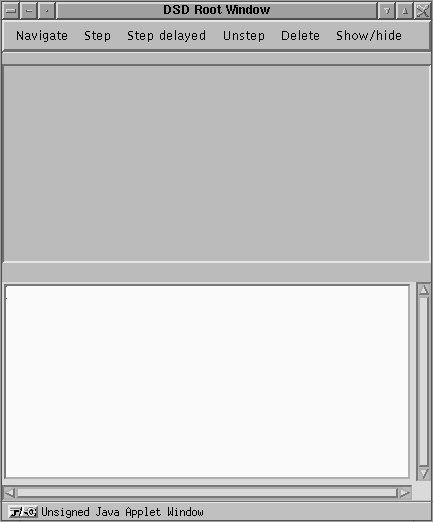
\includegraphics[scale=0.5]{FIGURES/dsdmain.png}
\caption{The main window of \dsd.}%
\end{center}
\end{figure}

This window consists of a menu bar at the top and two display areas.
Initially, both display areas are empty and the single item selectable
from the menu bar is {\tt Get~List} from menu {\tt Navigate}.

The lower display area of the root window is the so-called
{\em alert area}, where the applet displays messages addressed to the user.
Some of those messages originate in \dsd\ itself (they may---but don't
have to---refer to errors or problems encountered by the applet);
some others may be
notes (e.g., sent by {\tt displayNote}---\sect{rm_ex_in}) or error
diagnostics arriving from the \smurph\ program.

The upper display area (the {\em selection area\/}) is used to present
the list of objects that the user can select from at the moment.

The only sensible thing that can be done at the beginning, right after the
root window has been brought up, is to select {\tt Get~List} from the
{\tt Navigate} menu.
This will ask \dsd\ to try to connect to the monitor and acquire information
about all \smurph\ programs currently running.
This information will be displayed in a list (one program per line) in
the selection area.
If no \smurph\ programs are running at the moment, the message
``{\tt Nothing there}'' will appear in the alert area and nothing more
will happen.

If the list of programs displayed in the selection area is nonempty, the
user can select one program from the list and choose an item
from the {\tt Navigate} menu.
This menu now consists of the following two items:
\medskip

\begin{quote}
\noindent\hspace{-0.35in}{\bf {\tt Connect}}\\ \hspace{0in}
By hitting this item, the user asks \dsd\ to establish a display session
with the indicated program.
\end{quote}

\begin{quote}
\noindent\hspace{-0.35in}{\bf {\tt Status}}\\ \hspace{0in}
By hitting this item, the user asks \dsd\ to display short status
information about the indicated program.
\end{quote}\medskip

In the latter case, the applet will poll the indicated program
(using the monitor to mediate this communication) for its status.
In response, the program will send the following information that will appear
in the alert area of the root window:

\begin{itemize}
\item
the number of messages received so far by the standard {\tt Client}
(\sect{rm_po_wr_rp})
\item
the amount of virtual time (in {\em ITU\/}s)
elapsed since the program was started
\item
the amount of CPU time (in seconds) used by the program
\end{itemize}

If the user selects {\tt Connect} from the {\tt Navigate} menu,
the applet will try to set up a {\em display session\/}
with the selected \smurph\ program.

During a display session,
\dsd\ presents in the selection area a list
of objects whose dynamic exposures can be requested at the moment.
The list starts up with an initial selection of objects
sent by the \smurph\ program, and the
{\tt Navigate} menu provides a collection of
operations for navigating through these objects and requesting their
exposures (\sect{rm_ex}).
Depending on the current configuration of those exposures,
other menus from the menu bar may also become useful.

Each object exposure requested by \dsd\ appears in a separate window.
As explained in \sect{rm_ex_gc}, such an exposure corresponds to
a triplet: $<$object, display mode, station$>$.
The raw exposure information sent by the \smurph\ program is organized
by \dsd\ into a window based on the {\em window template}.

\subsection{Window templates}
\label{rm_ds_tp}

The material in this section may be useful for the user who would like to
create non-standard windows and/or define non-standard exposable types
(\sect{rm_ex_mo}).
It also helps to understand how the information
sent by the \smurph\ program to the \dsd\ applet is turned into windows.

The layout of a window is determined by the {\em window template}, which is
a textual pattern supplied in a {\em template file}.
A standard template file (providing templates
for all standard exposable objects of \smurph) is provided with the
monitor (\sect{rm_ds_mo}).
The monitor reads this file upon startup (\sect{rm_un_in}), and associates
standard templates with all object selections sent by a \smurph\ program
to the \dsd\ applet.
A \smurph\ program itself may use a private template file (\sect{rm_un_ru}),
which provides templates for its non-standard exposable objects and/or
overrides (some of) the standard templates.

A template file consists of template definitions; each template describing
one window layout associated with a combination of the object type,
the display mode, and a designator that determines whether the window
should be station-relative.

\subsubsection{Template identifiers}
\label{rm_ds_tp_ti}

The definition of a template starts with its identifier, which consists of
up to three parts.
Whenever the user requests a specific exposure,
\dsd\ searches the list of templates associated with the currently
selectable objects, matching their identifiers to the parameters of the
requested exposure.
These parameters specify the object, the display mode, and (optionally)
the station to which the exposure should be related.
Not surprisingly, the general format of a template identifier captures
the three parameters:

{\tt\begin{tabbing}
12345678\=1234\=1234\=1234\=1234\=1234\=1234\=1234\=1234\kill
\> {\em name\/} {\em mode\/} {\em sflag}
\end{tabbing}}

The first (mandatory) part of the template identifier should be a type name
or a nickname.
The template will be used to display windows associated
with objects of the given type, or objects whose nickname
(\sect{rm_st_on}) matches the given name.

The second argument specifies the display mode of the template.
If this argument is missing, the default mode 0 is assumed.

The last argument, if present, tells whether the window can be made
station-relative.
If this argument is absent, the window is global, i.e.,
the template cannot be used to display a station-relative version of the
window.
An asterisk in this place defines a station-relative window template.
Such a template can only be used, if the exposure request specifies a station
(any station) to which the window is to be related.
Two asterisks mean that the window represented by the template can
(but does not have to) be station-relative.
We say that such a template is ``flexible.''

When the user requests a new exposure
(identifying a selectable object---\sect{rm_ds_om_na}),
\dsd\ presents a menu listing all templates that match the object to be
exposed.
This menu consists of the following templates (appearing in this order):
\begin{itemize}
\item
templates whose {\em name\/} matches the nickname of the object
\item
templates whose {\em name\/} matches the type name of the object
\item
templates whose {\em name\/} matches the base type name of the object
(\sect{rm_st_on})
\end{itemize}

Within each class of templates, the ones defined privately by the
\smurph\ program 
take precedence over the standard ones (known by the monitor).

\subsubsection{Template structure}
\label{rm_ds_tp_ts}

The best way to describe how templates are defined is to look at a
specific example.
The following template resembles the standard template describing the layout of
the mode 0 {\tt Timer} window (see \sect{rm_ex_se_ti}):

{\small
\begin{verbatim}
Timer 0
"Wait requests (absolute)"
// Displays Timer wait requests coming from all stations
B0123456789012345678901234567890123456789012345678901234567890123456789012345+B
|~~~~~~~~Time~~~St~~~~Process/Idn~~~~~TState~~~~~~~~AI/Idn~~~~~Event~~~~~State| r
|%%%%%%%%%%%%& %%% %%%%%%%%%%/&&& %%%%%%%%%% %%%%%%%%%/&&& %%%%%%%%% %%%%%%%%%|
*                                                                             |
*                                                                             | 
*8                                                                            |+
**                                                                            |
E01234567890123456789012345678901234567890123456789012345678901234567890123456E
\end{verbatim}}

The second line of a template definition must be a quoted string describing
briefly the window's purpose.
This description will identify the template on the menu used to 
select the exposure mode.
The description string must not contain newline characters.

Any text following the closing quote of the
description string and preceding the first
line starting with `{\tt B}' or `{\tt b}' is
assumed to be a comment and is ignored.
Similarly, all empty lines, i.e.,
those containing nothing except possible blanks and/or {\tt tab} characters
are always skipped.

The next relevant
line of the template,
starting with the letter `{\tt B}', begins the description of the window layout.
The first and the last non-blank characters from this line are removed and the
length of whatever remains determines the width of the window.
All characters other than `{\tt +}'
are ignored: they are just counted to the window width.
A `{\tt +}' character is also counted, but it has a
special meaning: if present, it describes the initial width of the window
(the column tagged with `{\tt +}' is included).
Only one `{\tt +} may appear in the width line.
In the above example, the `{\tt +}' tag is superfluous: by default, the
initial width is equal to the full width.

The line starting with `{\tt B}' does not belong to the window frame and
it does not count to the window height.
Similarly, the closing line of the template (the one starting with `{\tt E}')
is not considered part of the window frame.
In fact, only the first character (the letter `{\tt E}') from the closing
line is relevant and the rest of that line is ignored.

\medskip

\noindent
{\bf Note:} `{\tt b}' and `{\tt e}' can be used instead of `{\tt B}' and
`{\tt E}', respectively.

\medskip

All nonempty lines, not beginning with `{\tt X}' or `{\tt x}' (see below),
occurring between the
starting and closing lines, describe the window contents.
Each such a line should begin with `{\tt |}' or `{\tt *}'.
A line beginning with `{\tt |}' is a {\em format\/} line: it gives the
layout of the corresponding window line.
A layout line terminates with a matching vertical bar.
The two bars do not count to the layout: they are just delimiters.
The terminating bar can be followed by additional information, which does
not belong directly to the layout, but may associate certain attributes
with the items defined within the line.

\subsubsection{Special characters}
\label{rm_ds_tp_sc}

Within the layout portion of a template line, some characters have special
meaning.
All non-special characters stand for themselves, i.e.,
they will be displayed directly on the positions they occupy within the
template.
Below we list the special characters and describe their meaning.

\medskip

\begin{quote}
\noindent\hspace{-0.35in}{\bf {\tt \char126}}\\ \hspace{0in}
This character stands for a virtual blank.
It will be displayed as a blank in the window.
Regular blanks are also displayed as blanks; however, two items separated
by a sequence of regular blanks are considered separate, in the sense that
each of them can have an individually definable set of attributes
(\sect{rm_ds_tp_at}).
\end{quote}

\begin{quote}
\noindent\hspace{-0.35in}{\bf {\tt \%}}\\ \hspace{0in}
A sequence of `{\tt \%}'s reserves space for one right-justified
data item sent by the {\smurph} program to be displayed in the window.
\end{quote}

\begin{quote}
\noindent\hspace{-0.35in}{\bf {\tt \&}}\\ \hspace{0in}
A sequence of `{\tt \&}'s reserves space for one left-justified
data item sent by the {\smurph} program
to be displayed in the window.
\end{quote}

\begin{quote}
\noindent\hspace{-0.35in}{\bf {\tt \char64}}\\ \hspace{0in}
This character is used to define a {\em region\/}, i.e., a semi-graphic
subwindow (sections \ref{rm_ex_pr}, \ref{rm_ds_tp_re}).
\end{quote}\medskip

Non-blank fields separated by a sequence of `{\tt \char126}'s
appear as different items, but
they are viewed as a single item from the viewpoint of their attributes.
Moreover, the separating sequence of virtual blanks receives the same
attributes as the fields it separates.
For example, the header line of the {\tt Timer} template contains a number
of items separated by virtual blanks.
The letter {\tt r} occurring after the terminating bar of the header
line says that the first item of this line is to be displayed in
{\em reverse video}.
However, from the viewpoint of this attribute, all the items of the header
line are viewed as a single item.
Therefore, the entire header line will be displayed in reverse.

A sequence of `{\tt \%}'s reserves an area to contain a
single data item sent to \dsd\ by the \smurph\ program as part of the
information representing the object's exposure (\sect{rm_ex_pr}).
The type of this item is irrelevant from the viewpoint of the
template declaration and will be determined upon arrival.
The program will attempt to contain the item within its field.
The item will be truncated, if it does not fit there, and right-justified,
if some space is left.
The only difference between `{\tt \&}' and `{\tt \%}' is that an item
displayed in a field described by a sequence of `{\tt \&}'s is left-justified.

Data items arriving from the \smurph\ program are assigned to their fields in
the order in which they arrive.
The order of fields is from left to right within a line and then, when the
line is filled, \dsd\ switches to the next line.
Superfluous data items are ignored.

\subsubsection{Exception lines}
\label{rm_ds_tp_ex}

A special character can be {\em escaped}, i.e., turned into a non-special
one in a way that does not affect the visible length of the layout line.
Namely, a layout line can be preceded by a line starting with the letter
`{\tt X}' or `{\tt x}', for {\em exceptions}.
A position marked in the exceptions line by `{\tt |}' indicates that a special
character occurring on that position in the next layout line is to be
treated as a regular character.

Sometimes two fields that are supposed to contain two different data items
arriving from the protocol program must be adjacent.
A column marked with `{\tt +}' in an exception line indicates the forced
end of a field occurring in the next layout line.
Any field crossing the position pointed to by the `{\tt +}' will be
split into two separate fields; the second field starting at the position
following the position of the `{\tt +}'.

A single layout line can be preceded by a number of exception lines, the
multiple exception lines being cumulative.

\subsubsection{Replication of layout lines}
\label{rm_ds_tp_rp}

Sometimes the same layout line has to be replicated a number of times.
In some cases this number is quite arbitrary.
Such a situation occurs with the {\tt Timer} window, which is actually a
table consisting of rows with exactly the same format (the header line
excepted).

A line starting with an asterisk stands for a
replication of the last regular layout line.
The asterisk can be followed by a positive integer number that says how
many replications are needed.
If the number is missing, 1 is assumed.
Double asterisk means that the number of replications is undefined:
the program is free to assume any nonnegative number.

A replication line need not contain any characters other than the asterisk
possibly followed by a number, or two asterisks.
However, if such a line is to contain an initial height indicator
(see below), it should be closed by the vertical bar, as the height
indicator can only appear after the bar.

\subsubsection{Window height}
\label{rm_ds_tp_wh}

The window height is determined by the number of the proper layout lines
(excluding the {\tt B}-line, the {\tt E}-line, empty lines, and exception
lines).
A layout line whose ``contents'' part terminates with a vertical bar can
include `{\tt +}'---the initial height indicator,
which should immediately follow the terminating bar.
If the height indicator
does not occur, the initial number of rows to be displayed in the window
is equal to the number of the proper layout lines of the template.

A height indicator occurring at a replication line with replication count
bigger than 1 is associated with the last line of this count.
A height indicator appearing at a `{\tt **}'-line or past this line is ignored.

If the window height is undefined
and no default height indicator occurs within the defined part,
the initial height of the window is determined by the number of proper
layout lines preceding the first replication line with undefined count.

\subsubsection{Regions}
\label{rm_ds_tp_re}

A region is a rectangular fragment of a window used to display graphic
information.
For an example of a region, let us look at the following template describing
a window for displaying the contents of a random variable:

{\small
\begin{verbatim}
                    RVariable 0
                    "Full contents"
                    B------------------------B
                    |@                      @|
                    |                        |
                    |                        |
                    |                        |
                    |                        |
                    |                        |
                    |                        |
                    |                        |
                    |                        |
                    |                        |
                    |@                      @|
                    |------------------------| r
                    |Count:  %%%%%%%%%%%%%%%%| h n
                    |Min:    %%%%%%%%%%%%%%%%| h n
                    |Max:    %%%%%%%%%%%%%%%%| h n
                    |Mean:   %%%%%%%%%%%%%%%%| h n
                    |StDev:  %%%%%%%%%%%%%%%%|+ h n
                    X    |                   X
                    |CI95%:  %%%%%%%%%%%%%%%%| n
                    |        %%%%%%%%%%%%%%%%| n
                    **                       |
                    E------------------------E
\end{verbatim}}

The template defines one region delimited by the four `{\tt \char64}' characters
that mark the region's corners.
The rows and columns containing these characters belong to the region.
Except for the delimiting characters, the rest of the rectangle representing
the region is ignored, i.e.,
any characters appearing there are treated as a comment.

A single template may define a number of regions.
Regions must not overlap and they must be perfectly rectangular.
The ordering of regions among themselves and other fields (important for
the correct interpretation of the data items arriving from \smurph) is
determined by the positions of their left top corners.

\subsubsection{Field attributes}
\label{rm_ds_tp_at}

A layout line terminated by `{\tt |}' can specify attributes to be associated
with its individual display items.
The optional specification of these attributes should follow the initial
height indicator, if one is associated with the line.

At most one attribute specification can be associated with a single item,
including regions.
Specifications for different items are separated by blanks.
The correspondence between specifications and items is determined by the
order of their occurrence from left to right.
Note that regions are represented for this purpose by their left top
corners.
Superfluous specifications are ignored.
Items without specifications are assigned default attributes.

The following attributes are defined:

\bigskip

\noindent
{\tt n~} normal display (the default)

\noindent
{\tt r~} reverse video

\noindent
{\tt h~} highlighted display

\noindent
{\tt b~} blinking display

\bigskip

Four attributes are applicable to a region; their specification can be put
at the region's first line, according to the same rules as for regular items.
Note that parentheses must be used if more than one attribute specification is
given. 

\subsubsection*{Example}

\noindent
Below we give an example of a window template defining two regions.
{\small
\begin{verbatim}
    Mytype 0 **
    "Just an example"
    B                      |                             B
    !Station~%%%%~~~~~~~~~~~~~~~~~~~~####################| h
    |@                     @  Number~of~packets: %%%%%%%%| r n b
    !                         Number~of~bits:    %%%%%%%%| n b
    |                         Acknowledgments:   %%%%%%%%| n h
    |                         Retransmissions:   %%%%%%%%| n n
    |                         Errors:            %%%%%%%%| n b
    |                         Average~delay:     %%%%%%%%| n h
    |                         ===========================| r
    |@                     @  @                 @  Status| h r
    |=======Variance========                       A %%%%| r h n
    |Hits:      %%%%%%%%%%%%                       B %%%%| h n h n
    |Misses:    %%%%%%%%%%%%                       C %%%%| h n h n
    |Total:     %%%%%%%%%%%%                       D %%%%| h n h n
    |Successes: %%%%%%%%%%%%                       E %%%%| h n h n
    |Failures:  %%%%%%%%%%%%                       F %%%%| h n h n
    |Total:     %%%%%%%%%%%%  @                 @  G %%%%| h n h n
    |Fairness:  %%%%%%%%%%%%  =======Mean========  H %%%%| h n r h n
    |~~~~~~~~~~~~~~~~~~~~~~~~~~~~~~~~~~~~~~~~~~~~~~~~~~~~| r
    E                                                    E
\end{verbatim}}

Note that the first region (the upper left one) is going to be displayed
in reverse, whereas the second one will be highlighted.

\subsection{Requesting object exposures}
\label{rm_ds_om}

As soon as a display session has been established, the \smurph\ program sends
to \dsd\ an initial list of exposable objects.
These objects are elements of the tree of all exposable objects currently
defined within the \smurph\ program.
The user can browse through that tree using the {\tt Navigate} menu
from the root window.

\subsubsection{The hierarchy of exposable objects}
\label{rm_ds_om_oh}

All exposable objects known to the \smurph\ program are logically organized
into a tree reflecting their {\em ownership\/} relation.
The root of this tree is the {\tt System} station (\sect{rm_to_st_cs})
which is assumed to own (directly or indirectly) all exposable objects.
The ownership relation is illustrated in
figure~7.
The ordering of subnodes reflects the order in which the objects represented
by the subnodes appear in the selection area of the root window
(\sect{rm_ds_li}).

%%% hoo.gif
\begin{figure}
\begin{center}
\ \resizebox{90mm}{!}{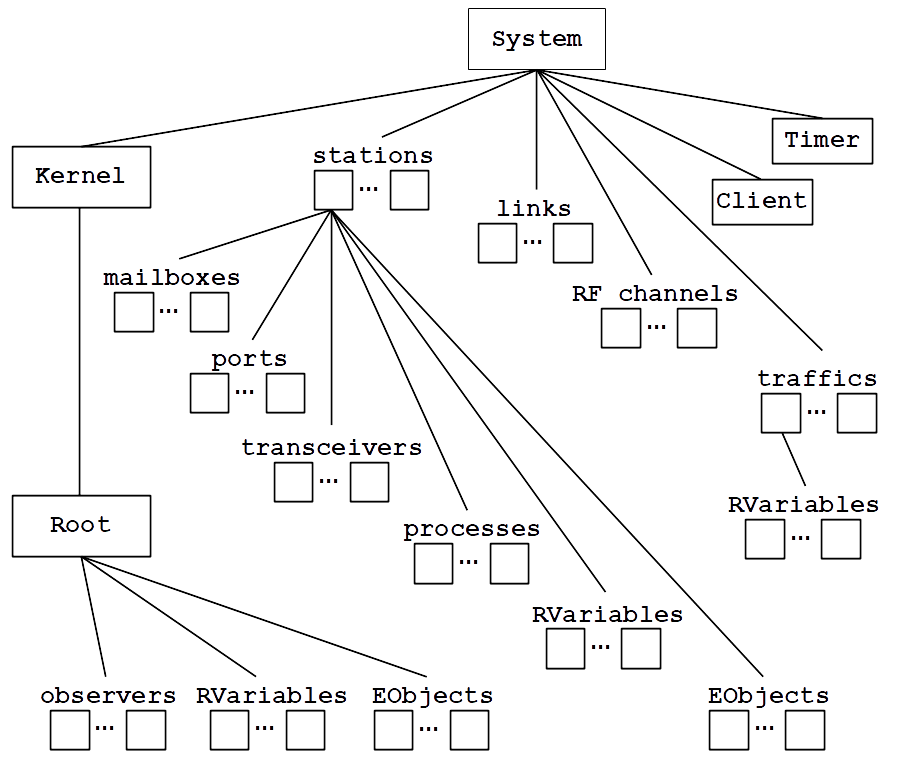
\includegraphics{FIGURES/hoo.png}}
\caption{The ownership hierarchy of exposable objects.}%
\end{center}
\end{figure}

The first object owned by {\tt System} is {\tt Kernel}---the root
of the process hierarchy (\sect{rm_pr_or}).
Note that the father-child hierarchy of processes
need not coincide with the ownership tree structure.
The {\tt System} station also owns all regular stations created by the 
protocol program.
These stations constitute a flat layer: they are all direct descendants
of {\tt System}.
Similarly, all links, radio channels,
traffic patterns, {\tt Client}, and {\tt Timer}
also belong to the {\tt System} station.

A regular station owns its mailboxes, ports and transceivers.
It also owns all regular processes, {\tt RVariables}, and {\tt EObjects}
that were created by {\tt Root}
in the context of the station (\sect{rm_pr_ct}).
The rules for determining the ownership of such objects created
while the protocol is running are different (see below).

Each traffic pattern is the owner of its collection of random variables
used
to keep track of the standard performance measures (\sect{rm_pm_cl_cv}).

The {\tt Kernel} process owns all system processes as well as 
the user-defined {\tt Root} process responsible
for initialization (\sect{rm_pr_or}).
The system processes are invisible to the user,
unless the \smurph\ program has been
called with the `{\tt -s}' option (sections \ref{rm_ex_se_ei}, \ref{rm_un_ru}).

The {\tt Root} process is the owner of all observers (\sect{rm_ob_ob}).
It also owns all
{\tt RVariables} and {\tt EObjects} that were created by
{\tt Root}, but outside the context of any regular station.

There are three categories of exposable objects that can be created (and
possibly destroyed) dynamically
by the protocol program after the initialization phase, namely:
processes, random variables, and {\tt EObjects}.
Any such object is owned by the process directly responsible for creating
it.
Thus, the ownership structure of processes created by other protocol
processes coincides with the father-child relationship.

\subsubsection{Navigating through the ownership tree}
\label{rm_ds_om_na}

At any moment during a display session, the list of objects presented in
the selection area consists of all the descendants of exactly
one object in the ownership tree.
The top item on that list (displayed in a different color) is the owner
itself.
Initially, immediately after the display session is established,
the \smurph\ program sends to \dsd\ the list of descendants of the
{\tt System} station, i.e., the root layer of the tree.

Each line in the selection area corresponds to one object and includes
up to three names of the object (if they all exist and are different):
the standard name, the base name, and the nickname.
An object can be selected by clicking on its line and unselected by clicking
once again.
The following three items from the {\tt Navigate} menu refer to the
objects listed in the selection area:
\medskip

\begin{quote}
\noindent\hspace{-0.35in}{\bf {\tt Descend}}\\ \hspace{0in}
\dsd\ asks the \smurph\ program to send the list of descendants of the
selected object.
This way the user descends one level down in the ownership tree.
\end{quote}

\begin{quote}
\noindent\hspace{-0.35in}{\bf {\tt Ascend}}\\ \hspace{0in}
\dsd\ asks the program to send the list of descendants of the object whose
immediate descendant is the owner of the currently presented list of objects.
This way the user ascends one level up in the ownership tree.
Of course, it is impossible to ascend above the {\tt System} station.
\end{quote}

\begin{quote}
\noindent\hspace{-0.35in}{\bf {\tt Display}}\\ \hspace{0in}
\dsd\ opens a dialog to select the display mode and/or the station-relative
status of an exposure for the selected object.
\end{quote}
\medskip

Each list of objects arriving from the \smurph\ program in response to a
descend/ascend request is accompanied by a list of templates applicable to
those objects.
Those templates are selected by the \smurph\ program itself (if it uses a
private template file) and/or by the monitor (using the standard set of
templates).

In response to {\tt Display}, \dsd\ shows a dialog listing all the templates
applicable to the selected object.
For example,
figure~8
presents the display dialog for the {\tt Kernel}
process (the first child item on the initial selection list).

%%% dsddial.gif
\begin{figure}
\begin{center}
\ 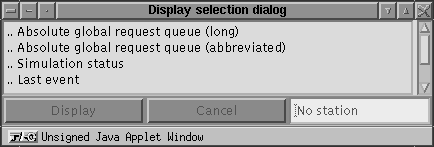
\includegraphics[scale=0.5]{FIGURES/dsddial.png}
\caption{A sample display dialog.}%
\end{center}
\end{figure}

The scrollable list includes all templates (their description
strings---\sect{rm_ds_tp_ts}) potentially applicable to the selected object.
Note that each template implicitly determines a display mode.
Thus, the only additional
element that must be specified to complete the exposure request is
the station {\tt Id}.
This item can be typed in the text area (the rightmost area
in the bottom panel).

The template description string starts with two characters that indicate the
station-relative status of the template.
Two periods mark an absolute template, i.e., one that cannot be related to
a station.
In such a case, the station field in the dialog is irrelevant and the template
itself fully describes the exposure.
For the remaining two cases (`{\tt .*}' meaning ``station-relative'' and
`{\tt **}' meaning ``flexible''---\sect{rm_ds_tp_ti}),
the field is meaningful.
If it contains a legal station number (it must for a station-relative
template), the exposure is station-relative; otherwise, it is absolute.

Having selected the template and (possibly) the station {\tt Id},
the user may click {\tt Display} to actually request the exposure.
In response to this action, \dsd\ will create a new window on the screen
(based on the template---\sect{rm_ds_tp}) and notify
the protocol program that a new exposure should be added to its internal
list of active exposures.
\dsd\ refuses to create a new exposure
if exactly the same exposure is already present.

\subsection{Exposure windows}
\label{rm_ds_wm}

Typically, an exposure window contains a number of static components
(extracted from the template---\sect{rm_ds_tp_ts}) and some
dynamic components that are
filled dynamically by the protocol program (\sect{rm_ex_in}).
Note that the the protocol program only sends the raw data---the layout of the
dynamic components within the window is determined by the template.

\subsubsection{Basic operations}
\label{rm_ds_wm_gc}

As soon as it is created, a new exposure appears in four menus selectable
from the root window: {\tt Step}, {\tt Step~delayed}, {\tt Delete},
and {\tt Show/hide}.
The exposure is identified in the menu by the name of the exposed
object,\footnote{This is the nickname, if one is defined, or
the standard name, otherwise.}
followed by the exposure mode in square brackets.
If the exposure is station-relative, this string is further followed by
the station {\tt Id} in parentheses.

By selecting the exposure from the {\tt Show/hide} menu, the user
toggles its ``visible'' status, i.e., the window becomes invisible if it
was visible and vice versa.
A window that becomes visible is automatically forced to the top.
An invisible exposure window remains active and it continues receiving
updates from the protocol program.

An exposure can be canceled by selecting it from the {\tt Delete} menu.
In response to this action, \dsd\ removes the exposure's window from the
screen and notifies the \smurph\ program to remove the exposures from its
internal list.

An exposure window can be naturally resized.
If the entire contents of the exposure cannot fit into whatever frame
is made available for the window,\footnote{This is rather typical for
windows with undefined height---\sect{rm_ds_tp_wh}.}
the visible area can be scrolled.
This is done by clicking and dragging in the visible area.

To reduce the amount of traffic between the protocol program and \dsd,
the protocol program maintains two counters for each active exposure.
One of them tells the number of the first visible item in the current
version of the exposure's window, the other specifies the number of the
first item that is not going to show up.
Whenever a window is resized or scrolled, \dsd\ sends to the protocol
program new values of the two counters.
As only those items that actually appear in the window are sent in
window updates,
the scrolled-in area of a window may initially appear blank.
It will become filled as soon as the protocol program learns about the
new parameters of the window and begins sending the missing items.

\subsubsection{Stepping}
\label{rm_ds_wm_sm}

A protocol program can be put into the so-called
{\em step mode\/} in which it stops on some (or all) events.
An explicit user action is then required to continue execution.

The step mode is always requested for a specific exposure window.
If a window is {\em stepped}, the \smurph\ program is halted whenever an event
occurs that is somehow ``related'' to the exposure.
At that moment,
the contents of the window reflect the program state {\bf after}
the event has been processed.

Multiple exposures can be stepped at the same time.
The occurrence of any event related to any of the stepped windows stops the
protocol program.

The following rules describe what we mean by an
``event related to the exposure'':
\begin{itemize}
\item
If the exposed object is a station, the related event is any
event waking any process owned by the station.
\item
If the object is a process, the related event is any event waking the process.
One exception is the {\tt Kernel} process.
It is assumed that all events are related to {\tt Kernel}; thus, by
stepping any {\tt Kernel} exposure you will effectively monitor all events.
\item
If the object is a random variable or an
exposable object of a user-defined type,
the related event is any event related to the object's owner (in the
sense of \sect{rm_ds_om_oh}).
\item
If the object is an observer, the related event is any
event that results in restarting the observer.
\item
If the object is an {\em AI\/} not mentioned above, the related event
is any waking event triggered by the {\em AI}.
\end{itemize}

To put an exposure window immediately
into the step mode the user should select it from the {\tt Step}
menu.\footnote{Key shortcuts are available---see~\sect{rm_ds_sh}.}
The frame of a stepped window changes its color from blue to red.

It is also possible to step an exposure at some later moment, by selecting
it from the {\tt Step~delayed} menu.
This may be useful for debugging: the user may decide to run the program
at the full speed until it has reached some interesting stage.
In response to {\tt Step~delayed}, \dsd\ presents a dialog shown
in
figure~9.

%%% dsdstep.gif
\begin{figure}[htbp]%
\begin{center}
\ 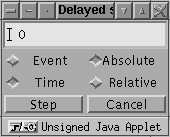
\includegraphics{FIGURES/dsdstep.png}
\caption{The step dialog.\label{fig.dsdstep}}%
\end{center}
\end{figure}%

The step dialog allows the user to select the virtual time when the
stepping should commence, or the number of events to be processed before
it happens.
This number can be either absolute or relative, i.e., represent an offset
with respect to the current time or event count.
Note that the first stepped event has to ``have something to do'' with the
stepped exposure, so it may occur later (but no earlier)
than the specified time.

The occurrence of a stepped event forces the protocol program to
immediately (regardless of the value of
{\tt DisplayInterval}---\sect{rm_ex_in}) send the update information for
all active exposures and halt.
The program will not resume its execution until the user selects
{\tt ADVANCE} from the {\tt Step} menu.
Then the program will continue until the next stepped event and halt again.
Each time this happens, the message {\tt STEP} is displayed in the
alert area of the root window (\sect{rm_ds_li}).

The user can cancel the stepping for one exposure---by selecting it from the
{\tt Unstep} menu, or globally for all stepped exposures---by selecting
{\tt ALL} from that menu.
If this is done when the program is halted, {\tt ADVANCE} is still required
to let it go.
Alternatively, the user may select {\tt ALL+GO} from the {\tt Unstep}
menu to cancel all stepping and resume the normal execution of the program.

\medskip
\noindent
{\bf Note:}
Stepping affects the real-time character of the \smurph\ program and is not
recommended for monitoring the behavior of a control
program driving real equipment.

\medskip
\noindent
{\bf Note:}
When the display session is requested by the \smurph\ program
(\sect{rm_ex_in}), also when the program is called with {\tt -d} 
(\sect{rm_un_ru}), the program appears halted at the very beginning of the
display session, although no exposure is formally being stepped.
{\tt ADVANCE} or {\tt ALL}({\tt +GO})---selected from the
{\tt Unstep}---menu can be used to resume the execution of such a program.

\subsubsection{Segment attributes}
\label{rm_ds_sa}

The attribute pattern of segments (\sect{rm_ex_pr}) is interpreted by
\dsd\ in the following way (bits are numbered from zero starting from the
less significant end):


\begin{quote}
\noindent\hspace{-0.35in}{\bf Bits 0--1}\\ \hspace{0in}
This field is interpreted as a number from 0 to 3 specifying the segment
type.
The following types are supported:
0--discrete points, 1--points connected with lines, 2--discrete stripes
extending to the bottom of the region area.
\end{quote}

\begin{quote}
\noindent\hspace{-0.35in}{\bf Bits 2--5}\\ \hspace{0in}
Thickness.
This field is ignored for type--1 segments (i.e., points connected with
lines).
Otherwise, it represents the thickness of points or stripes,
which, expressed in pixels, is equal to the numerical value of this field~+2.
\end{quote}

\begin{quote}
\noindent\hspace{-0.35in}{\bf Bits 6--13}\\ \hspace{0in}
Color.
The numerical value of this field is used as an index into the internal
color table of \dsd\ and determines the color of the segment.
\end{quote}

\subsection{Other commands}

In this section, we discuss briefly some other commands of \dsd\ that are
not directly related to exposure windows.

\subsection{Display interval}

As we mentioned in \sect{rm_ex_in}, a \smurph\ program engaged in a display
session with \dsd\ sends exposure updates at intervals determined by the
value of {\tt DisplayInterval}.
In the simulation (virtual) mode, this interval is expressed in events, and
in the real (and also visualization)
mode it is in milliseconds.
In \sect{rm_ds_wm_sm}, we noted one exception from this rule: when the program
is stepped, it sends an update as soon as it is halted, regardless of the
prescribed interval between regular updates.

The value of {\tt DisplayInterval} can be changed by selecting
{\tt Reset~Refresh~Interval} from the {\tt Navigate} menu.
In response to this selection, \dsd\ presents a simple dialog
shown in
figure~10.

%%% dsddin.gif
\begin{figure}[htbp]%
\begin{center}
\ 
\includegraphics{FIGURES/dsddin.png}
\caption{The display interval dialog.}%
\end{center}
\end{figure}%

The number entered in the text area represents the new requested value of the
display interval, which is either in events or in milliseconds, depending
on whether the program runs as a simulator, or executes in the real mode.
The display interval cannot be reset
in the visualization mode where it is coupled
to the resync grain (\sect{rm_pr_vi}).

\subsection{Disconnection and termination}

By selecting {\tt Disconnect} from the {\tt Navigate} menu, the user
terminates the display session.
\dsd\ notifies the \smurph\ program that it should not send any more
updates and it should not expect any more commands from \dsd.

All the windows of \dsd\ remain on the screen until either the root window
is canceled (by hitting the {\tt Stop} button on the applet's startup panel)
or a new selection is made from the {\tt Navigate} menu (which at this
stage can only be {\tt Get~List}---\sect{rm_ds_li}).

It is possible to terminate the \smurph\ program from \dsd---by selecting
{\tt Terminate} from the {\tt Navigate} menu (during a display
session).
As this action is potentially dangerous, {\tt Terminate} must be selected
twice in a row to be effective.

\subsection{Shortcuts}
\label{rm_ds_sh}

The following key strokes can be used as shortcuts for some \dsd\ actions
(normally selectable from menus).
They are only effective if hit while within an exposure window.

\noindent
{\tt s~} immediate step for this exposure ({\tt Step})

\noindent
{\tt S~} delayed step for this exposure ({\tt Step~delayed})

\noindent
{\tt u~} unstep this exposure ({\tt Unstep})

\noindent
{\tt U~} unstep this exposure and go

\noindent
{\tt g~} continue until next step ({\tt ADVANCE})

\medskip

The last key (``{\tt g}'') can be hit in any window, including the root window,
and its semantics is always the same: ``continue until the next stepped
event.''
Upper case ``{\tt G}'' and the space bar can be used instead of ``{\tt g}''
and their meaning is exactly the same.

%%%@@@-- unixw.tex
\section{\smurph\ under UNIX and Windows}
\label{rm_un}

This section contains information on using \smurph\ in the UNIX
environment and under CYGWIN on Windows 98, XP and Vista.

In principle, \smurph\ can be installed on any machine running
a BSD or POSIX-compatible UNIX system, equipped with the GNU C++ compiler.
The package has been also successfully installed on many machines
and UNIX systems using several versions of C++ compilers.
Under Windows, \smurph\ runs within the Cygwin environment available
from {http://www.cygwin.com/}.

To take advantage of \dsd, a Java environment is needed.
This environment (and \dsd) may
be installed on the machine (or machines) on which
\smurph\ experiments are to be run.
Alternatively, \dsd\ may be invoked from another machine and communicate
with the experiment (or experiments) via the network.

%%%CHKP One hardware-dependent feature of \smurph\ is {\em checkpointing}
%%%CHKP (see \sect{rm_un_ch}): the code implementing it must be written
%%%CHKP separately for each machine type.
%%%CHKP This feature is useful for simulation but irrelevant for control
%%%CHKP applications of \smurph.

\subsection{Installation}
\label{rm_un_in}

The package comes as a collection of files organized into the directory
structure presented in
figure~11.
The root directory of the package contains the following items:

\medskip

\begin{quote}
\noindent\hspace{-0.35in}{\bf {\tt MANUAL}}\\ \hspace{0in}
This directory contains the PDF version of this manual.
\end{quote}

\begin{quote}
\noindent\hspace{-0.35in}{\bf {\tt SOURCES}}\\ \hspace{0in}
This directory contains the source code of the package.
\end{quote}

\begin{quote}
\noindent\hspace{-0.35in}{\bf {\tt Examples}}\\ \hspace{0in}
This directory includes a number of sample protocols programmed in
\smurph.
\end{quote}

\begin{quote}
\noindent\hspace{-0.35in}{\bf {\tt README.txt}}\\ \hspace{0in}
This file contains the copyright notice and the log of changes
introduced to the package since version 0.9 until the end of August 2006.
\end{quote}

\begin{quote}
\noindent\hspace{-0.35in}{\bf {\tt RTAGS\_PG}}\\ \hspace{0in}
Log of changes starting at March 3, 2006 until present.
\end{quote}

\begin{quote}
\noindent\hspace{-0.35in}{\bf {\tt INSTALL.txt}}\\ \hspace{0in}
Installation instructions.
\end{quote}

\begin{quote}
\noindent\hspace{-0.35in}{\bf {\tt scopy}}\\ \hspace{0in}
This is a shell script used to create a copy of the package by
linking some files to the original (see below).
\end{quote}\medskip

%% sds.gif
\begin{figure}
\begin{center}
\ 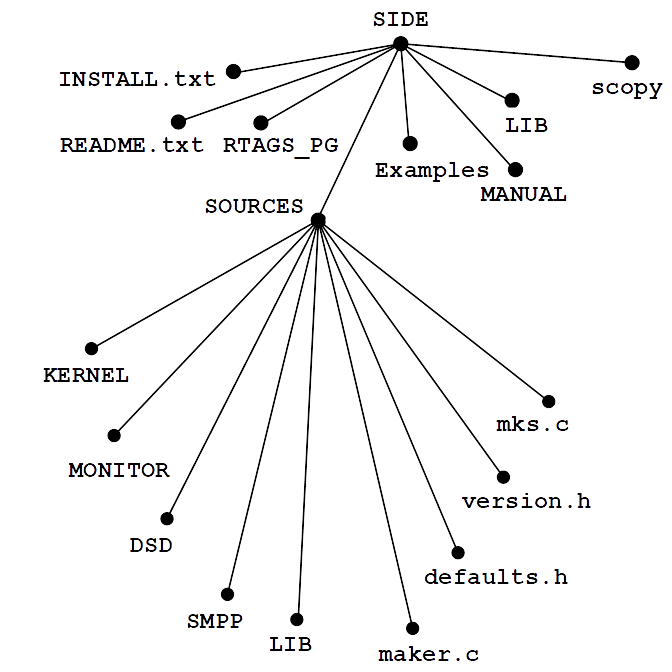
\includegraphics[scale=0.5]{FIGURES/sds.png}
\caption{The structure of \smurph\ directories.}%
\end{center}%
\end{figure}%

The vital parts of the package are contained in directory {\tt SOURCES}
which consists of the following entries:

\medskip

\begin{quote}
\noindent\hspace{-0.35in}{\bf {\tt KERNEL}}\\ \hspace{0in}
This is a directory that contains the source code of the \smurph\ kernel.
These files are used to create \smurph\ libraries that are configured with
the user-supplied protocol files into stand-alone \smurph\ programs.
\end{quote}

\begin{quote}
\noindent\hspace{-0.35in}{\bf {\tt MONITOR}}\\ \hspace{0in}
This directory contains the source files of the monitor used to keep track
of \smurph\ programs in execution
and to connect them to \dsd\ (\sect{rm_ds_mo}).
\end{quote}

\begin{quote}
\noindent\hspace{-0.35in}{\bf {\tt DSD}}\\ \hspace{0in}
This directory contains the source and Java-machine
code of the display applet \dsd\ (\sect{rm_ds}).
\end{quote}

\begin{quote}
\noindent\hspace{-0.35in}{\bf {\tt SMPP}}\\ \hspace{0in}
This directory contains the source code of the preprocessor 
(\smurph\ compiler) which is run before the C++ compiler
to turn \smurph\ constructs into C++ code.
\end{quote}

\begin{quote}
\noindent\hspace{-0.35in}{\bf {\tt LIB}}\\ \hspace{0in}
This directory contains the source code of the \smurph\ 
i/o and XML library.
\end{quote}

\begin{quote}
\noindent\hspace{-0.35in}{\bf {\tt maker.c}}\\ \hspace{0in}
This is the source code of {\tt maker}---the
program used to configure the package (see below).
\end{quote}

\begin{quote}
\noindent\hspace{-0.35in}{\bf {\tt defaults.h}}\\ \hspace{0in}
This file contains definitions of default values to be used by the
configuration program {\tt maker}.
\end{quote}

\begin{quote}
\noindent\hspace{-0.35in}{\bf {\tt version.h}}\\ \hspace{0in}
This file contains the version number of the package and the code for
recognizing the C++ compiler version.
\end{quote}

\begin{quote}
\noindent\hspace{-0.35in}{\bf {\tt mks.c}}\\ \hspace{0in}
This is the source code of {\tt mks}---the driver for the \smurph\ compiler.
\end{quote}\medskip

Another directory named {\tt LIB} appears at the root level of the
directory tree.
It is initially empty, and its purpose is to contain binary versions
of the kernel (\sect{rm_un_cr}).

Before the package is installed, the user must make sure that the target
machine is equipped with the tools needed to compile the package.
For the UNIX environment, this is usually the case.

The version of \dsd\ included with the package assumes JDK (Java Development
Kit) which can be downloaded from
{http://www.java.com/}.
Note that the specification and execution system of \smurph\ can be used
without \dsd.

To install the package, the user should unpack the \smurph\ directory tree
anywhere in his directory, e.g., by executing:
\begin{verbatim}
        zcat sidexxx.tar.gz | tar -xvf -
\end{verbatim}
\noindent
where ``{\tt xxx}'' stands for the current version of the package.

A single copy of the package can be shared by a number of users.
In such a case, instead of copying all files, the user should perform the
following two steps:

\begin{enumerate}
\item
create the \smurphtt\ directory and move there
\item
execute the {\tt scopy} script by entering
{\tt\begin{tabbing}
12345678\=1234\=1234\=1234\=1234\=1234\=1234\=1234\=1234\kill
\> {\em prfx\/}{\tt /scopy}
\end{tabbing}}
where {\em prfx\/} is the path to the {\tt scopy} script in the original
\smurphtt\ directory
\end{enumerate}

In consequence of the above operations, a copy of the \smurphtt\ directory
tree will be built, but only those files that may change in different
instances of the package will be physically duplicated.
All other files, notably all source files of the \smurph\ kernel,
monitor, and \dsd, will be represented by links to the originals.

Then the user should move to the {\tt SOURCES} subdirectory
and compile the {\tt maker} program by executing
\begin{verbatim}
        g++ -o maker maker.cc
\end{verbatim}

Having created {\tt maker}, the user is ready to configure \smurph.
This is done by executing
\begin{verbatim}
        maker
\end{verbatim}
and responding to a few questions asked by the program.
In most cases, the default answers (indicated by {\tt maker}) make sense
and are recommended.
The program asks about the following things:

\begin{itemize}
\item
The name of the Java compiler.
This information is only relevant and needed if the user
wishes to recompile the \dsd\ applet.
Normally, the applet need not be recompiled because the precompiled Java code
is platform-independent.
\item
The path to the {\tt SOURCES} directory, i.e., to the directory containing
the source files of the package.
The default (which practically never should be changed)
is the current directory.
\item
The path to the directory where binary libraries of the kernel modules
will be kept.
The default path is ``{\tt ../LIB}'', i.e., the libraries will be kept in
subdirectory {\tt LIB} in the root directory of the package.
This default practically never needs to be changed.
\item
The maximum number of versions of the binary library to be kept in the
library directory (see \sect{rm_un_cr}).
The default number is 25.
\item
The name of the directory containing {\tt include} files for protocol programs.
It is possible to have several simultaneous versions of such {\tt include}
libraries, which will be searched in the order of their specification.
By default, the standard library in {\tt Examples/IncLib} is made available.
It is needed by the example protocol programs in {\tt Examples}, but it also
contains many handy pieces that may be of general value, so it always makes
sense to have it on the list.
When you hit Enter (empty line) in response to this prompt, the standard
{\tt include} library will be the only library used.
You can also enter paths to your personal libraries, one path per line, and
then they will add to the list.
You can eliminate the standard library (at any moment) by entering a line
containing `{\tt -}' (minus) as the only character.
An empty line always terminates the list.
\item
The name of the directory containing the (optional)
library for XML data files
{\em included\/} (see \sect{rm_au_io_xm}) from XML data sets.
Multiple such directories can be specified: they will be
scanned in the order of their definition.
An empty line terminates the sequece of data include directories.
\item
The Internet
name of the host running the \smurph\ monitor (\sect{rm_ds_mo}).
Note that the monitor is needed to provide an interface between programs
in \smurph\ and the \dsd\ applet.
Even if all three parties are to be run on the same machine, the host name
of that machine must be specified here.
By default, there is no monitor host, which means that the \dsd\ applet
will never be used.
Enter {\tt localhost} to be able to
run all three components on the same local machine.
\item
The number of the monitor socket port.
This should be an unused port number for implementing an {\tt AF\_INET}
socket available to non-privileged users.
The default number is 4442.
\item
The name of the \smurph\ compiler.
The default name is ``{\tt mks}'' and there is little sense in changing it.
\item
The directory where {\tt mks} is to be put.
The default is ``{\tt {\char126}/bin}'' where ``{\tt \char126}'' stands for the
user's home directory.
This directory should be included in the {\tt PATH}.
\item
Whether the monitor is to be created.
If the answer is ``{\tt yes}'' (which is the default), {\tt maker} will create
the binary version of the monitor and put it into directory {\tt MONITOR}.
\end{itemize}

When {\tt maker} is done, it updates the contents of file
{\tt version.h} in directory {\tt SOURCES} to reflect some of the user's
selections.

The library directory ({\tt LIB}) will be used by
{\tt mks} to keep binary versions of the kernel files (see \sect{rm_un_cr}).
This directory is initially empty.
If it already exists and contains something, {\tt maker} will erase all its
contents.
The maximum number of versions tells how many different versions of the binary
files (corresponding to different configurations of {\tt mks} parameters)
can be kept simultaneously in the library directory.
The bigger this number, the less time it takes on the average to generate a
new simulation instance, at the expense of disk space (\sect{rm_un_cr}).
On Linux, one library version takes about 4MB of disk space.

The monitor should be created on one designated host.
Preferably, it should be a workstation owned by the user.
The executable version of the monitor is put into file {\tt monitor}
in directory {\tt MONITOR}.
The user should move there and run the monitor in the background by
executing
\begin{verbatim}
        monitor standard.t &
\end{verbatim}
The parameter identifies the standard template file, which is supplied
in the monitor's directory (see sections \ref{rm_ds_mo} and \ref{rm_ds_tp}).

The monitor should be running all the time.
It uses very little resources and its impact on the workstation's
performance is completely negligible.

There is a small
chance that the monitor will exit immediately with the following diagnosis:
\begin{verbatim}
        port probably taken, rebuild with another socket port
\end{verbatim}
which means that the monitor has failed to open an {\tt AF\_INET} domain socket.
Such a problem may occur if the port number assigned by {\tt maker} to
the socket is in use.
The user should execute {\tt maker} once again selecting another port number.
Typically, legal values are between 2000 and 32000.
Note that selecting a new port generally involves a recompilation of
the package.

The package includes two versions of the monitor: one implemented as a
typical UNIX daemon that spawns a separate process for each non-trivial
service, and the other implemented as a single process emulating multiple
service threads.
By default, the first version is used under UNIX and the second under
CYGWIN.

With the operation of starting the monitor, the installation of the package
is complete.

The \dsd\ applet can be invoked from an applet viewer or from a web browser.
File {\tt index.htm}
in directory {\tt DSD} provides an {\tt html} anchor to the applet.
Note that most browsers will not let the applet connect to the monitor
unless the web server delivering the applet runs on the same host as the
monitor.
Therefore, it may make sense to install a web server
(e.g.,
Apache---{http://www.apache.org/})
on the monitor host.
Alternatively, the monitor can be run on a host on which a web server has been
already installed.

It may be better and more convenient to run \dsd\ from {\tt appletviewer}
provided with the JDK distribution.
To do it, the user should move to the applet directory ({\tt SOURCES/DSD})
and execute
\begin{verbatim}
        appletviewer index.htm
\end{verbatim}

To let the applet freely connect to the monitor (even if both parties
happen to run
on the same host, the appletviewer may think that the session involves
communication across the network), the user should select {\bf unrestricted}
access to the network and classes from the ``properties'' dialog of the
appletviewer's menu.

Another minor problem related to the \dsd\ applet is the different look
of windows on different Java platforms.
This problem mostly concerns exposure windows and is not very serious,
as the window contents can be scrolled manually (\sect{rm_ds_wm_gc}) if
they appear misaligned.
Ultimately,
the user can edit file {\tt DSD.java} in {\tt SOURCES/DSD} and modify the
constants {\tt TOPMARGIN} and {\tt BOTTOMMARGIN} declared at the
beginning of class {\tt DisplayWindow}---to adjust the initial location
of the window contents permanently for the preferred platform.

\subsection{Creating executable programs in \smurph}
\label{rm_un_cr}

A user-supplied protocol program in \smurph\ must
be compiled and linked with the kernel
files to create a stand-alone executable file.

The protocol program may consist of a number of C++ files, the name of
a file ending with the suffix ``{\tt .cc}''.
All these files should be kept in one directory.
They may {\tt \#include} some user-created ``{\tt .h}'' files.
The \smurph\ preprocessor ({\tt smpp}) will automatically insert some standard
include files (from {\tt SOURCES/KERNEL}) in front of each protocol file.

To create an executable program for a given protocol source, the user
should move to the directory containing the protocol files and execute
{\tt mks} (we assume that the default name of the program has not been
changed at installation).
The program accepts the following arguments (in an arbitrary order):

\medskip

\begin{quote}
\noindent\hspace{-0.35in}{\bf {\tt -a}}\\ \hspace{0in}
All references to {\tt assert} are turned into empty statements
(see \sect{rm_au_eh}).
This may speed up the execution a little at the expense of some potential
errors passing undetected.
If this argument is not used, {\tt asserts} are active.
\end{quote}

\begin{quote}
\noindent\hspace{-0.35in}{\bf {\tt -b}}\\ \hspace{0in}
This argument must be followed by a single digit indicating the selected
precision of type {\tt BIG} (see \sect{rm_mp_vr}).
The number should be separated from `{\tt -b}' by a space.
The default precision of {\tt BIG} is 2.
\end{quote}

\begin{quote}
\noindent\hspace{-0.35in}{\bf {\tt -d}}\\ \hspace{0in}
If the argument is not followed by one the letters {\tt B}, {\tt L}, or
{\tt l} (separated from {\tt -d} by a space), then it says that
type {\tt DISTANCE} (\sect{rm_mp_ot}) will be defined as {\tt BIG}.
By default, if the argument is absent, type {\tt DISTANCE} is equivalent to
{\tt LONG}.
If {\tt -d} is followed by {\tt l}, then type {\tt DISTANCE} will be defined
as {\tt Long}.
{\tt B} following {\tt -d} is equivalent to {\tt -d} occurring alone
({\tt DISTANCE} defined as {\tt BIG}), and {\tt L} is
equivalent to no argument at all (the default case of type {\tt DISTANCE}
being defined as {\tt LONG}).
\end{quote}

\begin{quote}
\noindent\hspace{-0.35in}{\bf {\tt -f}}\\ \hspace{0in}
The C++ compiler will be called with the optimization option.
The default is ``no optimization.''
\end{quote}

\begin{quote}
\noindent\hspace{-0.35in}{\bf {\tt -g}}\\ \hspace{0in}
This argument indicates that a ``debug'' version of the program is to be
created.
The C++ compiler will be called with the debugging option;
simulator-level tracing (\sect{rm_ob_st}) will be enabled.

\noindent
An alternative variant of this option is {\tt -G}.
It is almost identical to {\tt -g}, but it additionally disables catching 
signals (like SIGSEGV) by \smurph\ and makes sure to trigger a hard error
(like SIGSEGV) when {\tt excptn} (\sect{rm_au_eh}) is called.
This makes it easier to catch and diagnose some errors (including violations
of internal assertions) in {\tt gdb}.
\end{quote}

\begin{quote}
\noindent\hspace{-0.35in}{\bf {\tt -i}}\\ \hspace{0in}
This argument determines the definition of type {\tt BITCOUNT}
(\sect{rm_mp_ot}) in the same way that argument {\tt -d} determines the
definition of type {\tt DISTANCE} (see above).
\end{quote}

\begin{quote}
\noindent\hspace{-0.35in}{\bf {\tt -m}}\\ \hspace{0in}
Error checking for operations on {\tt BIG} numbers, for
precision higher than 1, will be suppressed (see \sect{rm_mp_ao}).
Using this argument may slightly reduce the execution time at the price
of possibly missing some arithmetic errors.
\end{quote}

\begin{quote}
\noindent\hspace{-0.35in}{\bf {\tt -n}}\\ \hspace{0in}
Clock tolerance (\sect{rm_ti_to})
will be set to 0, irrespective of the requirements of the
protocol program.
This argument effectively removes all code for randomizing time delays and
makes all local clocks absolutely accurate.
\end{quote}

\begin{quote}
\noindent\hspace{-0.35in}{\bf {\tt -p}}\\ \hspace{0in}
This option enables the three-argument variants of wait requests.
A wait request may now specify an optional {\tt order} parameter that
assigns a priority to the wait request (sections \ref{rm_pr_ai},
\ref{rm_pr_po}).
\end{quote}

\begin{quote}
\noindent\hspace{-0.35in}{\bf {\tt -q}}\\ \hspace{0in}
This option enables the message queue size limit described in
\sect{rm_cl_mq}.
By default this feature is disabled.
\end{quote}

\begin{quote}
\noindent\hspace{-0.35in}{\bf {\tt -z}}\\ \hspace{0in}
This option enables ``faulty links'' described in \sect{rm_po_fl}.
By default ``faulty links'' are disabled.
\end{quote}

\begin{quote}
\noindent\hspace{-0.35in}{\bf {\tt -o}}\\ \hspace{0in}
This argument must be followed by a file name (separated from `{\tt -o}' by
a space).
The specified file will contain the executable \smurph\ program.
The default file name, assumed in the absence of `{\tt -o}',
is ``\smurphtts.''
\end{quote}

\begin{quote}
\noindent\hspace{-0.35in}{\bf {\tt -r}}\\ \hspace{0in}
This argument determines the definition of type {\tt RATE}
(\sect{rm_mp_ot}) in the same way that argument {\tt -d} determines the
definition of type {\tt DISTANCE} (see above).
\end{quote}

\begin{quote}
\noindent\hspace{-0.35in}{\bf {\tt -u}}\\ \hspace{0in}
The standard client is permanently disabled, i.e., no traffic will be
generated automatically, regardless of how the traffic patterns are
defined (see \sect{rm_cl_dt_ct}).
\end{quote}

\begin{quote}
\noindent\hspace{-0.35in}{\bf {\tt -v}}\\ \hspace{0in}
Observers are disabled, i.e., they are never started and they will not
monitor the protocol execution.
This argument can be used to speed up the execution without having
to remove the observers (see \sect{rm_ob_ob}).
\end{quote}

\begin{quote}
\noindent\hspace{-0.35in}{\bf {\tt -L}}\\ \hspace{0in}
The code dealing with links and link activities
is never compiled. It is assumed that the protocol (control) program
does not use links and/or ports.
\end{quote}

\begin{quote}
\noindent\hspace{-0.35in}{\bf {\tt -X}}\\ \hspace{0in}
The code dealing with radio channels and radio activities
is never compiled. It is assumed that the protocol (control) program
does not use radio channels and/or transceivers.
\end{quote}

\begin{quote}
\noindent\hspace{-0.35in}{\bf {\tt -C}}\\ \hspace{0in}
The client code is never compiled and `{\tt -L}' is implied.
It is assumed that the program never uses
the traffic generator, messages, and/or packets, as well as links and/or
ports.
\end{quote}

\begin{quote}
\noindent\hspace{-0.35in}{\bf {\tt -S}}\\ \hspace{0in}
The code dealing with random variables is never compiled and
`{\tt -C}' is implied.
It is assumed that the program does not use random variables,
the traffic generator, messages, and/or packets, as well as links and/or
ports.
This setup is often appropriate for complete control programs.
\end{quote}

\begin{quote}
\noindent\hspace{-0.35in}{\bf {\tt -t}}\\ \hspace{0in}
The protocol files are recompiled even if their binary ({\tt .o}) versions
are up to date.
This option can be used after a library file included by the protocol
program has been modified, to force the recompilation of the protocol
files, even if they appear unchanged.
\end{quote}

\begin{quote}
\noindent\hspace{-0.35in}{\bf {\tt -8}}\\ \hspace{0in}
This option replaces the \smurph\ internal random number generator with
a generator based on the {\tt rand48} family.
The {\tt rand48}-based generator is slightly slower than the \smurph\ generator,
but it has a longer cycle.
\end{quote}

\begin{quote}
\noindent\hspace{-0.35in}{\bf {\tt -3}}\\ \hspace{0in}
This option selects the 3-D variant of node deployment model for transceivers
and radio channels (\sect{rm_to_rf_co}).
It affects the headers of these {\tt Transceiver} methods:
{\tt setup} (\sect{rm_to_tr_cr}), {\tt setLocation}, {\tt getLocation}
(\sect{rm_to_tr_if}), and the {\tt getRange} method of {\tt RFChannel}
(\sect{rm_to_tr_if}).
An attempt to combine {\tt -3} with {\tt -X} results in an error.
\end{quote}

\begin{quote}
\noindent\hspace{-0.35in}{\bf {\tt -R}}\\ \hspace{0in}
This option selects the real-time version of the kernel.
By default, the protocol program executes in virtual time, i.e., as a
simulator.
\end{quote}

\begin{quote}
\noindent\hspace{-0.35in}{\bf {\tt -W}}\\ \hspace{0in}
This option compiles in the code for handling the visualization mode.
It is needed, if the program ever wants to run in the virtualization mode
(i.e., call {\tt setResync}---\sect{rm_pr_vi}).
Similar to {\tt -R}, {\tt -W} makes it possible to bind mailboxes, journal
them, and drive them from journal files (\sect{rm_mb_ju}).
Note that {\tt -W} and {\tt -R} cannot be specified together.
\end{quote}

\begin{quote}
\noindent\hspace{-0.35in}{\bf {\tt -J}}\\ \hspace{0in}
This option compiles in the code for journaling (\sect{rm_mb_ju}) and is
only effective together with {\tt -R} or {\tt -W}.
The journal-related call arguments of \smurph\ programs (sections
\ref{rm_mb_ju_dm}, \ref{rm_un_ru}) are not available without this option.
\end{quote}

\begin{quote}
\noindent\hspace{-0.35in}{\bf {\tt -D}}\\ \hspace{0in}
Deterministic version.
With this option, the nondeterminism of scheduling events is switched off
(see \sect{rm_pr_po}).
The option implies {\tt -n}, i.e., perfect clocks.
\end{quote}\medskip

\begin{quote}
\noindent\hspace{-0.35in}{\bf {\tt -F}}\\ \hspace{0in}
This option selects the no-floating-point version of the resulting
executable.
It only makes sense for the real mode of \smurph\ and automatically
forces {\tt -R}, {\tt -S}, and {\tt -D}.
One feature that does not work with {\tt -D} is the {\tt setEtu},
{\tt setItu} pair (\sect{rm_mp_ti}).
\end{quote}\medskip

\begin{quote}
\noindent\hspace{-0.35in}{\bf {\tt -I}}\\ \hspace{0in}
This argument must be followed by a path pointing to a directory which
will be searched for {\tt include} files.
Multiple arguments of this form are permitted (up to 8), and the order of their
occurrence determines the search order.
The {\tt include} directories specified this way are searched {\em after\/}
those declared with {\tt maker} (\sect{rm_un_in}).
\end{quote}\medskip

\begin{quote}
\noindent\hspace{-0.35in}{\bf {\tt -V}}\\ \hspace{0in}
The program writes the package's version number to the standard output and
exits.
\end{quote}\medskip

In consequence of running {\tt mks}, all protocol files from the current
directory are compiled and merged with the kernel files.
The program operates similarly to the standard UNIX utility
{\tt make},\footnote{In fact, {\tt make} is called at the last
stage of processing.} i.e.,
it only recompiles the files whose binary versions are not up to date.
The resulting executable protocol program is written to the file
``\smurphtts,'' unless the user has changed this default with the
`{\tt -o}' argument (see above).

Formally, the kernel files of \smurph\ should be combined
together with the user-supplied protocol files, then compiled, and finally
linked into the executable program.
Note that it would be quite expensive to keep all the possible binary versions
of the standard files: each different configuration of {\tt mks} arguments
(except `{\tt -o}' and `{\tt -t}')
needs a separate binary version of practically all files.
Thus, only a number of a few most recently used versions are kept.
They are stored in directory {\tt LIB}; each version has a separate
subdirectory there, labeled with a character string obtained from a
combination of {\tt mks} arguments.
When the user requests creation of a protocol program with a combination
of arguments that has no matching subdirectory in {\tt LIB}, {\tt mks}
recompiles the kernel files and creates a new {\tt LIB} subdirectory.
If the total number of subdirectories exceeds the declared limit
(\sect{rm_un_in}), the least recently used subdirectory is removed from
{\tt LIB} before the new one is created.

It is safe to run concurrently
multiple copies of {\tt mks} (within the domain of a single
copy of the package) as long as these copies reference different input/output
files.
The program uses file locks to ensure the consistency of {\tt LIB}
subdirectories.
Unfortunately, no file locking is available under CYGWIN.

\subsection{Running the program}
\label{rm_un_ru}

The binary file created by {\tt mks} is a stand alone, executable
program for modeling the behavior of the user-defined network and
protocol.
A number of arguments can be specified with the \smurphtts\ call
command.
They are listed below.

\medskip

\begin{quote}
\noindent\hspace{-0.35in}{\bf {\tt -r}}\\ \hspace{0in}
This argument should be followed by at least one and at most three
nonnegative integer numbers defining the starting values of seeds for
the random number generators.
The three numbers correspond (in this order) to {\tt SEED\_traffic},
{\tt SEED\_delay} and {\tt SEED\_toss} (\sect{rm_au_rn}).
If not all three numbers are specified, only the first seed is (or the first
two seeds are) set.
A seed that is not explicitly initialized is assigned a default value, which
is always the same.
\end{quote}

\begin{quote}
\noindent\hspace{-0.35in}{\bf {\tt --}}\\ \hspace{0in}
A double dash terminates the argument list interpreted by the simulator's
kernel.
Any remaining arguments, if present, can be accessed by the user program
via these two global variables:
{\tt\begin{tabbing}
12345678\=1234\=1234\=1234\=1234\=1234\=1234\=1234\=1234\kill
\>{\tt int PCArgc;} \\
\>{\tt const char **PCArgv;}
\end{tabbing}}
\noindent
interpreted as the standard arguments to {\tt main}, i.e., {\tt PCArgc}
tells the number of arguments left, and {\tt PCArgv} is an array of strings
consisting of {\tt PCArgc} elements.
\end{quote}

\begin{quote}
\noindent\hspace{-0.35in}{\bf {\tt -b}}\\ \hspace{0in}
This argument indicates that the simulator should be run in the background,
as a {\em daemon}, detached from the parent process (shell) and from the
terminal.
If the argument is followed by {\tt 0} (seprated from it by a space), the
program will additionally make sure to direct all three standard streams
({\tt stdin}, {\tt stdout}, and {\tt stderr}) to {\tt /dev/null}.
In that case,
if the output file has not been specified (see below), which means that
the program's
output is being directed to {\tt stdout} or {\tt stderr}, the output
will be effectively switched off and irretrievably lost.
\end{quote}

\begin{quote}
\noindent\hspace{-0.35in}{\bf {\tt -d}}\\ \hspace{0in}
When this argument is used, the program will suspend its execution
immediately after {\tt Root} completes the initialization phase,
and wait for a connection from \dsd.
\end{quote}

\begin{quote}
\noindent\hspace{-0.35in}{\bf {\tt -t}}\\ \hspace{0in}
This argument pertains to user-level tracing (\sect{rm_ob_pt}) and
specifies the time interval during which the tracing should be on and/or
the set of station to which it should be confined.
The string following {\tt -t} (after a space) should have one of the following
forms:

{\tt\begin{tabbing}
12345678\=1234\=1234\=1234\=1234\=1234\=1234\=1234\=1234\kill
\>{\em start} \\
\>{\em start\/}{\tt -}{\em stop} \\
\>{\em start\/}{\tt /}{\em stations} \\
\>{\em start\/}{\tt -}{\em stop\/}{\tt /}{\em stations} \\
\>{\tt /}{\em stations}
\end{tabbing}}
\noindent
where {\em start\/} specifies the first moment of modeled time when the tracing
should become active, and {\em stop\/} indicates
the first moment when the tracing should stop.
If those numbers look like integers (i.e., they only contain digits), they are
interpreted in {\em ITU\/}s.
If a decimal point appears within {\em any\/}
of the two numbers, then {\em both\/} of them
are assumed to be in {\em ETU\/}s.
A single number describes the starting time, with the ending time being
undefined, i.e., equal to infinity.
No numbers (like in the last variant in the above list) means no time
restriction ({\em start\/} is zero, {\em stop\/} is infinity).

The optional list of station identifiers (\sect{rm_to_st_cs}) separated
by commas (not including blanks) appearing at the end of
the argument (preceded by a slash) restricts the tracing to the specified set
of station.
This effectively means that a trace message will only be printed if
{\tt TheStation->getId}~{\tt ()} matches one of the indicated station
{\tt Id}.

Here are a few examples:
\begin{verbatim}
        -t 1.0-2.0
        -t 3-3.5/2
        -t 1000000
        -t /3,7,123
\end{verbatim}
\noindent
Note that in the second case the first number will be interpreted in
{\em ETU\/}s, despite the fact that it has no decimal point, because the
second number does have it.

One more handy feature is the option
to terminate the string following {\tt -t} with the letter
{\tt s} ({\tt q} works as well), which has the effect of redefining the
virtual time limit of the model (\sect{rm_ts})
to the end boundary of the tracing interval.
For example, with this sequence:
\begin{verbatim}
        -t 12.33-47.99/0,1s
\end{verbatim}
\noindent
you tell the program to make the tracing effective from time 12.33 until
47.99 (expressed in {\em ETU\/}s) and trace two stations 0 and 1.
At the end of the tracing interval, the program will terminate.
This feature is useful for quickly producing narrow traces surrounding the
place of an error.

The interpretation of the argument string of {\tt -t} is postponed until
the network has been built, i.e., until the program leaves the first state
of {\tt Root} (\sect{rm_pr_or}).
As we explain in \sect{rm_ob_pt},
this is required because the
interpretation of a time bound expressed in {\em ETU\/}s
can only be meaningful after the {\em ETU\/} has been defined by the program
(\sect{rm_mp_ti}), which typically happens in the first state of {\tt Root}.
In particular, if the program issues a call to {\tt setLimit} in the
first state of {\tt Root}, to define the virtual time limit for the run,
that call will be overridden by the {\tt s} flag of {\tt -t},
but only if the end bound in the specification is finite.
Otherwise, the {\tt s} flag will be ignored.
If the flag has been effective, i.e., once the time limit has been reset to the
end bound of the tracing interval, any {\tt setLimit} request from the
program can only reduce the time limit (any attempts to extend will be ignored).

By default, if {\tt -t} is absent, or if it is not followed by any
specification, the user-level tracing is on for all time and for all stations.
This simply means that all {\tt trace} commands appearing in the program
are always effective.
Note, however, that an empty {\tt -t} specification is different from is
total absence, as it nullifies any {\tt settraceTime} or
{\tt settraceStation} invocations issued by the program in the first
state of {\tt Root} (\sect{rm_ob_pt}).
\end{quote}

\begin{quote}
\noindent\hspace{-0.35in}{\bf {\tt -T}}\\ \hspace{0in}
This argument is similar to {\tt -t}, except that it refers to 
simulator-level tracing (\sect{rm_ob_st}).
It is only available if the simulator has been compiled with the {\tt -g}
option of {\tt mks} (\sect{rm_un_cr}).
Its format is exactly as for {\tt -t}, with one extra option represented by
{\tt +}, which can appear at the end of the specification string
(preceding or following the optional {\tt s}).
The time interval determines the range of simulator-level tracing, which
consists in dumping to the output file detailed
information about the states
executed by the protocol processes (\sect{rm_ob_st}).
Here are a few examples:
\begin{verbatim}
        -T 667888388880
        -T /12+
        -T 47.5-49.5/8,6
        -T 0-999999999/1,3,5,7s+
\end{verbatim}
\noindent
The {\tt +} option (in the second and last cases)
selects the so-called ``full tracing''
(\sect{rm_ob_st}), whereby the state information is accompanied by dumps of
activities in all links and radio channels accessible via ports and
transceivers of the current station.

In contrast to {\tt -t}, the lack of {\tt -T} means no tracing.
A single time value selects the starting time with the ending time being
unbounded.
The appearance of {\tt -T} not followed by any specification string is
equivalent to `{\tt -T 0}', i.e., all stations being traced all the time.
\end{quote}

\begin{quote}
\noindent\hspace{-0.35in}{\bf {\tt -o}}\\ \hspace{0in}
If this argument is used, \smurph\ will write to the
output file the description of the network configuration and traffic.
This is done by calling
\begin{verbatim}
        System->printTop ();
        Client->printDef ();
\end{verbatim}
(see sections \ref{rm_ex_se_cl}, \ref{rm_ex_se_sy}) immediately after the
initialization phase.
\end{quote}

\begin{quote}
\noindent\hspace{-0.35in}{\bf {\tt -c}}\\ \hspace{0in}
This argument affects the interpretation of the message number limit
(see \sect{rm_ts_mm}).
\end{quote}

\begin{quote}
\noindent\hspace{-0.35in}{\bf {\tt -u}}\\ \hspace{0in}
When this argument is used, the standard client is disabled and it will
not generate any messages, regardless of how the traffic patterns are defined.
Note that the client can be disabled permanently when the \smurph\ program is
created (\sect{rm_un_cr}).
\end{quote}

\begin{quote}
\noindent\hspace{-0.35in}{\bf {\tt -s}}\\ \hspace{0in}
This argument indicates that information about internal (system) events
should be included in exposures (\sect{rm_ex_se_ei}).
\end{quote}

\begin{quote}
\noindent\hspace{-0.35in}{\bf {\tt -e}}\\ \hspace{0in}
When this argument is present,
it will be illegal to (implicitly) terminate a process by
failing to issue at least one wait request from its current state before
putting the process to sleep (\sect{rm_pr_po}).
An occurrence of such a scenario will be treated as an error aborting the
simulation.
\end{quote}

\begin{quote}
\noindent\hspace{-0.35in}{\bf {\tt -k}}\\ \hspace{0in}
This argument must be followed by exactly two numbers: a nonnegative
{\tt double} number less than 1.0 and a small nonnegative integer
number.
These values will be used as the default clock tolerance parameters, i.e.,
{\tt deviation} and {\tt quality}, respectively (\sect{rm_ti_to}).
\end{quote}

\begin{quote}
\noindent\hspace{-0.35in}{\bf {\tt -M}}\\ \hspace{0in}
This argument must be followed by a file name.
The file is expected to contain extra window templates needed by the
protocol program (see \sect{rm_ds_tp}),
which apply to non-standard exposures defined by
the user and/or, possibly, override some of the standard templates of
the monitor (\sect{rm_ds_mo}).
\end{quote}

\begin{quote}
\noindent\hspace{-0.35in}{\bf {\tt -D}}\\ \hspace{0in}
This argument, which is only available in the real and visualization modes,
and requires journaling to be compiled in
(the {\tt -J} option of {\tt mks}---\sect{rm_un_cr})
can be used to
shift the real time of the program to a specified date/time.
{\tt -D} should be followed by a space followed in turn
by the time specification.
In its complete format, this specification looks as follows:
\begin{verbatim}
        yr/mo/dy,ho:mi:sc
\end{verbatim}
where {\tt yy}, {\tt mo}, {\tt dy}, {\tt ho}, {\tt mi}, {\tt sc} stand for
the year, month, day, hour, minute, and second, respectively.
Each field should consist of exactly two digits.
The following abbreviations are permitted:
\begin{verbatim}
        mo/dy,ho:mi:sc
        dy,ho:mi:sc
        ho:mi:sc
        mi:sc
        sc
        yr/mo/dy
        mo/dy
\end{verbatim}
with the absent fields defaulting to their current values.
One special date/time specification is `{\tt J}' (the entire argument
is ``{\tt -D~J}'') which shifts the time to the earliest creation time
of a journal (\sect{rm_mb_ju_dj}).
\end{quote}

\begin{quote}
\noindent\hspace{-0.35in}{\bf {\tt -J}}\\ \hspace{0in}
This argument, which is only available in the real and visualization
modes, with journaling compiled in
(the {\tt -J} option of {\tt mks}---\sect{rm_un_cr}), must be followed
by the specification of a mailbox.
It declares a mailbox to be journaled (\sect{rm_mb_ju_dm}).
\end{quote}

\begin{quote}
\noindent\hspace{-0.35in}{\bf {\tt -I}}\\ \hspace{0in}
This argument, which is only available in the real and visualization
modes with journaling, must be followed
by the specification of a mailbox.
It declares a mailbox to be driven from the input section of a journal
file (\sect{rm_mb_ju_dj}).
\end{quote}

\begin{quote}
\noindent\hspace{-0.35in}{\bf {\tt -O}}\\ \hspace{0in}
This argument, which is only available in the real and visualization
modes with journaling, must be followed
by the specification of a mailbox.
It declares a mailbox to be driven from the output section of a journal
file (\sect{rm_mb_ju_dj}).
\end{quote}
%%%CHKP \subparagraph*{{\tt -m}}
%%%CHKP \begin{quote}
%%%CHKP If this option is specified, \smurph\ will write a message to the console
%%%CHKP ({\tt /dev/console}) whenever it is started, terminated, aborted, checkpointed,
%%%CHKP or resumed from a checkpoint file (see \sect{rm_un_ch}).
%%%CHKP \end{quote}
\medskip

The first argument from the left that does not start with `{\tt -}' and is not
part of a compound argument starting with `{\tt -}'
is assumed to be the name of the input data file.
Similarly, the
second parameter with this property is interpreted as the output file name.
If the input file name is ``{\tt .}'' (period) or if no file name is
specified at all, \smurph\ assumes that input data is to be read from the
standard input.
If no output file is specified or the output file name is ``{\tt .}'' (period),
the results will be written to the standard output.
If you use ``{\tt +}'' instead of the period, the output will be written to
standard error.
On some systems (like Cygwin) this is a more foolproof way of enforcing
immediate flushing
of the output data on every write than when writing to standard
output.

\subsubsection*{Examples}

\noindent
\begin{verbatim}
        side -r 11 12 datafile -d outfile
        side  . out
        side -k 0.000001 3 < data > out1234
\end{verbatim}

In the first of the above examples \smurphtts\ is called
with {\tt SEED\_traffic}
and {\tt SEED\_delay} initialized to 11 and 12, respectively.
The simulation
data is read from file {\tt datafile}, the results are written to {\tt outfile}.
Before the protocol execution is started, the program will suspend itself
awaiting connection from the display program.
In the second example, the program is executed in real mode with
deterministic event scheduling.
The input data is read from the standard
input and the results are written to file {\tt out}.
In the last example, the clock tolerance parameters are set to
0.000001 ({\tt deviation}) and 3 ({\tt quality}).
The input data is read from file {\tt data} and the simulation results
are written to file {\tt out1234}.

%%%@@@--
